% concatenated from Intersections.tex, macros.tex, intro.tex, functionals.tex, background.tex, crossing.tex, boxes.tex, construct-current.tex, smoothing-types.tex, special-classes.tex, skora.tex, crossratios.tex, questions.tex, hyppar.tex, asymmetric.tex, necessary.tex
\documentclass[11pt]{amsart}
\usepackage[pdftex,margin=1in,rmargin=1in]{geometry}
\usepackage{amsmath,latexsym,amssymb,amsthm}
\usepackage[final]{graphicx}
\usepackage{mathtools}
\usepackage{xfrac}
\usepackage{fix-cm}
\usepackage{color,transparent}

\usepackage{xcolor}
\usepackage{mdframed}

\newmdenv[
  backgroundcolor=yellow!20,
  linecolor=yellow!50!black
]{highlight}


\usepackage{verbatim}
\usepackage[a-3u]{pdfx}
\hypersetup{bookmarksdepth=3,bookmarksopenlevel=2,%
    colorlinks=true,%
    linkcolor=blue,%
    citecolor=blue,%
    filecolor=blue,%
    menucolor=blue,%
    urlcolor=blue}
\usepackage{doi}
\usepackage{stmaryrd}
\usepackage{caption}
\usepackage{subcaption}
\usepackage{multirow}
\usepackage{float}
\usepackage{tabularx}
\usepackage[shortlabels,inline]{enumitem}
\usepackage{pdfsync}
\usepackage{tikz}
\usepackage{tikz-cd}
\usepackage{float}
\usepackage[T1]{fontenc}
\usepackage{geometry}
\usepackage{pdflscape}
\usepackage[utf8]{inputenc}
\usepackage[textsize=small]{todonotes}
\usepackage[shortlabels,inline]{enumitem}
%\newcommand*{\doi}[1]{\href{https://doi.org/#1}{doi:#1}}
\newcommand{\ora}[1]{\overrightarrow{#1}}
\newcommand{\ole}[1]{\overleftarrow{#1}}
\newcommand{\DPTtodo}[2][]{\todo[color=green!40,#1]{}}
\newcommand{\DMGtodo}[2][]{\todo[color=orange!80,#1]{}}
%\newcommand{\flagtodo}[2][]{\todo[color=red!80,#1]{#2}}
% Uncomment this to get rid of all TODO notes
% \renewcommand{\todo}[2][]{}
\usepackage{hyphenat}
\usepackage{booktabs}
\usepackage{pifont}
\usepackage{pdfpages}
\usepackage[graphicx]{realboxes}
\usepackage{bm} % Bold math symbols
\usepackage{svg}




\def\mathcenter#1{%
  \vcenter{\hbox{$#1$}}%
}

\def\graph#1{
        \includegraphics{#1}
}

\def\mathgraph#1{
        \mathcenter{\graph{#1}}
}

\def\mfigb#1{
        \mathcenter{\includegraphics[trim=-1 -1 -1 -1]{#1}}
}


%%% Local Variables: 
%%% mode: latex
%%% TeX-master: "Intersections"
%%% End: 


\def\acts{\curvearrowright}

\graphicspath{{mpdraws/}{draws/}}
\def\mathcenter#1{\vcenter{\hbox{$#1$}}}
\def\mfig#1{\mathcenter{\includegraphics{#1}}}
\newcommand*{\svgfig}[1]{\Huge{\input{draws/#1.pdf_tex}}}
\def\mfigrotate#1{\mathcenter{\rotatebox[origin=c]{-90}{\includegraphics{#1}}}}
\newcommand*{\svgfignormal}[1]{\fontsize{9pt}{9pt}\selectfont\input{draws/#1.pdf_tex}}
\newcommand*{\svgfigbig}[1]{\fontsize{14pt}{14pt}\selectfont\input{draws/#1.pdf_tex}}
\newcommand*{\svgfighuge}[1]{\fontsize{26pt}{14pt}\selectfont\input{draws/#1.pdf_tex}}
\newcommand*{\diagfig}[1]{\input{hyperbolic-draws/#1.pgf}}
\newcommand*{\svgfigrotated}[1]{%
  \fontsize{9pt}{9pt}\selectfont
  \rotatebox[origin=c]{90}{\input{draws/#1.pdf_tex}}%
}


\setenumerate[1]{label=(\arabic*)}

\setcounter{tocdepth}{1}
\numberwithin{equation}{section}
\numberwithin{figure}{section}
%\linespread{1} %linespace

\newtheorem{mainthm}{Theorem}
\newtheorem{maincor}[mainthm]{Corollary}
\renewcommand*{\themainthm}{\Alph{mainthm}}
\renewcommand*{\themainthm}{\Alph{mainthm}}
\newtheorem{mainthmprime}{Theorem}
\renewcommand*{\themainthmprime}{\Alph{mainthmprime}$'$}
\newtheorem{mainthmprimeprime}{Theorem}
\renewcommand*{\themainthmprimeprime}{\Alph{mainthmprimeprime}$''$}
\newtheorem*{theorem*}{Theorem}
\newtheorem{theorem}{Theorem}[section]
\newtheorem{lemma}[theorem]{Lemma}
\newtheorem{claim}[theorem]{Claim}
\newtheorem{corollary}[theorem]{Corollary}
\newtheorem{proposition}[theorem]{Proposition}
\newtheorem{exercise}[theorem]{Exercise}
\newtheorem*{ex*}{Exercise}

%dealing with cases and subcases in proofs
\newtheorem{case}{Case}
\newcounter{subcase}[case]
\newenvironment{subcase}%
  {\smallskip\par\refstepcounter{subcase}\noindent\textbf{Subcase \thecase.\thesubcase.}\ \begingroup\itshape}%
  {\endgroup}


\theoremstyle{definition}
\newtheorem{remark}[theorem]{Remark}
\newtheorem{remarks}[theorem]{Remarks}
\newtheorem{example}[theorem]{Example}
\newtheorem{definition}[theorem]{Definition}
\newtheorem{question}[theorem]{Question}
\newtheorem{conjecture}[theorem]{Conjecture}
\newtheorem{notation}[theorem]{Notation}
\newtheorem*{notation*}{Notation}
\newtheorem{fact}[theorem]{Fact}
\newtheorem{warning}[theorem]{Warning}
\newtheorem{convention}[theorem]{Convention}
\newtheorem{problem}[theorem]{Problem}

% For times you want to state a theorem twice in the paper
\theoremstyle{plain}
\newtheorem{taggedthmx}{Theorem}
\newenvironment{taggedthm}[1]
 {\renewcommand\thetaggedthmx{#1}\taggedthmx}
 {\endtaggedthmx}

\newcommand\R{\ensuremath{\mathbb{R}}}
\newcommand\bbN{\ensuremath{\mathbb{N}}}
\newcommand\bbZ{\ensuremath{\mathbb{Z}}}
\newcommand\bbQ{\ensuremath{\mathbb{Q}}}
\newcommand\bbR{\ensuremath{\mathbb{R}}}
\newcommand\bbC{\ensuremath{\mathbb{C}}}
\newcommand\bbH{\ensuremath{\mathbb{H}}}
\newcommand\bbD{\ensuremath{\mathbb{D}}}
\newcommand\cA{\ensuremath{\mathcal{A}}}
\newcommand\cB{\ensuremath{\mathcal{B}}}
\newcommand\cD{\ensuremath{\mathcal{D}}}
\newcommand\cF{\ensuremath{\mathcal{F}}}
\newcommand\cG{\ensuremath{\mathcal{G}}}
\newcommand\cJ{\ensuremath{\mathcal{J}}}
\newcommand\cR{\ensuremath{\mathcal{R}}}
\newcommand\cS{\ensuremath{\mathcal{S}}}
\newcommand\cU{\ensuremath{\mathcal{U}}}
\newcommand\cV{\ensuremath{\mathcal{V}}}
\DeclareMathOperator{\Sp}{Sp}
\DeclareMathOperator{\Curr}{Curr}
\DeclareMathOperator{\CAT}{CAT}
\DeclareMathOperator{\Teich}{Teich}
\DeclareMathOperator{\Isom}{Isom}
\newcommand*{\pa}[1]{\left(#1\right)}
\newcommand*{\cb}[1]{\left\{#1\right\}}
\newcommand*{\br}[1]{\left[#1\right]}
\newcommand*{\rest}[1]{\left.#1\right|}
\newcommand*{\card}[1]{\left| #1 \right|}
\newcommand*{\ab}[1]{\langle #1 \rangle}
\renewcommand*{\card}[1]{\tn{card}\pa{#1}}
\renewcommand{\Re}{\operatorname{Re}}
\renewcommand{\Im}{\operatorname{Im}}
\DeclareMathOperator{\convexhull}{\operatorname{convexhull}}
\DeclareMathOperator{\core}{\operatorname{core}}
\DeclareMathOperator{\DG}{\mathcal{D}\mathcal{G}}
\DeclareMathOperator{\ang}{ang}
\DeclareMathOperator{\Arg}{Arg}
\DeclareMathOperator{\Log}{Log}
\DeclareMathOperator{\len}{len}
\DeclareMathOperator{\tr}{tr}
\DeclareMathOperator{\diam}{diam}
\DeclareMathOperator{\EL}{EL}
\DeclareMathOperator{\sys}{sys}
\DeclareMathOperator{\scl}{scl}
\DeclareMathOperator{\Homeo}{Homeo}
\DeclareMathOperator{\Stab}{Stab}
\DeclareMathOperator{\Area}{Area}
\DeclareMathOperator{\interior}{int}
\DeclareMathOperator{\id}{id}
\DeclareMathOperator{\gd}{gd}
\DeclareMathOperator{\bdy}{\partial}
\newcommand{\del}{\partial}
\newcommand{\Res}[2]{\tn{Res}\br{#1, #2}}
\newcommand{\OneHalf}{{\textstyle \frac{1}{2}}}
\newcommand*{\wt}[1]{\widetilde{#1}}
\newcommand*{\wh}[1]{\widehat{#1}}
\DeclareMathOperator{\arcsinh}{arcsinh}
\DeclareMathOperator{\arctanh}{arctanh}
\DeclareMathOperator{\arccosh}{arccosh}

\renewcommand{\epsilon}{\varepsilon}

% Linear groups
\DeclareMathOperator{\ISO}{\mathit{ISO}}
\DeclareMathOperator{\SO}{\mathit{SO}}
\DeclareMathOperator{\GL}{\mathit{GL}}
\DeclareMathOperator{\SL}{\mathit{SL}}
\DeclareMathOperator{\PSL}{\mathit{PSL}}
\DeclareMathOperator{\SU}{\mathit{SU}}

% More delimiters
\DeclarePairedDelimiter\ceil{\lceil}{\rceil}
\DeclarePairedDelimiter\floor{\lfloor}{\rfloor}
\DeclarePairedDelimiter\abs{\lvert}{\rvert}
\DeclarePairedDelimiter\norm{\lVert}{\rVert}

% Specific notation for this paper
\newcommand{\AConvex}{\mathrm{AConvex}}
\newcommand{\Convex}{\mathrm{Convex}}
\newcommand{\QConvex}{\mathrm{QConvex}}
\newcommand{\CurveFunct}{\mathrm{CurveFunct}}
\newcommand{\Simples}{\mathcal{S}}
\newcommand{\Curves}{\mathcal{C}}
\newcommand{\Arcs}{\mathcal{A}}
\newcommand{\Meas}{\mathcal{M}}
\newcommand{\wid}{\operatorname{wid}}
\def\acts{\curvearrowright}
\newcommand{\PMeas}{\mathcal{M}_1}
\newcommand{\MSimples}{\Simples'}
\newcommand{\MCurves}{\Curves'}
\newcommand{\GC}{\mathcal{GC}}
\newcommand{\ML}{\mathcal{ML}}
\newcommand{\PML}{\mathcal{PML}}
\newcommand{\Cay}{\mathrm{Cay}}
\newcommand{\Conv}{\mathcal{Conv}}
\newcommand{\QConv}{\mathcal{QConv}}
\newcommand{\reducesto}{\mathrel{\searrow}}
\DeclareMathOperator{\MCG}{\mathit{MCG}}
\DeclareMathOperator{\supp}{supp}
\DeclareMathOperator{\systole}{systole}
\DeclareMathOperator{\vol}{vol}
\newcommand{\lpbrack}{\mathrlap{[}(}
\newcommand{\rpbrack}{)\llap{]}}

\hyphenation{Teich-müller}

%smoothing lemma appendix
\newcommand{\SC}{\mathcal{SC}}
\newcommand{\TC}{\mathcal{TC}}
\DeclareMathOperator{\Sm}{Sm}
\newcommand{\FLP}{{\textit{FLP}}} 

% Fathi, Laudenbach, Poenaru

\usetikzlibrary{arrows}
\tikzset{
    labl/.style={anchor=south, rotate=90, inner sep=.5mm}
}
\tikzstyle{every picture}=[> = to]
% Style for labels on arrows in commutative diagrams
\tikzset{cdlabel/.style={execute at begin node=$\scriptstyle,execute at end node=$}}
\tikzset{implication/.style={double equal sign distance, -implies}}
\tikzset{biimplication/.style={double equal sign distance, implies-implies}}

\def\mathcenter#1{%
  \vcenter{\hbox{$#1$}}%
}

\def\graph#1{
        \includegraphics{#1}
}

\def\mathgraph#1{
        \mathcenter{\graph{#1}}
}

\def\mfigb#1{
        \mathcenter{\includegraphics[trim=-1 -1 -1 -1]{#1}}
}


%%% Local Variables: 
%%% mode: latex
%%% TeX-master: "Intersections"
%%% End: 






\newcounter{submainthm}[mainthm]

\renewcommand{\thesubmainthm}{%
  \themainthm\textup{(\ifcase\value{submainthm}\or L\or H\fi)}%
}

\newcommand{\mainthmsublabel}[1]{%
  \refstepcounter{submainthm}\label{#1}%
}


\begin{document}
\title{The intersection dual of geodesic currents} 
\author[Martínez-Granado]{Dídac Martínez-Granado}
\address{Department of Mathematics\\University of Luxembourg\\Av. de la Fonte 6, Esch-sur-Alzette, L-4364, Luxembourg}       
\email{didac.martinezgranado@uni.lu}

\author[Thurston]{Dylan~P.~Thurston}
\address{Department of Mathematics\\
  Boston College\\
  Chestnut Hill, Mass. 02467-3806\\
  USA}
\email{thurst@bc.edu}
\date{May 5, 2026}
\begin{abstract}
Geodesic currents on closed hyperbolic surfaces are measures on the
unit tangent bundle invariant
under geodesic flow and orientation reversal.
Every geodesic current induces a dual function on curves via the
geometric intersection pairing. It is natural to ask which curve
functions are dual to geodesic currents, that is, which arise as
intersection functionals of a geodesic current.

In this paper we give a purely axiomatic and combinatorial
characterization of curve functionals dual to geodesic currents. This
yields a new definition of geodesic currents as curve functionals or,
equivalently, as functions on surface groups, without reference to
measures or flows. More precisely, we show that a function on curves
arises as the geometric intersection pairing with a geodesic current
if and only if it is additive under disjoint union and satisfies a
simple \emph{smoothing} property: it is non-increasing under
surgery of essential crossings.

As applications, we obtain new axiomatic characterizations of measured
laminations and hyperbolic length functions, and new descriptions of small
surface group actions on real trees, including a concise proof of a
classical theorem of Skora. We also provide a unified framework for
dual geodesic currents arising from metric structures and generalized
cross-ratios, including those associated with certain Anosov
representations. Our approach subsumes all previously
known constructions of dual geodesic currents and yields broad new
families of examples.
\end{abstract}
\maketitle


\section{Introduction}

Geodesic currents on a hyperbolic surface are $\pi_1(S)$-invariant
Radon measures on the
space of unoriented geodesics on~$\wt{S}$, forming the weak$^*$
closure of the set
of weighted closed geodesics. Equivalently, from a dynamical
viewpoint, they may be regarded as measures on the unit tangent bundle
that are invariant under the geodesic flow and the orientation flip.
Since their introduction by Bonahon~\cite{Bonahon86:EndsHyperbolicManifolds}
in his study of ends of hyperbolic $3$-manifolds, they have become a
central tool in low-dimensional geometry and topology. They play a
fundamental role in compactifications of spaces of geometric
structures~\cite{Bonahon88:GeodesicCurrent, DLR10:DegenerationFlatMetrics,
MZ19:PositivelyRatioed,BIPP24:PositiveCrossratios}, in curve counting
problems~\cite{RS19:CountingProblems, EPS20:CountingCurves,
ES22:GeodesicCount}, in marked length spectrum
rigidity~\cite{Otal90:SpectreMarqueNegative, CFF92:RigidityNonPosCurvedRiem,
HP97:RigidityNegCurvedCone, Con18:MarkedNonpos}, and more recently in
geometric group theory~\cite{HV24:Biautomaticity, CR25:Manhattan, CMGR26:GreenMetrics}.

The geometric intersection number of multi-curves (finite unions of closed curves on $S$) extends continuously to a bilinear function of geodesic currents $i(\cdot, \cdot)$ by a result of Bonahon~\cite[Proposition~4.5]{Bonahon86:EndsHyperbolicManifolds}. Moreover, by Otal's work~\cite[Th\'eor\`eme~2]{Otal90:SpectreMarqueNegative}, a geodesic current $\mu$ is uniquely determined by the functional $i(\mu,\cdot) \colon \mathcal{C}(S) \to \mathbb{R}$, where $\mathcal C(S)$ denotes the space of multi-curves. Thus geodesic currents embed into the space of real-valued functionals on curves via intersection.  

Many natural curve functionals arise in this way. Hyperbolic length
$\ell_\Sigma$ is given by intersection with the Liouville
current~\cite[Theorem~10]{Bonahon88:GeodesicCurrent}; the same holds
for negatively curved~\cite{Otal90:SpectreMarqueNegative}
and non-positively
curved Riemannian metrics~\cite{CFF92:RigidityNonPosCurvedRiem}.
Beyond examples arising from metrics on the
surface, word length with respect to simple generating sets admits a
dual current~\cite[Theorem~1.2]{Erlandsson:WordLength}, and length
functions associated to certain higher-rank representations of surface
groups (such as Hitchin representations) also arise from
currents~\cite{MZ19:PositivelyRatioed,BIPP24:PositiveCrossratios}.

From this perspective, geodesic currents form a distinguished subclass of curve functionals. The ambient space is vast and includes many natural examples not arising from currents (Section~\ref{subsec:examples_and_non}). We give a necessary and sufficient intrinsic axiomatic characterization of those curve functionals that arise as intersection with a geodesic current.

\begin{mainthm}
  A curve functional $f \colon \Curves(S)\to\mathbb{R}$ is dual to a
  geodesic current~$\mu_f$  in the sense that
\[
i(\mu_f,C)=f(C)
\quad\text{for all curves } C
\]
 if and only if it satisfies the
\emph{smoothing property}

\begin{equation}\label{eq:smoothing}
f\!\left(\mfig{curves-0}\right)
\ge
\max\!\left\{
f\!\left(\mfig{curves-1}\right),
f\!\left(\mfig{curves-2}\right)
\right\},
\end{equation}
at every essential crossing of a multi-curve and is \emph{additive} on connected components
(see~Section \ref{subsec:mainhypotheses}). If the dual current $\mu_f$
exists, it is unique.
\label{thm:intersect}
\end{mainthm}

This theorem may be regarded as an analogue of Poincaré duality
(see Section~\ref{subsec:poincare_duality}), in that it identifies
the space of curve functionals arising from geodesic currents via
intersection.

An essential crossing is, informally, an intersection
that cannot be removed by homotopy (see
Definition~\ref{def:essential-crossing}). Such crossings include both self-intersections of a single component
and intersections between distinct components.

 

The hypotheses of smoothing and additivity are
independent and necessary (see
Section~\ref{subsec:examples_and_non}).

Theorem~\ref{thm:intersect} produces numerous new dual currents and unifies several constructions. In particular, it applies to curve lengths arising from arbitrary Riemannian metrics on $S$, and more generally from any length (pseudo-)metric on $S$, including Finsler metrics (see Corollary~\ref{cor:length_dual}).
\begin{maincor}
    Let $d$ be a length (pseudo-)metric on $S$, with induced length on curves $\ell_d$. Then there exists a geodesic current $\mu_d$ dual to $\ell_d$.
    \label{maincor:length_dual}
\end{maincor}

This extends earlier constructions for negatively curved, non-positively curved, and locally $\CAT(0)$ or $\CAT(-1)$ metrics~\cite{Otal90:SpectreMarqueNegative, CFF92:RigidityNonPosCurvedRiem, DLR10:DegenerationFlatMetrics, HP97:RigidityNegCurvedCone,BL17:RigidityFlat,Con18:MarkedNonpos}. 

Theorem~\ref{thm:intersect} further yields dual currents (in fact, dual multi-curves) for stable
lengths associated to embedded graphs. Let $\iota \colon \mathcal{G}
\hookrightarrow S$ be a filling embedded graph, in the sense that the complementary
regions are disks. 
Endow $\mathcal{G}$ with the edge-metric $g$ (i.e., each edge has
length 1). Then any closed multi-curve $C$ on $S$ can be homotoped so
that it factors through $\mathcal{G}$.
 Let $\ell_{\mathcal{G}}(C)$ be the length of the shortest multi-curve
 $D$ on $\mathcal{G}$ so that $\iota(D)$ is homotopic to $C$.

\begin{maincor}
Let $\mathcal{G} \hookrightarrow S$ be a filling embedded graph endowed with the edge-metric. Then
the functional $\ell_{\mathcal{G}}$ is dual to a
geodesic current $\mu_{\mathcal{G}}$ which is $1/2$ of an integral
multi-curve.
\label{maincor:embedded}
\end{maincor}

This generalizes the work of Erlandsson~\cite{Erlandsson:WordLength} (Corollary~\ref{cor:generalization_wordlength}).

All of these examples give lengths extending continuously to $\Curr(S)$
by Bonahon’s bilinear extension of intersection. A result
of Erlandsson-Parlier-Souto \cite[Theorem~1.5]{EPS20:CountingCurves}
establishes continuous
extensions for arbitrary Riemannian lengths and, more generally, for a
broad class of lengths on Gromov hyperbolic spaces. In the surface
setting, Theorem~\ref{thm:intersect} strengthens this by showing that
many such extensions arise canonically as intersection with a current.
    
    As a further application, we prove in
    Section~\ref{subsec:ineqintersection} that domination of
    intersection numbers with all closed curves implies domination of
    length spectra for any length pseudo-metric on a closed surface. In
    particular, this answers a question of
    Neumann-Coto~\cite[p.\ 368]{NC01:ShortestGeodesics}.

    For curve functionals arising in algebraic contexts---such as
    cross-ratios (Section~\ref{sec:crossratios}) or translation
    lengths of group actions on real trees
    (Section~\ref{sec:skora})---it is natural to reformulate the
    smoothing condition in purely group-theoretic language, or, equivalently, in terms of
    oriented curves.

    Let $a,b \in \pi_1(S)$ be non-trivial elements that are not common
    powers. We write $A$ for the inverse of $a \in \pi_1(S)$. Fix any
    hyperbolic structure on $S$, and denote by $\ora{a}$ and $\ora{b}$
    the corresponding axes in the universal cover. We say $(\ora{a}, \ora{b})$ are \emph{crossing} if they intersect at a point, and are \emph{parallel} if they are non-intersecting and coherently aligned. (See
Definition~\ref{def:crossing} and
    Figure~\ref{fig:cases-a-b} for a precise definition.)

\begin{mainthmprime}
Let $f \colon \pi_1(S) \to \mathbb{R}$ be a function and $\overline{f}(g) \coloneqq \frac{1}{2} \left(f(g) + f(G) \right)$ for every $g \in \pi_1(S)$.
Then there exists a dual geodesic current $\mu_{\overline{f}}$ on $S$ so that
\[
i(\mu_{\overline{f}}, [g]) = \overline{f}(g)
\quad\text{for every }g \in \pi_1(S).
\]
if and only if $f$ satisfies the following conditions for $a,b \in \pi_1(S)$:
\begin{enumerate}
\item class invariant: $f(a)=f(b)$ whenever $a$ is conjugate to $b$.
\item stability: 
$f(a^n)=nf(a) \mbox{ for all } n \geq 1$.
\item oriented smoothing:
 \begin{align}
    \label{eq:conn_oriented} f(ab) &\geq  f(a) + f(b) && \mbox{ if } (a,b)\mbox{ are } \mbox{parallel;} \\
    \label{eq:disconn_oriented} f(a) + f(b) &\geq f(ab)  && \mbox{ if }  (a,b)\mbox{ are } \mbox{crossing}.
  \end{align}
\end{enumerate}
\label{thm:intersections_group}
\end{mainthmprime}

Condition~(3) in Theorem~\ref{thm:intersections_group} is formally
weaker than Eq.~\eqref{eq:smoothing} of Theorem~\ref{thm:intersect}, as
it captures smoothing only in an oriented sense (see
Section~\ref{sec:smoothing}). Nevertheless, when combined with the
remaining hypotheses, it becomes equivalent to the full smoothing
condition for $\overline{f}$; more precisely, equations~\eqref{eq:conn_oriented}
and~\eqref{eq:disconn_oriented} together recover smoothing in the
sense of Theorem~\ref{thm:intersect}
(Corollary~\ref{cor:oriented_smoothing_unoriented}).

Inequalities~\eqref{eq:conn_oriented} and~\eqref{eq:disconn_oriented} are individually necessary and logically independent (Section~\ref{subsec:mainhypotheses}), but become equivalent for functionals that extend continuously to geodesic currents (Proposition~\ref{prop:cont_conn_disc}). Moreover,
the symmetrization $\overline f(g)=\tfrac12(f(g)+f(G))$ is
essential; without it, the conclusion fails
(Appendix~\ref{sec:asymmetric}).

Theorem~\ref{thm:intersect} may be viewed as a far-reaching extension
of Feng Luo’s criterion~\cite{Luo98:IntersectionNumbers}, which
characterizes those functionals on simple closed curves that arise as
intersection with measured laminations.

In previous work~\cite{MGT21:Smoothings}, we showed that stable
lengths associated to quasi-Fuchsian representations satisfy
\emph{quasi-smoothing}, namely smoothing up to a uniform additive
error. Recent work of
Fricker-Furman~\cite{FF22:QF} (see
also~\cite{BR24:Cubulations}) proves that this error term cannot, in
general, be eliminated unless the representation is Fuchsian. In the
Fuchsian case, the associated length functional is dual to a geodesic
current~\cite[Proposition~14]{Bonahon88:GeodesicCurrent}, and hence
satisfies exact smoothing. Theorem~\ref{thm:intersect} places these
results in a unified framework by identifying smoothing and additivity
as the precise necessary and sufficient conditions for duality with a
geodesic current.
These results identify a common axiomatic structure underlying curve functionals arising from a variety of geometric and dynamical constructions, which we explore further below.

\subsection{Characterization of measured laminations and hyperbolic metrics}

As an application of Theorem~\ref{thm:intersections_group}, we obtain intrinsic
characterizations of those curve functionals whose dual currents are
measured laminations or hyperbolic Liouville currents.
(Measured laminations are precisely those currents $\alpha$
satisfying $i(\alpha,\alpha)=0$~\cite[Proposition~17]{Bonahon88:GeodesicCurrent}.)
\begin{mainthm}
\label{thm:hyp-lam-char}
\mainthmsublabel{mainthm:char_lam}
\mainthmsublabel{mainthm:char_hyp}

Let $f \colon \pi_1(S) \to \mathbb{R}$ be a function and set
\[
\overline{f}(g) \coloneqq \frac{1}{2}\bigl(f(g)+f(g^{-1})\bigr).
\]
Then there exists a measured lamination, respectively a hyperbolic metric,
$\mu_{\overline f}$ on $S$ such that
\[
i(\mu_{\overline f},[g])=\overline f(g)
\quad\text{for every } g\in \pi_1(S),
\]
if and only if $f$ satisfies the conditions of
Theorem~\ref{thm:intersections_group}
and, when $(\ora{a},\ora{b})$ are crossing, the corresponding condition:
\[
\begin{array}{c@{\qquad}c}
\textbf{Measured lamination \textup{(L)}} &
\textbf{Hyperbolic metric \textup{(H)}} \\[4pt]
f(a)+f(b)=\max\{f(ab),f(aB)\}.
&
\lambda(a)\lambda(b)
= \lambda(ab)+\lambda(aB), \text{ where }
\lambda(g)
\coloneqq 2\cosh\!\bigl(f(g)/2\bigr).
\end{array}
\]
\end{mainthm}

This theorem is proved in Section~\ref{sec:special-classes}.

The $\lambda$-length functional arises naturally in the study of the
skein algebra of a surface; see, for example,
\cite[Secs.~1--2]{Pen12:Decorated} and
\cite[Sec.~3]{Thurston14:PBI}.



We highlight some features of Theorem~\ref{thm:hyp-lam-char}.

\begin{itemize}
    \item Combined with Theorem~\ref{thm:intersect}, it provides
    criteria for determining whether a curve functional arises from a
    measured lamination or from a hyperbolic metric. It suffices to verify
    a countable family of inequalities together with a countable family of
    equalities, where the equalities involve \emph{only} crossing pairs of elements in $\pi_1(S)$. In particular, in the
    hyperbolic case this avoids checking relations coming from
    self-crossings. In the setting of trace identities in the
    $\PSL(2,\mathbb{R})$ character variety, the corresponding relations for
    self-crossings are more intricate, as they depend on sign choices.
    \item It characterizes hyperbolic metrics among \emph{all}
    curve functionals. In particular, it applies to stable lengths arising
    from Green metrics associated to admissible random walks on
    $\pi_1(S)$, suggesting applications to the study of singularity
    properties of their hitting measures; see
    Section~\ref{subsec:green}.
  \item It extends Luo’s characterizations of those
functions on simple closed curves that arise as either intersection with
measured laminations~\cite[Theorem~1.1, Theorem~1.2]{Luo98:IntersectionNumbers}
or as hyperbolic length
functions~\cite{Luo98:GeodesicLength}.
\item Likewise, we recover the result of the second
  author~\cite{Thu00:GeometricIntersection}
  that measured laminations satisfy max-smoothing.
\end{itemize}


\subsection{Characterizing small actions on real trees} 

We next apply Theorem~\ref{thm:intersect} to actions of surface groups on $\mathbb{R}$-trees. We obtain new characterizations of those $\pi_1(S)$-actions that are dual to measured laminations. In particular, we give an axiomatic characterization in terms of explicit inequalities on pairs of group elements. Skora’s classical theorem then emerges as a formal consequence, yielding a conceptual and streamlined proof~\cite{Sko90:GeometricAction}.

A \emph{$\Gamma$-tree} is an isometric action of a finitely generated
group $\Gamma$ on an $\mathbb{R}$-tree $T$. For $g\in\Gamma$, its
translation length is
\[
\|g\|=\inf_{x\in T} d(x,gx).
\]
The \emph{characteristic set} $T_g$ of $g \in \Gamma$ is the set of
points that are translated the least. Concretely,
an isometry $g$ of $T$ either has a non-empty set $T_g$ of fixed
points (\emph{elliptic}) or
has no fixed points and translates points on its invariant
axis $T_g$ by a definite distance of $\|g\|$
(\emph{hyperbolic}). See \cite[\S1.3]{CM87:GroupActions}.

We say the action is \emph{irreducible} if it does not have a global
fixed point, $T$ has no ends fixed by all of
$\Gamma$, and there are no $\Gamma$-invariant lines (see Section~\ref{sec:skora}).

An \emph{$S$-tree} is a minimal $\pi_1(S)$-tree.
An $S$-tree \emph{preserves axis intersection} if whenever two elements
$a,b\in\pi_1(S)$ acting hyperbolically on the tree have intersecting hyperbolic axes in
$\widetilde{\Sigma}$, their axes in $T$ also intersect.
If the same holds for all characteristic sets (including elements
acting elliptically on~$T$),
we say the action \emph{preserves characteristic intersection}.

A fundamental example is the $S$-tree $T_\lambda$ dual to a measured
lamination $\lambda$, obtained by collapsing $\widetilde{\Sigma}$
by the pseudo-metric induced by the transverse
$\lambda$-measure.
 
If two hyperbolic isometries of $T$ have axes intersecting in a
non-degenerate arc, we say they \emph{overlap incoherently} if they
translate in opposite directions along the overlap. We prove the following equivalences.

\begin{mainthm}
Let $(S,T)$ be an $S$-tree. The following are equivalent:
\begin{enumerate}[(A)]
\item There exists a measured lamination $\lambda$ on $S$ such that
$T$ is $\pi_1(S)$-equivariantly isometric to $T_\lambda$;

\item The $S$-tree is irreducible and preserves axis intersection;

\item The $S$-tree is irreducible and preserves characteristic intersection;

\item The translation length function
$\|\cdot\|\colon \pi_1(S)\to\mathbb{R}$ satisfies:
\begin{enumerate}
\item For every pair $(a,b)$ crossing in $\wt{S}$,
\begin{equation}
\|a\|+\|b\|
=
\max\{\|ab\|,\|aB\|\};
\label{eq:small_disconn}
\end{equation}

\item For every pair $(a,b)$ parallel in $\wt{S}$,
\begin{equation}
\|ab\|
=
\max\{\|a\|+\|b\|,\|aB\|\}.
\label{eq:small_conn}
\end{equation}
\end{enumerate}

\item The $S$-tree has no pair of hyperbolic isometries that are
parallel in $\wt{S}$ and overlap incoherently in $T$.
\end{enumerate}
\label{mainthm:skora}
\end{mainthm}

The equivalence of {\rm (A)} and {\rm (B)} recovers
Skora’s theorem~\cite{Sko90:GeometricAction}.
All remaining equivalences are new.

Skora also gave another  condition
equivalent to duality with a measured lamination~\cite{Sk96:Splittings}:
\begin{enumerate}[label=(\Alph*), start=6]
\item The $S$-tree is \emph{small}, i.e., stabilizers of non-degenerate arcs are cyclic.
\end{enumerate}

For a general finitely generated group $\Gamma$,
Culler-Morgan~\cite{CM87:GroupActions} identified axioms satisfied by
translation lengths of $\Gamma$-actions on $\mathbb{R}$-trees and asked
whether these axioms characterize such actions among conjugacy-invariant
functions $f\colon\Gamma\to\mathbb{R}$. Parry~\cite{Par91:Translation}
answered this affirmatively.
A restatement of these axioms (see Proposition~\ref{prop:max_twice})
is that a conjugacy-invariant
function $\|\cdot\|\colon\Gamma\to\mathbb{R}$ is the translation length
of a $\Gamma$-tree if and only if for every pair $a,b\in\Gamma$ the
maximum among
\[
\|a\|+\|b\|, \qquad \|ab\|, \qquad \|aB\|
\]
is attained at least twice.

When $\Gamma=\pi_1(S)$, Theorem~\ref{thm:intersect} refines Parry’s
characterization by isolating precisely which translation lengths arise
from \emph{small} actions on $\mathbb{R}$-trees, or equivalently from
actions dual to measured laminations.

\subsection{Generalized cross-ratios}

We next apply Theorem~\ref{thm:intersect} to generalized cross-ratios, thereby placing the constructions of Martone--Zhang~\cite{MZ19:PositivelyRatioed} and Burger--Iozzi--Parreau--Pozzetti~\cite{BIPP24:PositiveCrossratios}, which associate geodesic currents to generalized cross-ratios arising from certain Anosov representations, into a unified framework.

A \emph{generalized cross-ratio} is a function
\[
[\cdot,\cdot,\cdot,\cdot]\colon (\partial_\infty S)^{(4)}\to\mathbb{R}
\]
on ordered 4-tuples of distinct boundary points satisfying natural
invariance, symmetry, finite additivity, and non-negativity properties
(see Definition~\ref{def:general_crossratio}). 
For instance, if $\Sigma$ is a hyperbolic metric on $S$, the classical
hyperbolic cross-ratio $[\cdot]_\Sigma$ obtained from the upper
half-plane model provides such an example.

Every generalized cross-ratio induces an additive curve functional,
called its \emph{period}, denoted $\ell_{[\cdot]}$.
In the hyperbolic case, $\ell_{[\cdot]_\Sigma}$ coincides with the
hyperbolic length function.

The following theorem shows that periods automatically satisfy the
axioms of Theorem~\ref{thm:intersect}.

\begin{mainthm}
Let $[\cdot,\cdot,\cdot,\cdot]$ be a generalized cross-ratio with
associated period $\ell$. Then $\ell$ satisfies the hypotheses of
Theorem~\ref{thm:intersect} and therefore induces a geodesic current
$\mu_\ell$.
\label{mainthm:crossratio}
\end{mainthm}

In particular, this result recovers~\cite[Proposition~4.8]{BIPP24:PositiveCrossratios}, and provides another avenue to construct geodesic currents associated to compactifications of certain Anosov representations, a trend that has recently garnished notable traction (see, e.g.~\cite{OT23:SO23,OT24:Blaschke,Reid25:Boundary}).

\subsection{Acknowledgments}
\label{sec:acknowledgments}

We would like to thank Viveka Erlandsson, Maxime Fortier Bourque, Meenakshy Jyothis, Giuseppe Martone, Beatrice Pozzetti, Eduardo Reyes, Jenya Sapir, Noelle Sawyer, Juan Souto and Ivan Tel\-pu\-khov\-skiy for useful conversations.

The first author was supported by the Hazel King Thompson fellowship
of the Mathematics Department of the Indiana University Bloomington,
for the initial part of this work, and by the Luxembourg National
research Fund AFR/Bilateral-ReSurface 22/17145118 and the Marie
Skłodowska-Curie Action CurrGeo grant (101154865) for the latter part.
Part of this work was carried out during the first author’s visit to
the National University of Singapore; he thanks the department for its
hospitality and excellent working conditions. The second author was
supported by the National Science
Foundation under Grant Numbers DMS-1507244, DMS-2110143, and DMS-2508603, and did
most of this work while at Indiana University Bloomington.

\subsection{Organization}
\label{sec:organization}

\begin{table}[ht!]
    \begin{tabular}{@{}ll@{}}
      \toprule
      Notation & Meaning \\
      \midrule
         $S$ &  closed, connected, orientable topological surface of genus $\geq 2$ \\
         $\Sigma$ &  hyperbolic structure on $S$ \\
         $\pi_1(S)$
         &  fundamental group of $S$ \\
         $G(S)$
         &  oriented geodesics of $\wt{S}$ \\   $\partial_{\infty}S$ &  boundary at infinity of $\wt{S}$ \\        
        $(\partial _\infty S)^{(4)}$ & 4-tuples of ccw distinct ordered points in $\partial_\infty S$ \\
         $\Curves(S)$ & unoriented multi-curves \\
         $\Curves^+(S)$ & oriented multi-curves \\
         $f$ & curve functional \\
         $\Curr(S)$ & flip-invariant geodesic currents \\
         $\Curr^+(S)$ & oriented geodesic currents \\
         $C,D$ & multi-curves on $S$\\
         $g,h,a,b,x$ & elements of $\pi_1(S)$ \\ 
                  $\ora{g}$ & axis of hyperbolic isometry of $g \in \pi_1(S)$ \\  
$\Gamma$
         & general group (sometimes Gromov hyperbolic) \\
         $g^{-1}, G$ & both denote the inverse of $g \in \Gamma$ \\ 
        $X$ & general set \\
 $\mathcal{B}$ & family of right-handed boxes \\ 
         $[g]$ & conjugacy class of $g \in \Gamma$ \\  
         $T$ & real tree \\ 
         $T_g$ & axis/fixed point set of isometry $g \in \Gamma$ acting on $T$ \\ 
        $[\cdot,\cdot,\cdot, \cdot ]$ & generalized cross-ratio \\
        $\mathcal{G}$ & graph\\ 
        $\vec{i}(\cdot, \cdot)$ & asymmetric intersection number between oriented currents \\
        $i(\cdot, \cdot)$ & intersection between oriented currents \\ \bottomrule\addlinespace
    \end{tabular}
  \caption{Notation for the most common objects in the paper.}\label{tab:object-notation}
\end{table} 

In Section~\ref{sec:functionals}, we describe the hypotheses of Theorem~\ref{thm:intersect} and Theorem~\ref{thm:intersections_group}, and place them in the broader setting of curve functionals. We give examples that satisfy these hypotheses, as well as natural ones that do not.

In Section~\ref{sec:backround}, we introduce the basic background. In particular, we recall the measure-theoretic background and the existence of limits of certain sequences used in the construction of the measure in Theorem~\ref{thm:intersect}. 

In Section~\ref{sec:smoothing}, we establish basic lemmas on essential crossings and smoothings. We review left and right actions of $\pi_1(S)$ on $\wt{S}$. We relate the topological, algebraic, and geometric notions of smoothing. We prove further results on crossings and parallelism used throughout the paper. We then derive more technical lemmas involving triples of elements of $\pi_1(S)$, which form a key step in the proof of Theorem~\ref{thm:intersect}.

In Section~\ref{sec:define_measure}, we define the dual measure associated to a curve functional by specifying its values on a dense family of right-handed boxes, which we show form a semi-ring in the measure theoretic sense. The measure is $\pi_1(S)$-invariant on this family. We prove that it is non-negative and finitely additive on the semi-ring.

In Section~\ref{sec:construct}, we finish the construction of the dual geodesic current. In particular, we show that the dual measure is countably additive and defines an oriented geodesic current. By averaging, we obtain a geodesic current. Finally, we show that this current is dual to the original curve functional. We also introduce the notion of asymmetric intersection number. This completes the proof of Theorem~\ref{thm:intersect}. We then prove Theorem~\ref{thm:intersections_group} and several variants as corollaries.

In Section~\ref{sec:smoothing-types}, we analyze the different notions
of smoothing (oriented vs.\ unoriented, connected vs.\ disconnected). We use
these results to deduce Theorem~\ref{thm:intersections_group} from
Theorem~\ref{thm:intersect}; the proof of Theorem~\ref{thm:intersect}
does not rely on this section.

In Section~\ref{sec:special-classes}, we discuss subclasses of
geodesic currents, including filling currents, multi-curves, measured
laminations, and hyperbolic lengths/Liouville currents. In particular,
we prove Theorem~\ref{thm:hyp-lam-char}. We
construct currents dual to
embedded graphs. We explain how to obtain dual currents for arbitrary
length metrics.



In Section~\ref{sec:skora}, we prove Theorem~\ref{mainthm:skora}. We recall the necessary background on real trees and group actions.
In Section~\ref{sec:crossratios}, we show that period functionals
arising from generalized cross-ratios satisfy the hypotheses of
Theorem~\ref{thm:intersections_group}. They therefore induce geodesic
currents; this proves Theorem~\ref{mainthm:crossratio}.
Finally, Section~\ref{sec:questions} discusses further questions and conjectures.

The Appendices address topics not central to the main proofs. Appendix~\ref{sec:hyp-par} gives a hyperbolic
parallelogram identity used to characterize hyperbolic lengths.
Appendix~\ref{sec:asymmetric} explains why asymmetric word metrics are
not dual to right-handed intersection numbers, highlighting the role
of symmetry in Theorem~\ref{thm:intersect}.
Appendix~\ref{app:necessary} gives an alternative proof of the
necessity of the hypotheses in Theorem~\ref{thm:intersect} and
Theorem~\ref{thm:intersections_group}, using hyperbolic geometry on $\wt{S}$.























%%% Local Variables:
%%% mode: latex
%%% TeX-master: "Intersections"
%%% End:

\section{Curve functionals: properties, general context and examples}
\label{sec:functionals}

In this section we state the main technical hypotheses that we require
of our curve functionals, including examples and non-examples for the
hypotheses of Theorem~\ref{thm:intersect}.
In particular, we relate the results of this paper to our previous
work~\cite{MGT21:Smoothings}.

\subsection{Curve functionals and their properties}
\label{subsec:mainhypotheses}

In our constructions, it will be crucial to work in the setting of oriented curves.

\begin{definition}[multi-curve]\label{def:multi-curve}  
A \emph{concrete multi-curve} $\gamma$ on a surface $S$ is a smooth
oriented 1-manifold without boundary $X(\gamma)$ together with an orientation-preserving continuous map
(also called $\gamma$) from $X(\gamma)$
into~$S$. $X(\gamma)$ is not necessarily connected.
We say that $\gamma$ is \emph{trivial} if it is
homotopic to a point.
Two concrete multi-curves $\gamma$ and~$\gamma'$ are \emph{equivalent} if
they are related by a sequence of the following moves:
\begin{itemize}
    \item \emph{homotopy} within the space of all maps from $X(\gamma)$ to~$S$;
    \item \emph{orientation-preserving reparametrization} of the 1-manifold;
      and
    \item \emph{dropping} trivial components.
\end{itemize}
The equivalence class of $\gamma$ is denoted by~$[\gamma]$, and we will
call it a \emph{multi-curve}.
If $X(\gamma)$ is connected, we will call $\gamma$ a \emph{concrete curve}.
A concrete multi-curve~$\gamma$ is \emph{simple} if $\gamma$ is injective, and a multi-curve is simple if it has a concrete representative
that is simple.
We write $\Curves^+(S)$ for the space of all multi-curves.
Most of the multi-curves we consider will be oriented. There is a corresponding unoriented notion, which we call an \emph{unoriented multi-curve}. This is defined as above, except that the 1-manifold $X(\gamma)$ are taken without orientation, and the equivalence relation is generated by reparameterizations that are not required to preserve orientation.
\end{definition}


  \begin{notation*}
  From now on, for $a, b\in \pi_1(S)$, we write $[a][b]$ to denote the multi-curve $[a] \cup [b]$.
  \end{notation*} 

A few times throught the paper we will allow multi-curves to have weights.

\begin{definition}[weighted multi-curve]\label{def:weighted-multi-curve}
  A \emph{weighted multi-curve} $C=\bigcup_i a_i C_i$ is a multi-curve in
  which each connected component is given a non-negative real
  coefficient~$a_i$. If coefficients are not specified, they are~$1$.
  We add further moves to the equivalence
  relation:
  \begin{itemize}
  \item \emph{merging} two parallel components and
    adding their weights; and
  \item \emph{nullifying}, deleting a
    component with weight~$0$.
  \end{itemize}
  For
  instance, $C \cup C$ is equivalent to $2C$.
\end{definition}

Oriented multi-curves are more natural from a group-theoretic perspective, appearing naturally in the study of cross-ratios (Section~\ref{sec:crossratios}) and group actions on real trees (Section~\ref{sec:skora}). 
Moreover, to verify smoothing for curve functionals that do not arise from natural length metrics on the surface, it is convenient to work in terms of the relative position of pairs of hyperbolic elements in $\pi_1(S)$, where orientation is essential (see Section~\ref{subsec:triality} and compare Theorem~\ref{thm:intersect} with Theorem~\ref{thm:intersections_group}).

Accordingly, we will
work with oriented geodesic currents, i.e., invariant measures on oriented geodesics of $\wt{\Sigma}$ (see
Section~\ref{sec:currents} for details). Some authors prefer to work with \emph{unoriented geodesic currents} (see Remark~\ref{rmk:unoriented_currents}), but oriented currents are more general, and appear naturally in algebraic contexts~\cite{Bonahon91:CurrentsGroups,EPS20:CountingCurves, CR25:Manhattan, CMGR26:GreenMetrics} (as alluded above) as well as higher Teichm\"uller theory and Anosov representations~\cite{BridgemanCanaryLabourieSambarino18:SimpleRoots}.
In practice, the oriented geodesic currents we will be interested in our applications (Section~\ref{sec:special-classes},~\ref{sec:crossratios},~\ref{sec:skora}) will also be flip invariant, and in this case there is a bijection~\cite[Exercise~3.1]{ES22:GeodesicCount}
\[
\{\text{unoriented geodesic currents}\}
\longleftrightarrow
\{\text{flip-invariant oriented geodesic currents}\}.
\]
 Any flip-invariant oriented geodesic current is determined by its geometric intersection number with all closed curves~\cite[Th\'eor\`eme~2]{Otal90:SpectreMarqueNegative}, a fact which fails to be true for general oriented geodesic currents.
The geometric intersection number will play a central role throughout.
By default, the intersection number $i(C,D)$ of two multi-curves is
defined, for unoriented curves, as the minimal number of intersections among transversely intersecting representatives. If $C$ and $D$ are oriented,
the
intersection number is defined by forgetting orientations. See also
Definition~\ref{def:intersection_currents}.  The reader should keep in mind the example of the curve functional $i(\mu, \cdot) \colon \Curves^+(S) \to \mathbb{R}$, for a given oriented multi-curve or, more generally, oriented geodesic current $\mu$.

As explained in Appendix~\ref{sec:asymmetric}, there are asymmetric
variants of intersection number for oriented curves which only record crossings of a given orientation. For such notions, the analogue of the main
duality theorem (Theorem~\ref{thm:intersect}) fails. This phenomenon
also appears in the proof (see Proposition~\ref{prop:recoverintersection}).

A curve functional that does not depend
on orientation may equivalently be viewed as a functional on
unoriented multi-curves. Many of our examples will be of this form.


\begin{definition}\label{def:properties}
Let $S$ be a \emph{closed} surface, i.e.\ a compact topological surface without boundary, and let
$f \colon \Curves^+(S) \to \bbR$ be a function on the space of oriented multi-curves.
We will refer to such an $f$ as a \emph{curve functional}.
(The term ``functional'' indicates that $f$ takes scalar values; it is not assumed to be linear, although in the applications of Theorem~\ref{thm:intersect} it will be additive.)
We introduce several properties that $f$ may satisfy.

\begin{itemize}

\item \textbf{Symmetry.}
If $C$ and $C'$ are oriented multi-curves with the same underlying unoriented multi-curve, then
\[
f(C)=f(C').
\]

\item \textbf{Oriented smoothing.}
Let $C$ be an oriented curve on $S$, and let $x$ be an essential crossing of $C$.
Let $C'$ denote the oriented smoothing of $C$ at $x$.
Then
\begin{equation}\label{eq:or-smoothing}
f\!\left(\mfig{curves-3}\right)
\;\ge\;
f\!\left(\mfig{curves-4}\right).
\end{equation}
(See Definition~\ref{def:essential-crossing} for the notion of
essential crossing; it is a crossing that cannot be removed by
homotopy.) If the inequality is replaced by equality, we obtain \emph{oriented max-smoothing.}

\item \textbf{Additivity.}
For oriented curves $C_1$ and $C_2$ on $S$,
\begin{equation}\label{eq:union-additive}
f(C_1 \cup C_2) = f(C_1) + f(C_2).
\end{equation}

\end{itemize}
\end{definition}


Let $[a]$ denote the conjugacy class of $a \in \pi_1(S)$, which, equivalently, can be thought of as the free homotopy class of the oriented curve represented by $a$. 


The oriented smoothing condition will be further divided into three
types (See
Definition~\ref{def:smoothing_types}.)  Accordingly, we will
say $f$ satisfies a particular type of smoothing property if $f$ is
non-increasing under such type.

\begin{lemma}
  A curve functional $f \colon \Curves^+(S) \to \mathbb{R}$ satisfies
  oriented smoothing iff the following three families of
  inequalities  are satisfied.
\begin{itemize}

\item \textbf{Oriented disconnected smoothing.}
For any pair of elements $a,b \in \pi_1(S)$ whose hyperbolic axes intersect,
\begin{equation}\label{eq:or-disconn-smoothing}
f([a][b]) \ge f([ab]).
\end{equation}
\item \textbf{Oriented connected smoothing.}
For any pair of elements $a,b \in \pi_1(S)$ whose hyperbolic axes are parallel
(i.e., disjoint and coherently oriented),
\begin{equation}\label{eq:or-conn-smoothing}
f([ab]) \ge f([a][b]).
\end{equation}
\item \textbf{Power smoothing.}
For any element $a \in \pi_1(S)$ and integers $n,m \ge 1$,
\begin{equation}
f([a^{n+m}]) \ge f([a^m][a^n]).
\label{eq:power_smoothing}
\end{equation}

\end{itemize}
\label{lem:oriented_smoothing_lemma_top_alg}
\end{lemma}

If the inequalities are replaced by equalities in all the items of the previous Lemma, we get \emph{oriented max-smoothing}.

\begin{lemma}
  A curve functional $f \colon \Curves^+(S) \to \mathbb{R}$ satisfies
  oriented max-smoothing iff it satisfies
  Eqs.~\eqref{eq:or-disconn-smoothing}, \eqref{eq:or-conn-smoothing},
  and~\eqref{eq:power_smoothing} with equality replacing the equalities.
\label{lem:orientedmax_smoothing_lemma_top_alg}
\end{lemma}

Lemmas~\ref{lem:oriented_smoothing_lemma_top_alg}
and~\ref{lem:orientedmax_smoothing_lemma_top_alg} are proved in
Section~\ref{subsec:triality}.

\begin{definition}
  For $C$ an oriented multi-curve,  $C^n$ is the oriented multi-curve with as many components as~$C$, in which each
  component of~$C$ is covered by an $n$-fold cover. That is, if
  $g \in \pi_1(S,x)$ represents $C$, $g^n$
  represents~$C^n$.
  On the other hand, $nC$ is the oriented multi-curve
  that consists of $n$~parallel
  copies of~$C$ (so with $n$ times as many components) or,
  in the context of weighted oriented multi-curves,
  with weights multiplied by~$n$.
\end{definition}

\begin{definition}\label{def:stable}
     Let $f$ be a curve
     functional and let $n>0$ be an
     integer. We say $f$ satisfies \emph{stability} if, for an arbitrary oriented multi-curve~$C$,
       \begin{equation}
         \label{eq:stable}
         f(C^n) = f(nC).
       \end{equation}
       A related notion is that of \emph{sub-stability}
       \begin{equation}
       	\label{eq:substable}
       	f(C^{n+m}) \geq f(C^m) + f(C^n)
       \end{equation} 
       for every $m,n \geq 0$. 
\end{definition}

It is immediate that if a curve functional satisfies additivity, then stability implies sub-stability, and power smoothing and sub-stability are equivalent.

\begin{definition}\label{def:homogeneous} For an arbitrary oriented
  multi-curve~$C$, we say $f$ satisfies \emph{homogeneity} if
       \begin{equation}
         \label{eq:homogeneous}
         f(nC) = nf(C).
       \end{equation}
       Note that functionals satisfying additivity (Eq.~\eqref{eq:union-additive}) automatically satisfy homogeneity.
\end{definition}

We emphasize that oriented connected smoothing does not imply oriented
disconnected smoothing, nor vice versa.

For instance, the curve functional $f$ assigning to a curve its number
of connected components satisfies oriented disconnected smoothing but
not oriented connected smoothing. Its negative satisfies oriented
connected smoothing but not oriented disconnected smoothing.

Although this example is not stable, one can construct additive and
stable functionals exhibiting exactly one of these two smoothing
properties;
see Example~\ref{ex:linEL} and
Lemma~\ref{lem:red_not_smoothing}.
There also exist functionals that satisfy stability and smoothing but
fail additivity; see
Example~\ref{ex:linEL}.

On the other hand, Proposition~\ref{prop:power_disconnected_imply_stable} shows that
smoothing implies stability. 

Slight generalizations of both smoothing and additivity were
introduced in \cite{MGT21:Smoothings}.

\begin{definition} Let $f$ be a curve functional. We define the
  following properties.
\begin{itemize}
    \item \textbf{Oriented quasi-smoothing:} There is a constant $R\ge 0$ with the
      following property. Let $C$~be an oriented curve on~$S$, and
    let $x$~be an essential crossing of~$C$. Let $C'$ be the oriented
    smoothing of~$C$ at~$x$. Then $f(C) \ge f(C')-R$. Schematically, we
    have
    \begin{equation}\label{eq:quasismoothing}
      f\left(\mfig{curves-3}\right) \ge f\left(\mfig{curves-4}\right) -R.
    \end{equation}
    If $R=0$, we recover the oriented smoothing property. 
    
We note that the above properties correspond to what we termed
\emph{quasi-smoothing} and \emph{smoothing} in
\cite[Eqs.~(1.2), (1.3)]{MGT21:Smoothings}. In the present paper,
we distinguish these notions from their unoriented counterparts (see
below).
  \item \textbf{Convex union:} Let $C_1$ and~$C_2$ be two oriented curves
    on~$S$. Then
    \begin{equation}\label{eq:union-convex}
      f(C_1 \cup C_2) \le f(C_1) + f(C_2).
    \end{equation}
    If this inequality is strengthened to an equality, we recover additivity (Eq.~\eqref{eq:union-additive}).
\end{itemize}
\end{definition}




Theorem~\ref{thm:intersect} considered curve functions on the space of unoriented multi-curves $\Curves(S)$.

When performing a smoothing for an oriented multi-curve, one could
also choose to reglue in the incoherent orientation. In this case,
there two possible (incoherent) orientations to equip the resulting
curve with. See also Section~\ref{subsec:crossings}.

\begin{definition}[smoothing and max-smoothing]
Let $C$ be an unoriented closed curve, and $C'$ either of the two smoothings. We say $f \colon \Curves(S) \to \mathbb{R}$ satisfies \emph{smoothing} if $f(C) \geq f(C')$, Schematically, we have
     \[
      f\left(\mfig{curves-0}\right) \ge \max \left\{ f\left(\mfig{curves-1}\right), f\left(\mfig{curves-2}\right)\right\}.
   \]
If this inequality is strengthened to an equality, we get
the property called \emph{max-smoothing}.
\label{def:smoothing_and_max}
\end{definition}

Smoothing is satisfied by many natural functionals, including
intersection functionals $i(\mu,\cdot)$ for any geodesic current $\mu$
(see~\cite[Section~4.1]{MGT21:Smoothings}; cf.~Appendix~\ref{app:necessary}),
as well as curve lengths arising from a length metric structure on $S$
(see~\cite[Section~4.3]{MGT21:Smoothings}; cf. Section~\ref{subsec:ineqintersection}).
Further examples are discussed in Section~\ref{subsec:examples_and_non}.

As before, smoothing and max-smoothing admit algebraic reformulations.

\begin{definition}[smoothing for oriented curve functionals]
 Given an \emph{oriented} curve functional $f \colon \Curves^+(S) \to \mathbb{R}$, we will say it satisfies \emph{smoothing} if it satisfies the following hypotheses:
\begin{itemize}
\item symmetry;
\item (disconnected smoothing) For any pair of
  elements $a,b \in \pi_1(S)$ whose hyperbolic axes intersect, we have 
  \[ f([a] [b]) \geq \max\,\{\,f([ab]), f([aB])\,\}; \] if the inequality is
  strengthened to an equality we obtain \emph{disconnected max-smoothing}.
\item (connected smoothing) for any pair of elements $a,b \in
  \pi_1(S)$ whose hyperbolic axes are parallel, we have
  \[ f([ab]) \geq \max\,\{\,f([aB]), f([a] [b])\,\}; \]
  if the inequality is
  strengthened to an equality we get \emph{connected max-smoothing}.
 \item (power smoothing) and for any element $a \in \pi_1(S)$, and any
  integers $n,m\geq 1$, we have \begin{equation} f([a^{n+m}]) \geq f([a^{ m}]) +
  f([a^{ n}]).\label{eq:power_smoothing_unoriented}\end{equation}
\end{itemize}
\label{def:smoothing_for_oriented}
\end{definition}

Given a curve functional on unoriented multi-curves
$f \colon \Curves(S) \to \mathbb{R}$, there is a canonical extension to
oriented multi-curves defined by forgetting orientation:
\[
f^+(C) \coloneqq f(\overline{C}),
\]
where $\overline{C}$ denotes the underlying unoriented multi-curve.

Conversely, if $f \colon \Curves^+(S) \to \mathbb{R}$ is symmetric, then it induces a functional on unoriented multi-curves
\[
\overline{f} \colon \Curves(S) \to \mathbb{R}, 
\qquad
\overline{f}(\overline{C}) \coloneqq f(C),
\]
where $C$ is any oriented representative of the unoriented
multi-curve $\overline{C}$.

\begin{lemma}
The following equivalences hold.
\begin{itemize}

\item Let $f \colon \Curves(S) \to \mathbb{R}$ be an unoriented curve functional.
Then $f$ satisfies smoothing (resp.\ max-smoothing) in the sense of
Definition~\ref{def:smoothing_and_max} if and only if its extension
$f^+$ satisfies smoothing (resp.\ max-smoothing) in the sense of
Definition~\ref{def:smoothing_for_oriented}.

\item Let $f \colon \Curves^+(S)\to \mathbb{R}$ be an
oriented curve functional.
Then $f$ satisfies smoothing (resp.\ max-smoothing) in the sense of
Definition~\ref{def:smoothing_for_oriented} if and only if the induced
functional $\overline{f}$ satisfies smoothing (resp.\ max-smoothing)
in the sense of Definition~\ref{def:smoothing_and_max}.

\end{itemize}
\label{lem:smoothing_lemma_top_alg}
\end{lemma}

Similarly, the above equivalences can be stated for quasi-smoothing.

We refer the reader to Sections~\ref{subsec:crossings}
and~\ref{subsec:triality} for precise
definitions and proofs of
Lemma~\ref{lem:oriented_smoothing_lemma_top_alg},
\ref{lem:orientedmax_smoothing_lemma_top_alg},
and~\ref{lem:smoothing_lemma_top_alg}. See in particular
Proposition~\ref{prop:crossings-triality}.

\subsection{General context and examples}

Here we place our results in the broader framework initiated
in~\cite{MGT21:Smoothings}, explain their relation to recent work in
the literature, and provide examples of curve functionals that do and
do not satisfy the hypotheses of the main theorem.
This section is logically independent of the main arguments and is not
used in the proofs of the principal results.

\begin{definition}[Quasi-convex, convex, and additive-convex curve functionals]
In decreasing order of generality, we consider the following classes of
curve functionals.

\begin{enumerate}
\item Let $\operatorname{Cont}^+(S)$ denote the space of continuous functions on $\Curr^+(S)$, the space of oriented geodesic currents.
\item For fixed $R>0$, let $\QConvex_R^+(S)$ denote the set of curve
functionals satisfying oriented $R$-quasi-smoothing, convex union,
stability, and homogeneity. We refer to this as the space of
\emph{oriented $R$-quasi-convex functionals}. Define
\[
\QConvex^+(S) \coloneqq \bigcup_{R>0} \QConvex_R^+(S),
\]
the space of \emph{oriented quasi-convex curve functionals}.

\item For $R>0$, let $\QConvex_R(S)$ be the subset of
$\QConvex_R^+(S)$ consisting of symmetric curve functionals that also
satisfy $R$-quasi-smoothing in both the oriented and unoriented
settings. We call this the space of \emph{$R$-quasi-convex functionals}
and define
\[
\QConvex(S) \coloneqq \bigcup_{R>0} \QConvex_R(S),
\]
the space of \emph{quasi-convex curve functionals}.

\item Let
\[
\Convex(S) \coloneqq \QConvex_{0}(S)
\]
be the space of \emph{convex curve functionals}.
Under the stronger smoothing assumption of multi-smoothing, such functionals induce convex
functions in train-track coordinates (see
Section~\ref{sec:convexity_charts}).

\item Let $\AConvex(S)$ denote the space of \emph{additive convex curve
functionals}, namely the subset of $\Convex(S)$ consisting of
functionals that additionally satisfy additivity.
(The prefix ``A'' indicates additivity.)

\end{enumerate}
\end{definition}

The examples and discussion below show we have strict inclusions
\[
\AConvex(S) \subsetneq \Convex(S) \subsetneq  \QConvex(S) \subsetneq \QConvex^+(S) \subsetneq \operatorname{Cont}^+(S)
\]


\subsection{Examples and non-examples}
\label{subsec:examples_and_non}
In previous work, we proved the following result.

\begin{theorem}{\cite[Theorem~A]{MGT21:Smoothings}}\label{thm:convex}
   Let $f \in \QConvex^+(S)$. Then there is a unique continuous homogeneous function
  $\bar{f} \colon \Curr^+(S) \to \bbR_{\ge 0}$ that extends~$f$.
\end{theorem}

It is straightforward to verify that the properties of symmetry,
smoothing, additivity, and stability---defining the space
$\AConvex(S)$---are satisfied by every intersection functional
\[
i(\mu,\cdot) \colon \Curves^+(S) \to \mathbb{R},
\]
where $\mu$ is a geodesic current. This was established
in~\cite[Section~4]{MGT21:Smoothings} by first verifying the
properties for multi-curves and then extending to arbitrary currents
using the density of weighted curves together with the continuity and
bilinearity of the intersection pairing.
For completeness, we provide an alternative proof in
Appendix~\ref{app:necessary}, more closely aligned with the arguments
involving lifts to the universal cover.

Many natural notions of length satisfy these properties and are known
to extend continuously to geodesic currents as intersection
functionals. We list several such examples below, along with the
appropriate references.

\subsubsection{Examples}

\begin{enumerate}
   \item Intersection number with a fixed geodesic current. See \cite[Proposition~4.5]{Bonahon86:EndsHyperbolicManifolds}.
    \item Hyperbolic lengths  \cite[Proposition~14]{Bonahon88:GeodesicCurrent}.
    \item More generally, length w.r.t.\ negatively curved Riemannian metrics \cite[Th\'eor\`eme~1]{Otal90:SpectreMarqueNegative}.
    \item Even more generally, non-positively curved Riemannian metrics
\cite[Theorem~A]{CFF92:RigidityNonPosCurvedRiem}.
\item Lengths with respect to negatively curved Riemannian  metrics with conical singularities of angle $\geq 2\pi$ \cite[Theorem~A]{HP97:RigidityNegCurvedCone}.
\item Lengths with respect to singular Euclidean metrics coming from quadratic differentials \cite[Lemma~9]{DLR10:DegenerationFlatMetrics}.
\item More generally, non-positively curved Euclidean cone metrics of angle $\geq 2\pi$ \cite[Proposition~3.3]{BL17:RigidityFlat}, \cite{Con18:MarkedNonpos}.
    \item Word length with respect to simple generating sets \cite[Theorem~1.2]{Erlandsson:WordLength}.
    \item Lengths associated to Anosov representations induced by positive generalized cross-ratios \cite[Proposition~2.24]{MZ19:PositivelyRatioed}, \cite[Theorem~1.6]{BIPP24:PositiveCrossratios}. Specifically, Martone-Zhang~\cite{MZ19:PositivelyRatioed} showed that a family of representations equipped with positive H\"older generalized
cross-ratios and termed \emph{positively ratioed}, induce curve
functionals, via their \emph{periods}, dual to geodesic currents. They further established that
these functionals satisfy connected smoothing~\cite[Proposition~4.5]{MZ19:PositivelyRatioed}.
Burger-Iozzi-Parreau-Pozzetti later extended their construction to generalized cross-ratios that need not be continuous.
\end{enumerate}

Theorem~\ref{thm:intersect} subsumes all of the
preceding results. This is explained in
Section~\ref{sec:special-classes} for items~(1)--(8) and in
Section~\ref{sec:crossratios} for item~(9). In fact, by Theorem~\ref{mainthm:crossratio}, the period of any generalized cross-ratio satisfies smoothing.

In particular, Section~\ref{subsec:embedded_graphs} shows that
item~(8) admits a further generalization to stable lengths associated
to embedded graphs on the surface. Moreover,
Section~\ref{subsec:ineqintersection} discusses how any curve length
arising from a length metric structure on $S$ induces a dual geodesic
current.

\subsubsection{Non-examples}

In order to illustrate the complexity of the problem,
we now show examples of many natural functions on curves that do \emph{not} satisfy the $\AConvex$ properties (even though many of them still extend continuously to geodesic currents).

\begin{enumerate}
    \item Some curve functionals are not symmetric but nevertheless satisfy
oriented quasi-smoothing, thus providing examples in
$\QConvex^+(S)$ (see also item~(3) below). For instance, the stable
lengths of word metrics arising from asymmetric generating sets,
as discussed in~\cite[Section~4.6]{MGT21:Smoothings}, furnish such
examples.
    \item The square root of extremal length satisfies symmetry, smoothing,
stability, convex union, and homogeneity, and therefore provides an
example in $\Convex(S)$. However, it does not satisfy additivity
(see~\cite[Section~4.8]{MGT21:Smoothings}). Functionals of this type
extend to geodesic currents by~\cite[Theorem~A]{MGT21:Smoothings}.

This example illustrates the proper containment $\AConvex(S) \subsetneq \Convex(S).$
    \item Word length with respect to an arbitrary generating set of $\pi_1(S)$
satisfies additivity (by linear extension), but it need not satisfy
smoothing or stability (see~\cite[Example~4.10]{MGT21:Smoothings},
\cite[Theorem~1.5]{EPS20:CountingCurves},
\cite{Erlandsson:WordLength}). 
Moreover, its stabilized version does not necessarily satisfy smoothing
(see the same example and~\cite[Theorem~B]{MGT21:Smoothings}).

This illustrates the proper inclusion $\Convex(S) \subsetneq \QConvex_R(S)$ for $R>0$.
    \item Another example is provided by stable lengths associated to
quasi-Fuchsian representations. These satisfy quasi-smoothing by
\cite[Proposition~4.11]{MGT21:Smoothings}, and satisfy strict
smoothing if and only if the representation is Fuchsian
(see~\cite[Theorem~A]{FF22:QF} as well as~\cite[Proposition~1.8]{BR24:Cubulations}. This furnishes another instance of the
proper inclusion $\Convex(S) \subsetneq \QConvex_R(S)$ for $R>0$.
A quasi-Fuchsian representation $\rho \colon \pi_1(S) \to
\PSL(2,\mathbb{C})$ is a
conjugate of Fuchsian group by a (properly normalized) quasi-conformal
self-homeomorphism of the 2-sphere $f_{\rho}$
\cite[Definition~6.12.2]{Hub06:Vol1}. The
\emph{quasi-Fuchsian} constant $K$ of $\rho$ is the smallest quasi-conformal
constant for $f_{\rho}$.

\begin{question}
  Let $\rho$ be a
quasi-Fuchsian representation, and let $R>0$ be the \emph{quasi-smoothing
constant}, i.e., the minimal $R>0$ so that $\ell_{\rho} \in \QConvex_R(S)$. 
Does $R \to \infty$ as the quasi-Fuchsian constant of~$\rho$ goes to $\infty$?
\end{question}

\item The previous example fits into the broader framework of length
functions arising from higher-rank representations of
$\pi_1(S)$ into a connected real semisimple algebraic group of
non-compact type $G$, such as $\SL(n,\mathbb{R})$.
In fact,~\cite[Theorem~1.1]{MZ19:PositivelyRatioed} show that such representations
satisfy full smoothing if and only if they are positively ratioed (see item (9) in Examples). Hence, for non-positively ratioed ones (such as quasi-Fuchsian but non-fuchsian) we get non-examples.
        \item  Translation lengths associated to biautomatic structures. Automatic structures provide regular-language normal forms for group
elements and yield efficient solutions to the word problem. Many
geometrically defined groups, including hyperbolic groups, admit such
structures. A biautomatic structure satisfies additional
fellow-travelling properties that ensure compatibility with both left
and right multiplication and imply, in particular, solvability of the
conjugacy problem (see~\cite[Section~2.2]{HV24:Biautomaticity}).

Given a biautomatic structure $\mathcal{L}$ on a surface group
$\pi_1(S)$, one obtains an associated translation length
$\|\cdot\|_{\mathcal{L}}$ defined via its regular language.
Hughes-Valiunas~\cite[Proposition~4.2]{HV24:Biautomaticity} showed that
these translation lengths satisfy oriented quasi-smoothing, and used
this property to construct a hierarchically hyperbolic group that is
not biautomatic. 

Since this class includes ordinary word length (cf.\ the previous
item), such translation lengths do not satisfy smoothing in general.
    \item The square root of the self-intersection number satisfies stability,
homogeneity, and smoothing, but fails to satisfy additivity and even
convex union (see~\cite[Example~1.12]{MGT21:Smoothings}). 
Thus it provides an example of a curve functional lying outside
$\QConvex_R^+(S)$, despite extending to geodesic currents by
Bonahon’s work~\cite{Bonahon86:EndsHyperbolicManifolds}, so it illustrates the proper containtment $\QConvex_R^+(S) \subsetneq \operatorname{Cont}(S)$. Another example are exotic length functions on surface groups which vanish precisely on simple closed geodesics~\cite[Section~9]{CMGR26:GreenMetrics}: these extend to geodesic currents, since they satisfy the bouned-backtracking property (see~\cite{CR25:Manhattan} and~\cite[Section~7]{CMGR26:GreenMetrics}. However, they cannot satisfy $C$-quasi-smoothing for any $C>0$: indeed, we can take sequences of simple elements $a_n,b_n \in \pi_1(S)$, with $a_n, b_n$ crossing, so that $a_nb_n$ is non-simple and $\ell(a_n b_n)$ goes to infinity as $n \to \infty$. This shows they violate disconnected $C$-quasi-smoothing for every $C$.
\item
  Lengths of quotients of embedded graphs $\mathcal{G}$ by large subgraphs do not necessarily extend continuously to geodesic
  currents~\cite[Proposition~11]{Bonahon91:CurrentsGroups}. In particular, they
do not satisfy quasi-smoothing in general. By considering the
universal cover of such  a quotient, we obtain an isometric action of
$\Gamma$ on a geodesic space $X$ with a large normal subgroup acting
trivially. Its stable length then does not satisfy quasi-smoothing.
We now give a direct proof of this more general fact.
\begin{proposition}
Suppose $\Gamma=\pi_1(S)$ acts on a geodesic space $X$ by isometries, and
let $\ell$ be the stable length of the action. Suppose $\ell$ is
non-trivial and there is an infinite normal subgroup~$N$ of $\Gamma$ so that $\ell(b)=0$ for all $b \in N$. Then $\ell$ does not satisfy quasi-smoothing.
\label{prop:graph_collapse}
\end{proposition}
\begin{proof} Let $a \in \Gamma$, with $\ell(a)>0$, and fix $b\in N$. Then $\frac{1}{2n} b a^n b a^{-n}$ converges to $a$ in the weak$^*$ topology, but since $a^n b a^{-n} b\in N$, we have $\ell(a^n b a^{-n} b)=0$.
Hence, $\ell$ cannot extend continuously. To see explicitly that
$\ell$ does not satisfy quasi-smoothing, find crossing
$\ora{a}$ and $\ora{b}$ as above. If quasi-smoothing were satisfied, by
Proposition~\ref{prop:join-split-geom},
Equation~\eqref{eq:cross-cancel}, there would exist a constants $R>0$
and $s'>0$ so that for all $n \geq s'$, we would have
\[
\ell(ba^n ba^{-n}) \geq \ell(a^{2n})-R.
\]
But this inequality is violated, since on the one hand, the left hand side is $0$, and, on the other hand, the right hand side is positive for large enough $n$.
\end{proof}
\item The Lorentzian length associated to an affine action of a Fuchsian
group~\cite{GM00:FlatLorentzian} does not satisfy quasi-smoothing.
Indeed, although it satisfies symmetry, stability, and additivity
\cite[p.~1053]{GML09:ProperAffine}, it takes both positive and negative
values. Proposition~\ref{prop:curve-positive2} below shows that this
precludes quasi-smoothing.

Nevertheless, it extends continuously to geodesic currents, as shown
in~\cite[Section~6.1]{GML09:ProperAffine}. Strictly speaking, that
result is stated for surfaces with boundary, but the same argument
applies to closed surfaces by~\cite{Lab01:Diffusion}.
\end{enumerate}

As an example of a curve functional that does not extend
continuously to geodesic currents---and hence does not satisfy
smoothing by~\cite[Theorem~A]{MGT21:Smoothings}---we present the following.
\begin{example}\label{ex:linEL}
Let $\sqrt{EL}$ denote the (square root of) extremal length.
In \cite[Section 4.8]{MGT21:Smoothings} the authors proved that $\sqrt{EL}$ satisfies stability, homogeneity, smoothing, and convex union. By  \cite[Theorem~A]{MGT21:Smoothings}, $\sqrt{EL}$ extends continuously to a continuous on geodesic currents.
$\sqrt{EL}$ does not satisfy additivity, so it is not dual to a
geodesic current. However, we can consider $\sqrt{EL}$ as a function
on \emph{connected} curves and extended it additively to a function
$G$ on (weighted)
multi-curves,
which is thus not equal to $\sqrt{EL}$ on multi-curves. $G$ cannot extend continuously to currents, since we know $G=\sqrt{EL}$ on (weighted) connected curves, which are dense in the space of geodesic currents.
Thus, the purported continuous extension $\overline{G}$ would have to satisfy $\overline{G}=\sqrt{EL}$ on all geodesic currents, hence on all multi-curves, a contradiction.
It follows from~\cite[Theorem~A]{MGT21:Smoothings} that $G$ cannot satisfy smoothing (in fact, it cannot satisfy quasi-smoothing), since it trivially satisfies convex union (in fact, additivity) and stability.
Specifically, $G$ does not satisfy connected smoothing.
Indeed, let $F=\sqrt{EL}$. For a crossing pair $(\ora{a},\ora{b})$, we have
\[
F(a + b) \geq F(ab).
\] 
Then, by disconnected smoothing of $F$, we have
\[
G(a+b)=G(a) + G(b)=F(a) + F(b) \geq F(a+b) \geq F(ab)=G(ab)
\]
where we used the fact that $F$ and $G$ take the same values on closed curves; hence,
$G$ satisfies disconnected smoothing.
This leads to the conclusion that $G$ cannot satisfy connected smoothing, i.e. there must be some pair $(\ora{a},\ora{b})$ parallel (and this so that $[ab]$ has a
  self-crossing, by Proposition~\ref{prop:crossings-triality}), so that
  $G(ab) < G(a) + G(b)$. In fact, it follows from~\cite[Theorem~A]{MGT21:Smoothings} that it cannot satisfy connected quasi-smoothing, i.e., this inequality does not hold either even up to additive error.
\end{example}



\subsubsection{Non-negativity}

Observe that we do not require in the hypotheses of
Theorem~\ref{thm:intersect} that the curve
functional $f \in \AConvex(S)$ is non-negative: in fact it follows
from the other conditions.
We finish this subsection by relating the hypotheses on $f$ to non-negativity. In particular, we prove that smoothing and convex union on~$f$ imply non-negativity.

\begin{proposition}
  Let $f$ be a curve functional satisfying convex union and smoothing. Then $f([a]) \geq 0$ for any $a \in \pi_1(S)$.
  \label{prop:curve-positive}
\end{proposition}
\begin{proof}
Let $x \in \pi_1(S)$ be so that $\ora{a}$ crosses $\ora{x}$ to the
right, so
$[a][x] \reducesto [ax]$.
By Lemma~\ref{lem:rhs_prod}, we see that
$(\ora{ax},\ora{a})$ L-cross, so
(by unoriented smoothing) $[ax][a]
\reducesto [x]$. We thus have
\begin{align*}
    f([a]) + f([x]) &\geq f([a] [x]) \geq f([ax])\\
     f([ax]) + f([a]) &\geq f([ax] [a]) \geq f([x]).
\end{align*}
Adding the equations, we get $f([a]) \geq 0$.
\end{proof}

Although we will not use it in this paper, we note that a similar
argument with different assumptions also yields positivity.

\begin{proposition}
  Let $f$ be a curve functional satisfying convex union, quasi-smoothing,
  stability, and homogeneity. Then $f([a]) \geq 0$ for any $a \in
  \pi_1(S)$.
  \label{prop:curve-positive2}
\end{proposition}

\begin{proof}
Let $x \in \pi_1(S)$ be so that $\ora{a}$ crosses $\ora{x}$ to the
right. As in Proposition~\ref{prop:curve-positive}, we have
\begin{align*}
[a^n][x] &\reducesto [a^nx]\\
[a^nx][a^n]&\reducesto [x].
\end{align*}
Since $f$ satisfies quasi-smoothing (oriented and unoriented) as well as convex union, we get
\begin{align*}
    f([a^n]) + f([x]) &\geq f([a^n] [x]) \geq f([a^nx]) - R\\
     f([a^nx]) + f([a^n]) &\geq f([ax] [a^n]) \geq f([x]) - R.
\end{align*}
Adding the equations, we get $f([a^n]) \geq -2R$. By stability and
homogeneity, this yields $n f([a]) \geq -2R$, and taking $n$ large
enough we see that $f([a]) \geq 0$.
\end{proof}

\begin{remark}
The use of both the oriented and the unoriented smoothing hypothesis
is essential in both of the above results. In fact, there exist
natural examples of functions that satisfy the oriented
quasi-smoothing condition (but not the unoriented one), as well as all
the other necessary hypotheses mentioned above, yet still take
negative values. For instance, curve functionals arising from
homogeneous quasi-morphisms have this property; see
Section~\ref{sub:quasimorphism}.
\end{remark}




%%% Local Variables:
%%% mode: latex
%%% TeX-master: "Intersections"
%%% End:

\section{Background}
\label{sec:backround}

\subsection{General measure theory}
\label{subsec:backround}

To ultimately construct the geodesic current in Theorem~\ref{thm:intersect}, we review some measure theory.
Let $X$ be a set.

\begin{definition}[Semi-ring, ring, $\sigma$-algebra]
  A family $\mathcal{S}$ of subsets of a set $X$ is called a
  \emph{semiring} (of sets) if it contains the empty set and, for
  every $A,B \in \mathcal{S}$, we have
  $A \cap B \in \mathcal{S}$ and if $A \subset B$ the difference
  $B \backslash A$ is a disjoint union of finitely many sets
  in~$\mathcal{S}$. A family $\mathcal{R}$ of subsets of a set $X$ is
  called a \emph{ring} if it contains the empty set and for all
  $A,B \in \mathcal{R}$, the sets $A \cap B$, $A \cup B$ and
  $A \backslash B$ belong to~$\mathcal{R}$.  A ring $\mathcal{R}$ is an \emph{algebra} if $X \in \mathcal{R}$. An algebra $\cA$ is called a \emph{$\sigma$-algebra} if for any sequence of sets $A_n$ in $\cA$ one has $\bigcup_{n=1}^{\infty} A_n \in \cA$.
If $\cF$ is a family of subsets of $X$, let $\sigma(\cF)$, the \emph{$\sigma$-algebra generated by $\mathcal{F}$}, be the smallest $\sigma$-algebra containing $\mathcal{F}$.
  \label{def:semiring}
\end{definition}

\begin{lemma}
  For any semiring $\mathcal{S}$, the collections of all finite unions
  of sets in $\mathcal{S}$ forms a ring $\mathcal{R}_{\mathcal{S}}$,
  the \emph{ring generated by $\mathcal{S}$}. Every set in
  $\mathcal{R}_{\mathcal{S}}$ is a finite union of pairwise disjoint
  sets in~$\mathcal{S}$.
\end{lemma}
\begin{proof}
See \cite[1.2.14~Lemma]{Bo07:MeasureTheory}.
\end{proof}

\begin{definition}
A real-valued set function $\mu$ defined on a ring $\mathcal{R}$ is called \emph{finitely additive}, resp.\ \emph{countably sub-additive}, if 
\[
\mu\Bigl(\bigcup\nolimits_{i=1}^n A_i \Bigr) = \sum_{i=1}^n \mu(A_i),
\]
resp.\
\[
\mu\Bigl(\bigcup\nolimits_{i=1}^{\infty} A_i \Bigr) \leq \sum_{i=1}^{\infty} \mu(A_i),
\]
 for all pairwise
disjoint sets $A_i \in \mathcal{R}$
such that $\bigcup_{i=1}^{n}
A_i \in \mathcal{R}$ (resp.\ $\bigcup_{i=1}^{\infty}
A_i \in \mathcal{R}$).


We say $\mu$ is \emph{countably additive} if the inequality in countable sub-additivity is
replaced by an equality. 
\end{definition}

\begin{proposition}[{\cite[1.3.9~Proposition]{Bo07:MeasureTheory}}]
Let $\mu$ be a non-negative finitely additive set function on a ring $\cR$.
If $\mu$ is countably sub-additive then $\mu$ is countably additive.
\label{prop:subadd_to_add}
\end{proposition}

\begin{proposition}[{\cite[1.3.10~Proposition]{Bo07:MeasureTheory}}]
Let $\mathcal S$ be a semiring and $\mu:\mathcal S\to [0,\infty]$ a finitely additive function. Then there exists a unique finitely additive extension
 $\hat\mu:\mathcal R_{\mathcal S} \to [0,\infty]$. If, in addition, $\mu$ is countably subadditive on $\mathcal S$, then $\hat\mu$ is countably additive on $\mathcal R_{\mathcal S}$.
\label{prop:addsemitoring}
\end{proposition}

Finally, a finitely and countably additive function on a ring can be extended to the $\sigma$-algebra.
Recall that a measure $\mu$ on an algebra $\cA$ is called \emph{$\sigma$-finite} if there exists a sequence of $X_n \in \cA$ with $\mu(X_n)<\infty$ and $X=\bigcup_{n=1}^{\infty} X_n$.

\begin{theorem}[Carathéodory extension theorem, {\cite[1.11.8~Theorem]{Bo07:MeasureTheory}}]
Given a ring~$\mathcal{R}$ on a set~$X$ and an additive and countably additive non-negative function~$\mu$ on~$\mathcal{R}$.
Then $\mu$ extends to a measure on the $\sigma$-algebra
$\sigma(\mathcal{R})$ generated by $\mathcal{R}$. If, moreover, $\mu$
is $\sigma$-finite, this extension is unique.
\label{thm:caratheodory}
\end{theorem}

For any non-negative set function $\mu$ defined on a certain class $\mathcal{A}$ of subsets of $X$ containing $X$, the formula
\[
\mu^*(A) = \inf \left\{ \sum_{n=1} \mu(A_n) \mid A_n \in \mathcal{A}, A \subset \bigcup_{n=1}^{\infty} A_n \right\}
\]
defines a new set function on \emph{every} $A \subset X$, called the \emph{outer measure} of $\mu$.

Let $\mu$ a finitely additive and countable additive function on a ring $\mathcal{R}$. A set $A \subset X$ is called \emph{$\mu$-measurable} of for every $E \subset X$ one has
\[
\mu^*(E \cap A) + \mu^*(E \backslash A) = \mu^*(E).
\]

\begin{definition}[{Atom of a measure~\cite[Definition~1.12.7]{Bo07:MeasureTheory}}]
Given a topological space $X$, a nonnegative measure $\mu$ and $A\subset X$ a measurable subset, we say $A$ is an \emph{atom} of $\mu$ if the following two conditions are satisfied:
\begin{enumerate}
    \item $\mu(A) > 0$
    \item For any measurable set $B$ properly contained in~$A$, $\mu(B)=0$.
\end{enumerate}
\label{def:atommeasure}
\end{definition}

In the following definitions, let $X$ be a topological space.

\begin{definition}[Borel $\sigma$-algebra, Borel measure]
The \emph{Borel $\sigma$-algebra} is the smallest $\sigma$-algebra containing all open sets in $X$. A \emph{Borel measure} is a measure on $\mathcal{B}(X)$.
\end{definition}

\begin{definition}[Support of a Borel measure]
Let $\mu$ be a Borel measure on $X$. The \emph{support} of $\mu$ is defined as the set of all points $x \in X$ for which every open neighbourhood $N_x$ of $x$ has positive measure. We will denote it $\supp(\mu)$.
\label{def:support}
\end{definition}

If $X$ is a separable metric space, and $\mu$ is a Borel measure, then every atom of $\mu$ is singleton union a $\mu$-measurable set of measure zero~\cite[2.1.6, Theorem~2]{Kad18:MeasureTheory}.

\subsection{Radon and Borel measures}
\label{subsec:RadonvsBorel}

\begin{definition}
Let $X$ be a locally compact Hausdorff space. A Borel measure $\mu$ on $X$ is \emph{locally finite} if every point has a neighborhood $U$ with $\mu(U)< \infty$.
The measure $\mu$ is \emph{inner regular} if, for every open set $U$,
\[
  \mu(U) = \sup \{ \mu(K) : K \subset U,\ \text{$K$ compact} \}.
\]
We say that $\mu$ is \emph{outer regular} if, for every Borel set $B$,
\[
  \mu(B) = \inf \{ \mu(U) : B \subset U,\ \text{$U$ open} \}.
\]
The measure $\mu$ is \emph{Radon} if it is locally finite, inner regular, and outer regular.
\label{def:radon}
\end{definition}

\begin{definition}
  The \emph{space of measures $\mathcal{M}(X)$} on a topological
  space~$X$ is the set of all Radon measures on~$X$.
\end{definition}

In a general topological space $X$, not all locally-finite Borel
measures are Radon. However, in a locally compact Hausdorff space with
a countable basis, locally-finite Borel measures and Radon measures
are the same~\cite[Theorem~29.12]{Bau01:Measure}.

We define the following topology in the space of measures.

\begin{definition} The weak$^*$-topology on $\mathcal{M}(X)$ is the weakest topology with respect to which the map
\begin{align*}
  \mathcal{M}(X) &\to \mathbb{R}\\
  \mu &\mapsto \int \psi \mu
\end{align*}
is continuous for all $\psi \in C_c(X)$.
\end{definition}

We suppose that $\mathcal{M}(X)$ is endowed with the weak$^*$-topology.

\subsection{Geodesic currents}
\label{sec:currents}
We recall the definition of geodesic current. For a more complete
treatement, we refer the reader
to~\cite[Chapter~3]{ES22:GeodesicCount}.

\begin{definition}[Boundary at infinity]
\label{def:boundaryinfty}
Endow $S$ with a complete
hyperbolic  metric~$g$; we denote the pair $(S,g)$ by~$\Sigma$. Then
we can consider the metric
universal covering $p \colon \wt{\Sigma} \to \Sigma$, with
$\wt{\Sigma}$ isometric to the hyperbolic plane.
Two quasi-geodesic rays $c,c' \colon [0,\infty) \to \wt{\Sigma}$ are
said to be \emph{asymptotic} if the Hausdorff distance between their images is finite.
We define
$\partial_{\infty} S$, the \emph{boundary at infinity}
of~$S$, to be the set of equivalence classes of
asymptotic quasi-geodesic rays. This boundary at infinity, which is homeomorphic to $S^1$, is
independent of the hyperbolic structure on~$S$ up to canonical
homeomorphism.
\end{definition}

\begin{definition}[Space of oriented geodesics]

\label{def:spacegeodesics}
Let $G(\Sigma)$ denote the \emph{space of oriented geodesics} in
$\wt{\Sigma}$, i.e.,
\[
G(\Sigma) \coloneqq\partial_\infty \Sigma  \times\partial_\infty\Sigma - \Delta.
\]
Since this is independent of the hyperbolic structure, we will also
write $G(S)$.
\end{definition}

There is a natural involution map $\sigma \colon G(S) \to G(S)$, defined by $(a,b) \mapsto (b,a)$, i.e., reversing the orientation of the geodesic. We will sometimes refer to $\sigma$ as the \emph{flip map}.

\begin{definition}\label{def:currents}
We define $\Curr^+(S)$, the space of \emph{oriented geodesic currents} on $S$,
to be the
space of $\pi_1(S)$-invariant, Radon measures on
$G(S)$.
We define the space of 
\emph{geodesic currents} as the space of flip-invariant oriented
geodesic currents on $S$, and denote it by $\Curr(S)$. We endow both
spaces with their natural subspace topologies induced as subsets of
$\mathcal{M}(G(S))$.%

\begin{remark}
\label{rmk:unoriented_currents}
Some authors define the space of geodesic currents $\Curr^u(S)$ as invariant Radon measures on the space of \emph{unoriented geodesics of $\wt{\Sigma}$}, i.e., 
\[
G^u(\Sigma) \coloneqq G(\Sigma)/\mathbb{Z}_2
\]
where the action of $\mathbb{Z}_2$ is by the orientation reversal involution $\sigma$.
There is a natural homeomorphism (see~\cite[Exercise~3.1]{ES22:GeodesicCount})
\[
\Curr^u(S) \leftrightarrow \Curr(S).
\]
\end{remark}
\end{definition}

As a consequence of the discussion in
Section~\ref{subsec:RadonvsBorel}, we can replace ``Radon'' with
``locally-finite Borel'' in the above definitions.
The space of geodesic currents enjoys the following nice topological properties.

\begin{proposition}[{\cite[Theorem~3.3]{ES22:GeodesicCount}}]
$\Curr^+(S)$ and $\Curr(S)$  are locally compact, metrizable, second-countable, and Hausdorff spaces.
\label{prop:local_compactness}
\end{proposition}

The $\pi_1(S)$-invariance of geodesic currents highly constrains their atoms.
\begin{proposition}[{\cite[Lemma~8.2.8]{Martelli16:IntroGeoTop}}]
  For $l \in G(S)$, the orbit $\pi_1(S)\cdot l$ is
  discrete in $G(S)$ if and only if its projection $p(l)$ to~$S$ is a closed
  geodesic.
\end{proposition}


For $g \in \pi_1(S)$, let $\ora{g}$ denote the \emph{hyperbolic axis} of $g$, i.e., the oriented geodesic left invariant by $g$ along which $g$ translates the least hyperbolic distance (see also Section~\ref{sec:actions}).

For $\gamma$ a concrete curve with lift geodesic representative  $\ora{\gamma}$ to the
universal cover,
since the orbit $\pi_1(S)\cdot \ora{\gamma}$ is discrete and countable, one can define a natural geodesic current associated to the oriented closed curve $C=[\gamma]=[g]$ by
\begin{equation}\label{eq:delta-curve}
\delta_C
  = \sum_{g \in \pi_1(S)/\operatorname{Stab}(\ora{\gamma})}
    \delta_{g\cdot \ora{\gamma}},
\end{equation}
where $\operatorname{Stab}(l)$ denotes the stabilizer of the oriented
geodesic $l$, and $\delta_{l}$ denotes the Dirac measure supported at
the oriented geodesic $l\in G(S)$. This definition extends naturally to associate a geodesic current to any weighted curve and, by linearity, to any weighted multi-curve. Moreover, geodesic currents arising from weighted multi-curves (and also those from weighted curves) are dense in the space of geodesic currents~\cite[Proposition~4.4]{Bonahon86:EndsHyperbolicManifolds}.

It is easy to see that a geodesic $l \in G(S)$ can only be an atom of a geodesic current when it is the lift of a closed geodesic~\cite[Proposition~8.2.7]{Martelli16:IntroGeoTop}.

One can also look at 1-dimensional sets.
For $x \in \partial_{\infty}\Sigma$, its
\emph{pencil} $P(x)$ is the subset of $G(S)$ of geodesics with either
endpoint at~$x$.
The only $0$-dimensional and $1$-dimensional subsets
that may have non-zero measure are those containing lifts of closed
geodesics.

\begin{proposition}
  \label{prop:spikes}
  Let $\mu$ be a geodesic current. If, for some~$x$, $\mu(P(x)) \ne
  0$, then $P(x)$ contains a unique lift $\ora{\gamma}$ of a closed
  geodesic and $\mu$ has an atom at $\ora{\gamma}$.
\end{proposition}
\begin{proof}
  For existence of $\ora{\gamma}$, see, e.g.,
  \cite[Lemma~2.6]{dRMG22:Duals}.
For uniqueness, see~\cite[Corollary~4.2.3]{Martelli16:IntroGeoTop}.
\end{proof}

Given $p,q \in \wt{S}$ we will write  $G[p,q)\subset G(S)$ for the set of
geodesics intersecting the geodesic segment $[p,q) \subset \wt{S}$ transversally.

\begin{definition}[Intersection form of geodesic currents]
Let $\mathcal{D}\mathcal{G}(S) \subset \{ (\gamma_1,\gamma_2) \mid \gamma_1 \cap \gamma_2 = \{ \mbox{pt} \} \}$ be the set of pairs of oriented geodesics of $\wt{S}$ intersecting transversely.
There is a continuous equivariant map $(\gamma_1,\gamma_2) \mapsto
\gamma_1 \cap \gamma_2$ from $\mathcal{D}\mathcal{G}(S)$ to $\wt{S}$,
so the action of $\pi_1(S)$ on $\cD\cG(S)$ is properly discontinuous and free. Let
$\mathcal{F}$ be a fundamental domain of this action. Following
Bonahon~\cite{Bonahon86:EndsHyperbolicManifolds}, for any two oriented
currents $\mu, \nu$ we define
\begin{equation}
i(\mu, \nu) \coloneqq \int_{\mathcal{F}} \mu \times \nu.
\label{eq:intersection}
\end{equation}
Bonahon defined the same intersection number in the context of unoriented geodesic currents, but the definition is the same for oriented ones. Moreover, this intersection number remains unchanged upon flipping the orientation of any of its factors.
It enjoys all the other properties of Bonahon's intersection: it is continuous and extends the geometric intersection of closed curves.
\label{def:intersection_currents}
\end{definition}

If $\nu=\delta_C$, then we will write $i(\mu, C)$ for $i(\mu, \delta_C)$.
In this case, we have
\begin{equation}
i(\mu, \delta_C)=\mu(G[q,y \cdot q))
\label{eq:intersection_curve}
\end{equation}
where $y \in \pi_1(S)$ is an element representing~$C$ and $q$ is an
arbitrary point in
$\ora{y}$.
In the setting of unoriented geodesic currents, Otal
\cite[Th\'eor\`eme~2]{Otal90:SpectreMarqueNegative} shows that two
geodesic currents are completely determined by their intersection
numbers with closed curves.
This is no longer true for general oriented geodesic currents; for example,
any oriented geodesic current $\mu$ and its orientation flip $\sigma(\mu)$ have the same intersection numbers. 
See also Definition~\ref{def:asymmetric} and Appendix~\ref{sec:asymmetric} for discussions about a version of intersection for oriented closed curves.

Finally, we highlight a special subset of geodesic currents that can be regarded as the interior of the cone of geodesic currents.

\begin{definition}
  Let $\mu \in \Curr(S)$. We say $\mu$ is \emph{filling}, and write
  $\mu \in \Curr_{\mathrm{fill}}(S)$, if for every non-zero geodesic
  current $\nu \in \Curr(S)$, we have $i(\mu, \nu)>0$.
\label{def:filling_current}
\end{definition}

 \subsection{Convex functions on the integers}
 \label{subsec:convexity}

We will need some results guaranteeing the existence of limits of sequences.
 We recall some basic results on convexity and existence of limits of
 functions on the integers, starting with an old result and then
 generalizing to two variables and to less-standard notions of
 convexity. We also recall Fekete's Lemma.
 
 Let $\lim_{n^{+}}f(n)$ denote $\lim_{n \to +\infty}f(n)$.

 We say $g \colon \mathbb{\mathbb{Z}} \to \mathbb{R}$ is \emph{convex} if $2g(n) \leq g(n+1) + g(n-1)$ for all $n \in \mathbb{Z}$. Similarly, $g \colon \mathbb{N} \to \mathbb{R}$ is convex  if $2g(n) \leq g(n+1) + g(n-1)$ for all $n \geq 2$.

 \begin{lemma}
 Let $g \colon \mathbb{\mathbb{Z}} \to \mathbb{R}$ be a convex and bounded function.
 Then $\lim_{n^{\pm}} g(n)$ exists.
 \label{lem:onevarconvexbounded}
 \end{lemma}
 \begin{proof}
   Consider $h(n) \coloneqq g(n+1) - g(n)$. Convexity of $g$ implies
   that $h$ is monotone increasing. Thus if $h(n_0) > 0$,
   then $g(n)$ increases monotonically without bound for $n > n_0$,
   contradicting boundedness. Therefore $h(n) \le 0$ for all $n$, so $g$ is
   monotonically decreasing, so has a limit.
\end{proof}

  \begin{lemma}\label{lem:monotone-double-limit}
  Let $(a_{n,m})_{n,m \in \mathbb{N}}$ be a double sequence that is
  bounded and monotone, in the sense that if $n' \leq n$ and
  $m' \leq m$ then
  $a_{n',m'} \leq a_{n,m}$. Then the following limits
  exist and are equal:
  \[
  \lim_{n^+}\lim_{m^+} a_{n,m} = \lim_{m^+}\lim_{n^+} a_{n,m} =
    \lim_{n^+, m^+} a_{n,m} = \sup_{n,m \ge 0} a_{n,m}.
  \]
  \end{lemma}
This lemma appears in Habil \cite[Thm.\ 4.2]{Hab16:DoubleSeq}, but we
include a proof for reference.

  \begin{proof}
    Let $V = \sup_{n,m} a_{n,m}$. For any $\epsilon > 0$, let
    $A_\epsilon \coloneqq \{(n,m) \mid a_{n,m} > V - \epsilon\}$. By
    definition of $\sup$, this set is non-empty; say $(n_0,m_0) \in
    A_\epsilon$. By monotonicity, $A_\epsilon$ contains all $(n,m)$
    with $n\ge n_0, m \ge m_0$. Since $\epsilon$ is arbitrary, it
    follows that $\lim_{n^+,m^+} a_{n,m} = V$. It also follows that
    for $n \ge n_0$, $\lim_{m^+} a_{n,m} > V-\epsilon$. (This limit
    exists by single-variable monotonicity.) Again we see that the
    double limits exist and are equal to $V$.
  \end{proof}

\begin{definition}
  A function $g \colon \bbN \to \bbR$ is \emph{$R$-convex}
  if for all $r \ge R$ and $n \in \bbN$ for which the inequality makes
  sense, we have $g(n-r) + g(n+r) \geq
  2 g(n)$. Similarly a
  function $g \colon \mathbb{Z} \times \mathbb{Z} \to \mathbb{R}$ is
  \emph{$(R,S)$-axis-convex} if, for all $n,m$, $g(\cdot, m)$ is
  $R$-convex and $g(n, \cdot)$ is $S$-convex. We say that $g$ is
  \emph{axis-convex} if it is $(1,1)$-axis-convex.
\end{definition}
 
 \begin{lemma}
   Let $g \colon \mathbb{N} \times \mathbb{N} \to \mathbb{R}$ be axis-convex and bounded. Then the following limits exist and are equal:
   \[\lim_{n^+,m^+} g(n,m) = \lim_{n^+} \lim_{m^+} g(n,m) = \lim_{m^+} \lim_{n^+} g(n,m).\]
 \end{lemma}
\begin{proof}
  As in Lemma~\ref{lem:onevarconvexbounded}, the function $h_1(n,m) =
  g(n+1,m) - g(n,m)$ is increasing as a function of $n$ by convexity
  and hence non-positive by boundedness of $g$. Similarly for
  $h_2(n,m) = g(n,m+1) - g(n,m)$. Thus $g$ is monotonically decreasing
  and the result follows by Lemma~\ref{lem:monotone-double-limit}.
\end{proof}

\begin{lemma}
  Let $g$ be a bounded, $R$-convex function
  $g \colon \bbN \to \bbR$. Then $\lim_{n^+} g(n)$ exists.
 \label{lem:limexistrmidconvex}
\end{lemma}
\begin{proof}
  For $0 \le k < R$, define $g_k(n) \coloneqq g(k + nR)$. Then each
  $g_k$ is convex and bounded, and thus by
  Lemma~\ref{lem:onevarconvexbounded} has a well-defined limit as
  $n \to \infty$. We must show these limits agree for different~$k$.
  By $R$-convexity,
  $g(k + nR) \le \frac{1}{2} \bigl(g((k-1) + (n-1)R) + g((k+1) +
  (n+1)R\bigr)$. Taking the limit, we see that
  $\lim_{n^+} g_k \le \frac{1}{2} (\lim_{n^+} g_{k-1} + \lim_{n^+}
  g_{k+1})$. The limits are therefore a convex function on $\bbZ/R\bbZ$ and
  thus constant.
\end{proof}
 
\begin{lemma}
  Let $g \colon \mathbb{N} \times \mathbb{N} \to \mathbb{R}$ be a
  bounded, $(R,S)$-axis-convex function. Then the
  following limits exist and are equal:
  \[
    \lim_{n^+,m^+} g(n,m) = \lim_{n^+} \lim_{m^+} g(n,m) = \lim_{m^+}
    \lim_{n^+} g(n,m).
  \]
  \label{lem:limexistrmidconvextwovar}
\end{lemma}

\begin{proof}
  As in Lemma~\ref{lem:limexistrmidconvex}, for $0 \le k < R$ and $0
  \le \ell < R$, let $g_{k,\ell}(n,m) \coloneqq g(k+nR, \ell+mS)$.
  Then each $g_{k,\ell}$ is axis-convex and thus has a well-defined limit
  as $n,m \to \infty$ (agreeing with the iterated limits), while the
  same averaging argument shows that the limits don't depend on
  $k,\ell$ and thus the overall limits exist and are equal.
\end{proof}

The following result is straightforward.

 \begin{lemma}
 Let $f_m \colon \mathbb{N} \to \mathbb{R}$ be a sequence of convex functions converging to a  function
 $f \colon \mathbb{N} \to \mathbb{R}$. Then $f$ is also convex.
 \label{lem:limitconvex}
 \end{lemma}

 \begin{remark}
  We use the term \emph{axis-convex} because the condition is not
  strong enough to deserve the term convex. For instance, the
  function $g(n,m) = -mn$ is axis-convex by the above definition, but
  $g(n+1,m+1) + g(n-1,m-1) - 2g(n,m) = -2 < 0$.
\end{remark}

Finally, we will use the following classical lemma on sub-additive sequences.
\begin{lemma}[Fekete's Lemma]\label{lem:fekete}
Let $(a_n)$ be a sequence of real numbers such that, for all $m,n\ge 0$,
\[
a_{m+n} \le a_m + a_n 
\qquad \text{(respectively, } a_{m+n} \ge a_m + a_n\text{).}
\]
Then
\[
\lim_{n\to\infty} \frac{a_n}{n}
= \inf_{n} \frac{a_n}{n} \le a_1
\qquad \text{(respectively, } 
\lim_{n\to\infty} \frac{a_n}{n}
= \sup_{n} \frac{a_n}{n} \ge a_1\text{).}
\]
\end{lemma}


%%% Local Variables:
%%% mode: latex
%%% TeX-master: "Intersections"
%%% End:

\section{Crossings and smoothings}
\label{sec:smoothing}



\subsection{Left vs right actions of \texorpdfstring{$\pi_1(S)$}{π1(S)}}
\label{sec:actions}

To fix conventions, we briefly recall elementary facts about actions of $\pi_1(S,\ast)$ on the universal cover~$\wt S$ of a surface (or indeed any connected length space). We
follow the convention that path composition works in the natural
order, where a product $\gamma_1 \cdot \gamma_2$ of paths in~$S$ is
defined if $\gamma_1(1) = \gamma_2(0)$.
Recall that $a \in \pi_1(S,\ast)$ is the homotopy class of the
oriented curve relative to the basepoint $*$, which we will write $a = (\gamma)$.
 We will sometimes follow the
 group theory convention of denoting inverses by a capital letter.


\begin{definition}[Right action]
For a covering map $p \colon \wt S \to S$ of~$S$ and base-point
$\ast \in S$, we have a \emph{right} action of $\pi_1(S,\ast)$ on
the fiber $p^{-1}(\ast)$, defined by, for $x \in p^{-1}(\ast)$, setting
$x\cdot (\gamma) = \wt \gamma(1)$, where $\wt\gamma$ is the
unique lift of~$\gamma$ with $\wt\gamma(0) = x$.
\end{definition}
We observe
the following.
\begin{itemize}
\item 
  This right action does not depend on a choice of basepoint
  on~$\wt S$, and works for any covering space.%
  \footnote{One succinct statement of the classification theorem for
    covering spaces is that coverings of $S$ are in bijection with
    sets with a right action of $\pi_1(S)$. If we restrict to
    connected covering spaces, they
    correspond to transitive actions of $\pi_1(S)$, which
    in turn correspond to conjugacy classes of subgroups. Thus this
    right action is just the classification of covering spaces.}
\item In the induced length metric on~$\wt S$, the distance between
  $x$ and $x\cdot (\gamma)$ is bounded by the length of~$\gamma$.
\end{itemize}

\begin{definition}[Left action]
When $\wt S$ is the universal cover of~$S$ (or, more generally, any
normal cover of~$S$), there is a \emph{left} action of $\pi_1(S,\ast)$
on all of $\wt S$ by deck transformations. Take
the standard model of $\wt S$, and lift $\ast \in S$ to a basepoint
$\wt \ast \in \wt S$, which we think about as the constant path. We
write other
points in $\wt S$ as $\wt{\ast} \cdot (\gamma)$, where $\gamma$ is a
path in~$S$ with $\gamma(0) = \ast$, considered up to homotopy fixing
the endpoint. The left action is then
defined by
$(\gamma_1) \cdot (\wt \ast \cdot (\gamma)) \coloneqq
\wt \ast \cdot (\gamma_1 \cdot \gamma)$.

\end{definition}
Here we make the following observations.
\begin{itemize}
\item This left action is an isometry of all of~$\wt S$.
\item The left action depends on a lift of
  $\ast \in S$ to a basepoint  $\wt \ast \in \wt S$.
\item The distance between $x \in \wt S$ and $(\gamma) \cdot x$
  is unbounded, although since the basement $\wt \ast$ is moved by the
  length of~$\gamma$ we do have a bound on
  the translation length.
\item This left action extends to an action on the circle at infinity $\partial_{\infty} S$.
\end{itemize}

For any non-trivial $g \in \pi_1(S,*)$, there is a corresponding
oriented closed curve $[g]$ on $S$, corresponding to the conjugacy
class of~$g$. We also need to specify different lifts of $[g]$ to
$\wt S$. This is conveniently specified by $g$ itself: $g$ determines
a sequence of points $\{\wt \ast \cdot g^k \mid k \in \bbZ\}$,
which is a
quasi-geodesic in $\wt S$. After choosing a hyperbolic structure
$\Sigma$ on $S$, this quasi-geodesic determines an oriented hyperbolic
geodesic
denoted $\ora{g}$ with endpoints $g^+ = \lim_{k^+} \wt \ast \cdot g^k$ 
and $g^- = \lim_{k^-} \wt \ast \cdot g^k$. Note that $g$
acts on the left on $\wt S$ as a hyperbolic isometry
fixing $\ora{g}$ set-wise. This action
extends continuously to $\overline{\wt S} \coloneqq \wt S \cup \partial_{\infty} S$ and has north-south (NS) dynamics, with unique
attracting point $g^+$ and repelling point $g^-$: for any point
$x \in \overline{\wt S}$ other
than $g^-$, we have $\lim _{k^+} g^k \cdot x = g^+$.

The other lifts of $[g]$ to $\wt S$ are translates $q \cdot \ora{g}$
of $\ora{g}$ by a
group element~$q$; we can either think of this as the geodesic
$\ora{qgQ}$ passing within a bounded distance of the points $(qg^kQ) \cdot \wt \ast$; 
or we can think of it as the geodesic corresponding to the coset
$q\langle g\rangle$, i.e., passing within a bounded distance of the
points $(qg^k) \cdot \wt \ast$ in the coset. Note these two sequences of
points are within a
bounded distance of each other, since the right action of $\pi_1$
moves points a bounded distance.

We will frequently draw pictures of group elements $g\in\pi_1(S,\ast)$
acting on~$\bbH^2$. In these pictures, there will be two types of
arrows (see, e.g., Figure~\ref{fig:newmodel3}): arrows
connecting two endpoints of $\partial_{\infty}S$, which
correspond to axes hyperbolic axes $\ora{g}$ of an element
$g \in \pi_1(S)$, the axis of the \emph{left} action; and arrows
representing paths connecting points on these axes that correspond to
the \emph{right} action on the fiber. As explained above, the
relevant lifts of the basepoints are a quasi-geodesic that are a
bounded distance from the axis; the pictures are clearer if we imagine
the basepoints are actually on the axis.

\begin{figure}
\centering{
\resizebox{55mm}{!}{\svgfig{doublecoset}}
\caption{Two different translates of $\protect\ora{g}$ captured by the double coset $\protect\langle g \protect\rangle q_1^{-1} q_2 \protect\langle g \protect\rangle.$}.
\label{fig:doublecoset}
}
\end{figure}

With these preliminaries, we can see that two different lifts of
$[g]$ (see Figure~\ref{fig:doublecoset}) 
\begin{align*}
  \ora{\ell_1} &= q_1 \cdot \ora{g} & \ora{\ell_2} &= q_2 \cdot \ora{g},
\end{align*}
are related by the isometry $q_2 q_1^{-1}$,
\begin{equation}\label{eq:line-translate}
  \ora{\ell_2} = q_2 q_1^{-1} \cdot \ora{\ell_1},
\end{equation}
while the geometric relation between the two lifts, meaning up to the left
$\pi_1(S,*)$ action, is captured instead by the double coset
\begin{equation}\label{eq:double_coset}
  \langle g \rangle q_1^{-1} q_2 \langle g \rangle.
\end{equation}
Note that the order of the product is reversed relative to
\eqref{eq:line-translate}. This double coset is what is relevant for,
e.g., determining if $\ora{\ell_1}$ and $\ora{\ell_2}$ intersect.

We can express many of our constructions as working with either
elements of $\pi_1(S)$ (acting by isometries on the universal cover)
or with general hyperbolic elements of the group $\Isom^+(\bbH^2)$.
(Every element of $\pi_1(S)$ necessarily acts hyperbolically on
$\wt S$.) When there is a choice, we prefer to state lemmas in terms
of $\Isom^+(\bbH^2)$, since in principle it is more general, as we do
not need to assume the group elements generate a discrete subgroup.


\subsection{Crossings and smoothings}
\label{subsec:crossings}

Loosely speaking, an essential crossing is a crossing of a
multi-curve that can't be homotoped away. Recall that a multi-curve is
considered up to homotopy (Definition~\ref{def:multi-curve}).

\begin{definition}\label{def:essential-crossing}
  A \emph{crossing} of a concrete multi-curve~$\gamma$ is a pair
  $(p,q) \in X(\gamma)^2$ so that
  $\gamma(p) = \gamma(q) \in S$. We say~$\gamma$ is \emph{minimal} if
  it has only transverse crossings and a minimum number of
  them among all representatives of $C = [\gamma]$.
  A crossing that appears in some minimal representative is said
  to be an \emph{essential crossing}.
\end{definition}

Given an essential crossing of a multi-curve, we can do an operation
of ``smoothing'' in two different ways, each reducing the original
multi-curve to a different one.
We follow~\cite{MGT25:SmoothingsErratum} closely.


\begin{definition}[smoothings]
  \label{def:smoothing}
  Let $(p,q) \in X(\gamma)^2$ be an essential crossing of~$\gamma$
  on~$S$. To make a \emph{smoothing}~$\gamma'$ of $(p,q)$, cut
  $X(\gamma)$ at $p$ and~$q$ and reglue the resulting four endpoints
  in one of the two other possible ways, getting a new $1$-manifold
  $X(\gamma')$. The map $\gamma'$ agrees with~$\gamma$; this is
  well-defined since $\gamma(p) = \gamma(q)$. In pictures we will
  homotop $\gamma'$ slightly to round out the resulting
  corners, and write $\gamma \reducesto \gamma'$.
\end{definition}

It turns out that ``some'' in the definition of essential crossing can be replaced by ``every'': if there is a crossing $x$ in some minimal representative $\gamma$ of~$C$, then for any other minimal representative $\gamma'$ there is a corresponding crossing $x'$ yielding the same smoothings.


\begin{lemma}[{\cite[Lemma~2]{MGT25:SmoothingsErratum}}]\label{lem:essential-cross}
  If $\gamma$ and $\gamma'$ are homotopic concrete
  multi-curves, with $\gamma$ minimal and $(p,q) \in X(\gamma)^2$ an (essential)
  crossing of~$\gamma$,
  then there is a crossing $(p',q') \in X(\gamma')^2$ so
  that the smoothings of $(p,q)$ and of $(p',q')$ are homotopic.
\end{lemma}

As a result of Lemma~\ref{lem:essential-cross}, we can speak of
essential crossings for concrete curves $\gamma$ that are not minimal:
a crossing is essential if its two smoothings also arise from a
crossing in some minimal diagram.

We distinguish between two types of smoothing.
\begin{definition}\label{def:smoothing_types}
If $\gamma$ is oriented, the \emph{oriented smoothing} is the smoothing that respects the orientation on $X(\gamma)$:
\begin{equation*}
\mfig{curves-3} \reducesto \mfig{curves-4}.
\end{equation*}
One may also perform the smoothing that does not respect the orientation; we refer to this as the \emph{unoriented smoothing}:
\begin{equation*}
\mfig{curves-3} \reducesto \mfigrotate{curves-4}.
\end{equation*}
In this case, the resulting curve does not carry a preferred orientation. Accordingly, unoriented smoothing will only be used in the context of symmetric curve functionals, for which all choices of orientation yield the same value.
  In addition, we call a smoothing \emph{connected} or \emph{disconnected} if the
  original curve is connected or disconnected.

  We thus have four types 
  of smoothings between non-trivial pairs of elements which are not
  common powers. We use group notation that we will expand on and justify
  in the next section.
  \begin{itemize}
  \item \emph{Oriented connected smoothing:} As shown in
    Figure~\ref{fig:sm_oriented_connected}, parallel oriented geodesics
    $\ora{a}$ and $\ora{b}$ (on the bottom) give a self-crossing oriented
    curve $[ab]$, with $[ab] \reducesto [a][b]$. (The result is
    disconnected.)
  \item \emph{Unoriented connected smoothing:}
    As shown in
    Figure~\ref{fig:sm_unoriented_connected}, parallel oriented geodesics
    $\ora{a}$ and $\ora{b}$ (from the previous case) give a
    self-crossing oriented curve $[ab]$ with
    $[ab] \reducesto [aB]$ (The result is
    connected.)
  \item \emph{Oriented disconnected smoothing:} As shown in
    Figure~\ref{fig:sm_oriented_disconnected}
 crossing geodesics $\ora{a}$ and $\ora{b}$ give a crossing
 multi-curve $[a][b]$, with $[a][b] \reducesto [ab]$. (The result is connected.)
  \item \emph{Unoriented disconnected smoothing:} As shown in
    Figure~\ref{fig:sm_unoriented_disconnected}, crossing geodesics
    $\ora{a}$ and $\ora{b}$ give a crossing multi-curve
    $[a][b]$, with $[a][b] \reducesto [aB]$. (The result is again connected.)
  \end{itemize}
  Finally, there is a special case of oriented connected smoothing,
  self-crossings of a non-primitive element, that will need to be treated
  specially:
  \begin{itemize}
  \item \emph{Power smoothing:}
    $[a^{n+m}] \geq [a^m][a^n]$ for every $a \in \pi_1(S)$ and every
    $m,n \geq 1$, as shown in Figure~\ref{fig:sm_power} for $m=1,n=2$.
  \end{itemize}
\end{definition}

\begin{figure}[ht]
\centering
\begin{subfigure}{0.18\textwidth}
\centering
\resizebox{\linewidth}{!}{\svgfighuge{sm_oriented_connected}}
\caption{Oriented connected smoothing: $[ab] \reducesto [a][b]$}
\label{fig:sm_oriented_connected}
\end{subfigure}
\hfill
\begin{subfigure}{0.18\textwidth}
\centering
\resizebox{\linewidth}{!}{\svgfighuge{sm_unoriented_connected}}
\caption{Unoriented connected smoothing: $[ab]\reducesto[aB]$.}
\label{fig:sm_unoriented_connected}
\end{subfigure}
\hfill
\begin{subfigure}{0.18\textwidth}
\centering
\resizebox{\linewidth}{!}{\svgfighuge{sm_oriented_disconnected}}
\caption{Oriented disconnected smoothing: $[a][b]\reducesto [ab]$}
\label{fig:sm_oriented_disconnected}
\end{subfigure}
\hfill
\begin{subfigure}{0.18\textwidth}
\centering
\resizebox{\linewidth}{!}{\svgfighuge{sm_unoriented_disconnected}}
\caption{Unoriented disconnected smoothing: $[a][b]\reducesto [aB]$}
\label{fig:sm_unoriented_disconnected}
\end{subfigure}
\hfill
\begin{subfigure}{0.18\textwidth}
\centering
\resizebox{\linewidth}{!}{\svgfighuge{sm_power}}
\caption{Power smoothing: $[a^{m+n}]\reducesto[a^m][a^n]$.}
\label{fig:sm_power}
\end{subfigure}
\caption{Cases of smoothing.}
\label{fig:cases--sm}
\end{figure}

\subsection{Triality of crossings: topological, geometric and algebraic}
\label{subsec:triality}
Following~\cite{MGT25:SmoothingsErratum}, we present a group-theoretic point of view for essential crossings. For $a,b \in \pi_1(S,*)$, say that a
factorization $[ab]$ \emph{reduces} if some (equiv.\ every) minimal
representative of $[ab]$ has a crossing so that one smoothing gives
$[a][b]$ and the other smoothing gives $[aB]$. Similarly say that
$[a][b]$ \emph{reduces} if some/every minimal representative has a crossing
whose smoothings give $[ab]$ and $[aB]$. (This is an abuse of
notation, since the reduction is not invariant under individual
conjugation of $a$ and $b$.)

For $a,b \in \pi_1(S,*)$, let $a * b$ be a 4-valent graph mapped into
$S$ obtained by taking the union of the paths $a,b$ joined at the
basepoint~$*$, and let $[a * b]$
be its free homotopy class.
Free homotopy means in particular invariance under simultaneous
conjugation: $[a * b] = [caC * cbC]$. A \emph{minimal} representative of $[a * b]$
is one with a minimum number of transverse crossings.

\begin{definition}\label{def:crossing}
  Depending on the (counterclockwise) cyclic order of the endpoints,
  we say that a pair $(\ora{a},\ora{b})$ of geodesics are
  \begin{itemize}
  \item \emph{R-parallel} if they appear in order $a^+,a^-,b^-,b^+$
    (below left);
  \item \emph{R-anti-parallel} if they appear in order
    $a^+,a^-,b^+,b^-$ (below middle) and
  \item
    \emph{R-cross} or \emph{$\ora{a}$ crosses $\ora{b}$ to the right} if they appear in
    order $a^+,b^+,a^-,b^-$ (below right).
  \end{itemize}
  \[
    \underset{\text{\normalsize R-parallel}}{\mfig{curves-14}}\qquad\qquad
    \underset{\text{\normalsize R-anti-parallel}}{\mfig{curves-15}}\qquad\qquad
    \underset{\text{\normalsize R-cross}}{\mfig{curves-13}}
  \]
  In each case we say that they are
  L-parallel/L-anti-parallel/L-cross if they appear in the reverse
  cyclic order, and are parallel/anti-parallel/cross if they appear in
  either the above order or its reverse.

  We will furthermore say a triple $(\ora{a},\ora{b},\ora{c})$ is
  R-parallel if both $(\ora{a},\ora{b})$ and
  $(\ora{b},\ora{c})$ are R-parallel, and
  similarly for L-parallel and for larger tuples. The other relations
  are not transitive so we will not use the extended notation.
\end{definition}

\begin{definition}
  Non-trivial group elements $a,b\in \pi_1$ are \emph{common powers}
  if there are non-zero $k,\ell$ so that $a^k = b^\ell$. Since $\pi_1$
  has no torsion, we may assume that $k,\ell$ are relatively prime and
  then we see this is equivalent to the existence of a $c$ so that
  $a = c^\ell$ and $b = c^k$.
\end{definition}

The following justifies the power smoothing
hypothesis~\eqref{eq:power_smoothing_unoriented}.

\begin{proposition}[{\cite[Proposition~2.9a]{MGT25:SmoothingsErratum}}]
  If $a = c^k$ and $b = c^\ell$ are common powers of a primitive
  element~$c$ with $k,\ell \ge 1$, then the factorization $[ab]$
  reduces to $[a][b]$.\label{prop:crossings-powers}
\end{proposition}

The following result justifies the oriented/unoriented connected/disconnected smoothing variations of smoothing.
It is an oriented version of the result for smoothing in~\cite[Proposition~2.9b]{MGT25:SmoothingsErratum}, and its proof goes through verbatim.

\begin{proposition}\label{prop:crossings-triality}
  Let $a,b \in \pi_1(S,*)$ be non-trivial elements that are not
  common powers. Then in the following three trialities the same
  possibility holds in each case.
  \begin{enumerate}
  \item (Reduction) One of the following reduction happens:\\
    \begin{enumerate*}[itemjoin=\qquad]
    \item $[ab] \searrow [aB],[a][b]$;
    \item $[aB] \searrow [ab],[a][B]$; or
    \item $[a][b] \searrow [ab], [aB]$.
    \end{enumerate*}
  \item\label{item:triality-geom}
    (Geometric) For every minimal embedding of $a * b$, around the
    4-valent vertex we see in cyclic
    order, up to orientation reversal:\\
    \begin{enumerate*}[itemjoin=\qquad]
    \item $\mfig{curves-30}$;
    \item $\mfig{curves-31}$; or
    \item $\mfig{curves-32}$.
    \end{enumerate*}
  \item\label{item:triality-alg} (Algebraic) The geodesics $\ora{a}$ and $\ora{b}$ are:\\
    \begin{enumerate*}[itemjoin=\qquad]
    \item parallel;
    \item anti-parallel; or
    \item cross.
    \end{enumerate*}
  \end{enumerate}
\end{proposition}

We will use Proposition~\ref{prop:crossings-triality} without explicit
reference, in particular that if $\ora{a}$ crosses $\ora{b}$, then
\[
  [a][b] \reducesto [ab]\qquad\text{and}\qquad[a][b] \reducesto [aB]
\]
and if $\ora{a}$ is parallel to $\ora{b}$, then
\[
  [ab] \reducesto [a][b]\qquad\text{and}\qquad[ab] \reducesto [aB].
\] 

Now we give the proofs of the algebraic rephrasings of oriented smoothing, oriented max-smoothing, and smoothing we gave in Section~\ref{sec:functionals}.

\begin{proof}[Proofs of Lemmas~\ref{lem:oriented_smoothing_lemma_top_alg} and~\ref{lem:orientedmax_smoothing_lemma_top_alg}]
The first two items of
Lemma~\ref{lem:oriented_smoothing_lemma_top_alg} (resp. of
Lemma~\ref{lem:orientedmax_smoothing_lemma_top_alg}) follow by using
Equation~\eqref{eq:or-smoothing} (resp. Equation~\eqref{eq:or-smoothing}
with equality) at the desired essential crossing, and applying each
case of Proposition~\ref{prop:crossings-triality}.
The last item follows by Proposition~\ref{prop:crossings-powers}.
\end{proof}

\begin{proof}[Proof of Lemma~\ref{lem:smoothing_lemma_top_alg}]
The first two items of the result follow by using Equation~\eqref{eq:smoothing} at the desired essential crossing, applying each case of Proposition~\ref{prop:crossings-triality}, and using symmetry of $f$.
The last item follows by Proposition~\ref{prop:crossings-powers}.
\end{proof}

If we swap $\ora{a}$ and $\ora{b}$, the type of L/R crossing/parallelism
can change, as recorded below for future reference.

\begin{lemma} Let $a,b\in \Isom^+(\bbH^2)$ be hyperbolic elements.
\begin{enumerate}
  \item If $(\ora{a},\ora{b})$ R-cross, then $(\ora{B},\ora{A})$
    R-cross and $(\ora{b},\ora{a})$ L-cross.
  \item If $(\ora{a},\ora{b})$ are R-parallel, then
    $(\ora{B},\ora{A})$ are R-parallel, $(\ora{b},\ora{a})$ are
    L-parallel, and $(\ora{a},\ora{B})$ are
    R-anti-parallel.
  \item If $(\ora{a},\ora{b})$ are R-anti-parallel, then
    $(\ora{b},\ora{a})$ are R-anti-parallel, $(\ora{A},\ora{B})$ are
    L-anti-parallel,
    and $(\ora{a},\ora{B})$
    are R-parallel.
\end{enumerate}
\end{lemma}

\begin{proof}
  Immediate from the definitions.
\end{proof}

\subsection{Parallelism and crossing of hyperbolic axes}
\label{subsec:parallel_crossing}
We now turn to some elementary lemmas about crossing.

\begin{convention}\label{conv:circle-intervals}
  Intervals on the circle are always written with endpoints in counterclockwise
  order. (Thus if $x,y \in \partial_{\infty} \Sigma$ are distinct points,
  $(x,y) \cup (y,x)$ is almost the entire circle.)
\end{convention}

\begin{lemma}\label{lem:NS-dynamics}
  Let $a \in \Isom(\bbH^2)$ and $(x,y) \subset \partial\bbH^2$. Then
  the following are equivalent:
  \begin{itemize}
  \item $a$ is hyperbolic with attracting and repelling
    endpoint $a^+ \in(x,y)$ and $a^- \notin (x,y)$; and
  \item  $a \cdot (x,y) \subsetneq (x,y)$.
  \end{itemize}
\end{lemma}

\begin{proof}
  This is a statement of NS dynamics of hyperbolic elements.
\end{proof}

\begin{lemma}
  Let $a,x \in \Isom^+(\bbH^2)$ be hyperbolic elements that do not share any endpoints.
  Then $(\ora{a},\ora{x})$ R-cross (resp.\ L-cross) iff
  $(\ora{x}, a \cdot \ora{x})$ are R-parallel (resp.\ L-parallel).
 \label{lem:rhs}
\end{lemma}
\begin{proof}
  The statement that $(\ora{x}, a\cdot\ora{x})$ are R-parallel is (by
  definition) equivalent to $a\cdot(x^-,x^+) \subsetneq (x^-,x^+)$,
  which is equivalent, by Lemma~\ref{lem:NS-dynamics}, to $a^+ \in (x^-,x^+)$ and
  $a^- \in (x^+,x^-)$, which is equivalent to
  $(\ora{a},\ora{x})$ R-crossing.
\end{proof}

\begin{lemma}
  Fix $a,b,x \in \Isom^+(\bbH^2)$ hyperbolic elements with distinct
  endpoints so that $(\ora{a},\ora{x})$ and $(\ora{b},\ora{x})$
  R-cross. Then:
  \begin{enumerate}[label=(\Roman*)]
  \item All four pairs $(\ora{xa},\ora{x})$, $(\ora{Xa},\ora{x})$, $(\ora{ax},\ora{x})$, and
    $(\ora{aX},\ora{x})$ R-cross.
  \item $(\ora{ab},\ora{x})$ R-cross.
  \item More generally, for any $n,k \in \bbZ$, $(\ora{a x^n},\ora{x})$
    and $(\ora{ax^nbx^k},\ora{x})$ R-cross.
  \end{enumerate}
    \label{lem:rhs_prod}
\end{lemma}
\begin{proof}
  For the first claim, consider the action of the group
  elements on $(x^-,x^+)$: we have
  $x^{\pm1} \cdot (x^-,x^+) = (x^-,x^+)$ and
  $a \cdot (x^-,x^+) \subsetneq (x^-,x^+)$, so all four of $ax^{\pm1}$ and
  $x^{\pm1}a$ map this interval strictly inside itself. By Lemma~\ref{lem:NS-dynamics},
  all these elements are hyperbolic and R-cross~$\ora{x}$.

  For the second claim, $a$ and $b$ both map
  $(x^-,x^+)$ strictly inside itself, so their product does too.

  The last claim is an immediate consequence of the first two.
\end{proof}


\begin{lemma} 
  Let $a,b\in \Isom^+(\bbH^2)$ be hyperbolic elements. Then:
  \begin{enumerate}[label=(\Roman*)]
  \item\label{item:ab-cross} If $(\ora{a}, \ora{b})$ R-cross, then $ba$ and $bA$ are also
    hyperbolic, and the pairs

    $(\ora{ba},\ora{ab})$ and $(\ora{aB},\ora{Ba})$ are both
    R-parallel, with endpoints as in Figure~\ref{fig:cross}.
  \item\label{item:ab-parallel} If $(\ora{a},\ora{b})$ are R-parallel, then $ab$ is hyperbolic
    and $(\ora{ba},\ora{ab})$ R-cross, with endpoints as in
    Figure~\ref{fig:parallel}.
    In particular, the triples
    $(\ora{a},\ora{ab}, \ora{b})$ and $(\ora{a},\ora{ba},\ora{b})$ are R-parallel.
  \item If $(\ora{a},\ora{b})$ are R-anti-parallel, then $aB$ is
    hyperbolic and $(\ora{Ba},\ora{aB})$ R-cross, with endpoints as in Figure~\ref{fig:anti}.
  \end{enumerate}
  \label{lem:righthandedfoundation}
\end{lemma}


\begin{proof}
  Note that the actions of $a$ and $b$ on geodesics act by conjugation
  on the underlying word. Specifically, this means that we have
  \[
    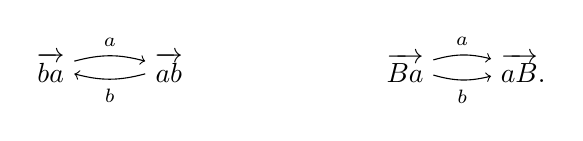
\begin{tikzpicture}[x=1.5cm]
      \node (ba) at (0,0) {$\ora{ba}$};
      \node (ab) at (1,0) {$\ora{ab}$};
      \node (Ba) at (3,0) {$\ora{Ba}$};
      \node (aB) at (4,0) {$\ora{aB}$.};
      \draw [->,bend left=15] (ba) to node[above,cdlabel]{a} (ab);
      \draw [->,bend left=15] (ab) to node[below,cdlabel]{b} (ba);
      \draw [->,bend left=15] (Ba) to node[above,cdlabel]{a} (aB);
      \draw [->,bend right=15] (Ba) to node[below,cdlabel]{b} (aB);
    \end{tikzpicture}
  \]
  The hyperbolic elements $a$ and~$b$ have north-south dynamics. Using
  this in the three cases depending on the relation of $\ora{a}$ and
  $\ora{b}$, we have the
  following.
  \begin{enumerate}[label=(\Roman*)]
  \item If $(\ora{a},\ora{b})$ R-cross, then we claim that the
    endpoints of the various geodesics must be laid out as in
    Figure~\ref{fig:cross}.

\begin{figure}
    \begin{subfigure}[b]{0.3\textwidth}
 \resizebox{\linewidth}{!}{\svgfignormal{rcrossing}}
    \caption{$\protect\ora{a}$ and $\protect\ora{b}$ R-cross}
    \label{fig:cross}
     \end{subfigure}
     \hfill
     \begin{subfigure}[b]{0.3\textwidth}
 \resizebox{\linewidth}{!}{\svgfignormal{parallel}}
    \caption{$\protect\ora{a}$ and $\protect\ora{b}$ are R-parallel }
    \label{fig:parallel}
\end{subfigure} 
\hfill
\begin{subfigure}[b]{0.3\textwidth}
 \resizebox{\linewidth}{!}{\svgfignormal{antiparallel}}
    \caption{$\protect\ora{a}$ and $\protect\ora{b}$ are R-anti-parallel }
    \label{fig:anti}
   \end{subfigure}
   \caption{Cases for relative position 
     of $\protect\ora{a}$ with $\protect\ora{b}$, and corresponding
     endpoints of products.}
   \label{fig:cases-a-b}
 \end{figure}
 
    To see this, by the dynamics of $a$ and $b$ on the
    circle as shown, $ba$ maps the interval
    $(b^+,a^+)$ strictly inside itself, so $ba$ is
    hyperbolic with $(ba)^+\in(b^+,a^+)$;
    similarly $(ba)^- \in (b^-,a^-)$. The actions of
    $b$ and $a$ interchange $(ba)^- \leftrightarrow (ab)^-$ and
    $(ba)^+ \leftrightarrow (ab)^+$, forcing the configuration shown.
    (Note that all four endpoints $(ba)^\pm,(ab)^\pm$ are on the
    portions of the circle
    where $b$ and $a$ move in opposite directions.)

    Since $(\ora{B},\ora{a})$ also R-cross, the
    other conclusion follows.
  \item If $(\ora{a},\ora{b})$ are R-parallel, then $ab \cdot (b^+,a^+) \subsetneq (b^+,a^+)$, so $ab$ is
    hyperbolic and $(ab)^+ \in (b^+,a^+)$. The same interchange
    property then forces
    $(ab)^+, (ba)^+ \in (b^+,a^+)$, as well as
    $(ab)^-, (ba)^- \in (a^-,b^-)$. From this we see that
    $(\ora{ba},\ora{ab})$ R-cross, as in Figure~\ref{fig:parallel}.
  \item If $\ora{a}$ and $\ora{b}$ are anti-parallel, we can reduce to
    the parallel case by replacing $b$ with $B$, arranged as in
    Figure~\ref{fig:anti}.\qedhere
  \end{enumerate}
\end{proof}

\subsection{Position of axes 
\texorpdfstring{$\protect\ora{aB}$}{aB} and \texorpdfstring{$\protect\ora{Ba}$}{Ba} in parallel  case}
\label{subsec:antiparallel}
If $\ora{a}$ and $\ora{b}$ are R-parallel,
Lemma~\ref{lem:righthandedfoundation} makes no claim about the
relationship of $\ora{aB}$ and $\ora{Ba}$. Indeed this is not
determined by the hypotheses: they can be crossing or anti-parallel
(Lemma~\ref{lem:aB_bA_antiparallel_cross}).
Nevertheless, we can extract some information about composite pairs.

Fix $a,b \in \Isom^+(\bbH^2)$ so that $\ora{a}$ and $\ora{b}$ are
R-parallel. We know that $ab$ and $ba$ are
hyperbolic (with crossing axes). Suppose also that $aB$ is hyperbolic. (This will be the case, for example, if $a,b \in \pi_1(S)$.)

\begin{figure}[hb]
  \centering
  \setlength{\abovecaptionskip}{3pt}
  \setlength{\belowcaptionskip}{0pt}

  \begin{subfigure}[t]{0.42\textwidth}
    \centering
    \resizebox{\linewidth}{!}{\svgfignormal{r3}}
    \caption{$\protect\ora{Ba},\protect\ora{aB}$ splitting}
    \label{fig:r3}
  \end{subfigure}
  \hfill
 \begin{subfigure}[t]{0.42\textwidth}
    \centering
    \resizebox{\linewidth}{!}{\svgfignormal{r1}}
    \caption{$\protect\ora{aB}$, $\protect\ora{Ba}$ are $b$-sided and antiparallel to each other}
    \label{fig:r1}
  \end{subfigure}
  \vspace{10pt}\par
  \begin{subfigure}[t]{0.42\textwidth}
    \centering
    \resizebox{\linewidth}{!}{\svgfignormal{c2}}
    \caption{$\protect\ora{aB}$, $\protect\ora{Ba}$ are $b$-sided and crossing}
    \label{fig:c2}
  \end{subfigure}

  \caption{Topological cases for the location of $\protect\ora{aB}$ and
    $\protect\ora{Ba}$ when $(\protect\ora{a},\protect\ora{b})$ are parallel.}
  \label{fig:cases-conn-smoothing}
\end{figure}

\begin{lemma}
If $(\ora{a},\ora{b})$ are parallel, $\ora{aB}$ does not cross $\ora{a}$ or $\ora{b}$.
\label{lem:aB_a_nocross}
\end{lemma}
\begin{proof}
If $\ora{aB}$ crossed $\ora{a}$, then $\ora{(bA)a}=\ora{b}$ would
cross $\ora{a}$, a contradiction. Similarly $\ora{aB}$ cannot cross $\ora{b}$.
\end{proof}

\begin{lemma}
If $(\ora{a},\ora{b})$ are parallel, for $g \in \{ a, b \}$, the
endpoints of $\ora{aB}$ and the endpoints of $\ora{Ba}$ are in the
same connected component of $\partial_\infty S - \{ g^+,g^-\}$.
\label{lem:aB_Ba_together}
\end{lemma}
\begin{proof}
  By the previous lemma, the endpoints of $\ora{Ba}$ are in one
  connected component.
  Since $a \cdot \ora{Ba} = b \cdot \ora{Ba} = \ora{aB}$, by NS dynamics of $a$ and $b$,
the endpoints of $\ora{aB}$ are in the same connected component.
\end{proof}

When $\ora{a},\ora{b}$ are R-parallel and
\[
\big((aB)^-,(aB)^+\big) \subsetneq (b^+,a^+)
\quad\text{and}\quad
\big((Ba)^-,(Ba)^+\big) \subsetneq (a^-,b^-),
\]
as in Figure~\ref{fig:r3}, we say that
\emph{$\ora{aB}$ splits $\ora{a},\ora{b}$}.
Similarly, whenever
\[
\big((aB)^-,(aB)^+\big),
\big((Ba)^-,(Ba)^+\big)
\subsetneq (b^-,b^+),
\]
as in Figure~\ref{fig:r1},
we say that \emph{$\ora{aB}$ is on the $b$-side of $\ora{a},\ora{b}$},
and we say that it \emph{is on the $a$-side of $\ora{a},\ora{b}$} if both intervals
are contained in $(a^+,a^-)$. When $\ora{a},\ora{b}$ are L-parallel
the terminology is adjusted accordingly. We will also use this
terminology for powers $\ora{a^n B^m}$ and $\ora{B^m a^n}$, which will
have the same division of cases since $\ora{a^n}$ and $\ora{a}$ have
the same axis.

\begin{lemma}
\label{lem:trichotomy_ab}
If $(\ora{a},\ora{b})$ are parallel, then $\ora{aB},\ora{Ba}$ are
exactly one of $a$-sided, splitting, or $b$-sided.
\end{lemma}
\begin{proof}
This follows from Lemma~\ref{lem:aB_Ba_together}.
\end{proof}

\begin{lemma}
\label{lem:aB_bA_antiparallel_cross}
If $(\ora{a},\ora{b})$ are parallel, then $(\ora{aB},\ora{Ba})$  are anti-parallel or cross.
\end{lemma}
\begin{proof}
By Lemma~\ref{lem:aB_Ba_together} and the fact that $a \cdot \ora{Ba} = \ora{aB}$,
it follows that $\ora{aB},\ora{Ba}$ cannot be nested with respect to $\ora{a}$.
Then since $a \cdot \ora{Ba} = \ora{aB}$, they must both be either parallel or anti-parallel to $\ora{a}$, so cannot be parallel to each other.
\end{proof}

See Figure~\ref{fig:c2} and Example~\ref{ex:ab_parallel_aB_crossing} for examples where $(\ora{Ba},\ora{aB})$ cross.

\begin{lemma}
If $(\ora{a},\ora{b})$ are parallel and $\ora{aB},\ora{Ba}$ are splitting,
then $(aB)^{\pm} \in (b^+, a^+)$ and $(Ba)^{\pm} \in (a^-,b^-)$.
\label{lem:splitting_specific}
\end{lemma}
\begin{proof}
This follows from $a \cdot \ora{Ba}= b \cdot \ora{Ba} =\ora{aB}$ and the fact that $a,b$ 
move in opposite directions (cw/ccw) on these intervals. The only way the $a$ and $b$ actions can end up in the same place is if they move from one interval to the other.
\end{proof}

To draw specific examples precisely, consider the common hyperbolic perpendicular of $\ora{a}$
and $\ora{b}$, which we will denote~$R_1$. We will also use the
same notation for the reflection through~$R_1$.
Let $R_2, R_3, R_4, R_5$ be the lines and corresponding reflections so
that $a=R_1 R_2 = R_4 R_1$, and $b=R_1 R_3 = R_5 R_1$. Precisely,
$R_2$ and $R_4$ are perpendicular to $\ora{a}$, and $R_3$ and $R_5$
are perpendicular to $\ora{b}$.

Since
$ab=R_4 R_3$, $ba=R_5 R_2$, $Ba=R_3 R_2$, and $aB=R_4 R_5$, and all of
these elements are hyperbolic, we see
that the $R_i$ are reflections along pairwise non-intersecting reflection
lines. There are several potential configurations, as shown
in Figure~\ref{fig:cases-conn-smoothing}.

We next show that by taking powers we can reduce to the splitting
case, starting with a general convergence lemma.

\begin{lemma}
\label{lem:convergence_action}
Let $g,x \in \PSL(2,\mathbb{R})$, with $x$ hyperbolic and
$g \cdot x^+ \neq x^-$. Then, for all sufficiently large $n$,
the element $x^n g$ is hyperbolic and
\[
\lim_{n \to \infty} (x^n g)^+ = x^+ .
\]
More generally, if $g,h,x \in \PSL(2,\bbR)$ with $x$ hyperbolic and
$hg \cdot x^+ \ne x^-$, then for all sufficiently large $n$, the
element $g x^n h$ is hyperbolic and
\begin{align*}
  \lim_{n \to \infty} (g x^n h)^+ &= g \cdot x^+, &
  \lim_{n \to \infty} (g x^n h)^- &= H \cdot x^-.
\end{align*}
If $x,g,h \in \pi_i(S)$, the hypotheses that $g \cdot x^+ \ne x^-$,
resp.\ $hg \cdot x^+ \ne x^-$, are automatic.
\end{lemma}

\begin{proof}
This follows from NS dynamics on $\partial_\infty S$.
Indeed, choose a neighborhood $V$ of $x^+$ such that
$x^- \notin g \cdot V$. Then, by NS, there is
$n_0>0$ such that, for every $n \ge n_0$,
\[
x^n g \cdot V \subsetneq V.
\]
Thus $x^n g$ is hyperbolic, with
\[
(x^n g)^+ \in x^n g \cdot V \subsetneq V.
\]
As $n \to \infty$, $x^n g \cdot V \to x^+$ and so $(x^n g)^+ \to x^+$.

For the more general statement, apply the first part of the statement
to $x^n hg$ and to $X^n GH$. Since
$g \cdot \ora{x^n hg} = \ora{g x^n h}$ and $H \cdot \ora{X^n GH} =
\ora{H X^n G}$, we get the claimed result.

If $g,x \in \pi_1(S)$, since each point in $\bdy_\infty S$ is the
endpoint of at most one geodesic, if $g \cdot x^+ = x^-$ then also $g
\cdot x^- = x^+$. But this implies that $g$ is elliptic of order~$2$,
which is impossible in a surface group. Similarly for the more general
statement.
\end{proof}


\begin{lemma}
Let $\ora{a},\ora{b}$ be parallel. If $\ora{a^nB^m}$ splits $\ora{a},\ora{b}$, then so does
$\ora{a^NB^M}$ for every $N \geq n$ and $M \geq m$.
\label{lem:once_splits}
\end{lemma}
\begin{proof}
It suffices to prove the claim for $\ora{a^{n+1}B^m}$ and $\ora{a^nB^{m+1}}$.
Note that $\ora{a},\ora{a^nB^m}$ being parallel implies
$(a^{n+1}B^m)^+ \in ((a^nB^m)^+, a^+) \subset (b^+, a^+)$.
Similarly, $\ora{a^nB^m},\ora{B}$ are parallel, so $(a^nB^{m+1})^- \in (B^-, (a^nB^m)^-) \subset (b^+,a^+)$
This proves the claim.
\end{proof}

\begin{proposition}
If $\ora{a}$ and $\ora{b}$ are parallel, then there exists $s > 0$ such that
$\ora{a^n B^m}$ is splitting for every $n,m \ge s$.
\label{prop:eventual_splitting}
\end{proposition}

\begin{proof}
By Lemma~\ref{lem:once_splits}, it suffices to show that there exist $n,m \geq 0$
such that $\ora{a^{n} B^{m}}$ is splitting.

Suppose for definiteness that $(\ora{a},\ora{b})$ are R-parallel.
Choose $m>0$ so that
\[
B^m \cdot a^- \in (b^+, a^+).
\]
Fix such an $m$. As $n \to \infty$, Lemma~\ref{lem:convergence_action} gives
\begin{align*}
\lim_{n \to \infty} (a^n B^m)^+ &= a^+, &
\lim_{n \to \infty} (a^n B^m)^- &= B^m \cdot a^-.
\end{align*}
In particular, for $n$ sufficiently large, we have
\[
(a^n B^m)^- \in (b^+, a^+),
\]
which implies that $\ora{a^n B^m}$ is splitting.
\end{proof}

\begin{remark}
A ping-pong argument~\cite[\S 8.2.E]{Gromov1987HyperbolicGroups}
shows that, in the splitting configuration, the subgroup generated by $a$ and $b$
is free.
Accordingly, Proposition~\ref{prop:eventual_splitting} is related to the existence
of an exponent $s>0$ (depending on $a,b$) such that, for all $m,n \ge s$,
the subgroup generated by $a^m$ and $b^n$ is free.

Results of this type hold in much greater generality, for instance for
Gromov hyperbolic groups and for mapping class groups; see, e.g.,
\cite{Fujiwara2015SubgroupsPseudoAnosovII}.
\end{remark}

From the above analysis, it follows that when $(\ora{a},\ora{b})$ are
parallel, many composite pairs are parallel. We can extract a
particular result we will use later.
\begin{lemma}\label{lem:a_parallel_Ba}
Let $a,b \in \pi_1(S)$.
If $\ora{a},\ora{b}$ are parallel and $(\ora{aB}, \ora{Ba})$ cross,
let $\mathcal{A} \coloneqq \{ \ora{a},\ora{b}, \ora{ab},\ora{ba} \}$
and $\mathcal{B} \coloneqq \{ \ora{aB}, \ora{Ba} \}$. Then either
\begin{itemize}
\item $(\ora{g},\ora{h})$ is parallel for every $\ora{g} \in \mathcal{A}, \ora{h} \in \mathcal{B}$; or
\item $(\ora{g},\ora{h})$ is anti-parallel for every $\ora{g} \in \mathcal{A}, \ora{h} \in \mathcal{B}$.
\end{itemize}
\end{lemma}
\begin{proof}
Since
$(\ora{aB},\ora{Ba})$ cross, they must be either $a$-sided or
$b$-sided.
If they are $a$-sided, then they are either parallel or anti-parallel to $\ora{a}$.
If they are parallel, since $\ora{ab}$, $\ora{ba}$, and $\ora{b}$ are parallel to
$\ora{a}$ and on the opposite side of $\ora{ab}$, we are in the first
case of the statement.
Otherwise we are in the second case.

If they are $b$-sided, the analysis is similar: just swap $a \leftrightarrow B$ and $b \leftrightarrow A$, since $(\ora{B},\ora{A})$ are parallel.
\end{proof}

Suppose that $\ora{Ba},\ora{aB}$ are $b$-sided and cross, as in Figure~\ref{fig:c2}. If we replace $b$ by $B$, we see that $\ora{ab}$ and
$\ora{ba}$ can cross even though $\ora{a}$ and $\ora{b}$ are not
parallel (in fact, they are anti-parallel). Let us show a concrete
example where this situation arises. See also the discussion
in~\cite{MGT25:SmoothingsErratum}.

\begin{example}
  To see that the case $b$-sided and crossing actually arises, consider any two parallel $\ora{g}$
  and $\ora{h}$, for instance coming from an appropriately-oriented
  pair of disjoint simple closed curves sitting
  as the cuffs of an embedded pair of pants.
  Define $a \coloneqq hghgh$ and $b
  \coloneqq hgh$. We claim that $\ora{a}$ and $\ora{b}$ are
  parallel. First, by
  Lemma~\ref{lem:righthandedfoundation}\ref{item:ab-parallel}, $\ora{hg}$ and $\ora{gh}$ cross and $\ora{h}$ and $\ora{gh}$ are
  parallel. Applying the lemma again to $(\ora{h},\ora{gh})$, we see
  that $\ora{hgh}$ and $\ora{gh}$ are parallel, and applying the lemma
  once more we see $\ora{b} = \ora{hgh}$ and $\ora{a} = \ora{hghgh}$
  are parallel, as desired. See Figure~\ref{fig:crossing_aB}.
  Finally, $aB=(hghgh)(HGH)=hg$ and $Ba=(HGH)(hghgh)=gh$, which cross,
  as desired.
  \label{ex:ab_parallel_aB_crossing}
\end{example}

\begin{figure}
\centering{
\svgfignormal{crossing_aB}
\caption{The proof that $\protect\ora{a} \coloneqq \protect\ora{hghgh}$ and
  $\protect\ora{b} \coloneqq \protect\ora{hgh}$ are parallel if
  $\protect\ora{g},\protect\ora{h}$ are parallel.}
\label{fig:crossing_aB}
}
\end{figure}


\subsection{Fundamental smoothing results}
\label{sec:fund-smoothing}

As part of our construction, we will use large powers of some fixed
elements. We collect some propositions guaranteeing essential
crossings in this context.

\begin{proposition}\label{prop:join-split-geom}
Let $a,b,x \in \pi_1(S)$ be curves with $\ora{a}$, $\ora{b}$
crossing $\ora{x}$ to the right. Then there is $s \ge 0$ (depending on $a,b,x$)
  so that, for all
 $n, m, r \in \mathbb{Z}$ with either $s < r < m-n-s$ or $m-n+s < r <
 -s$, we have
  \begin{align}
    \label{eq:cross-join} [a x^n] [b x^m] &\reducesto [ax^{n+r}bx^{m-r}]\\
    \label{eq:cross-split} [a x^nb x^m] &\reducesto [ax^{n+r}][bx^{m-r}].
  \end{align}

  There exists $s' \ge 0$ (depending on $a,x$) so that for all
  $|n-m| > s'$,
  \begin{align}
    \label{eq:cross-cancel}[ax^n][ax^m] &\reducesto [x^{|n-m|}].
  \end{align}

 If $x$ is simple and $a=b$, we may take $s=s'=0$. In particular, for
 all $n\in\bbZ$,
 \begin{align}
    [a x^{n+1}] [a x^{n-1}] &\reducesto 2[ax^{n}].\label{eq:cross-simple}
  \end{align}
\end{proposition}

Note that for the allowed values of $r$, Eqs.\ \eqref{eq:cross-join} and
\eqref{eq:cross-split} move the exponents $n,m$ closer to the diagonal
$m=n$.

We will make heavy use of the \emph{band model} centered on
$\ora{x}$, meaning the conformal map from $\bbH^2$ to a horizontal
strip $(-\infty,\infty) \times [-v,v]$ mapping $x^-$ to infinity along
the negative $x$-axis and $x^+$ to infinity on the positive $x$-axis.
We choose the \emph{normalized} band model, picking $v$ so that the
action of $x$ is horizontal translation by $z \mapsto z+1$.

For any geodesic $\ora{y}$ that is parallel to
$\ora{x}$, there is a \emph{window} $w(\ora{y})$ cut out by the
endpoints on the band model, the interval between $y^\pm$ that
misses~$x^\pm$. Observe that $w(x^k\cdot\ora{y})$ is the horizontal
translate of $w(\ora{y})$ by $k$. See Figure~\ref{fig:abcrossings} for
examples.

\begin{lemma}
  Given $a,b, x \in \pi_1(S)$ so that $\ora{a}$ and $\ora{b}$ cross $\ora{x}$ to
  the right and $g_1 = x^k ax^\ell$ with $k,\ell \in \bbZ$, we have
  $g_1^+ \in w(x^k a\cdot\ora{x})$ and
  $g_1^- \in w(x^{-\ell}A\cdot\ora{x})$. Similarly for
  $g_2 = x^k a x^\ell b x^n$ with $k,\ell,n\in\bbZ$, we have
  $g_2^+ \in w(x^ka \cdot \ora{x})$ and $g_2^- \in w(x^{-n} B
  \cdot\ora{x})$.
\label{lem:windows}
\end{lemma}

\begin{proof}
  For the first part, it suffices to show that $\ora{g_1}$ crosses
  $x^ka \cdot \ora{x}$ and $x^{-\ell} A\cdot \ora{x}$ to the right,
  or equivalently (by translation) that $\ora{x^{\ell+k}a}$ and $\ora{ax^{k+\ell}}$
  cross $\ora{x}$ to the right. This follows from
  Lemma~\ref{lem:rhs_prod}.

  For the second part, we similarly use Lemma~\ref{lem:rhs_prod} to
  see that $\ora{g_2}$ crosses $x^ka \cdot \ora{x}$ and $x^{-n}B \cdot
  \ora{x}$ to the right.
\end{proof}

\begin{figure}
\centering{
\resizebox{150mm}{!}{\svgfigbig{abliftsbands}}
\caption{The band model centered on $\protect\ora{x}$ used in
  Proposition~\ref{prop:join-split-geom}, in a case where $\protect [x]$ is simple.
  Some lifts of $\protect [x]$ are depicted in blue. The central blue lift
  is $\protect\ora{x}$, and we also show translates by $ \protect x^k a$, $\protect x^l
  A$, $\protect x^m b$ and $\protect x^n B$, together with their windows.
  If $\protect[x]$ is not simple, the blue lifts can intersect each other.}
\label{fig:abcrossings}
}
\end{figure}

\begin{proof}[Proof of Proposition~\ref{prop:join-split-geom}]
  In each case, we will show that we can choose lifts of the curves to
  the normalized band model for which a
  relevant crossing is essential. We start with
  Eq.~\eqref{eq:cross-join}, looking first at the windows $w(a\cdot
  \ora{x})$ and $w(x^rb\cdot\ora{x})$.
  Since each window is a
  finite size, there is a finite range $[s_1,s_2]$ so that $w(x^rb\cdot\ora{x})$
  is to the left of (resp.~to the right of) $w(a\cdot\ora{x})$ if $r < s_1$
  (resp.\ $r > s_2$).
  Similarly there
  is a range $[s_1',s_2']$ so that $w(A\cdot\ora{x})$ is disjoint from
  $w(x^rB\cdot\ora{x})$ if $r \notin [s_1',s_2']$, and the exponents determine the
  ordering of the windows. Set
  $s \coloneqq \max\{s_2,s_2',-s_1,-s_1'\}$.

  Now consider
  $g_1 = ax^n$ and $g_2 = x^rbx^{m-r}$, with $s < r < m-n-s$. We have
  \[
    r-m < -n-s \le -n+s_1',
  \]
  so, by Lemma~\ref{lem:windows}, $g_1^- \in w(x^{r-m}B\cdot\ora{x})$
  is to the left of $g_2^- \in w(x^{-n}A\cdot\ora{x})$, and
  \[
    s_2 \le s < r,
  \]
  so $g_1^+ \in w(x^rb\cdot\ora{x})$ is to the right of $g_2^+ \in
  w(a\cdot\ora{x})$. Thus
  $\ora{x^rbx^{m-r}}$ crosses $\ora{ax^n}$ to the left. Similarly if
  $m-n+s < r < -s$, then $\ora{x^rbx^{m-r}}$ crosses $\ora{ax^n}$ to the
  right. In either case,
  \[
    [ax^n][bx^m] = [ax^n][x^r bx^{m-r}] \reducesto [ax^{n+r}bx^{m-r}]
  \]
  by oriented disconnected smoothing.
  For Equation~\eqref{eq:cross-split}, write $[x^r ax^n bx^{m-r}]=[gh]$ with
  $g=x^r ax^n$ and $h=bx^{m-r}$, 
  so $g^+ \in w(x^ra\cdot\ora{x})$ and $g^- \in w(x^{-n}A \cdot \ora{x})$, and $h^+ \in w(b \cdot \ora{x})$, $h^- \in w(x^{r-m} B \cdot \ora{x})$.
  Hence, if $s < r < m-n-s$, we have $s_1 < r$
  so $w(b\cdot\ora{x})$ is to the left of $w(x^r a\cdot\ora{x})$,
  while $r-m < -n+s_1'$, so $w(x^{r-m}B \cdot\ora{x})$ is to the left
  of $w(x^{-n}A\cdot\ora{x})$, and hence $\ora{h}$ and $\ora{g}$ are R-parallel, giving Eq.~\eqref{eq:cross-split} by oriented connected smoothing.
  
  We similarly get parallelism if $m-n+s < r < -s$.

  To see Eq.~\eqref{eq:cross-cancel}, suppose without loss of generality
  that $n < m$. Let $s_0 = \lceil \wid(w(a\cdot\ora{x})) \rceil$
  (with width measured in the normalized band model),
  and
  let $s' = 2s_0 - 1$. Since $m-n \ge 2s_0$, we can pick $r$ so that
  $s_0 \le r \le m-n-s_0$. By the above argument, $\ora{ax^n}$ and
  $\ora{x^rax^{m-r}}$ R-cross (since, e.g., $(ax^n)^+ \in w(a\cdot\ora{x})$ and
  $(x^rax^{m-r})^+ \in w(x^r a\cdot\ora{x})$, which are disjoint), so we get the
  desired smoothing in Eq.~\eqref{eq:cross-cancel} by using unoriented
  disconnected smoothing.

  In the cases when $x$ is simple, two windows are disjoint, nested,
  or identical; this implies that $s_1 = s_2$ and $s_1' = s_2'$.
  If in
  addition $a=b$, we also see that $s_1=s_1'=0=s$. This gives Eqs.\
  \eqref{eq:cross-join} and \eqref{eq:cross-split}, and the special
  case Eq.\ \eqref{eq:cross-simple}.

  To see that with $x$ simple we get Eq.\ \eqref{eq:cross-cancel} with
  $s'=0$ (i.e., $[ax^n][ax^{n+1}] \reducesto [x]$), we look slightly deeper
  in the words. The analysis above shows $(ax^n)^- \in
  w(x^{-n}A\cdot\ora{x})$, which is to the right of
  $(ax^{n+1})^- \in w(x^{-n-1}A\cdot\ora{x})$. By
  looking at the band model centered on $a \cdot \ora{x}$ (or
  equivalently by conjugating by $a$), we see that
  $(ax^n)^+ \in w(ax^na\cdot\ora{x}) \subset w(a\cdot\ora{x})$. Similarly
  $(ax^{n+1})^+ \in w(ax^{n+1}a\cdot\ora{x}) \subset
  w(a\cdot\ora{x})$. We therefore have that $(ax^n)^+$ is to the left
  of $(ax^{n+1})^+$, implying that $\ora{ax^n}$ crosses $\ora{ax^{n+1}}$ as
  desired.
\end{proof}

We also need some results about smoothings where we have high powers of
two different elements. We work with three elements $a,x,y\in\pi_1(S)$
so that $(\ora{y},\ora{x},a\cdot\ora{y})$ are R-parallel; this
implies, for instance, that $(a\cdot\ora{y},a\cdot\ora{x})$ are also
R-parallel.
We again consider the normalized band model
centered on~$\ora{x}$, starting with another lemma about endpoints.

\begin{lemma}\label{lem:ayx-window}
  For any triple $a,x,y\in\pi_1(S)$ so that
  $(\ora{y},\ora{x},a\cdot\ora{y})$ are R-parallel, and for
  $\ora{g}=\ora{x^k ay^n x^\ell}$ with $k,\ell,n\in\bbZ$, we have
  $g^+ \in w(x^k a \cdot\ora{y})$ and
  $g^- \in w(x^{-\ell}\cdot\ora{y})$.
\end{lemma}

\begin{proof}
  Let $v = x^{-\ell} \cdot (y^-,y^+)$, the \emph{complement}
  of $w(x^{-\ell} \cdot \ora{y})$.
  We have
  $g \cdot v = x^k ay^n \cdot(y^-,y^+) = x^k a\cdot (y^-,y^+) = w(x^k a \cdot
  \ora{y}) \subset (x^-,x^+) \subsetneq v$,
  proving the result by Lemma~\ref{lem:NS-dynamics}.
\end{proof}

\begin{proposition}\label{prop:fundamental-ayx}
  For any triple $a,x,y\in\pi_1(S)$ so that $(\ora{y},\ora{x},a\cdot\ora{y})$ are R-parallel, there exists
  $s \ge 0$ so that for all $r > s$ and $m,n \in \bbZ$,
  \begin{align}
    \label{eq:crossuniform_n}
       [a y^m x^{n+r}][a y^m x^{n-r}] &\reducesto [(a y^m x^n)^2]\\
    \label{eq:crossuniform_m}
       [a y^{m+r} x^n][a y^{m-r} x^n] &\reducesto [(a y^m x^n)^2].
  \end{align}
  Furthermore, for $n,m \ge s$,
  \begin{align}\label{eq:cancel-ayx}
    [a y^m x^n][A] &\reducesto [y^m][x^n]\\
    \intertext{and for $n,m > 2s$,}
    \label{eq:crossbelowy}
    [a Y^m x^n][A] &\reducesto [x^s Y^s] [A x^s a Y^s] [x^{n-2s}] [Y^{n-2s}]
  \end{align}
\end{proposition}

\begin{proof}
  We first prove Eq.~\eqref{eq:crossuniform_n}. We will have a number
  of windows $w(x^m \cdot \ora{y})$ on the top, all of equal width
  in the normalized band model, and $w(x^m a \cdot \ora{y})$ on the
  bottom, also of equal widths (but not necessarily equal to widths on
  the top). Take
  \[
    s \ge \max(\wid(w(\ora{y})),
    \wid(w(a\cdot\ora{y}))).
  \]
  For $r > s$, consider the elements $g_1 = x^n ay^m x^r$ and $g_2 =
  x^{n-r} a y^m$. By Lemma~\ref{lem:ayx-window}, we have
  \begin{align*}
    g_1^+ &\in w(x^n a\cdot\ora{y}) & g_1^- &\in w(x^{-r}\cdot\ora{y})\\
    g_2^+ &\in w(x^{n-r} a \cdot\ora{y}) & g_2^- &\in w(\ora{y}).
  \end{align*}
  Since $r>s$, the endpoints appear in the cyclic order
  $(x^-,g_2^+,g_1^+,x^+,g_2^-,g_1^-)$ on $\partial_\infty S$. In
  particular $[g_1][g_2] \reducesto [g_1 g_2]$ by oriented disconnected smoothing, as desired.
  
  To see Eq.~\eqref{eq:crossuniform_m}, apply
  Eq.~\eqref{eq:crossuniform_n} with the change of variables
  $a' = a$, $y' = x$, and $x' = ayA$.
  This gives the desired result, after possibly increasing~$s$.

  For Eq.~\eqref{eq:cancel-ayx}, we consider $g = a y ^m x^n$ and
  compare its endpoints to those of $a$. By
  Lemma~\ref{lem:ayx-window}, we have
  $g^- \in w(x^{-n} \cdot \ora{y})$, which for large enough $n$ is to
  the left of $a^- \in w(\ora{y})$. For $g^+$,
  we again have to look deeper at the endpoints: since
  $g \cdot (x^+,x^-) = a y^m \dot (x^+, x^-) = w(a y^m \cdot
  \ora{x})$, we have
  $g^+ \in w(a y^m \cdot \ora{x}) \subset w(a \cdot \ora{y})$.
  Similarly $a^+ \in w(a \cdot \ora{x}) \subset w(a \cdot \ora{y})$.
  Considering the bands model centered on $a \cdot \ora{y}$ shows that,
  for $m$ large enough, $g^+$ is to the right of $a^+$, and thus
  $\ora{g}$ crosses $\ora{a}$ to the right. Thus if $s$ is large
  enough and $n,m
  \ge s$ we therefore have
  \[
    [a x^n y^m][A] = [g][A] \reducesto [x^n y^m] \reducesto [x^n][y^m]
  \]
  by oriented disconnected smoothing and then (by
  Lemma~\ref{lem:righthandedfoundation}) oriented connected
  smoothing.

  Finally, we see Eq.~\eqref{eq:crossbelowy}. By
  Proposition~\ref{prop:eventual_splitting}, if $s_0$ is large enough, for every $s \geq s_0$
  $\ora{Y^s x^s}$ and $\ora{x^s Y^s}$ split $\ora{y},\ora{x}$, and
  similarly $\ora{A x^s a Y^s}$ and $\ora{Y^s A x^s a}$ split $A \cdot
  \ora{x}, \ora{y}$; see
  Figure~\ref{fig:crossing_yx_A}. Furthermore, by a similar but easier window
  analysis as for Eq.~\eqref{eq:cancel-ayx}, if $s$ is large enough
  and $n > 2s$, $\ora{a}$ crosses $\ora{x^s a Y^m x^{n-s}}$.
  For $n,m > 2s$, we
  then have
  \begin{align*}
    [a Y^m x^n] [a] &= [x^s a Y^m x^{n-s}] [a] \\
    &\reducesto [A x^s a Y^m x^{n-s}]
      &&\text{$(\ora{a}, \ora{x^s a Y^m x^{n-s}})$ cross}\\
    &\reducesto [A x^s a Y^s] [Y^{m-s} x^{n-s}]
      &&\text{$(\ora{A x^s a Y^s}, \ora{Y^{m-s} x^{n-s}})$ parallel}\\
    &\reducesto [A x^s a Y^s] [Y^{m-s} x^s] [x^{n-2s}]
      &&\text{$(\ora{Y^{m-s} x^s}, \ora{x^{n-2s}})$ parallel}\\
    &\reducesto [A x^s a Y^s] [Y^{m-2s}] [Y^s x^s] [x^{n-2s}]
      &&\text{$(\ora{Y^{m-2s}}, \ora{Y^s x^s})$ parallel.} \qedhere
  \end{align*}
\end{proof}

\begin{figure}
\centering{
\resizebox{100mm}{!}{\svgfigbig{crossing_yx_A}}
\caption{Configuration  $\protect\ora{Y^s x^s}$ and $\protect\ora{x^s Y^s}$ splitting $\protect\ora{y},\protect\ora{x}$, and
   $\protect\ora{A x^s a Y^s}$ and $\protect\ora{Y^s A x^s a}$ splitting $A \cdot
  \protect\ora{x}, \protect\ora{y}$, used in Proposition~\ref{prop:fundamental-ayx}}
\label{fig:crossing_yx_A}
}
\end{figure}

In practice we will apply Proposition~\ref{prop:fundamental-ayx} with
four group elements.
\begin{corollary}\label{cor:fund-axby}
  Let $a,b,x,y \in \pi_1(S)$ be chosen so that $(B\cdot \ora{x},
  \ora{y}, a\cdot\ora{x})$ are R-parallel.
  Then there exists
  $s \ge 0$ so that for all $r > s$ and $m,n \in \bbZ$,
  \begin{align}
    \label{eq:axby-cross-n}
       [a x^{n+r} by^m][ax^{n-r} by^m] &\reducesto [(ax^n by^m)^2]\\
    \label{eq:axby-cross-m}
       [ax^n by^{m+r}][ax^n by^{m-r}] &\reducesto [(ax^n by^m)^2].
  \end{align}
  Furthermore, for $n,m \ge s$,
\begin{align}\label{eq:cancel-axby}
  [a x^n b y^m][ab] &\reducesto [x^n][y^m]\\
  \intertext{and for $n,m > 2s$,}
  \label{eq:crossbelowy-ab}
   [a x^n b Y^m][ab] &\reducesto [a x^s A Y^s] [B x^s b Y^s] [x^{n-2s}] [Y^{n-2s}]
\end{align}
\end{corollary}

\begin{proof}
  The conditions imply that
  $(\ora{y}, a \cdot \ora{x}, ab \cdot \ora{y})$ are R-parallel.
  Apply $x' = axA$, and $a' = ab$ to Eqs.~\eqref{eq:crossuniform_n},  \eqref{eq:crossuniform_m}, \eqref{eq:cancel-ayx} and~\eqref{eq:crossbelowy-ab} in order to get, respectively, Eqs.~\eqref{eq:axby-cross-n}
    \eqref{eq:axby-cross-m}
    \eqref{eq:cancel-axby} and~\eqref{eq:crossbelowy}.
\end{proof}

We now check this configuration is easy to find. The following result
is standard.

\begin{lemma}
The action of $\pi_1(S)$ on $\partial_{\infty} S$ is minimal,
i.e., for any $p \in \partial_{\infty} S$, the orbit
$\pi_1(S)\cdot p$ is dense.
\label{lem:minimal}
\end{lemma}

We care about the orientations, so we need a slightly more precise result.

\begin{lemma}
Let $x \in \pi_1(S)$.
Given any $z \in \partial_\infty  S$
and any $\epsilon>0$, there exists a lift $g \cdot \ora{x}$ whose
endpoints $g\cdot x^+$ and $g\cdot x^-$ are in $(z-\epsilon,z+\epsilon)$, and are ordered counter-clockwise (or clockwise)
with respect to the $\partial_\infty S$ order.
\label{lem:diagonaldense}
\end{lemma}
\begin{proof}
By Lemma~\ref{lem:minimal}, endpoints of axes of elements of
$\pi_1(S)$ are dense in $\partial_\infty S$; choose any $g$ so that
$g^+ \in (z-\epsilon,z+\epsilon)$. Next choose any $h$ so that
$\ora{h}$ crosses $\ora{g}$. Then for sufficiently large $k$, $h^{\pm k}\cdot
\ora{x}$ will be in a neighborhood of $h^{\pm}$ and in particular will
not cross $\ora{g}$.
Finally, for large enough $n$, we have
that $g^n h^{\pm k} \cdot x^{\pm} \in (z-\epsilon,z+\epsilon)$.
Tracing through orientations shows that one of these translates will
be clockwise and the other will be counterclockwise.
\end{proof}

\begin{lemma}\label{lem:initial}
  Given $x, y \in \pi_1(S)$, there exist $a,b \in \pi_1(S)$ so that
  $(B \cdot \ora{x}, \ora{y}, a \cdot \ora{x})$ are R-parallel.
\end{lemma}
\begin{proof}
  Immediate from Lemma~\ref{lem:diagonaldense}.
\end{proof}

%%% Local Variables:
%%% mode: latex
%%% TeX-master: "Intersections"
%%% End:

\section{Boxes and their measures}
\label{sec:define_measure}
Our main goal in the paper is to define a measure on the space of geodesics---in fact, a geodesic current---associated to a curve functional~$f$. 
Roughly speaking, our strategy is to associate a positive number, in a
countably additive way, to a collection of boxes of geodesics that is 
sufficiently rich to generate the $\sigma$-algebra of open sets of
$G(\Sigma)$.

To define the measure of our elementary boxes, we look at the
functional~$f$ applied to longer and longer curves~$C_i$. The
measure of a box is a linear combination of $f(C_i)$ chosen so that
the highest growth term vanishes, and the limit of interest picks out
the next asymptotics. This is reminiscent to the construction of Otal
\cite{Otal90:SpectreMarqueNegative}.

\subsection{Right-handed boxes}
\label{sec:boxes}

We now outline of the construction of the ``sufficiently rich family of boxes'' on which our measure will be defined.

Let $f\colon \Curves^+(S) \to \mathbb{R}$ be a
functional satisfying symmetry, additive union, smoothing and stability.
Fix
(arbitrarily) a simple closed oriented curve~$[x]$ which for convenience we take passing through the basepoint. The endpoints of the lifts of $[x]$ are dense in
$\partial_\infty S$, by minimality of the action of $\pi_1(S)$
(reviewed in Lemma~\ref{lem:minimal}).

The prototype for
the kind of boxes to which we assign measures is shown in
Figure~\ref{fig:newmodel3}: we have four geodesics, all lifts of~$[x]$, with
two lifts $\ora{\ell_1},\ora{\ell_2}$ on the left and two $\ora{r_1},\ora{r_2}$ on the right,
and consider the window
$[\ell_1^-,\ell_2^-) \times [r_2^+,r_1^+) \subset
\partial_\infty S \times \partial_\infty  S$ as a basic domain
for defining the measure.
(Recall that we give the endpoints of intervals in counterclockwise
order.)

The lifts are defined by a 4-tuple of
elements $[p_1,q_1,p_2,q_2]$ of $\pi_1(S)$ by
$\ell_i = P_i \cdot \ora{x}$ and $r_i = q_i \cdot \ora{x}$, with
conditions explained below.

\begin{figure}
\centering{
\resizebox{100mm}{!}{\svgfig{newmodel3}}
\caption{Schematically determining a RH box from group theory data
  with different lifts of a single curve $\protect[x]$. There are no
  constraints on how the base lift $\protect\ora{x}$ sits with respect to the
  other lifts. The other four lifts have constraints in how they
  sit; some other possibilities are shown in Figure~\ref{fig:rhbox}.
  Recall from Section~\ref{sec:actions} that the thicker arrows denote
the \emph{right} action of $\pi_1$.}
\label{fig:newmodel3}
}
\end{figure}

The measure that we ultimately assign to the associated windows will
be invariant under
\begin{subequations}\label{eq:changes}
\begin{align}
\text{(changing $p_i$ preserving $\ell_i$)} \quad & p_i \mapsto xp_i, \label{eq:changes-p}\\
\text{(changing $q_i$ preserving $r_i$)} \quad & q_i \mapsto q_ix. \label{eq:changes-q}
\end{align}
\end{subequations}
These two conditions are clearly necessary since the endpoints of $\ell_i$ and $r_i$ are invariant under such transformations.
In fact, ultimately we will take a limit of these
transformations: we look at the limit as $n\to \infty$ of $p_i \mapsto x^np_i$
and $q_i \mapsto q_i x^n$.

The measure $\mu$ will also be $\pi_1(S)$ invariant, which translates to
invariance under
(left-)translating all the lifts by $g \in \pi_1(S)$:
  \begin{equation}\label{eq:box-translate}
    (p_1,q_1,p_2,q_2) \mapsto g \cdot (p_1,q_1,p_2,q_2) \coloneqq
      (p_1 G, gq_1, p_2 G,  gq_2).
  \end{equation}
We will put off imposing this last invariance for the moment.

We now turn to the conditions on the lifts; for
instance, the window
$[\ell_1^-,\ell_2^-) \times [r_2^+,r_1^+)$ must avoid the
diagonal.

\begin{definition}\label{def:RH-lift-system}
  A \emph{right-handed lift system} (RH lift system) is a collection of elements
  $(p_1,q_1,p_2,q_2)$ in $\pi_1(S)$ so that
  \begin{enumerate}
  \item\label{item:box-nontriv-lift} $p_1P_2$ and $Q_1q_2$ are not powers of~$x$;
  \item\label{item:box-edges-cross-lift} for $i,j \in \{1,2\}$,
    $(\ora{p_iq_j},\ora{x})$ R-cross; and
  \item\label{item:box-diags-cross-lift} for sufficiently large~$n$,
    $(\ora{q_2x^np_1},\ora{q_1x^np_2})$ R-cross.
  \end{enumerate}
\end{definition}

See Figure~\ref{fig:rhbox} for examples of
RH systems, and Figure~\ref{fig:box4} for a non-example.
 We
distinguish three types of RH systems: \emph{type 1} has
no nested lifts of $[x]$; \emph{type 2} has one parallel pair of nested lifts; and
\emph{type 3} has two parallel pairs of nested lifts.
Note that since $[x]$ is simple, lifts
cannot intersect each other, and nested lifts cannot be anti-parallel
by condition \ref{item:box-edges-cross-lift}.


\begin{figure}
     \centering
\resizebox{40mm}{!}{\svgfig{box1}}
\quad
     \resizebox{40mm}{!}{\svgfig{box}}
\quad
\resizebox{40mm}{!}{\svgfig{box4}}
     \caption{Examples of right-handed boxes, of Type 1 (left), Type 2
     (middle), and Type 3 (right).}
     \label{fig:rhbox}
\end{figure}

\begin{figure}
  \centering{
\resizebox{45mm}{!}{\svgfig{box3}}
\caption{Non-example of right-handed box. It is a non-example because $\protect\ora{p_2q_1}$ does not cross $\protect\ora{x}$
  essentially (to the right or to the left)}
\label{fig:box4}
}
\end{figure}

\begin{definition}\label{def:RH-box}
  Every right handed lift system
  $(p_1,q_1,p_2,q_2)$ determines a
  \emph{right-handed box} of oriented geodesics in
  $\partial_{\infty} \Sigma \times \partial_{\infty} \Sigma - \Delta$, 
  given by \[
  B(p_1,q_1,p_2,q_2)=[\ell_1^-,\ell_2^-) \times [r_2^+,r_1^+),\] where $\ora{\ell_i} = P_i \cdot \ora{x}$ and $\ora{r_i} = q_i \cdot \ora{x}$.
 (On occasion, we may write $B_x(p_1,q_1,p_2,q_2)$ to make the choice of base element explicit.)
The set of all right-handed boxes is denoted by $\mathcal{B}$.
\end{definition}

\begin{remark}
\label{rmk:box_from_system}
Modifying the right-handed lift system by changing $p_i$ by
Eq.~\eqref{eq:changes-p} or changing $q_i$ by Eq.~\eqref{eq:changes-q} determines
the same right-handed box. Conversely, choices of the $p_i$/$q_i$
determining the same RH box are related in this way.
\end{remark}

The conditions in Definition~\ref{def:RH-lift-system} are chosen to
make the following proposition work.

\begin{proposition}\label{prop:rh-boxes}
  A tuple $(p_1,q_1,p_2,q_2)$ determines an RH lift system if and only if $\ora{\ell_i} =
  P_i \cdot \ora{x}$ and $\ora{r_i} = q_j \cdot \ora{x}$. Then the
  endpoints $\ell_1^-, \ell_2^-, r_2^+, r_1^+$ appear in that
  counter-clockwise order. In particular RH boxes in $\cB$ avoid the
  diagonal.
\end{proposition}

\begin{proof}
  We first note that condition~\ref{item:box-nontriv-lift} guarantees that $\ora{\ell_1} \ne \ora{\ell_2}$ and $\ora{r_1} \ne \ora{r_2}$. Also, condition~\ref{item:box-edges-cross-lift} implies
  that for any $i,j \in \{1,2\}$, $\ora{x}$ and $p_iq_j\cdot \ora{x}$
  are R-parallel (Lemma~\ref{lem:rhs}) and thus (by translation by
  $P_i$) that $(\ora{\ell_i}, \ora{r_j})$ are R-parallel.

  To exploit condition~\ref{item:box-diags-cross-lift}, we prove a lemma.
  
  \begin{lemma}\label{lem:box-endpoints}
    Suppose $p,q \in \pi_1(S)$ so that $(\ora{pq},\ora{x})$ R-cross.
    Set $\ell = Pxp$, $r = qxQ$, and
    for $n \in \bbZ$ set $g_n \coloneqq q x^n p$. Then
    \begin{align*}
      \lim_{n^+} g_n^- &= \ell^- &
      \lim_{n^+} g_n^+ &= r^+.
    \end{align*}
  \end{lemma}

  \begin{proof}
  For the second statement, apply Lemma~\ref{lem:convergence_action} with $x=qxQ$ and $g=qp$.
  For the first statement, apply it with $x=PXp$ and $g=PQ$.
  \end{proof}

  Returning to the proof of Proposition~\ref{prop:rh-boxes}, set
  $g_{i,j,n} \coloneqq q_j x^n p_i$.
  Condition~\ref{item:box-diags-cross-lift} says that for sufficiently large $n$
  the endpoints $g_{1,2,n}^-, g_{2,1,n}^-, g_{1,2,n}^+, g_{2,1,n}^+$
  appear in that ccw order, which by Lemma~\ref{lem:box-endpoints} implies
  that $\ell_1^-,\ell_2^-,r_2^+,r_1^+$ appear in that order, as desired.
\end{proof}

\begin{remark}
 Condition~\ref{item:box-diags-cross-lift} is
 phrased as it is to ensure translation invariance for boxes of type~2
 and type~3: $\ora{q_2 x^n p_1}$ and $\ora{q_1 x^n p_2}$ might only cross for large
 enough~$n$.
 For boxes of type~1, the crossing is essential for all~$n$.
\label{rmk:largeenough}
\end{remark}

\begin{remark}
  The reader may wonder why we choose to make the boxes half-open in
  the specified way. It turns out we could have made a different choice and it would not matter for the resulting current, as by
  Proposition~\ref{prop:spikes}
  the weight of the
  boundary of these boxes under any geodesic current is necessarily
  zero: the only lift of closed geodesics with an endpoint starting at one of the endpoints of the box is a single lift of~$[x]$, and by definition, these lifts are not contained in an RH box. The half-open
  choice we made is
  more convenient the proof of Proposition~\ref{prop:countablyadditive}.
  \label{rmk:no_atom_boundary_box}
\end{remark}

\begin{proposition}
The family of right handed boxes~$\mathcal{B}$ is dense in the space
of rectangles in $G(S)$, in the following sense. For any
$v_1,v_2,w_2,w_1\in \bdy_\infty S$ in that cyclic order,
and any $\epsilon>0$ so the respective $\epsilon$-neighborhoods are
disjoint, there exist $p_1,p_2,q_1,q_2 \in \pi_1(S)$ forming a
type~1 RH box $B(p_1,q_1,p_2,q_2)$ so that $p_i\cdot x^- \in B_\epsilon(v_i)$
and $q_j\cdot x^+ \in B_\epsilon(w_j)$.
\label{prop:density}
\end{proposition}
\begin{proof}
  By Lemma~\ref{lem:diagonaldense}, we can find translates
  $\ora{\ell_i} = P_i\cdot \ora{x}$ and $\ora{r_j} = q_j \cdot \ora{x}$ with both endpoints in
  the respective $\epsilon$-neighborhoods of the $v_i$ and $w_j$.
  Furthermore, that same lemma lets us arrange the orientations so
  that $\ora{\ell_i}$ and $\ora{r_j}$ are R-parallel, thus forming a
  RH lift system of type~$1$.
\end{proof}

\begin{figure}
\centering{
\resizebox{60mm}{!}{\svgfig{approxfin}}
\caption{Approximating a boundary point of the interval of endpoints of a right-handed box}
\label{fig:approx2}
}
\end{figure}

We now turn to invariance under translation by $\pi_1(S)$, as in
Eq.~\eqref{eq:box-translate}. The $\pi_1(S)$-orbit of $(p_1,q_1,p_2,q_2)$
can be parameterized by group elements $(a,b,c,d)$ related
  to the $p_i$ and $q_i$ by
\begin{equation}
\begin{aligned}
  a &= p_1 q_1 &\qquad\qquad\qquad\qquad\qquad b &= p_1 q_2\\[2pt]
  c &= p_2 q_1 & d &= p_2 q_2.
\end{aligned}
  \label{eq:relationdatum}
\end{equation}

\begin{figure}
\centering{
\resizebox{100mm}{!}{\svgfig{newmodel3_orbits}}
\caption{Parameterizing an RH orbit via elements $a,b,c,d$. The original position of $\protect\ora{x}$ is arbitrary, but the particular lifts determining the box fall into a type 1. Compare with Figure~\ref{fig:newmodel3}.}
\label{fig:newmodel3_orbit}
}
\end{figure}

Compare Figure~\ref{fig:newmodel3_orbit}. In this parameterization, we necessarily have $aCbD = 1$.
Note that, by Eq.~\eqref{eq:double_coset}, the relative position
of (say) $\ora{\ell_1}$ and $\ora{r_1}$ is given by the double coset
$\langle x \rangle a \langle x \rangle$.

Note that, for instance, the points $\wt \ast \cdot p_1^{-1}$ and $\wt \ast \cdot q_1$ are related via $a$ by the right action: $(\wt \ast \cdot p_1^{-1}) \cdot a = \wt \ast \cdot q_1$.
On the other hand, the lifts of $[x]$ give by $\ora{\ell_1}$ and
$\ora{r_1}$ are related via the element $q_1 p_1$ by the left action:
$q_1 p_1 \cdot \ora{\ell_1} = \ora{r_1}$. Furthermore, $(\ora{\ell_1},\ora{r_1})$ are R-parallel, which is equivalent (by Lemma~\ref{lem:rhs}) to $p_1 \cdot \ora{q_1 p_1} = \ora{p_1 q_1} = \ora{a}$ R-crosses $\ora{x}$.

The action of translating all lifts by $\pi_1(S)$ has been baked in to
this alternate parametrization,
but the measure corresponding to the associated window should be
invariant under the following four transformations:
\begin{subequations}\label{eq:translations}
\begin{align}
\text{(translating along $\ell_1$)} \quad & a \mapsto xa,\quad b \mapsto xb \label{eq:translations-l1}\\
\text{(translating along $\ell_2$)} \quad & c \mapsto xc,\quad d \mapsto xd \label{eq:translations-l2}\\
\text{(translating along $r_1$)} \quad & a \mapsto ax,\quad c \mapsto cx \label{eq:translations-r1}\\
\text{(translating along $r_2$)} \quad & b \mapsto bx,\quad d \mapsto dx \label{eq:translations-r2}
\end{align}
\end{subequations}
Conversely, given elements $a,b,c,d \in \pi_1(S)$ with
$aCdB = 1$, we can
construct four lifts of $[x]$ related by Equation~\eqref{eq:relationdatum}, for instance
setting $p_1 = 1$, $q_1 = a$, $q_2 = b$, and $p_2 = cA$.


\begin{definition}[RH orbit]
\label{def:RH-lift-sys}
Let $a,b,c,d \in \pi_1(S,\ast)$ be such that:
\begin{enumerate}[label=(\arabic*${}'$),start=0]
\item\label{item:box-close} $a C d B = 1$;
\item\label{item:box-nontriv} $aC(=bD)$ and $Ab(=Cd)$ are not powers of~$x$;
\item\label{item:box-edges-cross} $\ora{a},\ora{b},\ora{c},\ora{d}$ cross $\ora{x}$ to the right; and
\item\label{item:box-diags-cross} for sufficiently large~$n$,
  $\ora{dx^na C}
  (= \ora{cAbx^na C})$ crosses
  $\ora{cx^n}$ to the right.
\end{enumerate}

Then we call the datum $[a,b,c,d]$ a \emph{right-handed lift orbit} (or \emph{RH orbit}, for short).
\end{definition}

As explained above, this determines a $\pi_1(S)$-orbit of RH lift systems.
The one non-obvious point to check is that
condition~\ref{item:box-diags-cross} corresponds
to condition~\ref{item:box-diags-cross-lift}:
\begin{align*}
  cx^n &= p_2 q_1 x^n& dx^naC &= p_2 q_2 x^n p_1 P_2\\
  \intertext{which after conjugating by $P_2$ yields}
  q_1 x^n p_2 &= g_{2,1,n} & q_2 x^n p_1 &= g_{1,2,n}.
\end{align*}
Thus the two crossing conditions are equivalent.

\begin{definition}
  Let $B = B(p_1,q_1,p_2,q_2)$ be an RH box. The \emph{$\pi_1(S)$-orbit of $B$}
  \[
    [B] \;=\; \{ g \cdot B \colon g \in \pi_1(S) \},
  \]
  where we consider the left action.
  We write $[B(p_1,q_1,p_2,q_2)]$ to emphasize a chosen representative, or $[B]_{a,b,c,d}$ to emphasize the RH orbit. (On occasion we might write $[B_x]_{a,b,c,d}$ to be explicit about the base element $x$).
\end{definition}

\begin{remark}\label{rmk:flip_rh_box}
Even though in the sequel we will fix our base element to be $x$ once and for all, we observe that flipping an RH orbit with respect to $x$ gives a new RH orbit with respect to $x^{-1}$, in the following sense.
Let $[a,b,c,d]$ define an RH orbit with respect to the fixed element $x \in \pi_1(S)$.
Then the datum $[a', b', c', d']$ with $a' \coloneqq D$, $b' \coloneqq B$, $c'\coloneqq C, d'\coloneqq A$ is an RH orbit with respect to the base element $x' \coloneqq X$. Similarly, if $[p_1,q_1,p_2,q_2]$ is an RH lift system in the RH orbit $[a,b,c,d]$ with base element $x$, the datum $[p_1',q_1',p_2',q_2']$
where $p_1' \coloneqq Q_2$, $p_2' \coloneqq Q_1, q_1' \coloneqq P_2, q_2' \coloneqq P_1$
is an RH system with RH orbit $[a',b',c',d']$ and basepoint $x'$.
From this, one immediately has
\[B_x(p_1,q_1,p_2,q_2)=\sigma\bigl(B_{x'}(p_1',q_1',p_2',q_2')\bigr),\]
where $\sigma$ is the flip map.
\end{remark}

\subsection{Measures of boxes}

We will now start setting up the definition of the measure of an orbit
of right-handed box $[B]_{a,b,c,d}$. In particular, we will define a function
$\wh{\mu_f} \colon \mathcal{B} \to \mathbb{R}_{\geq 0}$ in terms of a limit
involving the $f$-value of a certain combination of words involving
$a,b,c,d,x$. (Recall $\mathcal{B}$
denotes the family of right-handed boxes.)

\begin{proposition}
\label{prop:limitexists}
Let $B(p_1,q_1,p_2,q_2)$ be a right-handed box so that $[B(p_1,q_1,p_2,q_2)]=[B]_{a,b,c,d}$.
Then following limit exists and only depends on the $\pi_1(S)$-orbit
of the box:
\begin{equation}
\wh{\mu_{f}}(B(p_1,q_1,p_2,q_2))\coloneqq\frac{1}{2}\lim_{n \to \infty}f([bx^n]) + f([cx^n])-f([ax^n]) - f([dx^n]).
\label{eq:def_measure}
\end{equation}
\end{proposition}
Note this function on boxes (which will eventually become a pre-measure and
then a measure) is automatically (left) $\pi_1(S)$-invariant.

We will now prove the limit in Proposition~\ref{prop:limitexists} exists using the properties
of~$f$ introduced in Section~\ref{subsec:mainhypotheses} and the
results about how certain words behave under smoothings proven in
Section~\ref{subsec:crossings}. 

We
first look at a key ingredient limit.

\begin{lemma}\label{lem:additivity-limit}
Let $f$ be a curve functional satisfying symmetry, additivity, smoothing, and
stability.
Let $a,x \in \pi_1(S)$, with $\ora{a}$ crossing $\ora{x}$ to the right. Then
  \begin{equation}\label{eq:additivity-limit}
    \lim_{n \to \pm\infty} f([a x^{n}]) - f([x^n])
  \end{equation}
  exists.
\end{lemma}

\begin{proof}
  By Eq.~\eqref{eq:cross-join}, with $b=a$, there exists $r>0$ so
  that, for all $n \in \mathbb{Z}$,
  \[
    f([ax^{n-r}]) + f([ax^{n+r}]) \geq 2 f([ax^n]).
  \]
  (If $x$ is simple, we can take $r=1$.) Here we used oriented smoothing and
  convex union. 
  Hence, $n \mapsto f([a x^{n}])$ is $r$-convex, and so is $f([a x^{n}]) - f([x^{n}]) = f([a x^{n}]) -
  nf([x])$, using stability of~$f$.
 
  By Lemma~\ref{lem:rhs_prod}, additivity, and 
 disconnected smoothing of~$f$, we get
 \[
 f([a]) + f([x^{n}]) \geq f([ax^{n}])
 \]
 for $n \in \mathbb{Z}$.
 By Eq.~\eqref{eq:cross-cancel} with $m=0$,
additivity and unoriented disconnected
smoothing of $f$, there is $N \in \mathbb{Z}$ (depending on $a,x$) so that, for $|n| > N$,
  \[
    f([a x^{n}]) \ge -f([a]) + f([x^{ n}]).
  \] 
  This shows that for $|n| > N$, $f$ is an $r$-convex and
  bounded function on $\mathbb{Z}$, so by Lemma~\ref{lem:limexistrmidconvex}, the
  limits \eqref{eq:additivity-limit} exist.
\end{proof}


\begin{remark}
The limit in Lemma~\ref{lem:additivity-limit} need not exist if one
only assumes $f$ satisfies quasi-smoothing.
We give an example on the once-holed torus.
Let $S$ be the once-punctured torus with generating set $\{a,b,b^2\}$,
where $a$ and $b$ are the standard generators of $\pi_1(S)$, chosen so
$\ora{a}$ crosses $\ora{b}$ to the right.
Let $f$ be the stable word-length with respect to this generating set. Note that $f$ satisfies quasi-smoothing instead of smoothing (see \cite[Example~4.10]{MGT21:Smoothings}) for details).
By Lemma~\ref{lem:rhs_prod}, $\ora{ab}$ also crosses $\ora{b}$ to the
right.
The expression in the limit in \eqref{eq:additivity-limit} for the
pair $ab$ and $b$ is
\begin{equation*}
  f([ab^{n+1}])-f([b^n])=\begin{cases} 1+ \frac{n+2}{2} - \frac{n}{2}=2& \mbox{ if } n \mbox{ is even } \\
    1+ \frac{n+1}{2} - \frac{n+1}{2}=1 & \mbox{ if } n \mbox{ is odd }
  \end{cases}
\end{equation*}
which does not approach a limit.
This example can be promoted to one on the genus-two surface.
\label{rmk:nonconvex}
\end{remark}


We also need a two-variable version of
Lemma~\ref{lem:additivity-limit}. For later use, we allow two
different elements $x,y \in \pi_1(S)$.
\begin{lemma}\label{lem:additivity-limit-2}
  Let $a,b,x,y \in \pi_1(S)$ be so that
  $(B \cdot \ora{x}, \ora{y}, a \cdot \ora{x})$ are R-parallel, and
  let $f \colon \Curves^+(S) \to \bbR$ satisfy symmetry, additivity, smoothing,
  stability, and homogeneity. Then the limits
  \begin{gather*}
    \lim_{n,m \to \infty} f([ax^nby^m]) - nf([x]) - mf([y])\\
    \lim_{n,m \to \infty} f([ax^nby^{-m}]) - nf([x]) - mf([y])
  \end{gather*}
  exist.
\end{lemma}
\begin{proof}
  For $n,m \ge 0$, define $g_
  {\pm}(n,m) \coloneqq f([ax^nby^{\pm m}]) - nf([x]) - mf([y])$. First,
  by Corollary~\ref{cor:fund-axby}, there is some $s$ so that both
  $g_+$ and $g_-$
  are $(s,s)$-axis-convex: apply $f$ to the left hand side of
  Eqs.~\eqref{eq:axby-cross-n} and~\eqref{eq:axby-cross-m}, and use
  convex union, oriented smoothing, stability, and homogeneity. (The extra
  linear terms in $g_{\pm}$ are irrelevant for convexity.)

  Next we check that $g_{\pm}$ is bounded.
  On the one hand,
  \[
    [ab][x^n][y^{\pm m}] \reducesto [ax^nb][y^{\pm m}] \reducesto [ax^nby^{\pm m}].
  \]
  For the first reduction, the hypotheses imply that
  $(\ora{x}, ba\cdot\ora{x})$ are R-parallel, and thus $(\ora{ba},\ora{x})$ R-cross by Lemma~\ref{lem:rhs}. For the second one, note
  that
  $ax^n b\cdot(B\cdot x^+, B\cdot x^-) = (a\cdot x^+, a\cdot x^-)$;
  then a look at the bands model centered on $\ora{y}$ shows that
  $\ora{a x^n b}$ crosses $\ora{y}$.   Applying $f$ and using additivity
  and oriented smoothing for $g_+$ and unoriented smoothing for $g_-$ shows that
  \[
    g_{\pm}(n,m) \le f([ab]).
  \]

  To get a lower bound for $g_+$, applying $f$ to both sides of
  Eq.~\eqref{eq:cancel-axby} and using additivity and unoriented smoothing shows
  that, for $n, m$ sufficiently large,
  \[
    g_+(n,m) \ge -f([ab]).
  \]
 To get a (more complicated) lower bound for $g_-$, similarly apply $f$ to both sides of
 Eq.~\eqref{eq:crossbelowy-ab}.

   Thus by
   Lemma~\ref{lem:limexistrmidconvextwovar} the limit exists.
\end{proof}

\begin{proposition}\label{prop:join-split-alg}
Let $a,b,x$ be arbitrary elements of $\pi_1(S)$ and
  let $f \colon \Curves^+(S) \to \bbR$ satisfy symmetry, additivity, smoothing,
  stability, and homogeneity.
  If $a$ and $b$ cross $x$ to the right, then
  \[
    \lim_{n,m\to\infty} f([a x^n b x^m]) - f([ax^n]) - f([bx^m]) = 0.
  \]
\end{proposition}
\begin{proof}
  We must now show that the limits as $n,m \to \infty$ of
  \begin{align*}
    g(n,m) &= f([ax^nbx^m]) - (n+m)f([x])\\
    \shortintertext{and}
    h(n,m) &= f([ax^n]) + f([bx^m]) - (n+m)f([x])
  \end{align*}
  exist and are equal.
  First, Lemmas~\ref{lem:additivity-limit}
  and~\ref{lem:additivity-limit-2} imply that the limits
  exist. 
  Equation \eqref{eq:cross-join} says that there are arbitrarily large
  $n,m$ so that $g(n',m') \le h(n,m)$ with $n'+m' = n+m$, and $n',m'$
  closer to the diagonal. This immediately implies
  $\lim_{n,m \to\infty} g(n,m) \le \lim_{n,m\to\infty} h(n,m)$.
  (Take
  $n,m$ large enough so that both $h(n,m)$ and $g(n',m')$ are within
  $\epsilon$ of their limiting value.) Conversely,
  Equation~\eqref{eq:cross-split} implies the opposite inequality.
\end{proof}

\begin{proof}[Proof of Proposition~\ref{prop:limitexists}]
The existence of the limit in Equation~\eqref{eq:def_measure} follows immediately from Lemma~\ref{lem:additivity-limit}.
Since this definition depends on a RH orbit $(a,b,c,d)$---which is invariant under the left action of $\pi_1(S)$---it suffices to show that $\wh{\mu_f}([B(p_1,q_1,p_2,q_2)])$ depends only on the box $B(p_1,q_1,p_2,q_2)$.
To this end, by Remark~\ref{rmk:box_from_system}, it is enough to prove that the limit is invariant under the transformations described in Equations~\eqref{eq:translations}.
We prove this for Equation~\eqref{eq:translations-l1}; the other cases are analogous.

The translation in the RH orbit $a \mapsto xa, b \mapsto xb$ (Eq.~\eqref{eq:translations-l1}) corresponds to a translation of the RH lift system $p_1 \mapsto xp_1$ (Eq.~\eqref{eq:changes-p}). Thus,
\begin{align*}
\wh{\mu_f}(B(xp_1,q_1,p_2,q_2))
&= \frac{1}{2}\lim_{n \to \infty}
\Big( f([bx^{n+1}]) + f([cx^n]) - f([ax^{n+1}]) - f([dx^n]) \Big)
&& \text{(Eq.~\eqref{eq:def_measure})} \\
&= \frac{1}{2}\lim_{n,m \to \infty}
\Big( f([bx^{m}]) + f([cx^n]) - f([ax^{m}]) - f([dx^n]) \Big)
&& \text{(Prop.~\ref{prop:join-split-alg})} \\
&= \frac{1}{2}\lim_{n \to \infty}
\Big( f([bx^{n}]) + f([cx^n]) - f([ax^{n}]) - f([dx^n]) \Big)
&& \text{(Eq.~\eqref{eq:def_measure})} \\
&= \wh{\mu_f}(B(p_1,q_1,p_2,q_2)).
\end{align*}
Hence, $\mu_f$ only depends on the RH box and, since the definition of $\mu_f$ is given in terms of the RH orbit, it only depends on the RH box orbit.
\end{proof}

Now we check the hypotheses to apply
 Theorem~\ref{thm:caratheodory} to construct a measure, starting with positivity.

\begin{proposition}
  \label{prop:box-positive}
  For a right-handed
  box $B\in \mathcal{B}$, we have $\wh{\mu_f}(B) \geq 0$.
\end{proposition}

\begin{proof}
  Set $[B] = [B]_{a,b,c,d}$.
  By condition~\ref{item:box-diags-cross}, for sufficiently large~$n$,
  \[
    [bx^n][cx^n] = [dx^naC][cx^n] \reducesto [dx^nax^n].
  \]
  and thus
\[
f([bx^n]) + f([cx^n]) -f([dx^nax^n]) \geq 0.
\]
  Then by Proposition~\ref{prop:join-split-alg} and taking the
  limit as $n \to \infty$, we obtain
  \[
  \wh{\mu_f}(B) \geq 0. \qedhere
  \]
\end{proof}

\begin{remark} 
 The existence of the double limits in Lemma~\ref{prop:join-split-alg} (and the other limits in this section) is reminiscent of the existence of
 similar limits in the context of the eigenvalue projection function
 on reductive Lie groups (see~\cite[Lemma~7.10]{BQ16:Random}). See also Section~\ref{subsec:examples_and_non} for examples of length functions arising from generalized eigenvalues of higher rank representations.
 \end{remark}
 
\subsection{Side-by-side and finite additivity}

Finally, we will show $\mathcal{B}$ is
a semi-ring (in the sense of Definition~\ref{def:semiring}) and
$\wh{\mu_f}$ is finitely additive.

First we prove that $\wh{\mu_f}$ satisfies a notion slightly weaker than finite additivity.

\begin{proposition}
  If two RH boxes $B_1$ and $B_2$ fit together side-by-side as in
  Figure~\ref{fig:finiteadditivity} (or the symmetric version changing
  the $p_i$), then $B_1 \cup B_2$ is a RH box
  and $\mu_f(B_1 \cup B_2) = \mu_f(B_1) + \mu_f(B_2)$.
  \label{prop:sidebyside}
\end{proposition}

\begin{proof}
  Set WLOG $B_1 = 
  B(p_1,q_1,p_2,q_2)$ and $B_2 =
  B(p_1,q_2,p_2,q_3)$, and set $\ora{\ell_i} = P_i \cdot \ora x$ and
  $\ora{r_j} = q_j \cdot \ora{x}$. The hypotheses imply that
  $\ell_1^-,\ell_2^-,r_3^+, r_2^+, r_1^+$ occur in that cyclic order,
  so in particular $B_1 \cup B_2 = B(p_1,q_1,p_2,q_3)$ is also a
  RH box. The definition of $\wh{\mu_f}$ immediately yields the additivity.
\end{proof}

  \begin{figure}
\centering{
\resizebox{60mm}{!}{\svgfig{finiteadditivity}}
\caption{Side-by-side additivity for boxes}
\label{fig:finiteadditivity}
}
\end{figure}

To show that this side-by-side additivity shows that $\wh{\mu_f}$ is finitely
additive, and furthermore that the allowable boxes in $\mathcal{B}$ form a semi-ring,
we examine exactly which boxes are allowed, making concrete the
constraints in Definition~\ref{def:RH-lift-sys}. Boxes
are bounded at positive or negative ends of translates of $\ora{x}$,
i.e., at $P_i \cdot x^-$ (also referred to as $\ell_i^-$) or at
$q_j \cdot x^+$ (also referred to as $r_j^+$).
Conditions~\ref{item:box-nontriv-lift} and \ref{item:box-diags-cross-lift}
together say that $\ell_2^-,\ell_1^-,r_1^+,r_2^+$ are distinct points
in that cyclic order. It remains to understand
Condition~\ref{item:box-edges-cross-lift}, which is a
condition on relative positions of the $\ora{\ell_i}$ and $\ora{r_j}$
for each pair separately. 

Consider a single pair
$(\ora{\ell},\ora{r}) = (P \cdot \ora{x}, q \cdot \ora{x})$. We claim
this pair is R-parallel iff $r^+ \in (\ell^-,\ell^+)$ and
$\ell^- \in (r^+, r^-)$. Indeed, $\ora{\ell}$ and $\ora{r}$ can not
cross (since they are both lifts of $[x]$, which is simple), and then
checking the cases shows that $r^+ \in (\ell^-,\ell^+)$ iff
$(\ora{\ell},\ora{r})$ are R-parallel or R-anti-parallel, and
$\ell^- \in (r^+,r^-)$ iff $(\ora{\ell},\ora{r})$ are R-parallel or
L-anti-parallel.

To visualize these conditions better, draw the space of oriented
geodesics 
$G(S) = \partial_\infty \Sigma \times \partial_\infty \Sigma \setminus \Delta$ (Definition~\ref{def:spacegeodesics})
in the
usual way as a square with opposite sides identified. We represent
$(r^+,r^-)$ by drawing a ``whisker'': a vertical segment at
$x$-coordinate $r^+$ from $r^+$ (on the diagonal) to $r^-$.
Similarly represent $(\ell^-,\ell^+)$ by a
horizontal segment at
$y$-coordinate $\ell^-$ from $\ell^-$ to $\ell^+$.
Then $(\ora{\ell}, \ora{r})$
are R-parallel iff these two segments intersect, as in
Figure~\ref{fig:whiskers}.
Lemma~\ref{lem:diagonaldense} says that there are dense sets of these
horizontal and vertical whiskers that extend from the diagonal almost
all the way back to the diagonal.

  \begin{figure}
\centering{
\resizebox{120mm}{!}{\svgfignormal{rhs_whiskers}}
\caption{Example of the correspondence between right-handed boxes and collections of four whiskers.}
\label{fig:whiskers}
}
\end{figure}

\begin{proposition}
  \label{prop:RHsemiring}
  The set of RH boxes $\mathcal{B}$ is a semi-ring, in the sense of
  Definition~\ref{def:semiring}.
\end{proposition}

\begin{proof}
  First, the intersection of boxes is obviously a box. Indeed, all
  sides of a box are necessarily in the respective whisker, and any
  new vertices of the intersection are thus intersections of whiskers.

  Second, we must show that if $A,B$ are boxes, then $A \backslash B$
  is a finite union of boxes. In the interesting case, $A\setminus B$
  is an L-shaped region, as on the left of
  Figure~\ref{fig:box-difference}. (This shows the hardest case of the
  orientation of the region.) If necessary, add a horizontal whisker
  slightly above the horizontal inner edge of the L, making
  sure that it intersects the vertical whisker forming the
  other inner edge of the L. The resulting whiskers allow us to
  write the L as the union of three boxes, as shown on the right of
  Figure~\ref{fig:box-difference}.
\end{proof}

\begin{proposition}
  \label{prop:finitely-additive}
  The function $\mu_f$ is finitely additive on boxes.
\end{proposition}


  \begin{figure}
\centering{
\resizebox{120mm}{!}{\svgfignormal{box_difference}}
\caption{Decomposing a difference of boxes. Left: A possible shape
    for $A \setminus B$. Right: Adding a horizontal whisker allows us to
    write the region as a union of boxes.
  }
\label{fig:box-difference}
}
\end{figure}


\begin{proof}
  Given a division $B_0 = \bigsqcup_i B_i$, we will show that the
  $B_i$ can be further divided so that the result can be joined by
  side-by-side additivity to form $B_0$. Let $W$ be the whiskers
  involved in any side of one of the~$B_i$. We proceed by induction on
  $\abs{W}$.

  Whiskers in $W$ can be ``long'', passing through
  the interior of the upper or right edge
  of~$B_0$, or not.  (Such long whiskers necessarily also pass through the bottom
  or left edge as well.)
  Suppose first that there is no
  long whiskers in~$W$. Then the partition is in fact trivial, since
  the only possible box with no long whiskers that contains a
  point near the upper-right corner of~$B_0$ is $B_0$ itself.

  Otherwise, there is at least one long whisker. Pick one such long
  whisker and use it to write $B_0 = B_1' \sqcup B_2'$. Subdivide any
  of the $B_i$ that intersect both $B_1'$ and $B_2'$, in a
  side-by-side way, getting sets of boxes $B_{i,1}$ and $B_{i,2}$,
  which are partitions of $B_1'$ and $B_2'$ respectively. These give
  subdivisions of $B_1'$ and $B_2'$ that involve fewer
  whiskers. Thus by induction,
  \[
    \wh{\mu_f}(B_0) = \wh{\mu_f}(B_1') + \wh{\mu_f}(B_2') = \sum_j \wh{\mu_f}(B_{j,1}) +
    \sum_k \wh{\mu_f}(B_{k,2}) = \sum_i \wh{\mu_f}(B_i). \qedhere
  \]
\end{proof}

 \begin{figure}
\centering{
\resizebox{120mm}{!}{\svgfignormal{finite-additive}}
\caption{Finite additivity of $\mu_f$. We can turn an
    arbitrary division of a large box into smaller boxes (left) into
    one that is side-by-side decomposable (right). Note that we
    subdivided the cyan box in the initial division to make this possible. }
\label{fig:finite-additivity}
}
\end{figure}

Let $\mathcal{R}$ be the ring generated by the semiring~$\mathcal{B}$. By
Proposition~\ref{prop:addsemitoring}, $\wh{\mu_f}$ is finitely additive
on~$\mathcal{R}$.

%%% Local Variables:
%%% mode: latex
%%% TeX-master: "Intersections"
%%% End:

\section{Construction of the geodesic current}
\label{sec:construct}



\subsection{Countable additivity}
\label{sec:countable-additivity}

We prove countable sub-additivity of the function $\mu_{f}$ by
proving approximation results. We first find controlled sequences of
decreasing nested RH boxes that we can show have measure going to zero.

\begin{definition}
Let the RH lift system $(p_1,q_1,p_2,q_2)$ determine a right-handed
box
$B = [s_1,s_2) \times [t_2,t_1)$, where $s_i = \ell_i^-$ and $t_i =
r_i^+$. Further assume that $\ora{r_2}$ is nested inside $\ora{r_1}$,
so the box is of type~2 or~3.

Define the \emph{vertical accordion} (Figure~\ref{fig:vertical-accordion}), $F(p_1, q_1, p_2,\vec{q_2})$ of
boxes based at $B$ to be
the sequence of boxes, indexed by $k$, with $p_1, p_2, q_1$ constant
and $q_2$ translated by powers of $r_1 = q_1 x Q_1$:
\[
  p_1^{(k)}\coloneqq p_1,\quad
  p_2^{(k)}\coloneqq p_2,\quad
  q_1^{(k)}\coloneqq q_1,\quad
  q_2^{(k)} \coloneqq q_1 x^k q_1^{-1}q_2.
\]
This defines boxes whose  height becomes smaller as $k$
grows, with the top endpoint fixed.


\begin{figure}
\centering{
\resizebox{120mm}{!}{\svgfignormal{v-accordion}}
\caption{A vertical accordion $F(p_1,q_1, p_2,\vec{q_2})$, shown in
    the disk (left) and in the whiskers picture (right)}
  \label{fig:vertical-accordion}
}
\end{figure}

Similarly, if $\ora{\ell_1}$ is nested in $\ora{\ell_2}$ (so we again have a box of type 2 or 3), define the
\emph{horizontal accordion} (Figure~\ref{fig:horizontal-accordion}) $F(\vec{p_1},q_1, p_2,q_2)$ by
\[
  p_1^{(k)}\coloneqq p_1 P_2x^k p_2,\quad
  p_2^{(k)}\coloneqq p_2,\quad
  q_1^{(k)}\coloneqq q_1,\quad
  q_2^{(k)} \coloneqq q_1.
\]
\label{def:accordion}
\end{definition}


\begin{proposition}
  Let $F = F(p_1,q_1,p_2,\vec{q_2})$ or $F(\vec{p_1},q_1, p_2,q_2)$ be a
  vertical or horizontal accordion as above. Then
  \begin{itemize}
  \item each $F(k)$ is a RH box;
  \item $F(k+1) \subset F(k)$; and
  \item $\displaystyle \lim_{k \to \infty} \wh{\mu_f}(F(k)) = 0$.
  \end{itemize}
\label{prop:finalfamily}
\end{proposition}

\begin{proof}
  We first prove the results in the case of vertical accordions,
  starting with checking that $F(k)$ is a box. Since $\ora{r_2}$ is
  nested inside $\ora{r_1}$, the NS dynamics of the group element $r_1
  = q_1 x q_1^{-1}$ translate $\ora{r_2}$ inside $(r_1^-,r_1^+)$, as depicted
  in Figure~\ref{fig:vertical-accordion}. In particular the cyclic
  order of the endpoints doesn't change, and we also automatically
  have $F(k+1) \subset F(k)$.

  To show the measures go to zero, we first reformulate the nesting
  condition algebraically. Note that
  $q_2Q_1 \cdot \ora{r_1} = \ora{r_2}$. Thus  $\ora{r_2}$ and $\ora{r_1}$ being nested means $(\ora{r_1},\ora{r_2})$ are R-parallel which is equivalent, by Lemma~\ref{lem:rhs}, to $(\ora{q_2Q_1}, \ora{r_1})$ R-crossing. This is
  in turn equivalent to $Q_2 \cdot \ora{q_2Q_1} = \ora{Q_1q_2}$
  R-crossing $\ora{x}$; write $e = Q_1q_2$.

  In the RH orbit notation, we then have
  \begin{align*}
    a^{(k)} &= p_1 q_1 = a &
    b^{(k)} &= p_1 q_2^{(k)} = p_1 q_1 x^k q_1^{-1}q_2 = a x^k e\\
    c^{(k)} &= p_2 q_1 = c &
    d^{(k)} &= p_2 q_2^{(k)} = p_2 q_1 x^k q_1^{-1} q_2 = c x^k e.
  \end{align*}

We thus get the family of RH orbits given by
\[
\bigl([B]_{a,a x^k e,c,c x^k e}\bigr)_{k=0}^\infty.
\]

To show this family of RH orbits have measure going to zero,
by definition of $\wh{\mu_f}$, we need to evaluate the nested limit:
\begin{align*}
  \lim_{k \to \infty} \bigl(\wh{\mu_f}([B]_{a,ax^ke,c,cx^ke})\bigr)
   &= \frac{1}{2}\lim_{k \to \infty} \lim_{n\to \infty} f([ax^ke x^n]) +
     f([cx^n])-f([ax^n])-f([cx^kex^n]) \\
  &= \frac{1}{2}\lim_{k,n \to \infty} \bigl(f([x^n a]) + f([x^ke])\bigr) + f([cx^n])\\
  &\qquad\qquad-f([ax^n])-\bigl(f([x^nc]) + f([x^ke])\bigr)\\
  &= 0.
\end{align*}
Here, we apply Lemma~\ref{lem:additivity-limit-2}
(adding and subtracting suitable copies of $f([x^n])$ and $f([x^k])$)
to see the double limit
exists, and then by applying Proposition~\ref{prop:join-split-alg} twice we
can break up the limit into canceling terms as desired.

The case of the horizontal accordion is similar, but there are some
confusing inverses so we spell it out briefly.
Since $P_2 p_1 \cdot \ora{\ell_1} = \ora{\ell_2}$,
the assumption that $\ora{\ell_1}$
is nested inside $\ora{\ell_2}$ (i.e., $(\ora{\ell_1},\ora{\ell_2})$ are R-parallel) is equivalent to $\ora{P_2 p_1}$ 
crossing $\ora{\ell_2}$ to the right, which in turn is equivalent to $\ora{p_1 P_2}$
crossing $\ora{x}$ to the right. In particular we have
\[
  \ora{\ell_1^{(k)}} = \bigl(p_1^{(k)}\bigr)^{-1} \cdot \ora{x}
  = \bigl(p_2^{-1} x p_2)^{-k} \cdot \ora{\ell_1}
  = \ell_2^{-k} \cdot \ora{\ell_1},
\]
which by NS dynamics of $\ell_2$ gives the picture on the left of
Figure~\ref{fig:horizontal-accordion}. In particular all of the $F(k)$
are boxes with $F(k+1) \subset F(k)$.

For the limiting computation, we set $h = p_1 P_2$, so that
\begin{align*}
  a^{(k)} &= p_1^{(k)} q_1 = h x^k c &
  b^{(k)} &= p_1^{(k)} q_2 = h x^k d\\
  c^{(k)} &= p_2 q_1 = c &
  d^{(k)} &= p_2 q_2 = d.
\end{align*}
Lemma~\ref{lem:additivity-limit-2} and
Proposition~\ref{prop:join-split-alg} apply as before.
\end{proof}

  \begin{figure}
\centering{
\resizebox{120mm}{!}{\svgfignormal{h-accordion}}
\caption{Horizontal accordion $F(\vec{p_1},q_1,p_2,q_2)$}
  \label{fig:horizontal-accordion}
}
\end{figure}

We now use Proposition~\ref{prop:finalfamily} to prove that $\mu_f$
is countably additive.
We will need to consider more types of boxes
than the half-open boxes we have been working with so far. For $B$ a
right-handed box $[s_1,s_2) \times [t_2,t_1)$, let
$\overline{B} \coloneqq [s_1,s_2] \times [t_2,t_1]$ and
$B^\circ \coloneqq (s_1,s_2) \times (t_2,t_1)$ be the corresponding
closed and open boxes.

\begin{figure}
     \centering
     \begin{subfigure}[b]{0.47\textwidth}
        \svgfignormal{ca1}
        \caption{$V(B,\epsilon)$ is a down and left extension of an RH
          box $B$ with mass less than $\epsilon$, as in Lemma~\ref{lem:extend1}}\label{fig:ca1}
     \end{subfigure}
     \hfill
     \begin{subfigure}[b]{0.47\textwidth}
        \svgfignormal{ca2}
        \caption{$W(B,\epsilon)$ is an $\epsilon$ neighborhood of the upper and right edges of an RH box $B$, as in Lemma~\ref{lem:extend2}}\label{fig:ca2}
     \end{subfigure}
     \caption{Extensions used in the proof of countable sub-additivity}
     \label{fig:cases}
\end{figure}

\begin{lemma}\label{lem:extend1}
  For $B = [s_1,s_2)\times [t_2,t_1) \in \cB$ a right-handed box and
  any $\epsilon > 0$, there is a right-handed box $V(B,\epsilon) =
  [s_1',s_2) \times [t_2',t_1) \in \cB$ so that
  $s_1' < s_1$ and $t_2' < t_2$ and
  $\wh{\mu_f}(V(B,\epsilon) \setminus B) < \epsilon$.
\end{lemma}
See Figure~\ref{fig:ca1}. That is, $V(B,\epsilon)$ extends $B$ slightly down and to the left,
without increasing the mass much.

\begin{proof}
  Let $B = B(p_1,q_1,p_2,q_2)$.
  By Proposition~\ref{prop:density}, there is some $q_3$ so that $q_3
  \cdot \ora{x}$ is nested inside $q_2 \cdot \ora{x}$; in particular
  $F_1 = F(p_1,q_2,p_2,\vec{q_3})$ is a vertical accordion, and for
  each $k$, $B \cup F_1(k)$ is a RH box. 
  By Proposition~\ref{prop:finalfamily}, there is $k_1$ large enough
  so that
  $\wh{\mu_f}(F_1(k_1))<\epsilon/2$.
  Repeat the procedure to find a horizontal
  accordion $F_2$ abutting on $B \cup F_1(k_1)$. Again there is $k_2$
  large enough so that $\wh{\mu_f}(F_2(k_2)) < \epsilon/2$, and set $V(B,\epsilon) \coloneqq B \cup F_1(k_1) \cup F_2(k_2)$.
\end{proof}

\begin{lemma}\label{lem:extend2}
  For $B = [s_1,s_2) \times [t_2,t_1) \in \cB$ a right-handed box and
  any $\epsilon > 0$, there is some $s_2',t_1'$ with
  $s_1 < s_2' < s_2$ and $t_2 < t_1' < t_1$ so that the region
  $W(B,\epsilon) = \bigl([s_1,s_2) \times [t_1',t_1)\bigr) \cup
  \bigl([s_2',s_2) \times [t_2,t_1)\bigr)$ is in $\mathcal{R}$ and satisfies
  $\wh{\mu_f}(W(B,\epsilon)) < \epsilon$.
\end{lemma}
See Figure~\ref{fig:ca2}. That is, $W(B,\epsilon)$ is a neighborhood of the upper and right
edges of~$B$ with small mass.

\begin{proof}
  Find $q_3$ so that $q_3 \cdot \ora{x}$ nested inside
  $q_1 \cdot \ora{x}$ and so that $F_1 = F(p_1,q_1,p_2,\vec{q_3})$ is a
  vertical accordion. Similarly find $p_3$ so that $P_3 \cdot \ora{x}$
  is nested inside $P_2 \cdot \ora{x}$ and
  $F_2 = F(\vec{p_3},q_1,p_2,q_2)$ is a horizontal accordion. Then
  for sufficiently large $k$, we have $\wh{\mu_f}(F_1(k)) < \epsilon/2$ and
  $\wh{\mu_f}(F_2(k)) < \epsilon/2$. Take
  $W(B,\epsilon) = F_1(k) \cup F_2(k)$.
\end{proof}
  
In the setting of Lemma~\ref{lem:extend2}, also set
\[
  W^\circ(B,\epsilon) \coloneqq \bigl([s_1,s_2] \times (t_1',t_1]\bigr) \cup
    \bigl((s_2',s_2] \times [t_1,t_2]\bigr);
\]
this is an open neighborhood of the upper and right edges of
$\overline{B}$ in the subspace topology of $\overline{B}$. Note that
neither $W(B,\epsilon)$ nor $W^\circ(B,\epsilon)$ is a subset of the
other.

\begin{proposition}\label{prop:countablyadditive}
  The finitely additive measure $\wh{\mu_f}$ is countably sub-additive on $\cB$.
\end{proposition}

\begin{proof}
  Let $B_0$ be a right-handed box, and suppose we are given a
  countable covering of it: $B_0 \subset \bigcup_{i=1}^\infty B_i$. We
  must show that
  \[
    \wh{\mu_f}(B_0) \le \sum_{i=1}^\infty \wh{\mu_f}(B_i).
  \]
  Fix $\epsilon > 0$. For $i \ge 1$, set
  $V_i \coloneqq V(B_i, \epsilon/2^i)$. Also add one more set by setting
  $V_0 \coloneqq W(B_0,\epsilon)$ and $V_0^\circ \coloneqq W^\circ(B_0,\epsilon)$.

  Then $\{V_i^\circ\}_{i=0}^\infty$ cover $\overline{B_0}$, since
  the $B_i$, for $i \geq 1$, cover $B_0$, $B_i \subset V_i^\circ$, and
  $\overline{B_0}\setminus B_0 \subset V_0^\circ$. Since
  $\overline{B_0}$ is compact and the $V_i^\circ \cap \overline{B_0}$ are open in the
  subspace topology, we have a finite subcover; let $I \subset
  \mathbb{N}$ be the set of
  indices included in the subcover, which necessarily contains $V_0^\circ$.

  By finite additivity and since $V_0^\circ \cap B_0 \subset V_0 \cap B_0$, we then have
  \begin{align*}
    \wh{\mu_f}(B_0) &\le \sum_{i \in I} \wh{\mu_f}(V_i)\\
      &\le \sum_{i \in I, i \ne 0} \wh{\mu_f}(B_i) + \sum_{i \in I, i \ne 0}
        \wh{\mu_f}(V_i \setminus B_i) + \wh{\mu_f}(V_0)\\
      &< \sum_{i=1}^\infty \wh{\mu_f}(B_i) + 2\epsilon.
  \end{align*}
  Since $\epsilon$ was arbitrary, we are done.
\end{proof}

We now put everything together to obtain an oriented geodesic current.

\begin{proposition}
Let $f \colon \Curves^+(S) \to \mathbb{R}$ be a functional on curves satisfying symmetry, additivity, smoothing and stability.
Then $\wh{\mu_f}$ extends to an oriented geodesic current $\mu_f$.
\end{proposition}
\begin{proof}
By Propositions \ref{prop:limitexists}, \ref{prop:RHsemiring},
\ref{prop:finitely-additive} and~\ref{prop:countablyadditive}, $\wh{\mu_f}$
is a finitely
additive and countably sub-additive pre-measure on $\mathcal{B}$, and by Proposition~\ref{prop:addsemitoring} has a unique finitely additive and countably sub-aditive extension to $\mathcal{R}=\mathcal{R}_{\mathcal{B}}$, which we also denote by $\wh{\mu_f}$. By covering $G(S)$ by a countable exhaustion consisting of a union of RH boxes, we see $\mu_f$ is $\sigma$-finite.
Therefore, by Carathéodory extension Theorem~\ref{thm:caratheodory},
$\wh{\mu_f}$ can be extend to a unique measure on
$\mathcal{A}_{\mathcal{R}}$, the $\sigma$-algebra generated
by~$\mathcal{R}$; we denote this extension by $\overline{\mu_f}$.
Let $\cA$ be the Borel $\sigma$-algebra of $G(S)$.
Since $\cR \subset \cA$, we have $\cA_{\cR} \subset \cA$.
On the other hand, by Proposition~\ref{prop:density}, the set of elements in
$\mathcal{R}$ is dense in the subspace of half-open rectangles of
$G(S)$. By the standard argument that half-rectangles with rational endpoints generate the Borel $\sigma$-algebra (see, e.g.,~\cite[Lemma~1.2.11]{Bo07:MeasureTheory}), it follows that $\cA \subset \cA_{\cR}$, hence $\overline{\mu_f}$ is a Borel measure.

Note that $\overline{\mu_f}$ is also locally finite, since any compact subset
of $G(S)$ can be covered by a finite union of the boxes in
$\mathcal{R}$, where the measure takes a finite value.
By definition of $\wh{\mu_f}$, the extension $\overline{\mu_f}$ is
$\pi_1(S)$-invariant. Finally, $\overline{\mu_f}$ is non-negative by
Proposition~\ref{prop:box-positive}.
\end{proof}

It is not \emph{a priori} clear from the definition of $\overline{\mu_f}$ that it is a flip-invariant geodesic current (recall
Definition~\ref{def:currents}).
In order to obtain a flip-invariant current, we can take
\[
\mu_f \coloneqq \overline{\mu_f} + \sigma_*(\overline{\mu_f})
\]
where $\sigma \colon G(S) \to G(S)$ is the flip map, and $\sigma_*$
the induced push-forward map on oriented geodesic currents.

\subsection{
Recovering \texorpdfstring{$f$}{f} on curves}
\label{sec:recovery}

It remains to show that $\mu_f$ recovers $f$ as an intersection number on curves.

If $y$ is a hyperbolic element representing an oriented closed curve
$C$ in the surface $S$, choose
$z \in \partial_{\infty} S \setminus \{ y_-, y_+\}$ so that
$y^+,y^-,\, z,\, y \cdot z$ are in cyclic order.
Then
$(y^+,y^-) \times [z,y \cdot z)$ is a Borel fundamental domain for the
  action of $\langle y \rangle$ on the set of geodesics that intersect
  $\ora{y}$ transversally.

Before proceeding, we discuss an asymmetric version of intersection number between oriented geodesic currents.

\begin{definition} The \emph{asymmetric intersection} number between oriented geodesic currents is defined as 
\begin{equation}
\vec{i}(\mu,\nu) \coloneqq \int_{\overline{\mathcal{F}}} \mathbf{1}_R \, d(\mu \otimes \nu),
\label{eq:asymmetric}
\end{equation}
where $\overline{\mathcal{F}}$ is a fundamental domain of the proper and free diagonal action of $\pi_1(S)$ on $\DG(S)$, obtained by a similar argument as in Definition~\ref{def:intersection_currents};
the function $\mathbf{1}_R \colon \DG(S) \to \mathbb{R}$ is defined as
\[
\mathbf{1}_R(l,m) \coloneqq
\begin{cases}
1 & \text{if } (l,m)\text{ are R-crossing},\\
0 & \text{otherwise}.
\end{cases}
\]
\label{def:asymmetric}
\end{definition}
From the definition, we have the following relation to the standard intersection number
\begin{equation}
i(\mu, \nu) = \vec{i}(\mu, \nu) + \vec{i}(\mu, \sigma(\nu)).
\label{eq:relation_intersections}
\end{equation}

For $p,q \in \wt{S}$, one can write  $\ora{G[p,q)}\subset G(S)$ for the \emph{right-oriented} transversal, i.e., the subset of
oriented geodesics in $G[p,q)$ which right cross the bi-infinite $\ora{l}$ oriented geodesic obtained by extending $[p,q) \subset \wt{S}$. Similarly, we will use $\ole{G[p,q)}\subset G(S)$ for the \emph{left-oriented} transversal, i.e., the subset of
oriented geodesics in $G[p,q)$ intersecting the inverted geodesic $\ora{L}$ to the right. Clearly, $\sigma(\ora{G[p,q)})= \ole{G[p,q)}$.
We have the following partition
\begin{equation}\label{eq:partition_oriented}
\begin{aligned}
G[p,q) &= \ora{G[p,q)} \cup \ole{G[p,q)} 
\end{aligned}
\end{equation}

We can compute intersections with oriented curves as follows.

\begin{lemma}The intersection and asymmetric intersection
of an oriented closed curve $C=[y]$ with an oriented geodesic current $\mu$ can be computed as 
\[
i(\mu, C) = \mu([z,y \cdot z) \times (y^+,y^-)) + \mu(\sigma[z,y \cdot z) \times (y^+,y^-))
\]
\[
\vec{i}(\mu, C) = \mu([z,y \cdot z) \times (y^+,y^-)).
\]
\end{lemma}
\begin{proof}
The second claim follows from the observation that, for any $q \in \ora{y}$, $\ora{G[q, y\cdot q)}$ and $[z, y\cdot z) \times (y^+, y^-)$ are two fundamental domains for the action of $\langle y \rangle$ on the set of geodesics that intersect $\ora{y}$ to the right.
Specifically, if $y \in \pi_1(S)$ denotes the element representing the oriented curve $C$, then 
\[
\mu(\ora{G[q, y \cdot q)})= \mu([z,y \cdot z) \times (y^+,y^-))
\]
for every $q \in \ora{y}$ and for every $z \notin \{ y^-, y^+\}$ so that $z, y\cdot z, y^+, y^-$ are in the cylic order. See~\cite[Lemma~4.8]{HP97:RigidityNegCurvedCone}): the proof only uses
the $\pi_1(S)$-invariance of $\mu$. 
The same claim follows for the intersection number using Equation~\ref{eq:relation_intersections}.
\end{proof}



We finish by proving Theorem~\ref{thm:intersect}, first in the following
form.

\begin{theorem}
Let $f \colon \Curves^+(S) \to \mathbb{R}$ be a curve functional satisfying symmetry, smoothing, additivity and stability, and $\mu_f, \overline{\mu_f}$ as above.
For $C$ a closed curve, we have
\[
i(\mu_f,C)=\vec{i}(\overline{\mu_f},C)=f(C).
\]
In particular, $\mu_f$ is unique among flip-invariant geodesic currents.
\label{prop:recoverintersection}
\end{theorem}
\begin{proof}
We first prove that $\vec{i}(\overline{\mu_f},C)=f(C)$. Given a representative $y \in
\pi_1(S)$ of the conjugacy class~$C$, we will find a sequence of
RH boxes to approximating the fundamental domain for $\langle
y\rangle$ above, and then show that computing the measure of that
fundamental domain yields $f([y])$.

Choose $p,q \in \pi_1(S)$ so that $(P\cdot \ora{x}, \ora{y},
q\cdot\ora{x})$ are R-parallel, as in Figure~\ref{fig:recover-f}.
The NS dynamics of the action of $y$ imply that, for $m_1
> m_2$ and $n_1 > n_2$, the box
$B(py^{-m_1},py^{-m_2},y^{n_1}q,y^{n_2}q)$ form a RH box. We will look
at the following particular family for $n \ge 0$:
\begin{align*}
  p_1^{(n)} &\coloneqq p & q_1^{(n)}&\coloneqq y^n q\\
  p_2^{(n)} &\coloneqq p y &q_2^{(n)} &\coloneqq y^{-(n+1)} q.
\end{align*}

\begin{figure}
\centering{
\svgfignormal{recover-f}}
\caption{The boxes used in proving that $\mu_f$ recovers $f$.}
  \label{fig:recover-f}
\end{figure}

In the RH orbit notation, we have
\begin{align*}
  a^{(n)} &= p y^{n}   q &  b^{(n)} &= p y^{-(n+1)} q \\
  c^{(n)} &= p y^{n+1} q &  d^{(n)} &= p y^{-n} q.
\end{align*}

If we let $z=(P \cdot \ora{x})^-$, and $B_n \coloneqq B_{a^{(n)}, b^{(n)}, c^{(n)}, d^{(n)}}$ then we have
    \begin{multline*}
      \vec{i}(\mu, [y])=\overline{\mu_f}([z,Y \cdot z))\times (y^+,y^-)) \\
      \begin{aligned}
    &= \lim_{n\to\infty} \overline{\mu_f}(B_n)  \\
    &= \frac{1}{2}\lim_{n\to\infty}\lim_{m\to\infty}f([py^{n+1}qx^{m}]) + f([py^{-(n+1)}qx^{m}])-f([py^{n}qx^{m}]) - f([py^{-n}qx^{m}]) \\
    &= \frac{1}{2}\bigl(f([y]) + f([y^{-1}])\bigr) =f([y]).
      \end{aligned}
    \end{multline*}
    The first equality follows by the fact that the boxes defined
    above converge from below to the  $[z,Y
      \cdot z) \times (y^+,y^-)$ (the fundamental domain for the
  action of $\langle Y \rangle$) as $n \to \infty$, since $B_{n-1} \subset B_n$.
    At the second equality, we use definition of $\wh{\mu_f}$ on RH boxes.
    For the third, Lemma~\ref{lem:additivity-limit-2} lets us pass
    from the iterated limit to a double limit, and gives a
    number of canceling terms of $mf([x])$ and $nf([y^{\pm 1}])$; only
    two terms survive the cancellation. Then symmetry of $f$ gives the result.

      The property $i(\mu_f, C)=f(C)$ for any closed curve $C$ persists by the definition of $\mu_f$ and the fact that $\overline{\mu_f}$ is finitely additive. Therefore, $\mu_f$ is a geodesic current with the same intersection numbers as the oriented geodesic current $\overline{\mu_f}$.

 Finally, the uniqueness of the geodesic current $\mu_f$ is
 a result of Otal, geodesic currents are determined by their marked
 length spectrum \cite[Th\'eor\`eme~2]{Otal90:SpectreMarqueNegative}.
\end{proof}

\begin{remark}
In \cite[Proposition~4.3]{BIPP24:PositiveCrossratios} a geodesic current is induced
from a cross-ratio.
Our construction is more general (in particular, we do not rely on a cross-ratio).
We discuss here why our construction does not follow from their arguments.
Given a dense subset $X \subset \partial_{\infty} S$, they consider the set of $\mathcal{R}(X)$ of all proper rectangles of geodesics with endpoints on $X$.
They start from a finitely additive function $r \colon \mathcal{R}(X) \to \mathbb{R}$ (defined suitably from a cross-ratio)
that is (1) side-by-side additive: if $R,R_1,R_2 \in \mathcal{R}(X)$
with $R=R_1 \cup R_2$, with $R_1,R_2$ disjoint, $r(R)=r(R_1)+r(R_2)$;
and (2) monotonic: if $R,R' \in \mathcal{R}(X)$ with $R \subset R'$, we have $r(R) \leq r(R')$.

Our function $\mu_f$ on RH boxes satisfies these properties by Proposition~\ref{prop:sidebyside}
and Proposition~\ref{prop:finitely-additive}, however, if we take $X$ to
be the set of
endpoints of translates of~$x$, then $\mu_f$ is only
defined in a proper subset of $\mathcal{R}(X)$
Therefore, we cannot directly apply their result.

Moreover, we need the extra control on the family of RH
boxes to recover the curve functional~$f$ from the geodesic current.
In Section~\ref{sec:crossratios}, we prove that every cross-ratio induces a curve functional (i.e., period) satisfying the hypotheses of our Theorem~\ref{thm:intersect}, and thus our result generalizes \cite[Proposition~4.3]{BIPP24:PositiveCrossratios}.
\end{remark}




\subsection{Proof of  Main Theorems~\ref{thm:intersect}{A} and~\texorpdfstring{\ref{thm:intersections_group}}{A'}}

Now we prove the two versions of the main theorem as stated in the introduction. The topological version (Theorem~\ref{thm:intersect}) is stated in terms of functionals on unoriented multi-curves. The algebraic version of the
theorem, namely, Theorem~\ref{thm:intersections_group}, is phrased in terms of functions on the surface group.

\begin{proof}[Proof of Theorem~\ref{thm:intersect}]

By Definition~\ref{def:smoothing} and Proposition~\ref{prop:power_disconnected_imply_stable}, the induced additive and symmetric functional on oriented multi-curves satisfies stability. Hence, by Theorem~\ref{prop:recoverintersection}, the result follows.
\end{proof}

\begin{proof}[Proof of Theorem~\ref{thm:intersections_group}]
As in the statement, let $\overline{f}(a) \coloneqq
\frac{1}{2}\left(f(a) + f(A) \right)$, and extend it linearly to be an
additive
function on multi-curves.

To prove the theorem, we will show that (this extension of) $\overline{f}$ satisfies the hypothesis of Theorem~\ref{thm:intersect}, and then apply that Theorem to conclude.


We will first verify smoothing of $\overline{f}$.
We start
with oriented disconnected smoothing, between crossing elements
$(\ora{a},\ora{b})$, which we can assume R-cross by switching $a,b$ if
necessary. We have
\begin{align*}
  \overline{f}(a) + \overline{f}(b)
    &= \frac{1}{2}\bigl(f(a) + f(A) + f(b) + f(B)\bigr)\\[2pt]
    &\ge \frac{1}{2}\bigl(f(ab) + f(AB)\bigr) = \overline{f}(ab).
\end{align*}
In the inequality, we used the assumption on $f$ and the fact that
$(\ora{A},\ora{B})$ also
R-cross, as well as conjugation invariance for $f(AB) = f((ba)^{-1})$.
By grouping the four terms differently, and using the fact that
$(\ora{b},\ora{A})$ R-cross, we also get $\overline{f}(a) +
\overline{f}(b) \ge \overline{f}(bA)$.

Next we turn to oriented connected smoothing of a curve at an
essential self-crossing.
Using Proposition~\ref{prop:crossings-triality}, assume the essential
self-crossing is realized by the self-intersection of a curve
$[\gamma]=[ab]$, where $(\ora{a},\ora{b})$ are parallel; by switching
them if necessary, we can assume they are R-parallel, and thus so are
$(\ora{B},\ora{A})$. Then
\begin{align*}
  \overline{f}(ab)
    &= \frac{1}{2}\bigl(f(ab) + f(BA)\bigr) \\[2pt]
    &\ge \frac12\bigl(f(a) + f(b) + f(B) + f(A)\bigr)
     = \overline{f}(a) + \overline{f}(b).
\end{align*}

We have thus deduced $\overline{f}$ satisfies oriented connected and disconnected smoothing. Therefore, by Corollary~\ref{cor:oriented_smoothing_unoriented} below,
$\overline{f}$~satisfies unoriented connected and disconnected smoothing as well. 
Finally, stability implies oriented power-smoothing, i.e., $f(a^{n+m}) \geq f(a^n) + f(b^n)$ for every $n, m \geq 1$. This establishes smoothing of $\overline{f}$. Hence, smoothing, stability and additivity are satisfied for the function on unoriented curves $\overline{f}$.
We are thus under the
hypotheses of Theorem~\ref{thm:intersect}.
\end{proof}

\begin{remark}
In fact,  we can replace the following hypotheses in~Theorem~\ref{thm:intersections_group} by the following slightly weaker ones:
\begin{itemize}
 \item $f$ can be replaced by power smoothing (by Proposition~\ref{prop:power_disconnected_imply_stable});
\item oriented smoothing can be replaced by R-oriented smoothing:
 \begin{align}
f(ab) &\ge f(a) + f(b)
&& \text{if } (\ora{a},\ora{b}) \text{ are R-parallel}, \\
f(a) + f(b) &\ge f(ab)
&& \text{if } (\ora{a},\ora{b}) \text{ R-cross}.
\end{align}
\end{itemize}
\end{remark}



%%% Local Variables:
%%% mode: latex
%%% TeX-master: "Intersections"
%%% End:

\section{Relations between types of smoothings}
\label{sec:smoothing-types}

In this section we examine the relationships between different types of smoothing. In particular, we will consider the distinctions between oriented and unoriented smoothing, as well as between connected and disconnected smoothing, and explore how these two attributes interact.

A priori the hypothesis of oriented smoothing on $f$ is weaker than
smoothing, since it does not include the hypotheses on unoriented smoothings.
However, it follows from the other hypotheses; the key ingredient is
our previous work in~\cite{MGT21:Smoothings}. We prove the following,
which was crucial to prove the simpler algebraic statement in
Theorem~\ref{thm:intersections_group}; it is not necessary for the
proof of Theorem~\ref{thm:intersect}.

\begin{proposition}
If $f$ satisfies oriented smoothing
(connected and disconnected), convex union,
stability, homogeneity, and symmetry, then $f$ satisfies smoothing.
\label{prop:oriented_smoothing_unoriented}
\end{proposition}

The proof uses the following result, which can be seen as a weak
converse of the main result in our previous paper.
\begin{proposition}
Suppose $f$ is an symmetric curve functional satisfying
convex union and homogeneity that extends continuously to geodesic currents.
If $f$ satisfies disconnected smoothing (resp.\ connected smoothing) then $f$ satisfies connected smoothing (resp.\ disconnected smoothing).
\label{prop:cont_conn_disc}
\end{proposition}

\begin{proof}[Proof of
  Proposition~\ref{prop:oriented_smoothing_unoriented}, assuming Proposition~\ref{prop:cont_conn_disc}]
  Since $f$ satisfies disconnected oriented smoothing and is
  symmetric, it also
  satisfies disconnected unoriented smoothing. Indeed, let
  $(\ora{a},\ora{b})$ R-cross. Then $(\ora{B},\ora{a})$ R-cross, so by
  disconnected oriented smoothing
\[
f([B][a]) \geq f([Ba]).
\]
Since $f$ is symmetric, we have $f([b][a])=f([B][a]) \geq
f([Ba])$, as desired.

Since $f$ satisfies oriented smoothing, convex union, stability and
homogeneity, it extends continuously and homogeneously
to oriented geodesic currents, by~\cite[Theorem~A]{MGT21:Smoothings}. Hence by
Proposition~\ref{prop:cont_conn_disc}, it satisfies connected
smoothing, and thus all cases of smoothing.
\end{proof}

As an immediate corollary, we have the following.

\begin{corollary}
If $f$ is symmetric and satisfies oriented smoothing, additivity, and
stability, then $f$ satisfies smoothing.
\label{cor:oriented_smoothing_unoriented}
\end{corollary}

We now turn to the proof of Proposition~\ref{prop:cont_conn_disc},
starting with some lemmas. The first lets us approximate
disconnected curves by connected curves and vice versa.
\begin{lemma}
  Given any $g,h \in \pi_1(S)$, we have
\[
\lim_{n\to\infty} \frac{\delta_{[g^n h^n]}}{n} = \delta_{[g]} + \delta_{[h]}
\]
in the weak$^*$-topology of geodesic currents.
\label{lem:gnhn_to_gsumh}
\end{lemma}

Recall that here $\delta_{[g]}$ denotes the geodesic current representing the curve $[g]$ (Equation~\eqref{eq:delta-curve}).

\begin{proof}
  This is a straightforward fact of the weak$^*$-topology convergence
  of geodesic currents and follows from computations similar
  to~\cite[Proposition~5.1]{Sas22:Currents}.
\end{proof}

Next we give some extensions of Lemma~\ref{lem:righthandedfoundation}
to powers.
\begin{lemma}
  Let  $a,b \in \pi_1(S)$ so that $\bigl(\ora{a},\ora{b}\bigr)$ are
  R-parallel. Then for all
  $n \ge 1$, the triple $(\ora{a},\ora{a^n b^n}, \ora{b})$ is R-parallel.
  \label{lem:powers_parallel}
\end{lemma}
\begin{proof}
The proof is by induction on~$n$, repeatedly applying
Lemma~\ref{lem:righthandedfoundation}\ref{item:ab-parallel}. The case
$n=1$ is directly that lemma.
For the inductive step, we have:
\begin{align*}
  &\bigl(\ora{a},\ora{a^{n-1}b^{n-1}},\ora{b}\bigr)\text{ R-parallel}
    &&\text{(Induction)}\\
  &\quad\Rightarrow
    \bigl(\ora{a},\ora{a^n b^{n-1}},\ora{a^{n-1}b^{n-1}},\ora{b}\bigr)\text{ R-parallel}
    &&\text{(Lemma~\ref{lem:righthandedfoundation}\ref{item:ab-parallel} on
$\bigl(\ora{a},\ora{a^{n-1}b^{n-1}}\bigr)$)}\\
  &\quad\Rightarrow
    \bigl(\ora{a},\ora{a^n b^{n-1}},\ora{a^n b^n},\ora{b}\bigr)\text{ R-parallel}
    &&\text{(Lemma~\ref{lem:righthandedfoundation}\ref{item:ab-parallel} on
$\bigl(\ora{a^n b^{n-1}},\ora{b}\bigr)$)}.
\qedhere
\end{align*}
\end{proof}

\begin{lemma}
  Let  $a,b \in \pi_1(S)$ so that $\bigl(\ora{a},\ora{b}\bigr)$ are
  R-parallel. Then for all
  $n \ge 1$, $m \geq 1$ the pair $(\ora{b^ma^m},\ora{a^n
  b^n})$ R-cross.
\label{lem:anbn_vs_bkak}
\end{lemma}
\begin{proof}
  Assume first $m=1$.
  We proceed it by induction on~ $n$.
  The base case
 is clear by
 Lemma~\ref{lem:righthandedfoundation}\ref{item:ab-parallel}. In
 general we have
 \begin{align*}
   &\bigl(\ora{ba},\ora{a^{n-1}b^{n-1}}\bigr)\text{ R-cross}
     &&\text{(Induction)}\\
   &\quad\Rightarrow
     \bigl(\ora{ba},\ora{a^{n-1}b^n a}\bigr)\text{ R-cross}
     &&\text{(Lemma~\ref{lem:rhs_prod})}\\
   &\quad\Rightarrow
     \bigl(\ora{ab}, \ora{a^nb^n}\bigr)\text{ R-cross}
     &&\text{(Conjugate by~$a$)}.
 \end{align*}
Finally,
Lemma~\ref{lem:powers_parallel} and the R-crossing of 
$\bigl(\ora{ab}, \ora{a^nb^n}\bigr)$ restrict the
endpoints of $\ora{a^n b^n}$ to the indicated intervals in
Figure~\ref{fig:parallel_lemma}, which implies that $\ora{a^n b^n}$ crosses
$\ora{ba}$.

For $m \geq 1$, we apply the symmetric argument to show that 
$\bigl(\ora{b^ma^m}, \ora{ba}\bigr)$ R-cross with the endpoints of $\ora{b^ma^m}$ restricted to the intervals in Figure~\ref{fig:parallel_lemma}.
\end{proof}
\begin{figure}
     \begin{subfigure}[t]{0.48\textwidth}
\centerline{\svgfignormal{anbn_ba_c}}
    \caption{$\protect\ora{a}$ and $\protect\ora{b}$ are R-parallel
      implies $(\protect\ora{b^ma^m}, \protect\ora{a^n b^n})$ R-cross
      and $(\ora{a},\ora{a^n b^n}, \ora{b})$ are R-parallel. Here the endpoints of the geodesic $\protect\ora{a^nb^n}$ satisfy $(a^nb^n)^+ \in (ab^+, a^+)$ and $(a^nb^n)^- \in (ab^-, b^-)$, and the endpoints of the geodesic $\protect\ora{b^ma^m}$ satisfy $(b^ma^m)^+ \in (b^+, ba^+)$ and $(b^ma^m)^- \in (a^-, ba^-)$. }
    \label{fig:parallel_lemma}
  \end{subfigure}
  \hfill
    \begin{subfigure}[t]{0.48\textwidth}
 \centerline{\svgfignormal{anbn_ba_p}}
    \caption{$\protect\ora{b}$ and $\protect\ora{a}$ R-cross implies $\protect\ora{a^n b^n}$ is R-parallel to $\protect\ora{ba}$. Note that the geodesic $\protect\ora{a^{n-1}b^na}$ and $\ora{ba}$ are parallel, since $\protect\ora{a^{n-1}b^{n-1}}$ and $\protect\ora{ba}$ are parallel by induction. After conjugation by $a$ the result follows.}
    \label{fig:cross_lemma}
     \end{subfigure}
  \caption{Crossings of powers}
\end{figure}



\begin{lemma} 
  Let $a,b \in \pi_1(S)$ so that $(\ora{b},\ora{a})$ R-cross. Then for all
  $n \ge 1$, $(\ora{a^n
  b^n},\ora{ba})$ are R-parallel, and for every $n \geq 2$, the pair $(\ora{a^n
  b^n},\ora{ab})$ are R-parallel.
\label{lem:anbn_vs_bkak_parallel}
\end{lemma}
\begin{proof}
We proceed it by induction on $n$. The base case is clear by
Lemma~\ref{lem:righthandedfoundation}\ref{item:ab-cross}.
In general we have
\begin{align*}
  \bigl(\ora{a^{n-1}b^{n-1}},\ora{ba}\bigr)\text{ R-parallel}
  &\Rightarrow
    \bigl(\ora{a^{n-1}b^n a}, \ora{ba}\bigr)\text{ R-parallel}\\
  &\Rightarrow
    \bigl(\ora{a^nb^n}, \ora{ab}\bigr)\text{ R-parallel}\\
  &\Rightarrow
    \bigl(\ora{a^nb^n}, \ora{ba}\bigr)\text{ R-parallel}
\end{align*}
where we use the inductive hypothesis,
Lemma~\ref{lem:righthandedfoundation}\ref{item:ab-parallel},
conjugation, and transitivity of R\hyp parallelism. See
Figure~\ref{fig:cross_lemma}.
\end{proof}


\begin{proof}[Proof of Direction 1 of Proposition~\ref{prop:cont_conn_disc}]
		
Suppose first $f \colon \Curves^+(S) \to \mathbb{R}$ satisfies convex union, disconnected smoothing, homogeneity and it extends continuously to geodesic currents.

			Given a pair $a, b \in \pi_1(S)$ with $(\ora{a},\ora{b})$ parallel (so
			$[ab] \reducesto [a][b]$ and $[ab]\reducesto[aB]$), we show first $f$
			satisfies oriented connected
			smoothing, i.e., $f([ab]) \geq f([a][b])$.
			
			We will start by showing, by induction on $n$, that
			\begin{equation}\label{eq:power_ineq}
				2nf([ab]) \geq f([a^{2n}b^{2n}]).
			\end{equation}
			The base case $n=1$ follows from the fact that if $\ora{a},\ora{b}$
			are parallel, $\ora{ab}$ and $\ora{ba}$ cross, and hence
			\[
			2[ab]=[ab][ba] \reducesto [ab^2a]=[a^2b^2].
			\]
			Hence, by homogeneity and disconnected smoothing, the base case follows.
			Now, we prove the induction step.
			\begin{align*}
				2nf([ab]) &= 2(n-1)f([ab]) + 2f([ab])\\
				&\geq f([a^{2(n-1)}b^{2(n-1)}]) + f([b^2a^2])
				&&\text{(Induction)}\\
				&\geq f([a^{2(n-1)}b^{2(n-1)}][b^2a^2])
				&&\text{(Convex union)}\\
				&\geq f([a^{2(n-1)}b^{2(n-1)} b^2a^2]) = f([a^{2n}b^{2n}])
				&&\text{(Lemma~\ref{lem:anbn_vs_bkak} and disconnected smoothing)}
			\end{align*}
			Divide Eq.~\eqref{eq:power_ineq} by $2n$, let $n$ go to infinity, and
			use Lemma~\ref{lem:gnhn_to_gsumh} to obtain
			\[
			f([ab]) \geq f([a] [b])
			\]
			which proves oriented connected smoothing.
			
			Second, we prove unoriented connected smoothing: with $a,b$ as above,
			$f([ab]) \ge f([aB])$.
			We split into two cases, depending on the relative position of $\ora{aB}$
			and $\ora{Ba}$. By
			Lemma~\ref{lem:aB_bA_antiparallel_cross}, $(\ora{aB},\ora{Ba})$ are either anti-parallel
			or cross.
				We first consider the case when $(\ora{aB},\ora{Ba})$ are anti-parallel. We will prove by induction that
				\begin{equation}
					2nf([ab]) \geq f([(aB)^n (Ab)^n]).
					\label{eq:antiparallel_induction}
				\end{equation}
				The base case, $n=1$, follows since $(\ora{ab},\ora{ba})$ cross, hence
				\[
				[ba][ab] \reducesto [ba(ab)^{-1}] = [(aB)(Ab)].
				\]
				By homogeneity and disconnected smoothing, we get the base case.
				Now, we prove the induction step:
\begin{align*}
2nf([ab])
&= 2(n-1)f([ab]) + 2f([ab]) \\
&\geq f([(aB)^{n-1} (Ab)^{n-1}]) + f([(Ab)(aB)]) && \text{(Induction)} \\
&\geq f([(aB)^{n-1} (Ab)^{n-1} (Ab)(aB)])
&& \text{(Convex union and disconnected smoothing)} \\
&= f([(aB)^n (Ab)^n]).
\end{align*}
				where the disconnected smoothing is applied to
				\[[(aB)^{n-1}(Ab)^{n-1}][(Ab)(aB)] \reducesto [(aB)^{n-1} (Ab)^{n-1}
				(Ab)(aB)].
				\]
				 For this reduction, note that $\ora{aB}$ and $\ora{Ba}$ are
				anti-parallel, so $\ora{aB}$ and $\ora{Ab}$ are parallel. Hence, we
				can apply Lemma~\ref{lem:anbn_vs_bkak} to conclude that
				$\ora{(aB)^{n-1} (Ab)^{n-1}}$ and $\ora{(Ab)(aB)}$ cross.
				
				Divide Eq.~\eqref{eq:antiparallel_induction} by $2n$, let $n$ go to
				infinity, and use Lemma~\ref{lem:gnhn_to_gsumh} to get
				\[
				f([ab]) \geq \frac{f([aB] [Ab])}{2} = f([aB])
				\]
				where we used symmetry and homogeneity in the last equality.
				
				Now, still in the unoriented connected smoothing case, suppose
				$(\ora{aB},\ora{Ba})$ cross.
				If $(\ora{a},\ora{b})$ are parallel it follows by Lemma~\ref{lem:a_parallel_Ba} that either $(\ora{a},\ora{bA})$ are parallel or $(\ora{b}, \ora{aB})$ are parallel.
				In the first case, we have 
				\[
				f([ba]) = f([bA)(a^2)]) \geq f([bA]) + f(a^2) \geq f([bA])
				\]
				where in the first inequality we used oriented connected smoothing, and in the last inequality the fact that $f(a^2) \geq 0$, by Proposition~\ref{prop:curve-positive}.
				In the second case,
				\[
				f([ab]) = f([aB)(b^2)]) \geq f([aB]) + f(b^2) \geq f([aB])
				\]
				as before. This proves unoriented connected smoothing and thus finishes the proof that disconnected smoothing implies connected smoothing.
\end{proof}	
		
\begin{proof}[Proof of Direction 2 of Proposition~\ref{prop:cont_conn_disc}]
		
		We now prove the second part, namely, if $f \colon \Curves^+(S) \to \mathbb{R}$ satisfies symmetry, connected smoothing, homogeneity and continuity, then $f$ satisfies disconnected smoothing. The proof is very similar to the first part.
			
			 Namely, given $a, b \in \pi_1(S)$ with $(\ora{a},\ora{b})$ crossing, we prove, by induction on $n$, the following inequality
			\begin{equation}
				f([a^{2n}b^{2n}]) \geq 2nf([ab]).
				\label{eq:inequality_smoothing}
			\end{equation}
			
			The base case follows by noting that if $(\ora{a},\ora{b})$ R-cross, then $(\ora{ba},\ora{ab})$ are R-parallel, and then by connected smoothing
			\[
			f([a^2b^2])=f([ab^2a]) \geq 2f([ab]).
			\]
			For the induction step, note that
			\begin{align*}
				f([a^{2n}b^{2n}]) &= f([a^2(a^{2(n-1)}b^{2(n-1)})b^2])\\
				&= f([b^2a^2(a^{2(n-1)}b^{2(n-1)})]) \\
				&\geq f([b^2a^2]) + f([a^{2(n-1)}b^{2(n-1)})]) && \text{(Oriented connected smoothing)} \\
				&\geq 2f([ab]) + 2(n-1)f([ab]) && \text{(Induction)} \\
                &= 2nf([ab]).
			\end{align*}
			To apply oriented connected smoothing, we used that $b^2a^2$ and $a^{2(n-1)}b^{2(n-1)}$ are parallel, which follows from the fact that $a$ and $b$ are crossing, and Lemma~\ref{lem:anbn_vs_bkak_parallel}. 
			Finally, using Lemma~\ref{lem:gnhn_to_gsumh} as above, we get
			\[
			f([a] [b]) \geq f([ab])
			\]
			which proves oriented disconnected smoothing.
	
			Unoriented disconnected smoothing is proved in the same way, replacing
			$b$ by~$B$.
\end{proof}

Finally, we show that power smoothing and oriented disconnected smoothing imply stability.

\begin{proposition}
Let $f \colon \Curves^+(S) \to \mathbb{R}$ be a curve functional satisfying:
\begin{enumerate}
\item additivity
\item sub-stability
\item oriented disconnected smoothing.
\end{enumerate}
Then $f$ satisfies stability: $f(C^n) = nf(C)$.
\label{prop:power_disconnected_imply_stable}
\end{proposition}
\begin{proof}
  Let $a \in \pi_1(S)$ be an arbitary element.
By hypothesis~(2)
(sub-stable), we have $f(a^{n+m}) \geq f(a^n) + f(a^m)$.
By Fekete's Lemma~\ref{lem:fekete}, the limit
\[
F(a)\coloneqq\lim_{n^+} \frac{f(a^n)}{n}
\]
exists, and $f(a) \leq F(a)$. We must show $F(a) \leq f(a)$.
  
  Find $b \in
\pi_1(S)$ so that $(\ora{a},\ora{b})$ R-cross, which we can find by
density of endpoints of axes of hyperbolic elements in $G(S)$.
Then, applying oriented disconnected smoothing to the R-crossing pair $(\ora{a^n}, \ora{b})$, we get
\begin{equation}
f(a^n) + f(b) \geq f(a^nb).
\label{eq:cross1_eq}
\end{equation}

We next show that
\begin{equation}
nf(a) + f(b) \geq f(a^nb)
\label{eq:cross2_eq}
\end{equation}
for $n\geq 1$, by induction on $n$.
Indeed, the base case is true by oriented connected smoothing, and the
induction follows from
\[
nf(a) + f(b) \geq f(a^{n-1}b) + f(a) \geq f(a^nb)
\]
where in the first step we used the induction step and in the second we used the fact that the pair $(\ora{a},\ora{a^{n-1}b})$ is R-crossing by Lemma~\ref{lem:rhs_prod}.

Finally, by Lemma~\ref{lem:rhs_prod}, the pair $(\ora{B},\ora{a^nb})$
is R-crossing for all $n \geq 1$, and hence, by oriented disconnected
smoothing,
\begin{equation}
f(B) + f(a^nb) \geq f(a^n).
\label{eq:cross3_eq}
\end{equation}

Combining Eqs.~\eqref{eq:cross1_eq}, and~\eqref{eq:cross3_eq},
dividing by $n$ and taking the limit when $n$ goes to infinity, we get
$F(a)=\lim_{n^+} \frac{f(a^nb)}{n}$. Using Eq.~\eqref{eq:cross2_eq}
we get $f(a) \geq F(a)$. Thus, $F(a)=f(a)$, and hence $f$ satisfies stability since $F$ clearly does.
\end{proof}

\begin{remark}
If we modify the statements of
Propositions~\ref{prop:oriented_smoothing_unoriented}
and~\ref{prop:cont_conn_disc} to refer to $C$-quasi-smoothing (for fixed
$C>0$), then the proofs \emph{do not} go through. For example, in the
induction from connected to disconnected
oriented smoothing, inequality Eq.~\eqref{eq:inequality_smoothing} would
have to be replaced by
\[
f([a^{2n}b^{2n}]) \geq 2nf([ab]) - C n.
\]
Following the same chain of inequalities that prove the induction does
not yield the desired inequality, since one accumulates one extra $-C$
factor. We suspect the modified statement for quasi-smoothing is not
true.
\end{remark}

%%% Local Variables:
%%% mode: LaTeX
%%% TeX-master: "Intersections"
%%% End:

\section{Special classes of geodesic currents}
\label{sec:special-classes}

In this section we characterize special classes of geodesic currents as curve functionals, such as filling currents, hyperbolic metrics, measured laminations, integral multi-curves, or currents dual to embedded graphs.

\subsection{Filling currents}
\label{subsec:filling}
Using a result of Burger, Iozzi, Parreau, and Pozzetti, we can give a
characterization of filling geodesic currents.

\begin{corollary}
  Let $S$ a closed surface,
  $\mu$ a geodesic current and $f$ the functional on curves associated
  to $\mu$, i.e., so that $\mu_f=\mu$. The following subsets are in
  bijection.
  
  

\begin{enumerate}
    \item The set of filling currents (Definition~\ref{def:filling_current}).
    \item The set of functionals $f \colon \Curves^+(S) \to
      \mathbb{R}$ which satisfy symmetry, oriented smoothing,
      additivity, and stability, and so that their continuous extension to geodesic currents is positive.
    \item The set of curve functionals $f \colon \Curves^+(S) \to
      \mathbb{R}$ satisfying symmetry, oriented smoothing, additivity,
      and stability for which their systole \[\sys(f)\coloneqq \inf \{
        f(C) : C \in \Curves^+(S),\ C \mbox{ non-trivial} \}\] is
      positive.
\end{enumerate}
\end{corollary}
\begin{proof}
These equivalences follow from Theorem~\ref{thm:intersections_group} and \cite[Theorem~1.3]{BIPP21:Systoles}.
\end{proof}

\subsection{Multi-curves}

We say that a weighted multi-curve $M$ is \emph{integral}
 if its a weighted multi-curve whose weights are integers. We say that $M$ is a \emph{half-integral} multi-curve if its weights are in $\frac{1}{2}\mathbb{Z}$. Note that, by definition, all integral multi-curves are also half-integral.

We have the following criterion for half-integral multi-curves.

\begin{corollary}
Let $f$ be a curve functional satisfying the hypotheses of Theorem~\ref{thm:intersect}  such that $f(C) \in \mathbb{Z}$ for every $C \in \Curves^+(S)$. Then $f$ is dual to a half-integral multi-curve $\mu=\frac{1}{2}M$.
Moreover, $[\vec{M}] = 0$ in $\mathbb{Z}/2\mathbb{Z}$-homology.
\label{cor:int_multicurve}
\end{corollary}
\begin{proof}
By Theorem~\ref{thm:intersect} there exists a geodesic current $\mu$ so that
\[
i(\mu, C) = f(C)
\]
for every closed curve $C$.
We must show $\mu$ is a half-integral multi-curve. By the same argument in the proof of~\cite[Th\'eor\`eme~1]{Otal90:SpectreMarqueNegative}, there exists a family of rectangles of geodesics $\mathcal{R}$ with dense endpoints in $\partial_{\infty} S$ whose measure can be approximated by a sequence of one-half of the difference of sums of intersection numbers. That is, for every $R \in \mathcal{R}$, there exist sequences $A_n, B_n, C_n, D_n \in \Curves^+(S)$ so that
\[
\mu(R) = \frac{1}{2}\lim_{n^+} i(\mu, B_n) + i(\mu, C_n) - i(\mu, A_n) - i(\mu, D_n).
\]
Since the expression in the limit is one-half of an integer number for every $n$, for $n$ large enough the sequence must be constant (by discreteness of $\mathbb{Z}$). 
Hence, $\mu(R)$ is one-half of an integer for every $R \in \mathcal{R}$. (For more details about this last argument, see~\cite{Jyothis2025IvanovMeta}.)
By~\cite[Proposition~4.12]{BIPP24:PositiveCrossratios}, it follows that $2\mu$ must be an integral multi-curve $M$, and hence $\mu=\frac{1}{2} M$ is a half-integral multi-curve, for some integral multi-curve $M$.
We furthermore claim that $[\vec{M}]=0$ in $\mathbb{Z}/2\mathbb{Z}$-homology. 
Indeed, suppose there exists a simple closed curve $C$ so that its $\mathbb{Z}_2$-homology class
$[C] \in H^1(S,\mathbb{Z}/2\mathbb{Z})$ satisfies $\langle \vec M,\vec C\rangle=1 \mod 2$, where $\langle \cdot, \cdot \rangle$ denotes the algebraic intersection number. Since algebraic and geometric intersection are equal modulo 2, we have $i(\mu, C) \notin \mathbb{Z}$, a contradiction.
\end{proof}

\begin{remark}
  There are examples of half-integral multi-curves which are not integral yet have integral intersection numbers.
For example, let $\mu$ be the geodesic current supported on a
  separating simple closed curve. Then $\mu/2$ has an integral
  length spectrum but is not an integral multi-curve. 
  For more involved examples, there are certain word-lengths (whose marked length spectrum is integral) that are
  dual to a half-integral multi-curve~\cite[Theorem~1.1]{Erlandsson:WordLength}. See also Section~\ref{subsec:embedded_graphs}.
\end{remark}

It is easy to see that if $M = \sum_{i=1}^n \lambda_i C_i$, where $\lambda_i \geq 0$ are non-negative real numbers, then for every closed curve $C$, there exist integer numbers $n_i$ so that
\begin{equation}
i(M, C) = \sum_{i=1}^n \lambda_i n_i.
\label{eq:weighted_multicurve}
\end{equation}
i.e., $\{i(\mu,C)\}_{\Curves(S)}$ is contained in a finite rank subgroup of $\mathbb{R}$. In this case, we say $\mu$ has \emph{finite rank spectrum}.
This property does not characterize weighted multi-curves, since certain negatively curved metrics that satisfy this condition can be constructed (see~\cite{Agol25:Spectrum}).
Hence, is natural to ask the following two questions.

\begin{question}
    What is the subspace of geodesic currents with finite rank spectrum?
\end{question}

This last question came up in discussions between Meenakshy Jyothis and the first author.

\begin{question}
    What conditions on the (marked) length spectrum characterize weighted multi-curves?
\end{question}

The last question was originally posed by Viveka Erlandsson to the first author.

\subsection{Embedded graphs}
\label{subsec:embedded_graphs}
Related to multi-curves, we also obtain geodesic currents dual to stable lengths associated to embedded graphs in surfaces.

 Let $\iota \colon \mathcal{G} \to S$ be an \emph{embedded graph}, i.e., an embedding of a finite graph in $S$ that is filling, in the sense that the complementary regions are disks, or equivalently $i_*$ is surjective on $\pi_1$.
 Endow $\mathcal{G}$ with a length metric $g$. Then any closed multi-curve $C$ on $S$ can be homotoped so that it factors through $\mathcal{G}$, in many different ways. Let $\ell_{\mathcal{G}}(C)$ be the length of the smallest
 multi-curve $D$ on $\mathcal{G} $ so that $\iota(D)$ is homotopic to $C$. It is easy to see that this length is realized and is positive. 

\begin{theorem}
Let $\iota \colon \mathcal{G} \to S$ be an embedded graph. Then $\ell_{\mathcal{G}}$ is dual to a geodesic current $\mu_{\mathcal{G} }$.
\label{thm:dual_embeddedgraph}
\end{theorem}
\begin{proof}
In~\cite[4.4]{MGT21:Smoothings} we show that such lengths are in $\AConvex(S)$, hence by Theorem~\ref{thm:intersect} they have a dual geodesic current. 
\end{proof}

If furthermore $\mathcal{G}$ is an embedded graph with the edge-metric on $\pi_1(S)$ (i.e., each edge has weight 1), $\mu_{\mathcal{G}}$ must be $1/2$ of an integral multi-curve. This generalizes the main result in~\cite{Erlandsson:WordLength}, where Erlandsson finds that word-metric arising from \emph{simple generating set} are dual to 1/2 of an integral multi-curve dual. Such generating sets correspond to choosing $\mathcal{G}$ to be a rose graph with only one vertex and edges of length 1.

\begin{corollary}
Let $\mathcal{G}$ be an embedded graph with the edge-metric on $\pi_1(S)$ (i.e., each edge has weight 1). Then $\ell_{\mathcal{G}}$ is dual to a geodesic current $\mu_{\mathcal{G}}$ which is $1/2$ of an integral multi-curve.
\label{cor:generalization_wordlength}
\end{corollary}
\begin{proof}
Since $\mathcal{G}$ is equipped with the edge-metric, $\ell_{\mathcal{G}}(C) \in \mathbb{Z}$.
Hence, Corollary~\ref{cor:int_multicurve} implies the result.
\end{proof}

\begin{figure}
\centering{
\svgfignormal{embedded}}
\caption{Example of embedded graph on the torus which does not arise as a simple generating set.}
  \label{fig:embedded-graph}
\end{figure}

\begin{example}[Embedded graph but not simple generating set]
As an example of an embedded graph which does not arise as a simple generating set, consider a square punctured torus $S'$ with an embedded two-vertex graph with four edges, $r, g, c, b$ (for red, green, cyan, blue), see Figure~\ref{fig:embedded-graph}. Since it has more than one vertex, it does not arise from a simple generating set in the sense of Erlandsson. 
Indeed, we have
\[
[x]=[rB]=[gC] , \qquad [y]=[rG]=[bC]
\]
and thus
\[
\ell([x])=2, \qquad 
\ell([y])=2.
\]
Moreover,
\[
\ell([xy])=\ell([(rB)(bC)])=\ell([rC])=2,
\qquad
\ell([xY])=\ell([(gC)(cB)])=\ell([gB])=2.
\]

This phenomenon does not occur for any of the simple generating sets of $\pi_1(S') \simeq F_2$, namely
\[
\{ x^{\pm1},y^{\pm1} \}, \quad
\{ x^{\pm1},(xy)^{\pm1} \}, \quad
\{ x^{\pm1},(xY)^{\pm1} \}, \quad
\{ y^{\pm1},(xY)^{\pm1} \}, \quad
\{ y^{\pm1},(xY)^{\pm1} \},
\]
nor for the analogous generating sets obtained by acting diagonally by the mapping class group. 
Indeed, in none of these cases are $x$, $y$, $xy$, $xY$ the shortest
elements in $\pi_1$ with equal length.

Even though this example corresponds to a punctured surface and hence does not fall in the scope of our theorem, one can produce similar examples in genus 2 from this one.
\end{example}

We note that our result says nothing concrete about the dual multi-curve, whereas Erlandsson's result explicitly constructs it in the specific case of simple generating sets. It would be interesting to describe these multi-curves in general.

\subsection{Length metrics and intersection domination}
\label{subsec:ineqintersection}

 Let $\mu_1,\mu_2 \in \Curr(S)$. Say $\mu_1 \leq \mu_2$, or $\mu_2$ \emph{dominates} $\mu_1$, if $i(\mu_1,C) \leq i(\mu_2,C)$ for all $C \in \Curves^+(S)$.

 As an immediate application of Theorem~\ref{thm:intersect}, we investigate how inequalities between intersection numbers of curves constrain the dual currents associated with metrics on the surface.

For example, we answer positively the following question at the end of \cite{NC01:ShortestGeodesics}.

\begin{question}[Neumann-Coto, 2001]
Let $C_1,C_2$ be two multi-curves. If $C_2$ dominates $C_1$, does it follows that $\ell_g(C_1) \leq \ell_g(C_2)$ for all Riemannian metrics $g$ on $S$?
\end{question}

In fact, give a much stronger result (see Corollary~\ref{cor:domination} below).

First, we show that any length induced by a metric (in fact, by a pseudometric) on $S$ has a dual geodesic current.

We first recall the definition of a length induced by a pseudometric on $S$. See~\cite[Chapter~I.1]{BH11:NonPosCurvature} for a definition in the context of metrics. A \emph{pseudometric space} is a pair $(X,d)$, where $X$ is a set and $d \colon X \times X \to \mathbb{R}_{\ge 0}$ is a function satisfying, for all $x,y,z \in X$,
\[
d(x,x)=0,\quad d(x,y)=d(y,x),\quad d(x,z)\le d(x,y)+d(y,z).
\]
 The \emph{$d$-length} $\ell(c)$ of a continuous path $c \colon [a,b] \to X$
is defined as
\begin{equation}
\ell(c) \coloneqq \sup_{a=t_0 \leq t_1 \leq \cdots \leq t_n=b} \sum_{i=0}^{n-1} d(c(t_i),c(t_{i+1})),
\label{eq:length_of_path}
\end{equation}
where the supremum is taken over all possible partitions of $[a,b]$ (no bound on $n$), with
$a=t_0 \leq t_1 \leq \cdots t_n = b$.
The length of a path $c$ is either a non-negative number or it is infinite.

Let $\mathcal{P} = (t_0, \dots, t_n)$ with $t_0 \leq \cdots \leq t_n$ be an arbitrary partition of $I$, and let $\mathcal{P}' = (t_0', \dots, t_m')$ be a refinement of the partition $\mathcal{P}$. By the triangle inequality, for every such partition we have
\[
\sum_{i=0}^{n-1} d(\gamma(t_i), \gamma(t_{i+1}))
\;\leq\;
\sum_{j=0}^{m-1} d(\gamma(t_j'), \gamma(t_{j+1}')).
\]

We say
a concrete curve $c$ is \emph{$d$-rectifiable} if its $d$-length is finite.
Consider now a pseudometric $(X,d)$ on $S$.
For a curve $C$ on $S$, we define the \emph{$d$-length} of $C$ as
\[
\ell_d(C) \coloneqq \inf_{\gamma \in C} \ell_d(\gamma)
\]
where $\gamma$ runs over all the concrete curves in the equivalence class of $C$.
We extend this definition of multi-curves linearly.
We call this the \emph{length induced by $d$}.
If there exists at least a $d$-rectifiable concrete curve representative in curve $C$, then $\ell_d$ induces a curve functional. This is the case, for example, when  $(X,d)$ is a \emph{length pseudometric} on $S$, i.e., 
$d$ is given by the infimum of lengths of paths~\cite[Chapter~I.2, Definition~3.1]{BH11:NonPosCurvature}. Precisely, this means
\[
d(x,y) = \inf_{\gamma} \{ \ell_d(\gamma) : \gamma(0)=x, \gamma(1)=y, \gamma : [0,1] \to X \}.
\]
After these preliminaries, we can state and prove the following corollary of Theorem~\ref{thm:intersect}.
\begin{corollary}
    Let $d$ be a pseudometric on $S$, with induced length on curves $\ell_d$ inducing a curve functional. Then there exists a geodesic current $\mu_d$ dual to $\ell_d$.
    \label{cor:length_dual}
\end{corollary}
\begin{proof}
Additivity is satisfied by definition of $\ell_d$ on multi-curves. It is clear that $\ell_d$ is a symmetric curve functional, since $d$ is symmetric.
The key point is to check that $\ell_d$ satisfies smoothing. 
Let $C$ be a multicurve with an essential crossing $x$, and let $C'$ be obtained by smoothing $C$ at $x$.

Fix $\epsilon>0$. Since $\ell_d$ is a curve functional, $\ell_d(C)<\infty$ for every multi-curve $C$. By definition of $\ell_d(C)$, there exists a concrete representative $\gamma$ of $C$ with an essential crossing $x'$ of the same homotopy type as $x$ such that
\[
\ell_d(\gamma) \le \ell_d(C) + \epsilon.
\]
In particular, $\gamma$ is $d$-rectifiable.
Let $\gamma' \in C'$ be the concrete multi-curve obtained by smoothing $\gamma$ at $x'$.

By abuse of notation, let $\gamma \colon I \to X$ be a continuous $d$-rectifiable concrete curve parameterizing the concrete multi-curve $\gamma$ where $I$ is a finite union of intervals. Let $t' \neq t''$ be points in (possibly different components of) $I$ such that $\gamma(t') = \gamma(t'') = x'$ correspond to the essential crossing. Let $\gamma' \colon I' \to X$ be a continuous parametrization of the $d$-rectifiable concrete curve $\gamma'$ such that
\[
\gamma(I) = \gamma'(I')
\]
and $I'$ is another finite union of intervals.

Let $\mathcal{P}'$ be the refinement of $\mathcal{P}$ obtained by inserting $t'$ and $t''$. 

Taking the supremum over all partitions, we obtain
\begin{align*}
\ell_d(\gamma)= \ell_d(\gamma').
\end{align*}

By definition of $\ell_d(C')$ as an infimum over representatives of $C'$, we have
\[
\ell_d(C') \le \ell_d(\gamma') = \ell_d(\gamma) \le \ell_d(C) + \epsilon.
\]
Since $\epsilon>0$ was arbitrary, it follows that
\[
\ell_d(C') \le \ell_d(C),
\]
so $\ell_d$ satisfies smoothing.
Thus, by Theorem~\ref{thm:intersect}, there exists a geodesic current $\mu_d$ dual to $\ell_d$.
\end{proof}

\begin{corollary}
Let $\mu_1, \mu_2$ be two geodesic currents. If $\mu_2$ dominates $\mu_1$, then
    $\ell_d(\mu_1) \leq \ell_d(\mu_2)$ for all length pseudometrics $d$ on $S$.
    \label{cor:domination}
\end{corollary}

\begin{proof}
By Corollary~\ref{cor:length_dual}, for every length pseudometric $d$ on $S$, there exist a dual geodesic current $\mu_d$ for the induced curve functional $\ell_d$.
Approximating the current $\mu_d$ by weighted multi-curves and using continuity of intersection number on currents the result follows.
\end{proof}

We continue with some remarks.

\begin{remark}\label{rmk:pseudo_metrics}
Given a geodesic current $\mu$ and a choice of hyperbolic metric $\Sigma$ on $S$, there is an induced invariant pseudometric on $\wt{\Sigma}$ defined via
\[
d_\mu^\Sigma(x,y) = \frac{1}{2}\left(\mu(G[x,y)) + \mu(G(y,x])\right).
\]
See~\cite[Section~4]{BIPP21:Systoles} and~\cite{dRMG22:Duals}. This pseudometric is \emph{straight} (\cite[Proposition~4.1]{BIPP21:Systoles}) in the sense that if $x,y,z \in l$ for any $l \in G(\Sigma)$, and $x<y<z$ in the natural order, then
\[
d_\mu^\Sigma(x,z)=d_\mu^\Sigma(x,y)+d_\mu^\Sigma(y,z).
\]
(The $d_\mu^\Sigma$ pseudometric need not be continuous with respect to the topology of $\Sigma$.)
Hence, Corollary~\ref{cor:length_dual} shows that for every invariant
pseudometric $d$ on $\wt{\Sigma}$ inducing a curve functional, there
exists a straight invariant pseudometric $d_\mu^\Sigma$ on
$\wt{\Sigma}$ so that $\ell_{d_\mu^\Sigma}(C)=\ell_{d}(C)$ for every
closed curve $C$.
\end{remark}
\begin{remark}
Suppose $(X,d)$ is a length pseudometric structure on $S$. Let $\wt{d}$ be the lift of the metric $d$ to the universal cover $\wt{X}$ of $X$, where $\pi_1(X)$ acts by isometries. Then we have the equality~\cite[8.3.13]{BBI01:MetricGeometry}  \[\ell_d(C)=\inf_{x \in \wt{X}} \wt{d}(x, g x) \eqqcolon \tau_{\wt{d}}(g),\]
where $[g]=C$. The quantity $\tau_{\wt{d}}(g)$ is the \emph{$\wt{d}$-translation length} of~$g$.
From the fact that $\ell_d$ satisfies smoothing (Proposition~\ref{prop:power_disconnected_imply_stable}), it follows that $\ell_d(C^n)=n\ell_d(C)$, and hence,
\[
\ell_d(C)=\lim \frac{1}{n} \ell_d(C^n) = \lim \frac{1}{n} \inf_{x \in \wt{X}} \wt{d}(x, g^n x) = \lim \frac{1}{n} \wt{d}(x,g^n x) \eqqcolon L_{\wt{d}}(g)
\]
for every $x \in \wt{X}$, and every $g \in \pi_1(S)$ so that $[g]=C$.
The quantity $L_{\wt{d}}(g)$ is the \emph{$\wt{d}$-stable length} of~$g$.
The equality between translation length and stable length does not hold in general even in the setting of geodesic Gromov hyperbolic spaces~\cite[Proposition~6.4]{CDP90:Lectures}.
\end{remark}
\subsection{Measured laminations}

We will now characterize measured laminations among curve functionals.

We will need a relation about the measure of sets intersecting pairs of geodesic segments.

We introduce the following notation. Given two half-closed half-open
geodesics segments $[x,w)$ and $[y,z)$, let $\mu(G([x,w), [y,z)))$ be the set of bi-infinite geodesics in $G(S)$ intersecting $[x,w)$ and $[y,z)$ transversely. We will refer to sets of this type as \emph{double transversals}. Given a geodesic segment $[x,y)$, a geodesic $\gamma$ intersects $x$ transversely if $x\in\gamma$ and $[x,y) \nsubseteq \gamma$.

Let $x,y,z,w \in \wt{\Sigma}$ appear counter-clockwise as vertices of an
embedded convex geodesic quadrilateral on $\wt{\Sigma}$.

\begin{lemma}
\label{lem:otalclaim}
Given the setup described above, we have 
\begin{multline*}
\mu(G([x,w), [y,z))) + \mu(G((x,w], (y,z])) = \mu(G[x,z)) + \mu(G[w,y))- \mu(G([w,z)) - \mu(G([x,y)).
\end{multline*}
\end{lemma}
\begin{proof}
This is~\cite[Lemma~6.2]{dRMG22:Duals}.
\end{proof}
We also need the following hyperbolic geometry lemma, about \emph{hyperbolic parallelograms} (Appendix~\ref{sec:hyp-par}). It can be seen as a refinement of~\cite[Lemma~5.6]{NCS23:Property}.

Consider Figure~\ref{fig:smoothing_1}. 


\begin{proposition}
Consider two elements $a, b \in \pi_1(S)$ with hyperbolic axes $\ora{a}$ and $\ora{b}$ that intersect at a point $O$, and translation lengths $\ell(a),\ell(b)$.
We define the following four points:

\begin{itemize} \item $P$ is the point on $\ora{a}$ obtained by moving forward from $O$ by distance $\ell(a)/2$;
\item $Q$ is the point on $\ora{b}$ obtained by moving backward from $O$ by distance $\ell(b)/2$;
\item $Q'$ is the point on $\ora{b}$ obtained by moving forward from $O$ by distance $\ell(b)/2$;
\item $P'$ is the point on $\ora{a}$ obtained by moving backward from $O$ by distance $\ell(a)/2$.
\end{itemize}
Then:
\begin{enumerate}
\item The segment $(Q,P]$ is on the line $\ora{ab}$ and has length $\ell(ba)/2$.
\item The segment $(P',Q']$ is on the line $\ora{ba}$ and has length $\ell(ba)/2$.
\item The segment $(Q',P]$ is on the line $\ora{bA}$ and has length $\ell(bA)/2$.
\item The segment $(P',Q]$ is on the line $\ora{Ab}$ and has length $\ell(Ab)/2$.
\end{enumerate}
Furthermore, $G((Q,P])\cup a\cdot
G((P',Q'])$ is a Borel fundamental domain for the
action of $\langle ab \rangle$ on $G(\ora{ab})$.
Similarly, $G((P,Q']) \cup b \cdot G((Q,P'])$ is a Borel fundamental domain for
 the action of $\langle bA\rangle$ on $G(\ora{bA})$.
\label{prop:keygeometry}
\end{proposition}

  \begin{figure}
\centering{
\svgfignormal{smoothing_1}}
\caption{Hyperbolic geometry of the smoothing between two distinct curves.}
\label{fig:smoothing_1}
\end{figure}



\begin{proof}
  We prove the first case.
  For $z$ any of the five points in the statement, let $r_z$ be
  the hyperbolic rotation by angle $\pi$ fixing~$z$. Then $a$, as
  acting on the hyperbolic plane, is $r_P r_O$, while $b = r_O r_Q$.
  (Recall that a composition $r_zr_w$ of two rotations by $\pi$ is a
  translation on the line $\overleftrightarrow{zw}$ by twice the
  distance between $z$ and~$w$.)
  It follows that $ab = r_P (r_O)^2 r_Q =
  r_Pr_Q$, from which the statement about $(Q,P]$
  follows. The other cases are similar.

For the assertion on fundamental domains, we note that the segment
$(P',Q']$ on the axis of $\ora{ba}$, is sent by $a$ to a segment
$(P,R]$, where $R=a(Q')$ appears forward of $P$ in according to the
orientation of $\ora{ab}$, and the segment $(Q,R]$ is a fundamental
domain for the action of $ab$ on its axis $\ora{ab}$. Thus $\{
\ora{ab} \} \times G((Q,R])= \{ \ora{ab} \} \times  (G((Q,P]) \cup a
\cdot G((P',Q']))$ is a fundamental domain for the action of $ab$ on
$\DG(\Sigma)$, as desired.
The other claim is similar.
\end{proof}

Using it, we characterize measured laminations among curve
functionals.
We start with a  lemma, that first requires defining some sets of interest.

Given elements $a, b \in \pi_1(S)$ which R-cross,
consider the hyperbolic parallelogram~$H$ as in Proposition~\ref{prop:keygeometry}, bounded by the vertices $Q,P,P',Q'$.
Consider the sets
\begin{itemize} \item $R_{a,b}^+ \coloneqq G([Q,P), [P', Q'))$, and $(R_{a,b}^{\perp})^+ \coloneqq G([P',Q) \times [Q', P))$, 
\item $R_{a,b}^- \coloneqq G((Q,P], (P', Q'])$, and $(R_{a,b}^{\perp})^- \coloneqq G((P',Q] \times (Q', P])$
\end{itemize}
consisting, respectively, of geodesics crossing from the segment of $H$ contained in $\ora{ab}$ to the open segment of $H$ contained in $\ora{ba}$, and from the segment of $H$ contained in $\ora{a^{-1}b}$ to the one in $\ora{ba^{-1}}$.
Consider also the boxes of geodesics:
\begin{itemize} \item $B_{a,b}^+ = (a^+, b^-] \times [a^-, b^+)$ and  $(B_{a,b}^{\perp})^+ = (b^-, a^-] \times [b^+, a^+)$, 
\item $B_{a,b}^- = [a^+, b^-) \times (a^-, b^+]$ and  $(B_{g,h}^{\perp})^- = [b^-, a^-) \times (b^+, a^+]$.
\end{itemize}
We have $R_{a,b}^{\pm} \subset B_{a,b}^{\pm}$ and $(R_{a,b}^{\perp})^{\pm}  \subset (B_{a,b}^{\perp})^{\pm} $.

We will resort to this setup several times in the proofs below. 
The following lemma  says that when taking large powers of $a$ and $b$, the corresponding rectangles approximate boxes of geodesics.

  \begin{figure}
\centering{
\svgfignormal{rectangles}}
\caption{Rectangle $R_3^+$ and box $B_{a,b}^+$.}
\label{fig:rectangles}
\end{figure}


\begin{lemma} 
Given elements $a, b \in \pi_1(S)$ which R-cross,
let $B_{a,b}^{\perp},(B_{a,b}^{\pm})^{\perp}, R_{a,b}^{\pm}, (R_{a,b}^{\pm})^\perp$ as above. Suppose $\mu$ is an arbitrary geodesic current.

For every $n \in \mathbb{N}$, let $R_n^{\pm}  \coloneqq (R_{a^n,b^n})^{\pm} $ and $(R_n^{\perp})^{\pm}  \coloneqq (R_{a^n,b^n}^{\perp})^{\pm}$.
Then:
\begin{enumerate} 
\item $R_n^{\pm}  \subset R_{n+1}^{\pm}$, and $\bigcup_{n \geq 1} R_n^{\pm}  = B_{a,b}^{\pm}$ and $(R_n^{\perp})^{\pm}  \subset (R_{n+1}^{\perp})^{\pm}$ and $\bigcup_{n \geq 1} (R_n^{\perp})^{\pm} = (B_{a,b}^{\perp})^{\pm}$.
\item We have $\lim_{n} \mu(R_n^{\pm}) \to \mu(B_{a,b}^{\pm})$ and $\lim_n \mu((R_n^{\perp})^{\pm})=\mu((B_{g,h}^{\perp})^{\pm})$.
\item  If we let $c_n=a^n b^{-n}$ and $d_n=a^n b^n$, we have 
\begin{equation}\label{eq:Rn-meas}
\mu(R_n^+)+\mu(R_n^-)=f(a^n) + f(b^n)-f(c_n),
\end{equation}
and
\begin{equation}\label{eq:Rn-perp-meas}
\mu((R_n^\perp)^{+}) + \mu((R_n^\perp)^{-})=f(a^n) + f(b^n) -f(d_n).
\end{equation}
\item We have $\mu(\partial B_{a,b})^{\pm})=0$ and $\mu(\partial (B_{a,b}^{\perp})^{\pm})=0$.
\end{enumerate}
\label{lem:measures_parallelogram}
\end{lemma}
\begin{proof}
Item (1) is by construction of $R_n^{\pm}$.
Item (2) follows by Item (1) and lower semi-continuity of measures.
Item (3) follows by Lemma~\ref{lem:otalclaim} and Proposition~\ref{prop:keygeometry}. Finally, Item (4) follows by Lemma~\ref{prop:spikes}, since the vertices of the boxes $(B_{a,b})^{\pm}$ and $(B_{a,b}^{\perp})^{\pm}$ are the endpoints of the elements $a,b$, and the geodesics $\ora{a},\ora{b}$ are not contained in either of these boxes.
\end{proof}

Recall that a geodesic current is a measured lamination if and only if for every open box of geodesics $B$, we have $\min \{\mu(B),\mu(B^{\perp})\}=0$ (see, e.g.,~\cite[Proposition~2.1]{BIPP24:PositiveCrossratios}).
We now prove  Theorem~\ref{mainthm:char_hyp}, whose statement we recall.

\begin{theorem}
Let $f \colon \pi_1(S) \to \mathbb{R}$ be a function and set $\overline{f}(g) \coloneqq \frac{1}{2}\bigl(f(g)+f(g^{-1})\bigr).$
Then there exists a measured lamination
$\mu_{\overline f}$ on $S$ such that
\[
i(\mu_{\overline f},[g])=\overline f(g)
\quad\text{for every } g\in \pi_1(S),
\]
if and only if $f$ satisfies the conditions of
Theorem~\ref{thm:intersections_group}
and disconnected max-smoothing:
 \begin{align}
    \label{eq:disconn-max-smoothing-a} f(a) + f(b) &= \max \{ f(ab),f(aB) \}  & \mbox{ if }  (a,b)\mbox{ are } \mbox{crossing}.
  \end{align}
\end{theorem}
\begin{proof}
Suppose first $f$ satisfies the conditions in the hypotheses.
By Theorem~\ref{thm:intersections_group}, there exists a geodesic current $\mu_f$ so that $f(C)=i(\mu_f,C)$ for all closed curves $C$.
It remains to show that $\mu_f$ is a measured lamination.
Given elements $a, b \in \pi_1(S)$ which R-cross,
consider the hyperbolic parallelogram~$H$ at the center of
Figure~\ref{fig:smoothing_1}, and the notation and setup of Lemma~\ref{lem:measures_parallelogram}.
By the hypothesis of max-smoothing, for every $n$, we have $\mu((R_n^\perp)^+)=\mu((R_n^\perp)^-)=0$ or $\mu(R_n^{+})=\mu(R_n^{-})=0$, by Eq.~\eqref{eq:Rn-meas} and Eq.~\eqref{eq:Rn-perp-meas}.
Since each sequence of sets $(R_n^{\pm})$ and $(R_n^{\perp})^{\pm}$ is nested, if $\mu(R_1^{\pm}) \neq 0$, then $\mu(R_n^{\pm}) \neq 0$ for all $n \geq 1$ and thus $\mu((R_n^{\perp})^{\pm})=0$ for all $n \geq 1$.
Hence, $\mu(B_{a,b}^{\pm})=0$ or $\mu((B_{a,b}^{\perp})^{\pm})=0$.
By density of endpoints of closed geodesics, these boxes have vertices on a dense set of points of $\partial_{\infty} S$.
The pairs of the diagonal endpoints of the family of boxes $B_{a,b}^{\pm}$ (as $a,b$ runs over crossing pairs in $\pi_1(S)$) are dense in the space of geodesics. Hence, we can find sequences of crossing pairs $a_n, b_n \in \pi_1(S)$ so that if $B_n^{\pm} \coloneqq B_{a_n, b_n}^{\pm}$, we have $B_n^{\pm} \subset B_{n+1}^{\pm}$, $(B_{n+1}^{\perp})^{\pm} \subset (B_{n}^{\perp})^{\pm}$, $\bigcup_n B_n^{\pm} = B$, and $\bigcap_n (B_n^{\perp})^{\pm} = B$.
Then, by lower and upper continuity of measures, respectively, we get $\lim_n \mu(B_n^{\pm}) =\mu(B)$ and $\lim_n \mu((B_n^{\perp})^{\pm}) = \mu(B^{\perp})$. Hence, $\mu(B)=0$ or $\mu(B^{\perp})=0$, and thus $\mu$ is a measured lamination.
Now we prove the other implication, by proving the contra-positive.
If disconnected max-smoothing is \emph{not} satisfied for the elements
$a,b$, then by Equations~\eqref{eq:Rn-meas}
and~\eqref{eq:Rn-perp-meas}, both:

\begin{itemize}
    \item $\mu(R_{a,b}^{+})>0$ or $\mu(R_{a,b}^{-})>0$;
    \item and
$\mu((R_{a,b}^{\perp})^{+})>0$ or $\mu((R_{a,b}^{\perp})^{-})>0$
\end{itemize} 
For every $\gamma \in R_{a,b}^+ \cup R_{a,b}^-$ and every $\gamma' \in (R_{a,b}^\perp)^+\cup (R_{a,b}^\perp)^-$, $\gamma$ and $\gamma'$ cross. Consequently, we have $i(\mu, \mu) >0$,
and hence $\mu$ is not a measured lamination.
\end{proof}

The above result shows that if one knows $f$ is dual to a geodesic
current, then it is only necessary to check disconnected max-smoothing
to conclude $f$ is a measured lamination, i.e., one does not have to
check essential \emph{self}-crossings of connected components of multi-curves. It is however true that intersection
number with a measured lamination also satisfies connected
max-smoothing.
We state this result along the lines of Theorem~\ref{thm:intersect}.

\begin{theorem}
A curve functional $f$ is dual to a measured lamination if and only if it satisfies additivity and the \emph{max-smoothing property}:
    For any essential crossing of a multi-curve $C$, we have
    \begin{equation}\label{eq:MLsmoothing}
      f\left(\mfig{curves-0}\right) = \max \left\{ f\left(\mfig{curves-1}\right),f\left(\mfig{curves-2}\right) \right\}.
    \end{equation}
    \label{prop:char_laminations_plus}
\end{theorem}
\begin{proof}
Suppose $f$ is a curve functional satisfying max-smoothing and additivity. Max-smoothing clearly implies smoothing, as well as disconnected max-smoothing. Thus, by Theorem~\ref{thm:hyp-lam-char}, $f$ is dual to a measured lamination. On the other hand, if $f$ is dual to a measured lamination,  Theorem~\ref{thm:hyp-lam-char} implies disconnected max-smoothing. Connected max-smoothing follows from tracing through the proof of Proposition~\ref{prop:cont_conn_disc}, using the fact that $i(\mu, \cdot)$ is continuous, symmetric, additive and stable, and noting that if $f$ satisfies disconnected max-smoothing, all the inequalities become equalities in the proof of disconnected smoothing implies connected smoothing.
\end{proof}

The fact that measured laminations satisfy max-smoothing was proven by
the second author in~\cite{Thu00:GeometricIntersection} using
different techniques. 

\subsection{Liouville currents}
\label{subsec:liouville}
Bonahon gives an algebraic characterization for a geodesic current $\mu$ to be a Liouville current $\mathcal{L}_\Sigma$ for a marked hyperbolic structure $\Sigma \in \Teich(S)$, the \emph{Teichm\"uller space} of $S$.

\begin{theorem}[{\cite[Theorem~13]{Bonahon88:GeodesicCurrent}}]   \label{thm:bonahonliouville}
   A geodesic current $\mu \in \Curr(S)$ is $\mu=\mathcal{L}_{\Sigma}$ for some $\Sigma$ if and only if, for any four points $x,y,z,w \in \partial_{\infty} S$, we have
   \[
      e^{-\mu([x,y]\times[z,w])} + e^{-\mu([y,z]\times [w,x])}=1.
   \]
\end{theorem}
Whether the endpoints of the intervals are included or excluded in the
above statement is immaterial, since it follows from the hypothesis that the current is non-atomic. 

We use this to prove the hyperbolic part of Theorem~\ref{thm:hyp-lam-char}.

\begin{theorem}
Let $f \colon \pi_1(S) \to \mathbb{R}$ be a function and set $\overline{f}(g) \coloneqq \frac{1}{2}\bigl(f(g)+f(g^{-1})\bigr).$
Then there exists a hyperbolic Liouville current
$\mu_{\overline f}$ on $S$ such that
\[
i(\mu_{\overline f},[g])=\overline f(g)
\quad\text{for every } g\in \pi_1(S),
\]
if and only if $f$ satisfies the conditions of
Theorem~\ref{thm:intersections_group}
and whenever $(\ora{a},\ora{b})$ cross, we have
 \begin{align}
    \label{eq:lambdasmoothing}  \lambda(a)\lambda(b)
= \lambda(ab)+\lambda(aB), \text{ where }
\lambda(g)
\coloneqq 2\cosh\!\bigl(f(g)/2\bigr).
  \end{align}
\end{theorem}
\begin{proof}
The proof is similar to the lamination part.
If $\mu$ is hyperbolic Liouville current then smoothing, additivity, stability follow from the fact these are necessary conditions for a geodesic current, as shown in Appendix~\ref{prop:necessary}. The relation in Equation~\eqref{eq:lambdasmoothing} follows from the relation between the hyperbolic lengths of the sides of a hyperbolic parallelogram (see Lemma~\ref{lem:hyp_parallelogram}) applied to the hyperbolic parallelogram~$H$ at the center of
Figure~\ref{fig:smoothing_1}, and the fact that the hyperbolic Liouville current is the dual current for the hyperbolic length, by~\cite[Proposition~14]{Bonahon88:GeodesicCurrent}.

For the other direction, by the assumptions on $f$, there exists a
geodesic current $\mu_f$ so that $f(C)=i(\mu_f,C)$ for every closed
curve $C$.
It remains to show that $\mu_f$ is a Liouville current, which is where Equation~\eqref{eq:lambdasmoothing} will play a role.
Given elements $a, b \in \pi_1(S)$ which R-cross, consider the hyperbolic parallelogram~$H$ at the center of
Figure~\ref{fig:smoothing_1}, and the notation and setup of Lemma~\ref{lem:measures_parallelogram}.

Now, we compute
\[
e^{\frac{-\mu(R_n^+)-\mu(R_n^-)}{2}} + e^{\frac{-\mu((R_n^{\perp})^+)-\mu((R_n^{\perp})^-)}{2}} = e^{\frac{-(A_n+B_n)+C_n}{2}} + e^{\frac{-(A_n+B_n)+D_n}{2}} = e^{\frac{-(A_n+B_n)}{2}} (e^{\frac{C_n}{2}} + e^{\frac{D_n}{2}}).
\]
On the other hand, when $n$ goes to infinity, we have $e^{\frac{A_n}{2}} \sim \lambda(a_n)$, $e^{\frac{B_n}{2}} \sim \lambda(b_n)$, $e^{\frac{C_n}{2}} \sim \lambda(c_n)$ and $e^{\frac{D_n}{2}} \sim \lambda(d_n)$, where $\sim$ means that the ratio of the left hand side to the right hand side tends to 1 as $n$ tends to infinity. Applying Equation~\eqref{eq:lambdasmoothing} for $a_n, b_n$ we get
\[
\lambda(a_n)\lambda(b_n) = \lambda(c_n) + \lambda(d_n).
\]
A computation shows $\lambda(c_n) + \lambda(d_n) \sim e^{\frac{C_n}{2}}+e^{\frac{D_n}{2}}$, and hence we get
\[
e^{\frac{A_n}{2}}e^{\frac{B_n}{2}} \sim e^{\frac{C_n}{2}}+e^{\frac{D_n}{2}}.
\]
Therefore, we have
\[
\lim_{n\to\infty} e^{\frac{-\mu(R_n^+)-\mu(R_n^-)}{2}} + e^{\frac{-\mu((R_n^{\perp})^+)-\mu((R_n^{\perp})^-)}{2}}=1.
\]
By Lemma~\ref{lem:measures_parallelogram}(2) we also get $\lim_n \mu(R_n^{\pm})=\mu(B_{a,b}^{\pm})$ and $\lim_n \mu((R_n^{\perp})^{\pm})=\mu((B_{a,b}^{\perp})^{\pm})$.
 Letting $B_{a,b}$ and $B_{a,b}^\perp$ denote the corresponding open versions of these boxes, we obtain the relation
\[
e^{-\mu(B_{a,b})} + e^{-\mu(B_{a,b}^{\perp})} =1
\]
for any intersecting pair $a,b \in \pi_1(S)$.
As in the proof of the lamination part of Theorem~\ref{thm:hyp-lam-char}, we use the density of $B_{a,b}$ in the space of boxes of geodesics as $a,b$ run over intersecting pairs in $\pi_1(S)$. Hence, given any open box $B$, we can find, for every $n \in \mathbb{N}$ a sequence of intersecting pairs $a_n, b_n \in \pi_1(S)$ so that if we let $B_n \coloneqq B_{a_n, b_n}$, we have $\lim_n \mu(B_n) =\mu(B)$ and $\lim_n \mu(B_n^{\perp}) = \mu(B^\perp)$. Specifically,
\[
e^{-\mu(B)} + e^{-\mu(B^{\perp})}=1.
\]
Therefore, Theorem~\ref{thm:bonahonliouville} shows $\mu$ is a Liouville current.
\end{proof}


%%% Local Variables:
%%% mode: LaTeX
%%% TeX-master: "Intersections"
%%% End:

\section{Skora's theorem: \texorpdfstring{$\protect\mathbb{R}$-trees}{Rtrees} dual to measured laminations}
\label{sec:skora}


As an application of Theorem~\ref{thm:intersect}, we prove
Theorem~\ref{mainthm:skora},
giving new
characterizations of small actions of surface groups on
$\mathbb{R}$-trees and reproving a classical theorem of
 Skora~\cite{Sko90:GeometricAction}.

\subsection{Finitely generated groups acting on real trees}
\ \relax

\textbf{Real trees.}
A \emph{real tree} or \emph{$\mathbb{R}$-tree} is a non-empty metric space $T$ such that for
all $x,y \in T$, the intersection of all connected subsets containing
both $x$ and $y$ is isometric to the interval $[0, d(x, y)]$.  This
intersection is denoted
$[x, y]$, and called the \emph{arc} connecting $x$ and $y$.
When an arc is a singleton, we say it is \emph{degenerate}, otherwise we say it is \emph{non-degenerate}.
An equivalent way to characterize real trees is as geodesic metric
space $X$ satisfying the \emph{$0$-hyperbolic Gromov point condition}:
for any four-tuple of points $x,y,z,w \in X$,
the maximum among the following three quantities appears (at least) twice:
\[
d(x,z) + d(y,w), \quad d(x,y) + d(z,w), \quad d(x,z) + d(y,w).
\]
A \emph{ray} in a real tree is the image of an isometric embedding of
the ray $[0,\infty)$. If $p$ is the image of $0$ under this embedding,
the ray \emph{emanates} from $p$. The \emph{space of ends} of a metric
space $T$ is the limit of the inverse system $\pi_0(T-B)$ where $B$
ranges over the closed and bounded subsets of $T$. Fix a point $p$ in
an $\bbR$-tree $T$. For every end of~$T$, there is a unique
ray
emanating from $p$ that meets every component of the inverse system
corresponding to the end.
Hence, there is a one-to-one correspondence between
rays emanating from $p$ and ends of $T$. 

Given two distinct
ends of $T$, the corresponding rays meet in an interval with $p$ as
endpoint. The union of these two rays minus the interior of their
intersection is a \emph{line} in $T$. Conversely, given any line in $T$, the
two oppositely oriented rays emanating from any point in the line
determine two distinct ends of the tree, and these ends do not depend
on the choice of point. We will say this line \emph{joins} the two
ends. It follows from the definition of real trees that there is exactly
one line connecting
any two distinct ends. We can alternately define a line directly as the image of an isometric map from $\bbR$.

\textbf{Actions on real trees.} If $\Gamma$ is a finitely generated
group, a
\emph{$\Gamma$-tree} is an $\mathbb{R}$-tree~$T$ together with a group
action $\Gamma \acts T$ by isometries.
There are two types of isometries of real trees: those with fixed
points, called \emph{elliptic}, and those without fixed points, called
\emph{hyperbolic}.
Given $g\in \Gamma$, let $\| g\|\coloneqq\inf_{x \in T} d(x,gx)$, and
let $T_g \coloneqq \{ x\in T : d(x,gx)=\| g\| \}$ be the
\emph{characteristic set} of~$g$; this is a closed, non-empty subtree
of $T$ invariant under the action of $g$.
If $g$ is elliptic, then $\| g \| =0$, and $T_g$ is the
set of fixed points of~$g$. The converse is also true: if $\norm{g} =
0$, then $g$ has fixed points \cite[Section~1.3]{CM87:GroupActions}.

If $g$ is hyperbolic, then $\| g \| >0$, $T_g$ is isometric to the
real line, and $g$ translates along $T_g$ by distance $\| g\|$; in this
case we call $T_g$ the \emph{axis} of $g$.

The translation lengths of any $\Gamma$-tree can be characterized by the following relation, reminiscent of the $0$-hyperbolic condition.
Even though we will not use it in the proofs, it is helpful to keep it in mind;
it can be viewed as a simpler repackaging of axioms due to Culler and
Morgan~\cite[Section~1.11]{CM87:GroupActions}, as proved by Parry (\cite[Equation~(0.2)]{Par91:Translation} and~\cite[Main Theorem]{Par91:Translation}).

\begin{proposition}
\label{prop:max_twice}
Let $\Gamma$ be a finitely generated group and $f \colon \Gamma \to \mathbb{R}$ be a conjugacy class invariant function.
Then $f$ is the translation length function of
a $\Gamma$-tree if and only if for any pair $g,h \in \Gamma$, the maximum among the following three quantities appears (at least) twice:
\begin{equation}
\|g\|+\|h\|, \quad \|gh\|, \quad \|gH\|.
\label{eq:maxcondition_tree}
\end{equation}
\end{proposition}
\begin{proof}
The fact that the translation length of a $\Gamma$-tree
satisfies the condition in \eqref{eq:maxcondition_tree} follows from
more precise relations developed
in~\cite{CM87:GroupActions,Pa89:Paulin1989TheGT}, which we will write
as a sequence of lemmas below. Specifically, for hyperbolic pairs
$(g,h)$, it follows from~Lemma~\ref{lem:foundation_trees}; if $g$ is
elliptic and $h$ hyperbolic, by Lemma~\ref{lem:pau_ell_hyp}; and, if
both are elliptic, by~Lemma~\ref{lem:pau_two_ell}.

The other implication follows by a deep result of Parry~\cite{Par91:Translation}. It is straightforward to show that the condition in Equation~\eqref{eq:maxcondition_tree} implies the Culler-Morgan axioms assumed in the main characterization theorem of Parry, and, hence, it also
characterizes translation lengths of actions on real trees among all conjugacy class invariant functionals.
\end{proof}

A $\Gamma$-tree with  translation length function
$\| \cdot \|$ is of one of four
types~\cite[Page~583]{CM87:GroupActions}:
\begin{itemize}
\item \textit{Global fixed point}: $\| \cdot \|$ is zero on all of $\Gamma$; equivalently,  $\Gamma$ fixes a global point in $T$.
\item \textit{Fixed end:} $\| \cdot \|$ is non-trivial but zero on $[\Gamma,\Gamma]$;
  equivalently $\Gamma$ fixes an end of $T$ ~\cite[Theorem~2.2,
  Corollary~2.3]{CM87:GroupActions}.
\item \textit{Dihedral:} $\| \cdot \|$ is non-trivial on $[\Gamma,\Gamma]$, but
  $\| [g,h] \|=0$ for all $g,h$ hyperbolic in~$T$; equivalently
  $\Gamma$ fixes a line of $T$ inverting
  orientation~\cite[Theorem~2.4]{CM87:GroupActions}.
\item \textit{Irreducible:} $\| [g,h] \| \neq 0$ for some $g,h$ hyperbolic in $T$.
\end{itemize}
A \emph{reducible} action of $\Gamma$ is one that is not irreducible,
i.e., it is fixed end, dihedral, or has a global fixed point. 

We now recall and recast some classical results on $\mathbb{R}$-actions, drawing on~\cite{CM87:GroupActions, Pa89:Paulin1989TheGT}.

Consider two hyperbolic elements $g, h \in \Gamma$ with axes in the $\mathbb{R}$-tree given respectively by $T_g,T_h$. Let $\Delta \coloneqq T_g \cap T_h$. If $\Delta$ is a non-degenerate interval (i.e., non-empty and not a singleton) we distinguish two types of overlap:
\begin{itemize}
\item if $g$ and $h$ translate in the same direction along $\Delta$, we say
that they \emph{overlap coherently};
\item if $g$ and $h$ translate in opposite
directions along $\Delta$, we say that they \emph{overlap incoherently}.
\end{itemize}
Following~\cite[Section~3.2]{CM87:GroupActions}, we say that $g,h$ form a \emph{good pair} if 
\begin{itemize} 
\item they are both hyperbolic;
\item their axes in the tree intersect and their overlap is a non-degenerate arc;
\item they overlap coherently; and
\item the length of $T_g \cap T_h$ is strictly less than $\min \{ \| g \|, \| h \| \}$.
\end{itemize}

\begin{lemma}[{\cite[Remark~3.3]{CM87:GroupActions}}]
If $g,h$ are hyperbolic and $T_g,T_h$ meet in an arc of positive but
finite length, then there exist integers $m>0$ and $n$ so that $g^m$
and~$h^n$
form a good pair of isometries.
\label{lem:powers_goodpair}
\end{lemma}

\begin{proof}[Proof sketch]
   The sign of $n$ is chosen so that the overlap is coherent, and the magnitudes of $m,n$ are chosen
to ensure $m \| g \|$ and $n \|h\|$ are both greater than the length  of $T_g \cap T_h$.
\end{proof}

We next recall a useful criterion that implies reducibility.
\begin{lemma}[{\cite[Lemma~2.1]{CM87:GroupActions}}]
    If there exists a hyperbolic element $g \in \Gamma$ so that for all hyperbolic $h \in \Gamma$ we have  $T_g \cap T_h \neq \emptyset$, then the action is reducible.
    \label{lem:CM_red_criterion}
\end{lemma}

Next, we show that good pairs yield pairs of non-intersecting
hyperbolic elements.

\begin{lemma}
  For any $\Gamma$-tree, if $g,h$ form a good pair, then $gH$ and $Hg$ are hyperbolic isometries of $T$ and $T_{gH}, T_{Hg}$ do not intersect.
    \label{lem:oppgoodpair}
\end{lemma}
\begin{proof}
   This is contained in the proof
   of~\cite[Lemma~3.4]{CM87:GroupActions}. See Figure~\ref{fig:trees_goodpair}, where the distance $\Delta$ is strictly positive and the position of the relevant points follow from the identities $Hg \cdot (G \cdot y) = H \cdot y$ and $gH \cdot (h \cdot x) = g \cdot x$.
\end{proof}

\begin{figure}[ht]
     \centering
\resizebox{80mm}{!}{\svgfignormal{trees_goodpair}}
    \caption{Axes of $gH, Hg$ in $T$ are disjoint when $g,h$ form a good pair}\label{fig:trees_goodpair}
\end{figure}

We now look at the relative positions of the characteristic sets of a pair of elements $g,h \in \Gamma$, distinguishing the cases that arise in Proposition~\ref{prop:max_twice}.

\begin{lemma}
Let $g,h$ be hyperbolic isometries with axes $T_g$ and $T_h$.
We have the following cases, depending on the relative position of $T_g,T_h$.
\begin{enumerate}[(\arabic*)]
\item \label{item:tree-intersect}(Intersecting axes)
$T_g \cap T_h \neq \emptyset$ if and only if $\| g \| + \| h \| =\max \{ \| gh \| , \|gH\| \}$, as shown in Figure~\ref{fig:trees_intersection}.
Moreover,
\begin{enumerate}
\item $T_g \cap T_h$ is a single point iff $\|gh\| = \| gH\| = \|  g \| + \|h \|$;
\item $g,h$ overlap coherently iff 
$\| g \| + \| h \| = \| gh \| >\|gH\|$. In this case, $T_g \cap
T_h = T_{gh} \cap T_{hg}$; and
\item $g,h$ overlap incoherently iff 
$\| g \| + \| h \| = \| gH \| >\|gh\|$. In this case, $T_g \cap T_h = T_{gH} \cap T_{Hg}$.
\end{enumerate}
\item \label{item:tree-disjoint}(Disjoint axes) $T_g \cap T_h =\emptyset$ iff
$\|gh\| = \| gH\| = \|  g \| + \|h \| + 2d(T_g,T_h),$
as shown in Figure~\ref{fig:trees_disjoint}.
In this case, $T_{gh}, T_g$ overlap coherently
in a segment of positive length and
$T_{gh},T_{hg}$ overlap incoherently on a segment of length
$d(T_g, T_h)$.
\end{enumerate}
\label{lem:foundation_trees}
\end{lemma}

\begin{figure}[ht]
     \centering
\resizebox{80mm}{!}{\svgfignormal{trees_intersection}}
    \caption{Relative position of intersecting axes in a tree, from
      \cite[Fig.\ 3]{Pa89:Paulin1989TheGT}. See also \cite{CM87:GroupActions}.}
    \label{fig:trees_intersection}
\end{figure}
\begin{figure}[ht]
     \centering
\resizebox{80mm}{!}{\svgfignormal{trees_disjoint}}
    \caption{Relative position of disjoint axes in a tree, , from
      \cite[Fig.\ 2]{Pa89:Paulin1989TheGT}. See also \cite{CM87:GroupActions}.}\label{fig:trees_disjoint}
\end{figure}


\begin{proof}
The proof of the translation length equalities and inequalities of (1)
and~(2),
as well as the equality $T_g \cap T_h = T_{gh} \cap T_{hg}$
in case~(1b), is in~\cite[Sections~1.5, 1.8]{CM87:GroupActions};
case~(1c) is parallel.
The result of part (2) about $T_{gh}, T_g$ overlapping in a segment of positive length can be found in the proof of~\cite[Theorem~2.7]{CM87:GroupActions}.
The statement about the axes $T_{gh},T_{hg}$ overlapping incoherently in the parallel axes case is~\cite[Remark~3.5]{CM87:GroupActions}.
\end{proof}

We will also use the following.

\begin{lemma}[{\cite[Lemma~6.2]{CM87:GroupActions}}]\label{lem:powers_intersect}
    Let $T$ be an arbitrary $\Gamma$-tree.
    If $g,h$ are hyperbolic isometries of $T$ and satisfy $\|g\| + \|h\| = \|gh\|$ (or
    equivalently, overlap coherently or in a point), then for all positive integers $m,n$, we have
    \[
    \|g^m h^n\| = m \| g \| + n \|h \|.
    \]
\end{lemma}

We will need analogous statements for pairs $g,h \in \Gamma$ where one
or both group elements are allowed to be elliptic. These have been
analyzed in~\cite{Pa89:Paulin1989TheGT}. We state them here in the
form that will be most convenient for us, making
Proposition~\ref{prop:max_twice}
%---that the maximum among
%$\|gh\|,\|gH\|$ and $\|g\|+\|h\|$ appears at least twice---
more
apparent.
\begin{lemma}\label{lem:pau_ell_hyp}
Let $T$ be a $\Gamma$-tree. Suppose $g$ is elliptic and $h$ is
hyperbolic. Then exactly one of the following holds depending on the
relative position of the axes $T_h$ and $T_{ghG}$:
\[ \begin{array}{c@{\qquad}c@{\qquad}c} \text{\emph{(1) coherent overlap or point;}} & \text{\emph{(2) incoherent overlap;}} & \text{\emph{(3) disjoint}} \\[1.2ex] \|gh\|=\|h\|\ge\|gH\|; & \|gH\|=\|h\|>\|gh\|; & \|gh\|=\|gH\|>\|h\|. \end{array} \]
Furthermore, case~(3) happens exactly when $T_g$ and $T_h$ are
disjoint, and implies $T_{gh}$ and $T_{hg}$ overlap incoherently.
\end{lemma}

\begin{proof}
The statement is a condensed version of \cite[Proposition~1.7]{Pa89:Paulin1989TheGT}, where we have omitted most specifics about relative positions of axes. The statement there is divided into two cases depending on the relative position of $T_g, T_h$.  
If $T_g \cap T_h \neq \emptyset$, then $I\coloneqq T_{h} \cap T_{ghG}$ is a non-empty interval and contains $T_g \cap T_h$.
Then, the inequalities follow depending on the overlap between $T_h$ and $T_{ghG}$.
If $T_g \cap T_h = \emptyset$, then the equality of lengths in
case~(3) is stated explicitly
in~\cite[Section~1.5]{CM87:GroupActions}. The fact that
$T_{ghG} \cap T_h = \emptyset$ in this same case follows
from~\cite[Fact~1.7]{CM87:GroupActions}.
The last claim about case (3) follows from the analysis in~\cite[Proposition~1.7(2)]{Pa89:Paulin1989TheGT}, in particular, Figure~8 therein. There it is shown that if $z$ denotes the point in $T_g$ closest to $T_h$, then $T_{hg}$ contains the segment $[z,h(z)]$. Since $T_{g}=T_{G}$ for any $g \in \Gamma$, a symmetric argument applied to $G$ and $H$ shows that $T_{HG}$ contains the segment $[z,H(z)]$. In particular, if $y$ denotes the closest point of $T_h$ to $z$, both $T_{hg}$ and $T_{HG}$ contain the segment $[z,y]$, and overlap in that segment coherently. Hence, $hg$ and $gh$ overlap in that segment incoherently.

Since each case is exclusive, the triality depending on the relative position of $T_h$ and $T_{ghG}$ follows. 
\end{proof}

\begin{lemma}
  Let $T$ be an arbitrary $\Gamma$-tree. If $g,h$ are both elliptic
  isometries, we have $\norm{gh} = \norm{gH}$ and $\|gh\|>0$ if and only if
  $T_g \cap T_h = \emptyset$. Moreover, if $T_g \cap T_h = \emptyset$,
 then $T_{gh}, T_{hg}$ overlap incoherently  along the shortest connecting arc between $T_g$ and $T_h$.
\label{lem:pau_two_ell}
\end{lemma}
\begin{proof}
The statement is contained
in~\cite[Proposition~1.8]{Pa89:Paulin1989TheGT}, except the equality
$\|gh\|=\|gH\|$, and the statement about incoherent overlap, which we outline here. If $T_g \cap T_h \neq
\emptyset$, then $\|gh\|=\|gH\|=0$. Otherwise, let $S=[x,y]$ denote
the minimal segment connecting $T_g$ and $T_h$; we already know $S
\subset T_{gh}$ by Paulin's result. Since $T_h = T_H$, we also have $S
\subset T_{gH}$. We therefore have
\[
  \norm{gh} = d(y,gh(y)) = d(y, g(y)) = d(y, gH(y)) = \norm{gH}.
\]
Finally, we prove the statement about incoherent overlap. Let $g(S) \cap S$ be the subsegment $[x,z'] \subset S$ fixed by $g$, and $h(S) \cap S$ the subsegment $[z,y]\subset S$ fixed by $h$. By~\cite[Figure~9]{Pa89:Paulin1989TheGT}, the subarc $[z,g(z)]=[z,gh(z)] \subset T_{gh}$ and the subarc $[z',h(z')]=[z',hg(z')] \subset T_{hg}$ overlap incoherently along the non-degenerate subsegment $[z,z']$.
\end{proof}
Finally, the following result allows us to convert incoherent overlaps into coherent ones.

\begin{lemma}[{\cite[Fait, page 854]{Gui05:Coeur}}]
Let $T$ be an arbitrary $\Gamma$-tree.
Let $g,h$ be two hyperbolic elements of $\Gamma$ so that
$T_{ghG}$ and $T_h$ do not share a ray, and let $I$ be a non-degenerate arc contained
in $T_h$. Then for large enough $k \geq 0$, $h^k g h^k$ is hyperbolic
and its axis contains $I$, translating along the same direction as $h$.
\label{lem:make_coherent}
\end{lemma}

We say that a $\Gamma$-tree $(\Gamma,T)$ is \emph{minimal} if $T$ is
non-trivial and there is no proper subtree of $T$ that is $\Gamma$-invariant.
If $\norm{\cdot}$ is non-zero then by
\cite[Proposition~3.1]{CM87:GroupActions} there is a
unique minimal invariant subtree.
(If $\norm{\cdot}$ is zero then there
is a global fixed point and so the action is never minimal.)
The length function for the
restriction to this minimal invariant subtree is equal to the length
function of the original tree. Hence, without loss of generality, one
can always restrict to the action on the minimal invariant subtree
without changing the length functional. Note, however, that if the translation lengths of two $\Gamma$-trees are
equal, that does not necessarily imply the trees are equivariantly
isometric, but the exceptions all have fixed ends \cite[Theorem~3.7]{CM87:GroupActions}. 

\subsection{Surface group actions on real trees}

In this section, we assume $\Gamma = \pi_1(S)$. An \emph{$S$-tree} is
a $\bbR$-tree $T$ with a minimal action of $\pi_1(S)$.
It is standard that a non-zero measured lamination $\lambda$ defines a
(dual) irreducible $S$-tree (see~\cite{MO84:Valuations}).
It follows from the construction that the translation length of
$g \in\pi_1(S)$  on
$T_\lambda$ is equal to
$i(\lambda,[g])$, where $[g]$ denotes the free homotopy class of a
closed curve associated to $g$.
Given a $S$-tree $T$, if there is a measured lamination $\lambda$ and $\pi_1(S)$-equivariant isometry $\phi \colon T_\lambda \to T$, we say that $T$ is \emph{dual to}~$\lambda$.

Recall that for $\Sigma$ a fixed hyperbolic structure on $S$, the
corresponding hyperbolic axis in $\wt{\Sigma}$ is denoted $\ora{g}$;
be careful to distinguish this from the characteristic set $T_g$ in
the action on~$T$.

In checking whether an $S$-tree is dual to a measured
lamination, there are several relevant conditions on the action:
\begin{itemize}
\item The action is irreducible, not dihedral or fixed end.
\item The action is \emph{small}: the stabilizer of any
  (non-degenerate) arc is virtually cyclic.
\item The action  \emph{preserves axis intersection}: for any pair
  $g,h \in \pi_1(S)$ acting hyperbolically on $T$, if
  $\ora{g},\ora{h}$ cross then $T_g \cap T_h \neq \emptyset$.
\item The action  \emph{preserves characteristic intersection}: for any pair
  $g,h \in \pi_1(S)$, if
  $\ora{g},\ora{h}$ cross then $T_g \cap T_h \neq \emptyset$. (Note
  that $g$ and/or $h$ may be elliptic in action on $T$.)
\end{itemize}
Morgan-Otal~\cite{MO93:RelativeGrowths} showed that $S$-trees dual to measured laminations
satisfy the first three. They also showed that if an $S$-tree
is small and preserves axis intersection, it is dual to a measured
lamination, and asked if the ``small'' condition could be dropped.

In a followup, Skora noted that dihedral
$S$-trees give counter examples (preserving axis intersection while not
being dual to a measured lamination), but showed that irreducible
$S$-trees that preserve axis intersection are dual to measured
laminations~\cite{Sko90:GeometricAction}.

In this section, we prove Theorem~\ref{mainthm:skora}, in particular showing
that Skora's theorem~\cite{Sko90:GeometricAction} follows readily from
our Theorems~\ref{thm:intersect} and the lamination part of
\ref{thm:hyp-lam-char} and classical considerations
from actions on real trees.

We note that in a later followup,  Skora showed that an $S$-tree with
a small action is also
dual to a measured lamination~\cite{Sk96:Splittings}.
It follows that the action being small is equivalent to it being irreducible and preserving axis intersection.

In turn, we also give three new characterizations of $S$-trees
dual to measured laminations (from Theorem~\ref{mainthm:skora}):
\begin{itemize}
\item Irreducible $S$-trees that preserve characteristic intersection.
\item $S$-trees satisfying R-oriented smoothing:
 \begin{align}
\|ab\| &\geq  \|a \| + \|b\| && \mbox{ if } (a,b)\mbox{ are } \mbox{R-parallel;} \\
\|a\| + \|b\| &\geq \|ab\|  && \mbox{ if }  (a,b)\mbox{ are } \mbox{R-crossing}.
  \end{align}
\item $S$-trees where no parallel pair $(\ora{a},\ora{b})$ has incoherent overlap in the tree.
\end{itemize}

We start by proving a geometric criterion of reducibility for axis preserving actions.

\begin{lemma}
Suppose that an $S$-tree preserves axis intersection. If the $S$-tree
is irreducible, then for all hyperbolic elements $g \in \pi_1(S)$,
there exist a hyperbolic element $h \in \pi_1(S)$ so that $\ora{h}$
R-crosses $\ora{g}$ and $T_g \cap T_h$ is bounded.
\label{lem:if_unbounded_then_reducible}
\end{lemma}
\begin{proof}
    We will prove the contra-positive. Namely, if there exists a hyperbolic
    element $g$ so that for every hyperbolic element $h$ with $\ora{h}$ R-crossing
    $\ora{g}$, the intersection $T_g \cap T_h$ is unbounded, we will deduce
    that the action must be reducible. (Note $T_g \cap T_h$ cannot be
    empty since the action on $T$ is axis-preserving.)
    
    By Lemma~\ref{lem:CM_red_criterion}, it suffices to show that for any hyperbolic element $h$ so that $(\ora{g},\ora{h})$ are parallel (or anti-parallel), $T_g \cap T_h \neq \emptyset$.

    For the sake of contradiction, suppose $(\ora{g},\ora{h})$ are parallel and $T_g \cap T_h = \emptyset$. By density of axes of hyperbolic elements, let $k \in \pi_1(S)$ so that $\ora{k}$ R-crosses $\ora{g}$ and $\ora{h}$, as in Figure~\ref{fig:k_crossing}. Since the $S$-tree preserves axis intersection, $T_k$ intersects both $T_g$ and $T_h$. Thus, by hypothesis, $T_g \cap T_k$ is unbounded.
      
    By Lemma~\ref{lem:measures_parallelogram}, for $n$ large enough,
    $\ora{h^nk^n}$ R-crosses $\ora{g}$ (in addition to crossing $\ora{h}$). See
    Figure~\ref{fig:tree_k_crossing} for an illustration of the
    purported situation in~$T$. In
    particular, since the action preserves axis intersection, $T_{h^nk^n}$ and
    $T_g$ must intersect. By assumption on~$g$, this intersection is unbounded.
      We claim this forces $T_g$ and $T_h$ to intersect. Indeed,  the length of the overlap of $T_{h^nk^n}$ cannot be strictly larger or smaller than that of the overlap of $T_k$ and $T_h$ (see Figure~\ref{fig:tree_k_crossing} for an illustration of a ``strictly larger overlap''), since otherwise, from the fact that $T_{h^nk^n}$ and $T_g$ intersect, this would create a loop. This implies that as soon as $T_k$ and $T_{h^nk^n}$ intersect, they do so in a ray. If $T_k$ and $T_h$ also overlap in a ray, then $T_g, T_h$ must overlap in the same ray, and hence $T_g \cap T_h \neq \emptyset$, a contradiction. Otherwise, the intersection of $T_k$ and $T_h$ is bounded. But then this forces the intersection of $T_{h^nk^n}$ and $T_g$ to be bounded, which is a contradiction.
    
    If $(\ora{g},\ora{h})$ are anti-parallel, proceed similarly with the parallel pair $(\ora{g},\ora{H})$.
\end{proof}



We are now ready for the main component of Theorem~\ref{mainthm:skora}.

\begin{theorem}
Let $T$ be an irreducible $S$-tree that preserves axis
intersection. Then:
\begin{itemize}
\item $T$ preserves characteristic intersection; and
\item $\| \cdot \|$ satisfies max-smoothing. 
\end{itemize}
\label{thm:small}
\end{theorem}

\begin{figure}
  \begin{subfigure}[b]{0.45\textwidth}
    \centering
    \svgfignormal{k_crossing}
    \caption{Configuration of axes on $\wt{S}$}
    \label{fig:k_crossing}
  \end{subfigure}
  \hfill
  \begin{subfigure}[b]{0.45\textwidth}
    \centering
    \svgfignormal{tree_k_crossing}
    \caption{Configuration of axes on $T$}
    \label{fig:tree_k_crossing}
  \end{subfigure}
  \caption{The proof of Lemma~\ref{lem:if_unbounded_then_reducible} }
\label{fig:main_k_crossing}
\end{figure}



Note that, in light of Proposition~\ref{prop:max_twice}, to prove
Theorem~\ref{thm:small} it suffices
to prove smoothing, i.e., that the multicurve with the crossing to be
smoothed---whichever of $[gh]$, $[gH]$, or $[g][h]$ it arises
in---realizes one of
the translation lengths appearing in the maximum of the three.
In practice, in the proof below we will verify max-smoothing directly.

There is one particular fact that we will use multiple times in
different cases, so we pull it out as a lemma in advance. This lemma
is the key place where we invoke irreducibility.

\begin{proposition}\label{prop:parallel-incoherent}
  Let $T$ be an irreducible $S$-tree that preserves axis
  intersection. Then, for $g,h \in \pi_1(S)$, it cannot happen that
  $(\ora{g},\ora{h})$ are parallel while $T_g,T_h$ intersect incoherently.
\end{proposition}

\begin{proof}
    If the overlap is bounded, according to
    Lemma~\ref{lem:powers_goodpair} there exists $m>0,n>0$ so that
    $g^m$ and $h^{-n}$ form a good pair, and hence, by
    Lemma~\ref{lem:oppgoodpair}, $T_{g^mh^n}$ and $T_{h^ng^m}$
    do not intersect. On the other hand, since $\ora{g},\ora{h}$ are
    parallel, it follows by~Lemma~\ref{lem:righthandedfoundation} that
    $\ora{g^mh^n}$ and $\ora{h^ng^m}$ cross, which by preservation of
    axis intersection implies $T_{g^mh^n}$ and $T_{h^ng^m}$  intersect, a
    contradiction.

    Suppose now $T_g,T_h$ have unbounded and incoherent overlap. We will use
    the assumption of irreducibility to construct another pair with
    bounded overlap. Suppose, without essential loss of generality,
    that $(\ora{g},\ora{h})$ are R-parallel,
    and that $T_g \cap T_h$ includes the attracting end of $T_g$. By
    Lemma~\ref{lem:if_unbounded_then_reducible}, there exists
    $c_0 \in \pi_1(S)$ acting hyperbolically on~$T$ so that
    $T_{c_0} \cap T_g$ is empty or bounded, and so that
    $(\ora{c_0},\ora{g})$ R-cross.
    % (For other configurations of
    % $(\ora{g},\ora{h})$ and $T_g,T_h$, we may want
    % $(\ora{c_0},\ora{g})$ to L-cross instead.)
    By
    Lemma~\ref{lem:make_coherent}, if we set $c_1=g^kc_0 g^k$ for
    $k \geq 0$ large enough, the overlap between $T_{c_1}$ and $T_g$
    is coherent and, by Lemma~\ref{lem:rhs_prod}, $\ora{c_1}$ still
    R-crosses $\ora{g}$. Letting $c_2=g^n c_1 g^{-n}$ for $n$ large
    enough, we can ensure two things. On the one hand, the endpoints of
    $\ora{c_2}$ are near $g^+$ on the boundary of the disk and thus
    $(\ora{c_2},\ora{h})$ are
    parallel. On the other hand, the same conjugation also ensures
    that the (still bounded and coherent) intersection between
    $T_{c_2}$ and $T_g$ is near the attracting end of $T_g$ and thus
    $T_{c_2}$ has bounded, incoherent intersection with $T_h$. Thus
    $c_2$ and $h$ form a pair that is parallel in the disk and
    intersect incoherently on the tree, a contradiction.
   See Figure~\ref{fig:tree_bounded_incoherent} for a diagram of the
   configuration.
   \end{proof}

\begin{figure}
  \begin{subfigure}[c]{0.45\textwidth}
    \centering
    \svgfignormal{k_crossing_14}
    \caption{Configuration of axes on $\wt{S}$. There are other
      possibilities for the position of
      $\ora{c_0}$ and $\ora{c_1}$ with respect to $\ora{h}$; only
      $\ora{c_2}$ must be as shown.}
    \label{fig:k_crossing_14}
  \end{subfigure}
  \hfill
  \begin{subfigure}[c]{0.45\textwidth}
    \centering
    \svgfignormal{tree_bounded_incoherent}
    \caption{Configuration of axes on $T$}
    \label{fig:tree_k_crossing_14}
  \end{subfigure}
  \caption{The construction of a parallel pair in the disk with bounded incoherent overlap in $T$.}
  \label{fig:tree_bounded_incoherent}
\end{figure}

\begin{proof}[Proof of Theorem~\ref{thm:small}]
  We consider several cases of the max-smoothing equality, depending
  on whether $g,h$ act hyperbolically or elliptically on the tree,
  and also on the relative position of $\ora{g},\ora{h}$ in
  the disk. We first deal with the case where $g,h$ are both
  hyperbolic, and then reduce the other cases to this one.
  The cases where $\ora{g},\ora{h}$ are anti-parallel immediately
  reduce to the case where they are parallel so we only deal with the
  latter.
  
\begin{case}
\label{case:hyperbolic}
In the action on~$T$, $g,h$ are both hyperbolic.
\end{case}
\begin{subcase}
$\ora{g}, \ora{h}$ cross.
\end{subcase}
Then $T_g \cap T_h \neq \emptyset$ by axis intersection preservation, and disconnected max-smoothing follows from~Lemma~\ref{lem:foundation_trees}\ref{item:tree-intersect}.
\begin{subcase}
$\ora{g},\ora{h}$ are parallel and $T_g \cap T_h$ is empty or a single point.
\end{subcase}
Then $\|gh\|=\|gh^{-1}\| \geq \|g\|+\|h\|$
by~Lemma~\ref{lem:foundation_trees}\ref{item:tree-disjoint}.
\begin{subcase}
$\ora{g},\ora{h}$ are parallel and $T_g,T_h$ overlap coherently.
\end{subcase}
    Then $\|gh\|=\|g\|+\|h\|>\|gh^{-1}\|$, by
    Lemma~\ref{lem:foundation_trees}\ref{item:tree-intersect}.
    \begin{subcase}
      $\ora{g},\ora{h}$ are parallel and $T_g,T_h$ overlap incoherently.
    \end{subcase}
    This cannot happen by Proposition~\ref{prop:parallel-incoherent}.

\begin{case}
  In the action on~$T$, $g$ is elliptic and $h$ is hyperbolic.
  In particular, $ghG$ and $h$ act hyperbolically on $T$.
\end{case}
\begin{subcase}
$\ora{g},\ora{h}$ cross.
\end{subcase}
Then $\ora{ghG}$ and $\ora{h}$ are parallel.
By Proposition~\ref{prop:parallel-incoherent}, $T_{ghG}$ and $T_{h}$
cannot intersect incoherently. If they intersect coherently or in a
point then, by Lemma~\ref{lem:pau_ell_hyp}(2), $\| gh \| = \|h\|\geq \|gH\|$, and we
are done. The only remaining option to rule out is that $T_{ghG}$ and
$T_{h}$ do not intersect. In that case, by Lemma~\ref{lem:pau_ell_hyp}(3), $gh$ and $hg$ overlap incoherently. But, since $(\ora{gh},\ora{hg})$ are parallel, this is a contradiction by Proposition~\ref{prop:parallel-incoherent}.
\begin{subcase} $\ora{g},\ora{h}$ are parallel. \end{subcase}
If $T_{ghG}$ and $T_{h}$ intersect coherently or in a
point then, by Lemma~\ref{lem:pau_ell_hyp}(1), $\| gh \| = \|h\| \geq \|gH\|$, and max-smoothing follows.
If $T_{ghG}$ and $T_{h}$ do not intersect, then $\|gh\|=\|gH\| > \|h\|$, and we are done.

Finally, if $T_{ghG}$ and $T_{h}$ overlap incoherently, by
Lemma~\ref{lem:pau_ell_hyp}(2), $\|gH\| = \|h\| > \|gh\|$ and we must
derive a contradiction. From
Lemma~\ref{lem:foundation_trees}(1c),
\[
\|(ghG)H\|=2\|h\| > \|(ghG)h\|.
\]
We can see now that $gh$ is hyperbolic: if it were elliptic, then so are $hg$
and $GH$. But since $\ora{gh}$ and $\ora{GH}$ cross, we can apply
Subcase 3.1 below to the pair $gh, GH$ to conclude $\|ghGH\| = 0$, a
contradiction.

Note that $g$ and $hgH$ are elliptic, and $\ora{g}$ and $\ora{hgH} = h
\cdot \ora{g}$ are
crossing or anti-parallel. If they are crossing, Subcase 3.1
again gives us
$\|ghGH\|=0$, a contradiction.
If they are anti-parallel, then Subcase 3.2 gives us
\[
\|g(hGH)\| = \|g(hgH)\|.
\]
The left hand side is $2\|h\|>0$, by above, so $\|ghgH\|>0$.
Now by
Lemma~\ref{lem:foundation_trees}, $T_{gh}, T_{gH}$ overlap in more than a point.
 If they overlap coherently,
\[
\|ghgH\| =\| gh\| + \|gH\| < 2\|h\|,
\]
a contradiction.
If $T_{gh},T_{gH}$ overlap incoherently then $T_{gh},T_{hG}$ are coherent
so $\|gh\|+\|hG\|=\|ghhG\|=2\|h\|=0$, a contradiction.

\begin{case}
  In the action on~$T$, $g,h$ are both elliptic.
\end{case}
\begin{subcase}
$\ora{g},\ora{h}$ cross.
\end{subcase}
Then we claim that $\|gh\|=0$, which, by~Lemma~\ref{lem:pau_two_ell} is equivalent to $T_g \cap T_h \neq \emptyset$.  Suppose $\|gh\|>0$ or, equivalently by Lemma~\ref{lem:pau_ell_hyp}, $T_g \cap T_h = \emptyset$.
Since $\ora{g},\ora{h}$ cross, $\ora{gh},\ora{hg}$ are parallel by Lemma~\ref{lem:righthandedfoundation}.
On the other hand, by Lemma~\ref{lem:pau_two_ell}, $T_{gh}$ and
$T_{hg}$ overlap on the shortest arc connecting
$T_g$ to $T_h$, and are incoherent on that arc.
This is a contradiction by Proposition~\ref{prop:parallel-incoherent}. Hence, $\norm{gh}=0$ and, equivalently by Lemma~\ref{lem:pau_two_ell}, $T_g \cap T_h \neq \emptyset$.

\begin{subcase}
  $\ora{g}, \ora{h}$ are parallel. \end{subcase}
By Lemma~\ref{lem:pau_two_ell}, $\| gh\| = \| gH\|$ and
thus we have max\hyp smoothing.

Finally, note that in all the subcases where
$(\ora{g},\ora{h})$ cross,
we concluded that $T_g \cap T_h \neq \emptyset$.
Hence, we have also shown that if an irreducible $S$-tree preserves
axis intersection, it also preserves characteristic intersection.
\end{proof}

\begin{remark}
One could hope to bypass Cases 2 and 3 by approximating action on $T$ by actions consisting solely of hyperbolic isometries (case 1), i.e., free actions, but this is would require some extra work.
Indeed, it is not true for a general finitely generated group $\Gamma$
that free $(\Gamma,T)$ actions are dense in the space of small minimal
$(\Gamma,T)$ actions. For free groups, by a result of
Bestvina-Feighn~\cite{BF11:OuterLimits} it is known that the closure
of the space of free actions, i.e.,
$\operatorname{Cl}(\operatorname{Free}(\Gamma, T))$ is equal to
$\operatorname{VS}(\Gamma,T)$, the space of ``very small'' actions, a
strictly proper subset of the subset of small actions. For surface
groups, one can see that free actions are dense in the space of small
actions \emph{a posteriori} once one knows all small actions are dual
to measured laminations: filling measured laminations (those
intersecting all simple closed curves) are dense in the space of
measured laminations, and their dual tree actions are free.
\end{remark}

We follow up with some consequences of this proof.

\begin{proposition}
  For an $S$-tree~$T$,
  let $\mathcal{I}$ denote the set of $(g,h)$ so that
  $(\ora{g},\ora{h})$ are parallel and $T_g,T_h$ overlap incoherently.
 Then the $S$-tree preserves axis intersection if and only if either $\mathcal{I}$ is empty or all $(g,h) \in \mathcal{I}$ have unbounded overlap.
 \label{prop:preserves_axis}
\end{proposition}
\begin{proof}
If $T$ preserves axis intersection, either
the action is irreducible and by Proposition~\ref{prop:parallel-incoherent}
$\mathcal{I}$ is
empty, or it is reducible, i.e., trivial, dihedral or fixed end, and hence all intersections, including those in
$\mathcal{I}$, have unbounded overlap.

Conversely, if $T$ does not preserve axis intersection, by assumption
there exists a pair of hyperbolic elements
$(g,h)$ so that $(\ora{g},\ora{h})$ cross and $T_g \cap T_h =
\emptyset$. Then by Lemma~\ref{lem:foundation_trees}(2)
$T_{gh},T_{hg}$ overlap incoherently with overlap of length
$d(T_g,T_h)$. Since $(gh,hg)$ are parallel and hyperbolic, we
found a pair of parallel hyperbolic isometries with bounded incoherent
overlap.
\end{proof}

We now show that reducible actions satisfy disconnected smoothing but never satisfy connected smoothing, and that any reducible action has a parallel hyperbolic pair with incoherent overlap.

\begin{lemma}
Let $T$ be an $S$-tree.
If  $(\Gamma, T)$ is reducible, then:

\begin{enumerate}
    \item $\| \cdot \| \colon \Curves^+(S) \to \mathbb{R}$ does not satisfy connected smoothing but does satisfy disconnected smoothing.
    \item $-\| \cdot \| \colon \Curves^+(S) \to \mathbb{R}$ does not
      satisfy disconnected smoothing but does satisfy connected smoothing.
    \item There exist a pair of hyperbolic elements $(g,h)$ with
      incoherent overlap so that $(\ora{g},\ora{h})$ are parallel.
\end{enumerate}
\label{lem:red_not_smoothing}
\end{lemma}
\begin{proof}
By~\cite[Proposition~1.6~(3)]{Pa89:Paulin1989TheGT}, either $g,h$ overlap coherently, in which case
\begin{equation}
\|gh \|=\| g \| + \| h \| \mbox{ and } \|gH \| = |\,\|g \|- \| h \|\, |,
\label{eq:reducible1}
\end{equation}
or $g,h$ overlap incoherently, in which case
\begin{equation}
\|gH \| =\| g\| + \| h \| \mbox{ and } \| gh \| = |\, \| g \| - \| h \|\,|.
\label{eq:reducible2}
\end{equation}
Note that Equations~\eqref{eq:reducible1}~and~\eqref{eq:reducible2} hold for any pair of hyperbolic isometries $(g,h)$. In particular, they hold if $(\ora{g},\ora{h})$ cross.
Hence, $\| \cdot \|$ always satisfies disconnected smoothing. Similarly, they also hold if $(\ora{g},\ora{h})$ are parallel. Thus, $-\| \cdot \|$ always satisfies connected smoothing.

\begin{claim} Suppose $a,x \in \Gamma$ are hyperbolic elements of a
  reducible action so that $\| a \|>\| x \|$ and $(T_a,T_x)$ overlap
  coherently. Then the pair $(T_{ax},T_{xA})$ has incoherent overlap.
\end{claim}
\begin{proof}
On one hand, by Eqs.~\eqref{eq:reducible1} and \eqref{eq:reducible2},
\begin{align*}
\|ax\|&=\|a\|+\|x\| \\
\|xA\| &= \|a\|-\|x\|
\end{align*}
so adding these equations, we get
\[
\|ax\| + \|xA\| = 2\|a\|.
\]
On the other hand,
\[
\|(xA)(ax)\| = 2\|x\|.
\]
Thus
\[
\|(xA)(ax)\| <  \|xA\| + \| ax\|
\]
which means that $(ax,xA)$ overlap incoherently, by Eq.~\eqref{eq:reducible2}.
\end{proof}
We return to the proof of Lemma~\ref{lem:red_not_smoothing}.
Let $\Gamma'$ denote the subgroup of $\Gamma$ generated by elements
acting hyperbolically on~$T$; this is a normal subgroup since
$\norm{\cdot}$ is conjugation-invariant.
Then $\Gamma'$ is a finite-index subgroup of $\Gamma$
(by~\cite[Lemma~6.11(ii)]{CM87:GroupActions} in this reducible case),
and so $\Gamma'$ is itself a surface group like~$\Gamma$.
We claim we
can
find a hyperbolic pair $(g,h) \in \Gamma'$ of elements so $(\ora{g},\ora{h})$ are
R-parallel. Start with any two hyperbolic elements of $\Gamma'$ that
are not common powers.
If the pair is R-parallel, we are
done. If it is R-crossing, consider $(\ora{gh},\ora{hg})$, which is R-parallel by
Lemma~\ref{lem:righthandedfoundation}. If it is R-anti-parallel,
consider the pair $(\ora{g},\ora{H})$ instead.

Now we consider the overlaps in the tree of $g,h$. If $(T_g,T_h)$
overlap
incoherently, we have proved item~(3). Otherwise, use
Example~\ref{ex:ab_parallel_aB_crossing} to obtain a pair $a \coloneqq hghgh$
and $b \coloneqq hgh$, still R-parallel with coherent overlap, so that
$\|a\|>\|b\|$ and
$(\ora{aB},\ora{Ba})$ is R-crossing. By Lemma~\ref{lem:a_parallel_Ba},
it follows that either $(\ora{ab},\ora{bA})$ is parallel or $(\ora{ba},\ora{aB})$ is parallel.
By the Claim above, we have found a pair $(\ora{g},\ora{h})$, with
$g = ab, h = Ba$ or  $g = ba, h = aB$, of parallel hyperbolic elements with
incoherent overlap. This proves item~(3). 

To finish the proof of items (1) and~(2), note
this tells us $\| gh \| < \|gH\|=\|g\| + \|h\|$, which violates both oriented and unoriented connected smoothing.
\end{proof}

Hence a reducible action cannot be dual to a geodesic current, since
smoothing (both connected and disconnected) is a necessary condition.
Another example of curve functionals satisfying disconnected smoothing
but not connected smoothing can be seen in Example~\ref{ex:linEL} in
the setting of the linear extension of extremal length.

Putting this all together we can give another characterization of small surface actions on real trees.

\begin{theorem}
An $S$-tree is irreducible and preserves axis intersection if and only
if no pair hyperbolic elements $(g,h)$ so that $(\ora{g},\ora{h})$ are
parallel have incoherent
overlap.
\label{thm:axis_incoherent_characterization}
\end{theorem}
\begin{proof}
One implication is Proposition~\ref{prop:parallel-incoherent}.
In the other direction, it follows by
Proposition~\ref{prop:preserves_axis} that the $S$-tree
preserves axis intersection. Finally, it cannot be reducible since
otherwise it would have hyperbolic pairs with (unbounded) incoherent
overlap, by Lemma~\ref{lem:red_not_smoothing}.
\end{proof}


Now we prove Theorem~\ref{mainthm:skora}, whose statement we recall
for convenience.

\begin{taggedthm}{\ref{mainthm:skora}}
Let $(S,T)$ be an $S$-tree. The following are equivalent:
\begin{enumerate}[(A)]
\item There exists a measured lamination $\lambda$ on $S$ such that
$T$ is $\pi_1(S)$-equivariantly isometric to $T_\lambda$;

\item The $S$-tree is irreducible and preserves axis intersection;

\item The $S$-tree is irreducible and preserves characteristic intersection;

\item The translation length function
$\|\cdot\|\colon \pi_1(S)\to\mathbb{R}$ satisfies:
\begin{enumerate}
\item For every R-crossing pair $(a,b)$,
\begin{equation*}
\|a\|+\|b\|
=
\max\{\|ab\|,\|aB\|\};
\end{equation*}

\item For every R-parallel pair $(a,b)$,
\begin{equation*}
\|ab\|
=
\max\{\|a\|+\|b\|,\|aB\|\}.
\end{equation*}
\end{enumerate}

\item The $S$-tree has no pair of hyperbolic isometries that are
parallel in the disk and overlap incoherently in $T$.
\end{enumerate}
\end{taggedthm}

\begin{proof}[Proof of Theorem~\ref{mainthm:skora}]
The equivalence of (A) and~(D) is the lamination part of
Theorem~\ref{thm:hyp-lam-char}.
(A) implies (B) follows work of Morgan-Otal~\cite{MO93:RelativeGrowths}.
(B) implies (D) follows by Theorem~\ref{thm:small}.
Thus, we have (B) is equivalent to (D).
Theorem~\ref{thm:axis_incoherent_characterization} shows (C) is equivalent to (E). The implication (C) $\Rightarrow$ (B) is immediate and (B) $\Rightarrow$ (C) is part
of Theorem~\ref{thm:small}.
All the equivalences follow.
\end{proof}











%%% Local Variables:
%%% mode: latex
%%% TeX-master: "Intersections"
%%% End:

\section{Cross-ratios}
\label{sec:crossratios}

In this section we will see that every generalized cross-ratio induces a geodesic current. Precisely, we will prove that generalized cross-ratios induce functions on $\pi_1(S)$ (periods) satisfying the hypotheses of Theorem~\ref{thm:intersections_group}, and therefore induce a geodesic current $\mu$ dual to the period. This unifies the work of Martone--Zhang~\cite{MZ19:PositivelyRatioed} and Burger--Iozzi--Parreau--Pozzetti~\cite{BIPP24:PositiveCrossratios} under the framework of Theorem~\ref{thm:intersect}. Note that in~\cite{BIPP24:PositiveCrossratios}, geodesic currents are also constructed from generalized cross-ratios; in particular, this application recovers their result.

\begin{definition}
A \emph{generalized cross-ratio} on $S$ is a function of type
\[
[\cdot, \cdot, \cdot, \cdot] \colon (\partial_{\infty} S)^{(4)} \to \mathbb{R}
\]
where $(\partial_{\infty} S)^{(4)}$ denotes the space of ccw oriented distinct 4-tuples in $(\partial_{\infty} S)^{4}$, satisfying the following four properties:
\begin{enumerate}
\item \emph{flip-invariance:} $[a,b,c,d]=[c,d,a, b].$
\item \emph{additivity:} For any ccw oriented and distinct $a,b,c,d,e$, we have
$[a,b, d, e]=[a,b,c,e] + [a,c,d, e]$.
\item \emph{$\pi_1(S)$-invariance:} For any tuple $(a,b,c,d) \in (\partial_{\infty} S)^{4}$ and every $g \in \pi_1(S)$, $[g \cdot a, g \cdot b, g \cdot c, g \cdot d] = [a,b,c,d]$.
\item \emph{positivity:}  For any tuple $(a,b,c,d) \in (\partial_{\infty} S)^{4}$, we have
\[
[a,b,c,d] \geq 0.
\]
\end{enumerate}
\label{def:general_crossratio}
\end{definition}

There are many definitions of cross ratios in the literature,
including by Ledrappier~\cite{L95:BordDesVar},
Hamenst\"adt~\cite{Ham99:Cocycles}, Otal~\cite{Ot92:Symplectique},
Martone--Zhang~\cite{MZ19:PositivelyRatioed}, and
Burger--Iozzi--Parreau--Pozzetti \cite{BIPP24:PositiveCrossratios}.
In all of these references (except the last one) the authors consider the cross-ratios to be continuous or even H\"older continuous, but we will not assume this here. Furthermore, in all of the above definitions, flip-invariance is assumed.
Labourie~\cite[Definition~3.1]{L07:Crossratio} has considered a more general definition of cross-ratios where flip-invariance is not assumed.  We will always assume our cross-ratios are flip-invariant.

As alluded above, generalized cross-ratios as in our definition above have been recently considered in Burger-Iozzi-Parreau-Pozzetti~\cite{BIPP24:PositiveCrossratios}.
In this setting, there are (at least) two natural generalized cross-ratios associated to a geodesic current (see Question~\ref{que:howmany_crossratios}).
\[
[a,b,c,d]^+ \coloneqq \mu([d,a) \times [b,c))
\quad\text{and}\quad
[a,b,c,d]^- \coloneqq \mu((d,a] \times (b,c]).
\]
It is easily checked that these satisfy the properties of generalized cross-ratios,
and these cross-ratios are different in general if $\mu$ has atoms (see~\cite[Example~3.4]{BIPP24:PositiveCrossratios} when $\mu$ is a closed curve).
If $\mu$ has no atoms, the two generalized cross-ratios $[\cdot,\cdot,\cdot,\cdot]^{\pm}$ are equal, since the measure of the boundary of any box of geodesics is zero by Proposition~  \ref{prop:spikes}

Given a generalized cross-ratio $[ \cdot, \cdot, \cdot, \cdot ]$, let
the \emph{period} function of a curve $C=[g]$ be, for $x$ an arbitrary
point in $(g^-,g^+)$,
\[
  \ell_{[]}(g) = \ell(g) \coloneqq [g^-, x , g \cdot x, g^+].
\]
The $\pi_1(S)$-invariance and additivity of the cross-ratio show this is independent of~$x$.

Given a geodesic current $\mu$, the two (possibly distinct)
generalized cross-ratios $[ \cdot, \cdot, \cdot, \cdot ]^{\pm}$ induce
the same period. Thus, in general, generalized cross-ratios are not
uniquely determined by their periods. However, if the cross-ratios are
assumed to be H\"older continuous, cross-ratios are indeed determined
by their periods \cite[Theorem 1.f]{L95:BordDesVar} (c.f.\
\cite{Ot92:Symplectique}).

Going the other direction, it is immediate that a cross-ratio gives a
finitely additive function $\bigl[[d,a) \times [b,c)\bigr]\coloneqq [a,b,c,d]$, on the semiring of boxes $[d,a) \times [b,c)$, where $a,b,c,d$ appear in ccw
order on $\partial_\infty S$; however, this function need not be countably additive and will
not in general agree with the geodesic current~$\mu$ we construct. For
instance, if we start with a geodesic current $\mu$ with atoms,
construct the cross-ratio $[a,b,c,d]^-$ as above, and look at the
associated function on boxes $\bigl[ \bigr]^-$, we get a function on boxes that
does not agree with $\mu$ and so cannot be countably additive. Indeed,
 $\bigl[[g^+,g^-)\times [x,g \cdot x)\bigr]=\ell(g)$, which is equal to $i(\mu,g)$ and geodesic
currents are determined by their length functions~\cite{Otal90:SpectreMarqueNegative}. Nevertheless, for
convenience in the proofs, we will use the function on boxes and its finite additivity.

\begin{question}
  For a given geodesic current $\mu$, what are all the cross-ratios
  $[a,b,c,d]$ so that the period function with respect to the
  cross-ratio agrees with the length function from~$\mu$?
  \label{que:howmany_crossratios}
\end{question}

\begin{lemma}
\label{lem:crossratio_stability}
For every $g \in \pi_1(S)$, and every $n \in \mathbb{N}$ we have
\[
\ell(g^n) = n\ell(g).
\]
\end{lemma}
\begin{proof}

This follows readily by additivity and $\pi_1(S)$-invariance of the
cross-ratio, as follows (see also Equation~\eqref{eq:intersection-stability}).
\begin{equation}\label{eq:crossratio-stability}
 \ell(g^n) =[g^-, x , g^n \cdot x, g^+]= \sum_{i=1}^{n} [g^-, g^{i-1}x , g^i \cdot x, g^+] = n[g^-, x , g^n \cdot x, g^+] = n \ell(g).
\end{equation}
\end{proof}

The fact that the period is a symmetric curve functional will use flip-invariance. 

\begin{lemma}    \label{lem:crinv}
    For every $g \in \pi_1(S)$, we have
    \[
    \ell(g)=\ell(g^{-1}).
    \]
\end{lemma}
\begin{proof}
The geodesic $\ora{g}$ with endpoints $g^-, g^+$ divides $\partial_{\infty}S$ into two open intervals:
one on the left in the forward direction of $\gamma$ (i.e.,
$(g^+,g^-)$), the other on the right.

Let $y \in  \partial_{\infty}S$ be on the left interval, and $x \in  \partial_{\infty}S$ on the right interval.
We then have
\begin{align*}
\ell(g^{-1}) &= \lim_{n \to \infty} \frac{[g^{-n}y, g^-, g^+, g^{n} y]}{2n} \\
  &= \lim_{n \to \infty}
     \frac{[g^{-n}y, g^-, g^{-n}x, g^{n} y]}{2n} +
     \frac{[g^{-n}y, g^{-n}x, g^{n}x, g^{n} y]}{2n} +
     \frac{[g^{-n}y, g^{n}x, g^+, g^{n} y]}{2n}\\
  &= \ell(g).
\end{align*}
For the first equality, we used Lemma~\ref{lem:crossratio_stability}.
To see the last equality, note that by $\pi_1(S)$-invariance, the
numerator of the first term is $[y,g^-,x,g^{2n}y]$ which is bounded by
$[y,g^-,x,g^+]$, and thus the entire first term has limit zero
as $n \to \infty$. Similarly for the last term, and the middle term is
symmetric under switching $g$ and $g^{-1}$.
\end{proof}

We will need another lemma on equality of cross-ratios.
\begin{lemma}\label{lem:cr-switcheroo}
  Fix $g \in \pi_1(S)$ and $x,y \in \bdy_\infty S$.
  
  \begin{enumerate} 
      \item If $g^-,y,g\cdot y, G \cdot x, x,g^+$
  appear in ccw order as in Fig.~\ref{fig:cr-geo1}, then
  \[
    \bigl[[x,g^+)\times[y,g \cdot y)\bigr]
      = \bigl[[G \cdot x,x)\times[g^-,y)\bigr].
  \]
  \item If $g^-,y,g\cdot y, g^+, x, G \cdot x$
  appear in ccw order as in Fig.~\ref{fig:cr-geo2}, then
  \[
    \bigl[[g^+,x)\times[y,g \cdot y)\bigr]
      = \bigl[[x,G \cdot x)\times[g^-,y)\bigr].
  \]
  \end{enumerate}
\end{lemma}


\begin{figure}
\centering

\begin{subfigure}{0.48\textwidth}
\centering
\resizebox{\linewidth}{!}{\svgfignormal{cr_geo}}
\caption{Lemma~\ref{lem:cr-switcheroo}(1)}
\label{fig:cr-geo1}
\end{subfigure}
\hfill
\begin{subfigure}{0.48\textwidth}
\centering
\resizebox{\linewidth}{!}{\svgfignormal{cr_geo2}}
\caption{Lemma~\ref{lem:cr-switcheroo}(2)}
\label{fig:cr-geo2}
\end{subfigure}

\caption{The statement and proof of Lemma~\ref{lem:cr-switcheroo}.}
\label{fig:cr-geo}
\end{figure}

Other variations of this lemma, with different position of $x,y$, hold
too. The geometric significance of
the common value is unclear to us.

\begin{proof}
  We will prove the first part.
  In what follows, compare Figure~\ref{fig:cr-geo1}.
  Set $L = [x,g^+)\times[y,g \cdot y)$ and
  $R = [G \cdot x,x)\times[g^-,y)$. To show $[L] = [R]$, we will
  translate $R$ by~$g$ and cut off a piece that is a subset of $L$.
  The remaining piece after this excision is of the same general form
  as $R$, so we can repeat.

  To that end, define, for $i \ge 0$,
  \begin{align*}
    R_i &\coloneqq [g^{i-1}\cdot x, g^i \cdot x) \times [g^-, y)\\
    L_i &\coloneqq [g^i \cdot x,g^+) \times [y, g \cdot y)\\
    \intertext{and for $i \ge 1$,}
    V_i &\coloneqq [g^{i-1} \cdot x, g^i \cdot x) \times [y, g \cdot y).
  \end{align*}
  Then $L_0 = L$, $R_0 = R$, and
  $g \cdot R_i = [g^i \cdot x, g^{i+1} \cdot x) \times [g^-, g \cdot
  y) = R_{i+1} \sqcup V_{i+1}$.
  Furthermore, the $V_i$ are all contained in~$L$. More precisely, for
  $n\ge 0$, we have $L = L_n \sqcup \bigsqcup_{i=1}^n V_i$.
  We thus have
  \[
    [R] = [R_n] + \sum_{i=1}^n [V_n] = [R_n] - [L_n] + [L].
  \]

  To complete the proof, we must show
  $\lim_{n^+} [R_n] = \lim_{n^+}[L_n] = 0$. To that end, note that the
  $R_i$ are disjoint, with bounded union:
  \[
    \bigsqcup_{i=0}^n R_i \subset [g^-,y) \times [G \cdot x, g^+).
  \]
  It follows that $\sum_{i=0}^n [R_i]$ is uniformly bounded and thus
  that $\lim_{i^+} [R_i] = 0$.

  The $L_i$ are not disjoint, but become disjoint after translation by
  $G^i$:
  \[
    L_i' \coloneqq G^i \cdot L_i = [x, g^+) \times [G^i \cdot y, G^{i-1} \cdot y).
  \]
  The $L_i'$ are disjoint, with union contained in the same set
  $[g^-,y) \times [G \cdot x, g^+)$, so as before $\lim_{i^+} [L_i'] = 0$.
  The proof of the second part is similar, although the setup is slightly different (see~Figure~\ref{fig:cr-geo2}).
\end{proof}

Now we will prove that $\ell$ satisfies the smoothing hypotheses in Theorem~\ref{thm:intersections_group}.

We divide the proof into two cases, depending on the type of smoothing (connected vs disconnected).



\subsection{Disconnected smoothing}

We will verify Equation~\eqref{eq:disconn_oriented} in Theorem~\ref{thm:intersections_group}.

\begin{lemma}\label{lem:crossratio_disconnected_smoothing}
Let $a, b \in \pi_1(S)$ so that $(\ora{b},\ora{a})$ are R-crossing.
Then
\[
\ell(a) + \ell(b) \geq \ell(ab).
\]
\end{lemma}

\begin{proof}
See
Figure~\ref{fig:rcross_cr}. We start by giving finding
fundamental domains $F(ab)$, $F(a)$, and $F(b)$ for $\langle ab \rangle$,
$\langle a \rangle$, and~$\langle b \rangle$, respectively, with the property that all
boxes share the same right-hand factor $[Ab^+, bA^+)$.

Fundamental domains $F(a)$, $F(b)$ with this right-hand factor are immediate:
\begin{align*}
  F(a) &= [a^+, a^-) \times [Ab^+, bA^+)\\
  F(b) &= [b^+, b^-) \times [Ab^+, bA^+).
\end{align*}

Consider next the fundamental domain $F_0(ab) = [ab^+,ab^-) \times [Ab^+, a
\cdot bA^+)$ for $\langle ab \rangle$, and write it as the union
$F_0(ab) = F_1 \cup F_2$ where
\begin{align*}
  F_1 &= [ab^+,ab^-) \times [Ab^+, bA^+) \\
  F_2 &= [ab^+,ab^-) \times [bA^+, a \cdot bA^+).
  \\\intertext{Translate $F_2$ by $A$ to get}
  F_2 \equiv F_2' &= [ba^+,ba^-) \times [Ab^+, bA^+)
  \\\intertext{so that}
  F_0(ab) \equiv F_1 + F_2' &= \bigl([ab^+,ab^-) + [ba^+,ba^-)\bigr)
                            \times [Ab^+, bA^+)
\end{align*}
where $F \equiv F'$ means $F, F'$ are equivalent up to translation, and in the last step we switch to multi-set notation.


Then we have
\begin{align*}
  F(a) + F(b) - F_0(ab)
    &\equiv \bigl([a^+,a^-) + [b^+, b^-) - [ab^+,ab^-) - [ba^+,ba^-)\bigr)
      \times [Ab^+, bA^+)\\
    &= \bigl([ba^-,a^-) - [b^-,ab^-) - [ab^+,a^+) + [b^+,ba^+)\bigr)
      \times [Ab^+, bA^+)\\
    &= R_1 - R_2 - R_3 + R_4
\end{align*}
where the $R_i$ are the terms appearing in the previous equation in
order, and we have switched to virtual multi-sets. 
\begin{figure}[ht]
     \centering
\resizebox{80mm}{!}{\svgfignormal{rcross_cr}}
    \caption{Checking $\ell(a) + \ell(b) \geq \ell(ab)$, part 1.
      The difference $F(a) + F(b) - F_0(ab)$  decomposes into $R_1$ (blue) + $R_2$
      (red) + 
      $R_3$ (purple) + $R_4$ (cyan).}\label{fig:rcross_cr}
\end{figure}

We next show that $[R_3] \le [R_4]$. By Lemma~\ref{lem:cr-switcheroo}(1)
with $g=a$, $y=Ab^+$, and $x=ab^+$, we have
\[
  [R_3] = \bigl[[ba^+,ab^+) \times [a^-,Ab^+)\bigr] = [R_3'].
\]
By the Lemma~\ref{lem:cr-switcheroo}(2), with $g=b$, $y=Ab^+$, and $x=ba^+$, we have
\[
  [R_4] = \bigl[[ba^+,ab^+) \times [b^-,Ab^+)\bigr] = [R_4'].
\]
Since $R_3' \subset R_4'$, we have the desired inequality.
The symmetric argument shows that $[R_2] \le [R_1]$.
\end{proof}

\begin{remark}
  If one traces through the last inequalities, the argument shows that
  \[
    \ell(a) + \ell(b) - \ell(ab) = [R_1] - [R_2] - [R_3] + [R_4]
    = \bigl[[ba^+, ab^+) \times [b^-,a^-)\bigr]
      + \bigl[[ab^-,ba^-) \times [b^+,a^+)\bigr].
  \]
  This is reminiscent of Lemma~\ref{lem:otalclaim}.
\end{remark}

\subsection{Connected smoothing}

Here we verify that Equation~\eqref{eq:conn_oriented} in Theorem~\ref{thm:intersections_group}, oriented connected smoothing, is satisfied.

\begin{lemma}\label{lem:crossratio_connected_smoothing}
Let $a,b \in \pi_1(S)$ with $(a,b)$ R-parallel.
Then, we have
\[
\ell(ab) \geq \ell(a) + \ell(b).
\]
\end{lemma}

\begin{proof}


    \begin{figure}[ht!]
     \centering
\resizebox{80mm}{!}{\svgfignormal{c8}}
    \caption{Checking $\ell(ab) \geq \ell(a) + \ell(b)$}\label{fig:c8}
\end{figure} 
Suppose $(a,b)$ are R-parallel. By Lemma~\ref{lem:anbn_vs_bkak}, $(\ora{b^m a^m}, \ora{a^nb^n})$ R-cross for every $m,n \geq 1$.
Since by Lemma~\ref{lem:crossratio_disconnected_smoothing} we already know disconnected smoothing for $\ell$, it follows that for every $n,m \geq 1$, we have
\[
\ell(a^n b^n) + \ell(b^m a^m) \geq \ell((b^m a^m)(a^n b^n)) = \ell(a^{n+m}b^{n+m}),
\]
i.e., the sequence $a_n \coloneqq \ell(a^n b^n)$ is sub-additive. By Fekete's lemma~\ref{lem:fekete}, 
we have
\[
\ell(ab) \geq \lim_n \frac{\ell(a^nb^n)}{n}.
\]
We will now prove that, for sufficiently large $n$, we have
\[
\ell(a^nb^n) \geq \ell(a^n) + \ell(b^n).
\]
Indeed, take $n_0$ large enough so that for all $n \geq n_0$, neither $(\ora{a}, B^n \cdot \ora{a})$ nor $(\ora{b}, a^n \cdot \ora{b})$ cross. 
This can be achieved by NS dynamics of $a$ and $B$. To clarify
notation, we will let $g \coloneqq a^n$ and $h \coloneqq b^n$. Compare
Figure~\ref{fig:c8}, where we consider the fundamental domain $F(gh) =
(gh^+, gh^-) \times [h^-, g\cdot h^-)$ (dark green).
This contains the fundamental domain of $F(H)$ given by $(h^-, h^+) \times [g^+, H \cdot g^+)$ (dark blue). $F(ab)$ also contains the box $R=(H \cdot g^+, gh^-) \times [h^-, g \cdot h^-)$. Note that
\[
h \cdot R = (g^+, hg^-) \times [h^- \cdot hg \cdot h^-)
\]
(cyan), which contains $F(g)$ given by $(g^+, g^-) \times [h^-, g \cdot h^-)$.
Hence, by invariance and finite additivity, we get
\[
[F(g)] + [F(h)] \leq [F(gh)],
\]
which proves the claim.
Therefore, 
\[
\lim_n \frac{\ell(a^nb^n)}{n} \geq \ell(a) + \ell(b),
\]
and thus
\[
\ell(ab) \geq \ell(a) + \ell(b),
\]
as desired.
\end{proof}

\begin{theorem}
There is a one-to-one correspondence between periods of generalized cross-ratios and geodesic currents.
\end{theorem}
\begin{proof}
By the Lemmas~\ref{lem:crossratio_stability},~\ref{lem:crinv},~\ref{lem:crossratio_disconnected_smoothing} and~\ref{lem:crossratio_connected_smoothing} above, every period $\ell$ induced by a generalized cross-ratio satisfies the hypotheses of Theorem~\ref{thm:intersections_group} and, since $\ell$ is symmetric, there exists a unique dual geodesic current $\mu_{\ell}$ such that $\ell(C)=i(\mu_{\ell},C)$ for every closed curve.
\end{proof}









%%% Local Variables:
%%% mode: latex
%%% TeX-master: "Intersections"
%%% End:

\section{Further questions}
\label{sec:questions}

We finish by discussing some natural follow-up questions and conjectures.

\subsection{Open surfaces}
A natural question is whether our results extend to open surfaces, i.e.\ compact surfaces with boundary or finite-type surfaces with punctures.

For such surfaces, geodesic currents admit at least two natural definitions, depending on how one treats the ends. 
If the ends are realized as cusps, one obtains a space $\Curr_{\mathrm{cusp}}(S)$, defined analogously to Definition~\ref{def:currents} as the space of $\pi_1(S)$-invariant 
Radon measures on the space of geodesics in the universal cover (see, e.g.,~\cite[Definition~2.2]{Sas22:Currents}). In this setting, the space of geodesics includes geodesic arcs connecting cusps. 
If instead one restricts to geodesics projecting to the convex core,
one obtains a space denoted $\Curr_{\mathrm{open}}(S)$ (\cite[Section~2.6]{DLR10:DegenerationFlatMetrics}). See
Figure~\ref{fig:open_surfaces}.

\begin{figure}
\centering
\begin{subfigure}{0.48\textwidth}
\centering
\resizebox{60mm}{!}{
\svgfigbig{cusp}}
\caption{Cusped surface with an arc $A$ and a closed geodesic $C_n$
  wrapping around the arc. We have $C_n \to 2A$.}
\end{subfigure}
\hfill
\begin{subfigure}{0.48\textwidth}
\centering
\resizebox{60mm}{!}{
\svgfigbig{open}}
\caption{Open surface with two boundary parallel curves $B_1$ and $B_2$. The sequence of curves $C_n$ also sits in this surface, and we have $\frac{1}{n}C_n \to B_1 + B_2$.}
\end{subfigure}
\caption{Examples of cusped and open surfaces, and currents on them.}
\label{fig:open_surfaces}
\end{figure}

In $\Curr_{\mathrm{cusp}}(S)$, the intersection pairing fails to be
continuous; see~\cite[Remark~2.26]{MGT21:Smoothings} and
also~\cite{Sas22:Currents, T22:ThurstonCompactification}. It is thus
hard to get started working entirely in this setting.


The case of $\Curr_{\mathrm{open}}(S)$ is different. Even though intersection number is continuous in this case, it is not true that our defining properties of $\AConvex(S)$ guarantee a dual geodesic current.
The key issue is that the intersection number is degenerate: any
geodesic current $\mu$ supported on boundary curves will have zero
intersection number with all geodesic currents $\nu \in \Curr(S)$.

To better understand the relation between the cusped and open
situation, consider Figure~\ref{fig:open_surfaces} in a surface with
two ends for simplicity.
In the cusped surface, let $A$ be the simple arc going from cusp to cusp, which is in $\Curr_{\mathrm{cusp}}(S)$.
Let $C_n$ be a sequence of closed geodesics obtained by following $A$
from near one cusp to the other, wrapping around the second cusp $n$ times,
going back along $A$, and wrapping around the first cusp $n$ times
before closing up. In the weak$^*$-topology of
$\Curr_{\mathrm{cusp}}(S)$, we have $\lim_{n\to\infty}C_n = 2A$. (See, for example,
Sasaki~\cite[Section~6]{Sas22:Currents}.)

In the $\Curr_{\mathrm{open}}$ case, let $B_1$ and $B_2$ be the
boundary parallel curves homotopic to each respective boundary
component. The sequence of curves $C_n$ can also be considered in
$\Curr_{\mathrm{open}}(S)$. Without scaling, $C_n$ does not converge
to any current, but it does projectively. In fact, $\lim_{n \to
  \infty} \frac{1}{n} C_n = B_1 + B_2$.

Consider the geometric intersection number between arcs and curves in the cusped surface and curves in the open surface, i.e., $i \colon \Curves_{\mathrm{cusp}}(S) \times \Curves_{\mathrm{open}}(S)$.
We claim
\[
i(C_n, \tfrac{1}{n} C_n) \to i(2A, B_1 + B_2).
\]
Indeed, $i(C_n, C_n) = 4n$, and $i(2A, B_1+B_2)=4$, from which the result follows.
Following this example, we conjecture there is a well-defined and
continuous geometric intersection number between
$\Curr_{\mathrm{open}}(S)$ and $\Curr_{\mathrm{cusp}}(S)$.

\begin{conjecture}
There exist a continuous function 
\[
I \colon \Curr_{\mathrm{cusp}}(S) \times \Curr_{\mathrm{open}}(S) \to \mathbb{R}
\]
extending the natural geometric intersection pairing between $\Curves_{\mathrm{cusp}}(S)$ and $\Curves_{\mathrm{open}}(S)$.
\end{conjecture}

It is known that if one restricts the right-hand-side
factor to currents supported on a preimage of a compact subset on the
surface, the intersection number is continuous
(See \cite[Theorem~2.4]{BIPP21:Systoles}
and~\cite[Section~6]{Sas22:Currents}).

We can use this intersection number to propose a duality. Say that a
function $f \colon \Curves_{\mathrm{cusp}}(S) \to \mathbb{R}$
satisfies \emph{smoothing} if it satisfies smoothing between any
closed multi-curves, as well as smoothing between arcs and curves and
between arcs, in the sense that after resolving any essential crossing
(any intersection that cannot be homotoped away), the function does
not increase.

Similarly, say that a function
$f \colon \Curves_{\mathrm{open}}(S) \to \mathbb{R}$ satisfies
smoothing if it does not increase after resolving any essential
crossing.

For examples of such functionals, consider an embedded graph $\mathcal{G} \subset S'$.
Equipping $\mathcal{G}$ with a metric, we get a notion of length of
$\ell_\Sigma$ curves in $\Curves_{\mathrm{open}}(S)$ with respect to
this embedded metric graph. (See also
Section~\ref{subsec:embedded_graphs}.) When $\mathcal{G}$ is a rose-graph
(embedded and
with one vertex), Erlandsson~\cite{Erlandsson:WordLength} has
constructed examples of geodesic currents $\mu_{\mathcal{G}}$ in
$\Curr_{\mathrm{open}}(S)$ (in fact, half-integer weighted arcs and
multi-curves) so that
\[
\ell_{\Sigma}(C)=I(\mu_{\mathcal{G}}, C).
\]
This motivates the following question.

\begin{question}\label{quest:open-to-cusp}
Given a function $f \colon \Curves_{\mathrm{open}}(S) \to \mathbb{R}$
which is additive and satisfies smoothing, are there additional
assumption guaranteeing the existence of a unique geodesic current $\mu \in f \colon \Curr_{\mathrm{cusp}}(S)$ so that
\[
f(C)=i(C, \mu)
\]
for every $C \in \Curves_{\mathrm{open}}$?
\end{question}

Unfortunately, additivity and smoothing alone are not enough. For
example, take the function
$f \colon \Curves_{\mathrm{open}}(S) \to \mathbb{R}$ assigning
hyperbolic length to non-boundary parallel curves and $0$ to
boundary-parallel curves. This functional still satisfies smoothing
(since no other curve can cross a boundary-parallel curve essentially)
but does not have a dual geodesic current in
$\Curr_{\mathrm{cusp}}(S)$, since by continuity of $I$ it would have
to assign positive length to limits of curves wrapping around the
boundary. See~\cite[Remark~2.26]{MGT21:Smoothings} for details.

In the other direction, we have a parallel conjecture.

\begin{conjecture}\label{conj:cusp-to-open}
Given a function $f \colon \Curves_{\mathrm{cusp}}(S) \to \mathbb{R}$ which is additive and satisfies smoothing, there exists a unique geodesic current $\mu \in f \colon \Curr_{\mathrm{open}}(S)$ so that
\[
f(C)=i(C, \mu)
\]
for every $C \in \Curves_{\mathrm{cusp}}$(S).
\end{conjecture}

We have two motivating examples of functionals for
Conjecture~\ref{conj:cusp-to-open}.

The first one is related to the example on graphs above. Take again an
embedded metric graph $\mathcal{G} \subset S$, and define the
intersection $i(\mathcal{G},C)$ to be the minimal transversal
intersection between homotopy classes of embedded representatives of
$\mathcal{G}$ into $S$ and a homotopic representative of $C$, for
every closed curve in $\Curves_{\mathrm{cusp}}(S)$. This defines a
function $f \colon \Curves_{\mathrm{cusp}}(S) \to \mathbb{R}$. Then
our conjecture would assert the existence of a geodesic current
$\mu \in \Curr_{\mathrm{open}}(S)$. Presumably, as in Erlandsson's
result, $\mu$ in this case consists of half-integral combination of
curves.

As a second example, consider a flat metric on the completion of $S'$ so that the missing points become conical singular points. Now the length of an arc between cusps is the length of the arc from cone point to cone point, which is a finite number.
This gives a well-defined notion of length $\ell \colon \Curves_{\mathrm{cusp}}(S) \to \mathbb{R}$.
On the other hand,  $\Curr_{\mathrm{open}}(S)$ are geodesic currents
whose support is contained in the closure of the subspace of geodesics
that do not go through cone points. The natural Liouville metric for
singular flat metrics is an example of such a
current~\cite[Section~3.2]{BL17:RigidityFlat},
and seems to be dual
to~$\ell$.


\subsection{Generalizations to hyperbolic groups}
In recent work of Cantrell and Reyes and, independently, Kapovich and the first author, the following property has played a key role in extending stable lengths coming from group actions of hyperbolic groups $\Gamma$ acting on uniformly quasi-geodesic hyperbolic spaces $X$~\cite{KMG:BBP,CR25:Manhattan, CMGR26:GreenMetrics}.
Roughly, a Gromov hyperbolic space is a metric space whose triangles are thin. A group $\Gamma$ is said to be Gromov hyperbolic if its Cayley graph is.

A metric space $X$ is uniformy quasi-geodesic if there exists
constants $\lambda >0$ and $\epsilon \geq 0$, so that
every two points $x, y \in X$ are connected by a
$(\lambda,\epsilon)$-quasi-geodesic. We say that an action
$\Gamma \acts X$ of a non-elementary hyperbolic group~$\Gamma$ on a uniformly
quasi-geodesic hyperbolic metric space~$(X,d)$ has the \emph{bounded
  backtracking property} (see~\cite[Section~6.1]{CR25:Manhattan}) if given an orbit map
$\iota \colon \Cay(\Gamma) \to X$, there exists a constant $C>0$ so that
for every two points $x,y \in \Cay(\Gamma)$, and geodesic $[x,y]$,
there exists some quasi-geodesic $[\iota(x),\iota(y)]$ in $X$ so that
$\iota([x,y])$ and $[\iota(x),\iota(y)])$ are $C$-Hausdorff close in $d$.

There are examples of stable lengths satisfying bounded backtracking
which do not satisfy quasi-smoothing
(see~\cite[Section~9]{CMGR26:GreenMetrics}). On the other hand, one
can ask if all functions on $\pi_1(S)$ satisfying quasi-smoothing
arise as the stable length of some action of $\pi_1(S)$ satisfying
bounded backtracking. 

\begin{question}
Let $\Gamma$ be a surface group, and let $f \colon \Gamma \to \mathbb{R}$ be a symmetric and stable functional satisfying quasi-smoothing (and hence, extending continuously to geodesic currents).
Does there exists a uniformly quasi-geodesic Gromov hyperbolic space $X$ on which $\Gamma$ acts with the bounded backtracking property and so that $\ell_X = f$, where $\ell_X$ denotes the stable length of the action $\Gamma \acts X$?
\end{question}

Motivated by this, it would be interesting to generalize the quasi-smoothing and smoothing condition to the general setting of hyperbolic groups.

\begin{question}
What is a generalization of the properties of smoothing and
quasi-smoothing for functionals on non-elementary hyperbolic groups
that makes the answer to the
above question work in that setting?
\end{question}

Related to Theorems~\ref{thm:intersections_group}
and~\ref{mainthm:skora}, it would be interesting to give a list of
axioms, in the spirit of oriented smoothing, characterizing
small actions of a non-elementary hyperbolic group $\Gamma$.

\begin{question}
\label{qu:generalize_intersections}
Let $\Gamma$ be a non-elementary Gromov hyperbolic group action on an
$\mathbb{R}$-tree $T$. Give axioms  characterizing when the action is small, i.e., has
virtually cyclic edge stabilizers.
\end{question}

\subsection{Quasi-morphisms} 
\label{sub:quasimorphism} 

The hypotheses of \emph{oriented quasi-smoothing} are reminiscent of, but weaker than, the conditions for a map 
$f \colon \pi_1(S) \to \mathbb{R}$ to be a \emph{quasi-morphism}, that is, there exists $D > 0$ such that 
\[
|f(ab) - f(a) - f(b)| < D \quad \text{for all } a,b \in \pi_1(S).
\]
A quasi-morphism is called \emph{homogeneous} if $f(a^n) = n f(a)$ for every $a \in \pi_1(S)$ and $n \ge 1$.

Quasi-morphisms have played a prominent role in the study of stable commutator length and bounded cohomology of groups~\cite{Cal09:scl,Pic97:BoundedCohomology_currents}.

It would be interesting to understand whether one can obtain homogeneous quasi-morphisms from curve functionals satisfying oriented quasi-smoothing and stability.

\begin{question}
Let $f \colon \pi_1(S) \to \mathbb{R}$ satisfy oriented quasi-smoothing and stability.  
Are there additional conditions on $f$ ensuring that the function
\[
g(a) \coloneqq f(a) - f(a^{-1})
\]
is a homogeneous quasi-morphism?
\end{question} 

To get a non-trivial function~$g$, the functional~$f$ must be
asymmetric. See Appendix~\ref{sec:asymmetric} for examples.

% \subsection{Functionals valued on ordered abelian groups}

% We expect most of the results in this paper to extend, with only minor modifications, to the setting of $\Lambda$-valued functionals and $\Lambda$-valued geodesic currents, where $(\Lambda, <)$ denotes an ordered abelian group---that is, an abelian group equipped with a total order satisfying $a < b$ and $c \le d$ imply $a + c < b + d$.
% This generalization is natural in the context of the theory of $\Lambda$-trees~\cite{Sko90:GeometricAction} and has already proved fruitful in the study of compactifications of character varieties of surface-group representations into higher-rank Lie groups~\cite{BIPP24:PositiveCrossratios}.
% We plan to explore these extensions and their applications in future work.

\subsection{Green metrics}
\label{subsec:green}
Let $\Gamma=\pi_1(\Sigma) \subset \Isom^+(\mathbb{H})=\PSL_2(\mathbb{R})$ be a countable, discrete cocompact subgroup, for some hyperbolic metric $\Sigma$ on $S$.
Let $\mu$ be a finitely supported probability measure on $\Gamma$ whose support contains a symmetric generating set of $\Gamma$.
Let $w_n \coloneqq g_1 \cdots g_n$ be the random walk with respect to $\mu$, where each $(g_i)$ is identically and independently distributed with distribution $\mu$. Let $(\Gamma^{\mathbb{N}}, \mu^{\mathbb{N}})$ be the step space, and the map $\pi \colon \Gamma^{\mathbb{N}} \to \Gamma^{\mathbb{N}}$ as $\pi((g_n)_{n \in \mathbb{N}}) \coloneqq (w_n)_{n \in \mathbb{N}}$. The image of $\pi$ is equipped with the measure $(\mathbb{P}_{\mu})_*(\mu^{\mathbb{N}})$.
Define the metric \[ d_{\mu}(x,y) \coloneqq - \log \mathbb{P}_{\mu}(\exists n : w_n x =y).\]
In words, we are considering the probability that a random walk departing from $x$ will reach $y$ after some number of steps.
This metric has an associated stable length function $\ell_{\mu}(g) \coloneqq \lim_n d_{\mu}(x, g^n x)/n$, for any hyperbolic element $g \in \Gamma$, which can then be thought as a curve functional $\ell_{\mu} \colon \Curves^+(S) \to \mathbb{R}$. The following question emerged from conversations of the first author with Eduardo Reyes.

\begin{question}
Does $\ell_{\mu}$ satisfy the hypotheses of
Theorem~\ref{thm:intersect} for some admissible probability measure $\mu$ (and thus come from a geodesic current)?
\label{q:green-smoothing}
\end{question}

\begin{question}
Does $\ell_\mu$ further satisfy the
hyperbolic metric hypotheses in Theorem~\ref{thm:hyp-lam-char} for some admissible
probability measure~$\mu$ (and thus come
from a hyperbolic metric)?
\label{q:Green}
\end{question}

If answers to either of these questions is negative for every $\mu$,
they would imply a negative answer to the following well-known question.

\begin{question}
Given $\Sigma$, is there a finitely-supported probability measure
$\mu$ on $\Gamma=\pi_1(\Sigma)$ so that the induced translation length
$\ell_{\mu}$ is dual to the Liouville current $\mathcal{L}_{\Sigma}$?
\label{q:singularity}
\end{question}

By work of Cantrell-Tanaka~\cite[Theorem~1.2]{CT25} and
Gouëzel-Mathéus-Maucourant \cite[Theorem~1.2]{GMM18:Entropy}, a
negative answer to this question would settle the so-called
\emph{singularity conjecture} for $\SL_2(\mathbb{R})$
(see~\cite[Conjecture, page~~259]{KLP11:Singularity}). In short, by
these results Question~\ref{q:singularity} is equivalent to asking if
there is a probability measure $\mu$ on $\Gamma$ so that the induced
`hitting measure' $\nu_{\mu}$ on $\partial \Gamma$ is absolutely
continuous with respect to the Lebesgue measure (coming from the
hyperbolic metric $\Sigma$) on $\partial \Gamma$.
Kosenko-Tiozzo~\cite{KT22:Inequality} have studied the metric $d_{\mu}$ in some cases of Fuchsian groups $\Gamma$ with centrally symmetric fundamental domains.
Even a positive answer to Question~\ref{q:Green} would be interesting, since then
Theorem~\ref{thm:intersect} would give a dual geodesic current for the
Green metric, and then one could study what types of geodesic currents
can arise.

\subsection{Smoothing vs multi-smoothing}
\label{subsec:multismoothing}
The hypotheses of smoothing in Equation~\eqref{eq:smoothing} of Theorem~\ref{thm:intersect} apply to one essential crossing at a time. There is a stronger condition than smoothing, where multiple smoothings at essential crossings are performed at once, and the function is required to be non-increasing under such operation.
We will refer to this condition as \emph{multi-smoothing}.
It is clear multi-smoothing implies smoothing.
It is easily checked that intersection numbers satisfy the multi-smoothing property (see, for example, \cite{AH21:EffectiveCounting3}).
What is not so clear is that functionals of $\AConvex(S)$ (that is, satisfying stability, homogeneity, smoothing and additivity) must satisfy multi-smoothing. This is, of course, a consequence Theorem~\ref{thm:intersect}.
Other curve functionals that are not in $\AConvex(S)$ also satisfy
multi-smoothing. For example, Arana-Herrera also shows
that extremal length satisfies
multi-smoothing \cite{AH21:EffectiveCounting3}.
This prompts the following question.

\begin{question}\label{quest:multi-smoothing}
If a curve functional satisfies homogeneity, stability, convex union,
and smoothing, does it necessarily satisfy multi-smoothing?
\end{question}

In this context, Arenas--Neumann-Coto \cite{ANC24:TautSmoothings}
recently studied the related concept of \emph{taut smoothing}.

\subsection{Convexity on train-track charts and local compactness}
\label{sec:convexity_charts}

One of the reasons multi-smoothing is a useful property is that,
coupled with convex union, homogeneity, and stability, it
yields convex functions when restricted to train-track coordinates.
Precisely, let $f$ be a curve functional satisfying the aforementioned
properties, including multi-smoothing. Let $\tau$ be a maximal train-track (i.e., a
train-track all of whose complementary components are trigons), let
$V(\tau)$ be the set of admissible weights on~$\tau$, $\ML(\tau)$ be the subspace of
measured laminations carried by $\tau$, and
$\phi_{\tau} \colon V(\tau) \to \ML(\tau)$ be the induced
chart on measured laminations.
Since $f$ extends continuously to geodesic currents \cite[Theorem~A]{MGT21:Smoothings}, we can consider the composition $f_{\tau} \coloneqq f \circ \phi_{\tau} \colon V(\tau) \to \mathbb{R}$. Under these assumptions, the same proof as in~~\cite[Appendix~A]{Mir04:SimpleGeodesics}, \cite[Theorem~2]{Thu16:Research}, \cite[Theorem~4.7]{AH21:EffectiveCounting3}, shows $f_{\tau}$ is convex and homogeneous. 

These curve functionals form a subset of the functionals that extend
continuously to currents, by~\cite[Theorem~A]{MGT21:Smoothings}.
Moreover, the map $\Psi \colon \Curr(S) \to \mathbb{R}^{\Curves(S)}$
defined by $\Psi(\mu) = i(\mu, \cdot)$ is a homeomorphism onto its
image when $\mathbb{R}^{\Curves(S)}$ is equipped with the product
topology,
by~\cite[Theorem~11]{DLR10:DegenerationFlatMetrics}.
Thus, a restatement of Theorem~\ref{thm:intersect} is as follows.

\begin{theorem}
   The image of~$\Psi$ is homeomorphically $\AConvex(S) \subset \bbR^{\Curves(S)}$.
\end{theorem}

It is a consequence of this last result and the local compactness of
the space of geodesic currents (recalled as
Proposition~\ref{prop:local_compactness} below) that the space
$\AConvex(S)$ with the product topology is locally compact, which is
not obvious \textit{a priori} by looking directly at the functionals.
Connecting with the discussion in the above paragraph, a shadow of
this fact can be seen as follows.

The sublevel set $\Lambda_f \coloneqq \{ \vec{x} \in V(\tau)
: f_{\tau}(\vec{x}) \leq 1 \}$ is a compact convex subset of
$\mathbb{R}^N$, for some $N>0$ depending on the combinatorics of~$\tau$.
For any sequence of geodesic currents $\mu_i$ limiting to~$\mu$,
let $f_i(\cdot) = i(\mu_i, \cdot)$ for $f(\cdot) = i(\mu, \cdot)$.
Then $\Lambda_{f_i} \to \Lambda_f$ in the Hausdorff topology. With
respect to this topology,
the subset of compact convex subsets of $\mathbb{R}^N$ is locally
compact~\cite[Chapter~6]{Lay92:Convex}. We see this phenomenon as a shadow of the local compactness of $\AConvex(S)$, which suggests that the same local compactness for $\Convex(S)$ should hold.

\begin{conjecture}
The set $\Convex(S)$ with the product topology is locally compact.
\end{conjecture}

Some examples of interest for this conjecture would be extremal
lengths associated to conformal structures or to elastic graphs
\cite[Sections 4.8 and 4.9]{MGT21:Smoothings}.

\subsection{Domination}
\label{subsec:domination}
For another direction from Section~\ref{subsec:multismoothing},
another property that intersection numbers satisfy is \emph{domination}.
We say that a curve $C$ dominates another curve $C'$ if $i(C,D) \geq
i(C',D)$ for every curve $D$. We say $f$ satisfies domination if for
every pair of curves $(C,C')$ with $C$ dominating $C'$, we have
$f(C) \geq f(C')$.
It is easy to see that if $C'$ is obtained from $C$ by
multi-smoothing, then $C$ dominates $C'$. There are however other
pairs $(C,C')$ with $C$ dominating $C'$ but $C'$ not obtainable from
$C$ via multi-smoothing
(see~\cite[Example]{NC01:ShortestGeodesics}).
It is clear, by definition, that intersection numbers satisfy domination.
All in all, we have the following implications on a functional~$f$:
\[
  \text{Domination} \Rightarrow \text{Multi-smoothing} \Rightarrow \text{Smoothing}.
\]

From Theorem~\ref{thm:intersect} we obtain the following weaker
theorem which is nevertheless conceptually interesting.

\begin{theorem}
A curve functional satisfies domination and additivity if and only if it is dual to a geodesic current.
\end{theorem}

This can be interpreted as saying that linear maps that preserve the poset structure of the space of curves correspond to intersection numbers.

For similar reasons as for the smoothing (or multi-smoothing) condition, the additivity hypothesis is necessary, since extremal length can be easily seen to satisfy domination, homogeneity and stability, but not additivity, and it is not dual to an intersection number.

The above prompts the following strengthening of
Question~\ref{quest:multi-smoothing}.

\begin{question}
If a curve functional satisfies homogeneity, stability,
convex union, and smoothing, does it necessarily satisfy domination?
\end{question}






\subsection{Analogy to Poincar\'e duality}
\label{subsec:poincare_duality}
Theorem~\ref{thm:intersect} gives a new definition of geodesic currents in terms of functionals on curves, by giving a bijection between geodesic currents and a subset of the space of curve functionals.
As mentioned in the introduction, one can view this theorem in analogy to Poincaré duality for closed surfaces.  Given a 1-cohomology class $\alpha^*$ of an $n$-dimensional manifold (represented by homomorphisms from $\pi_1(S)$ to $\mathbb{R}$), Poincaré duality associates an $(n-1)$-dimensional homology class $\alpha$ (represented by real linear combinations of $(n-1)$-cycles). Since $n=2$, these cycles can be expressed as linear combinations of simple closed curves.  

In our setting, the role of a 1-cohomology class is played by a curve
functional that satisfies smoothing, additivity, and
stability. Although it is not a homomorphism from
$\pi_1(S)$ to anything, it preserves a certain combinatorial structure
(see Section~\ref{subsec:domination}). Likewise, the role of the homology
class is taken by a geodesic current.

Our theorem can be thought of in analogy to $\alpha \cap \beta =
  \alpha^*(\beta)$, where $\cap$ denotes the cap product in homology (algebraic intersection), and thus relating cap product to the homology-cohomology pairing.

  This aligns with our theorem, which establishes a duality via the \emph{geometric} intersection number $i(\mu_f, C) = f(C)$, suggesting that the geometric intersection number plays the role of the cap product. 

  
In Poincaré duality, one also has the standard relation $\alpha^* \cup \beta^* = \alpha \cap \beta$, where $\cup$ denotes the cup product in cohomology.  
A natural question that arises then is the following.

\begin{question} What is the appropriate analog of the cup product?
  More precisely, can one define the intersection of two geodesic
  currents directly via their dual curve functionals?
\end{question}



%%% Local Variables:
%%% mode: latex
%%% TeX-master: "Intersections"
%%% End:


% \nocite{*}
\appendix
%\input{luo}

\section{Hyperbolic parallelograms}
\label{sec:hyp-par}

\begin{definition}
  A \emph{hyperbolic parallelogram} is a hyperbolic quadrilateral
  where opposite sides have equal length, as shown in
  Figure~\ref{fig:hyp-par}. Equivalently, it is a quadrilateral where
  the diagonals bisect each other.
\end{definition}

\begin{figure}
  \[
    \includegraphics{hyp-quad-0}
  \]
  \caption{A hyperbolic parallelogram}
  \label{fig:hyp-par}
\end{figure}

The following geometric lemma is presumably known, though we did not
find a reference. It is the
hyperbolic version of the parallelogram law that, in a parallelogram
with sides $c,d$ and diagonals $2a, 2b$, we have $2(a^2+b^2) =
 c^2+d^2$. It can also be thought of as a formula giving the length of
 the median of
 a hyperbolic triangle in terms of its side lengths.
 
\begin{lemma}\label{lem:hyp_parallelogram}[Hyperbolic parallelogram law]
  Given a hyperbolic parallelogram $XYZW$ with center $O$, let
  $c = \abs{X-Y} = \abs{Z - W}$ and $d = \abs{Y - Z} = \abs{X - W}$ be
  the lengths of the sides, and let $a = \abs{X - O} = \abs{Z
    - O}$ and $b = \abs{Y - O} = \abs{W - O}$ be the half-lengths of
  the diagonals. Then
  \[
    2 \cosh a \cosh b = \cosh c + \cosh d.
  \]
\end{lemma}

\begin{proof}
  Let $\gamma$ be the measure of $\angle XOY$ and $\delta=\pi-\gamma$ be the
  measure of $\angle YOZ$. The hyperbolic law of cosines gives
  \begin{align*}
    \cosh c &= \cosh a \cosh b - \sinh a \sinh b \cos \gamma\\
    \cosh d &= \cosh a \cosh b - \sinh a \sinh b \cos \delta.
  \end{align*}
  Adding these gives the desired result.
\end{proof}

%%% Local Variables:
%%% mode: latex
%%% TeX-master: "Intersections"
%%% End:

\section{Asymmetric intersection number and non-examples}
\label{sec:asymmetric}
One might wonder whether Theorem~\ref{thm:intersect} applies in the more general setting of
not-necessarily-symmetric curve functionals~$f$. One could hope that
asymmetric intersections with $\mu_f$ (Definition~\ref{def:asymmetric}) recover $f$ in the more
general context. In this section, we dash this hope: there are
asymmetric curve functionals satisfying oriented smoothing and additivity that
are not realized as asymmetric intersection numbers with any oriented
geodesic currents.

Analogously as in Definition~\ref{def:asymmetric} an asymmetric intersection number between curves only considering right-handed intersections (Definition~\ref{def:crossing}).

\begin{definition} Given two oriented curves $\vec C$, $\vec D$, the
  asymmetric intersection number $\vec i(\vec C, \vec D)$ is the
  minimal number of right-handed crossings between any two homotopy
  class representatives of $\vec C$ and~$\vec D$.
  It is straightforward to see that the asymmetric intersection number between the oriented geodesic currents $\vec{i} (\delta_{\vec C}, \delta_{\vec D})$ recovers the asymmetric intersection between the oriented curves $\vec C$ and $\vec D$.
  

  Define $h(\vec C)\in H_1(\Sigma)$ to be the homology class
  associated to~$\vec C$, and let 
  $\langle h(\vec C), h(\vec D)\rangle$ be the algebraic intersection
  number, the number of right-handed crossings minus the number of
  left-handed crossings in any generic representatives of $\vec C$
  and~$\vec D$.
\end{definition}

\begin{lemma}\label{lem:asym-intersect}
  If $\langle \vec C, \vec D\rangle$ is the algebraic intersection
  number between the (homology classes of) $\vec C$ and $\vec D$, then
  \[
    \vec i(\vec C, \vec D) = {\textstyle\frac12}\ i(C, D) + {\textstyle\frac12}\langle \vec C,\vec D\rangle.
  \]
\end{lemma}

\begin{proof}
  Immediate from the definitions.
\end{proof}

As a result, we have strong constraints on which asymmetric curve
functionals can come from an asymmetric intersection number.

\begin{proposition}\label{prop:asym-constraint}
  For any collection of oriented curves $\{\vec C_i\}_{i=1}^k$ so that
  $\sum_i h(\vec C_i) = 0$, let $\vec{\mathbf{C}} = \bigcup_i (\vec C_i
  \cup -\vec C_i)$. Then for any oriented curve~$\vec D$, we have
  \[
    \vec i(\vec{\mathbf C}, D) = 0.
  \]
\end{proposition}
\begin{proof}
  Immediate from Lemma~\ref{lem:asym-intersect}.
\end{proof}

This shows that an oriented geodesic current is not determined by its asymmetric intersection numbers with all oriented curves, and hence cannot, in general, be realized as an asymmetric curve functional.
It is also easy to construct asymmetric functionals satisfying smoothing, stability and additivity that cannot come
from asymmetric intersection numbers. First consider the flat unpunctured torus,
and consider the functional $f$ given by word-length with respect
to a monoid generating set corresponding to an oriented triangle. With
respect to standard generators $a,b$ with $[a,b] = e$, we consider the
three (monoid) generators $a$, $b$, and $c = a^{-1}b^{-1}$. Word length with
respect to this generating set behaves like this:
\[
  \resizebox{50mm}{!}{\svgfig{length_asymmetric}}
\]
This word length satisfies oriented smoothing: we are looking at
length with respect to an oriented graph with edges $\vec a, \vec b, \vec c$, which is still embedded. As
such, given a concrete representative for an oriented multi-curve in
a neighborhood of this directed graph, we can smooth any essential
crossing and get a new oriented multi-curve still in the neighborhood by the same smoothing argument as in Corollary~\ref{cor:domination}.

Now consider the three curves
\begin{align*}
  \vec C_1 &= \overrightarrow{[a]} & 
  \vec C_2 &= \overrightarrow{[b]} & 
  \vec C_3 &= \overrightarrow{[c]}.
\end{align*}
These curves satisfy the conditions of
Proposition~\ref{prop:asym-constraint}, but have lengths
$\ell(\vec C_i) = 1$ and $\ell(-\vec C_i) = 2$. Concretely,
Proposition~\ref{prop:asym-constraint} implies that, for any $\vec D$, $i(\vec{\mathbf C_i}, \vec D)=0$ for $i=1,2,3$, which is not satisfied by these lengths, as one
can see by example in Figure~\ref{fig:shortcurves}.


\begin{figure}
     \centering
     \begin{subfigure}[b]{0.5\textwidth}
\resizebox{70mm}{!} {\svgfignormal{torus_curves} }
     \end{subfigure}
     \hfill
     \begin{subfigure}[b]{0.4\textwidth}
\resizebox{40mm}{!}{\svgfignormal{intersection_asymmetric} }
\end{subfigure}
\caption{Left: the three shortest curves in the flat triangular unpunctured
  torus (up to symmetry, shown in an unfolding in the universal
  cover). Right: their corresponding asymmetric intersection functions.}
  \label{fig:shortcurves}
\end{figure}

 Develop these simple curves in the universal cover of the triangular punctured torus, and consider the same triangulation as in Figure~\ref{fig:shortcurves} lifted to the universal cover.
 
 We can upgrade this example to one living on a genus~$2$
surface (so hyperbolic and in the context of this paper.) For
instance, one can divide the genus~$2$ surface into two once-punctured tori, consider monoid generators $a,b,c$ on the right-hand torus as
above, considered as edges with very long length in an embedded
directed graph, and supplement them with short monoid generators on
the left-hand torus so lengths are very close to the ones in the unpunctured torus above. We can do this while keeping the generating graph
embedded, so the argument above still applies to show that oriented
smoothing holds for the genus 2 surface.

%%% Local Variables:
%%% mode: latex
%%% TeX-master: "Intersections"
%%% End:

\section{Intersection numbers satisfy smoothing}
\label{app:necessary}

In this appendix we give a detailed proof that intersection numbers
satisfy the hypotheses of our theorem. The only non-trivial condition
to check is smoothing.
In a previous paper, we gave one proof, first proving it
topologically for closed curves and then invoking density of weighted
curves and continuity \cite[Example~4.2]{MGT21:Smoothings}. Yet another proof of the results below could be given considering any of the generalized cross-ratios associated to $\mu$, such as $[a,b,c,d]^+ \coloneqq \mu([d,a) \times [b,c))$, and applying Lemmas~\ref{lem:crossratio_stability},~\ref{lem:crinv},~\ref{lem:crossratio_disconnected_smoothing} and~\ref{lem:crossratio_connected_smoothing}. Here we
give third  different proof, instead relying
on the hyperbolic geometry of the universal cover and the results of Martone and Zhang
\cite{MZ19:PositivelyRatioed}.


\begin{proposition}
Given a geodesic current $\mu$, the curve functional $i(\mu, \cdot)$ satisfies the hypotheses of Theorem~\ref{thm:intersect}.
\label{prop:necessary}
\end{proposition}
\begin{proof}
We will check each hypothesis:
 By definition (see \cite{Bonahon86:EndsHyperbolicManifolds}), intersection number is bilinear in both factors. In particular, additivity holds.

 Observe that given a curve $C$ with hyperbolic lift
 $\gamma$, and $x \in \gamma$, the set of geodesics $G(x, \gamma^n x]$
 can be partitioned into $\bigcup_{i=1}^{n-1} G(x, \gamma^{i} \cdot
 x]$.  Thus, by Equation~\eqref{eq:intersection_curve},
\begin{equation}\label{eq:intersection-stability}
i(\mu, \gamma^n) = \mu(G(x, \gamma^n x]) = \sum_{i=1}^{n-1} \mu(G(x, \gamma^{i} \cdot x]) = n\mu(G(x, \gamma x]) = n i(\mu, \gamma),
\end{equation}
where in the second equality we used finite additivity of $\mu$, and
in the third one, $\Gamma$-invariance. This proves stability and, in
particular, power smoothing.

 The other cases of smoothing are covered by
 Proposition~\ref{prop:smoothing_nec} below.
\end{proof}


The following result can be proven applying 

\begin{proposition}\label{prop:smoothing_nec}
Suppose $a,b \in \pi_1(S)$ are non-trivial elements with distinct fixed points on 
$\partial_{\infty} S$, and let $\mu$ be any geodesic current. Then:
\begin{enumerate}
\item If $\ora{a}$ and $\ora{b}$ cross, then
\[
\begin{aligned}
i(\mu,a)+i(\mu,b) &\ge i(\mu,ab),\\
i(\mu,a)+i(\mu,b) &\ge i(\mu,aB).
\end{aligned}
\]
\item If $\ora{a}$ and $\ora{b}$ are parallel, then
\[
\begin{aligned}
i(\mu,ab) &\ge i(\mu,a)+i(\mu,b),\\
i(\mu,ab) &\ge i(\mu,aB).
\end{aligned}
\]
\end{enumerate}
\end{proposition}

\begin{proof}
\begin{enumerate}
\item Let $p$ be the intersection point between the hyperbolic axes $\ora{a}$ and~$\ora{b}$.
Since $p \in \ora{a}$, we have $x=B \cdot p \in \ora{b}$.
We have $p$ and $y= a \cdot p$ are in $\ora{a}$. Thus
\begin{align*}
  i(\mu, ab) &\leq \mu(G(x, ab x]) &&\text{by \cite[Lemma 4.4(2)]{MZ19:PositivelyRatioed}}\\
  &\leq \mu(G(x, b x]) + \mu(G(bx, ab x]) &&\text{since $G(x, b x] \subset G(x, b x] \cup G(bx, ab x]$}\\
             &= \mu(G(B p, p]) + \mu(G(p, ap])\\
               &= i(\mu, b) + i(\mu, a).
\end{align*}
In the last equality we use the fact that $p$ is in the
axis of $a$ and of $b$, and~\cite[Lemma 4.4(1)]{MZ19:PositivelyRatioed}.
A similar argument with $aB$ gives the other inequality.
\item
  The inequalities can be checked directly using a similar analysis as in the previous part (in fact, these have already been proven in~\cite[Proposition~4.5]{MZ19:PositivelyRatioed}).
However, we can give a much more direct proof relying on the continuity of intersection number: since $i(\mu, \cdot)$ is continuous by~\cite[Proposition~4.5]{Bonahon86:EndsHyperbolicManifolds} and homogeneous, it follows from Proposition~\ref{prop:cont_conn_disc} that $i(\mu, \cdot)$ satisfies connected smoothing, as we wanted to show.
\end{enumerate}
\end{proof}

%%% Local Variables:
%%% mode: latex
%%% TeX-master: "Intersections"
%%% End:








%\input{maxsmoothing}

\bibliographystyle{hamsalpha}
\bibliography{Intersections}


\end{document}
